\documentclass[10pt,a4paper]{report}
% \documentclass[10pt,a5paper]{report}
\usepackage[utf8]{inputenc}
\usepackage{amsmath}
\usepackage{amsfonts}
\usepackage{amssymb}
\usepackage{graphicx}
\usepackage{fontspec}
\usepackage{hyperref}

\hypersetup{
    colorlinks=true,
    linkcolor=blue,
    filecolor=magenta,      
    urlcolor=cyan,
}

\usepackage{float}
    \defaultfontfeatures{Ligatures=TeX}     %[Mapping=tex-text]
 \usepackage{polyglossia}
    \setdefaultlanguage{malayalam}
    \setotherlanguage{english}
    \newfontfamily\malayalamfont[Script=Malayalam]{Rachana}
 
 %\date
\setmainfont[Script=Malayalam]  {Rachana}
\author{ സുനില്‍ തോമസ് തോണിക്കുഴിയില്‍}
\title{ ഫെയ്സ് ബുക്ക് കുറിപ്പുകള്‍ }
  
\begin{document}

\maketitle

\chapter{Maths}
  
  
\section{ ഗ്രാഫ് തിയറിയും കോണിസ് ബെർഗിലെ പാലങ്ങളും}

മക്കൾ ഹയർ സെക്കന്ററി ക്ലാസിലെത്തിയതോടെ മിക്കവാറും ദിവസങ്ങളിലും ഏതെങ്കിലും ഗണിതശാസ്ത്ര പ്രശ്നമോ ഭാതിക ശാസ്ത്ര വിഷയങ്ങളോ വീട്ടിലെ അന്തിച്ചർച്ചയിൽ കടന്നു വരാറുണ്ട്. ഞാൻ കഥയും ചരിത്രവും മേമ്പൊടി ചേർത്ത് ലക്ഷമിയേയും വിദ്യയേയും ഇംപ്രസ് ചെയ്യാൻ നോക്കും. വിക്കി പി ഡി യായും യൂട്യൂബുമുള്ള ഇക്കാലത്ത് പിള്ളേർ നമ്മുടെ ബഡായിയിലൊന്നും വീഴില്ല. ഇന്നത്തെ ചർച്ച ഗ്രാഫ് തിയറിയേക്കുറിച്ചായിരുന്നു. ഏകദേശ സംഗ്രഹം ഇങ്ങനെയാണ്.

റഷ്യയിലെ ഒരു പട്ടണമാണ് കോണിസ് ബെർഗ്. പണ്ടിത് ജർമ്മനിയുടെ ഭാഗമായിരുന്നു. ഈ പട്ടണം പ്രഗൽ നദിയുടെ ഇരുകരകളിലുമായിട്ടാണ് സ്ഥിതി ചെയ്യുന്നത്. പ്രഗൽനദിയുടെ നടുവിൽ രണ്ട് ചെറു ദ്വീപുകളുണ്ട് നദിക്കരയിൽ നിന്നും ദ്വീപുകളിലേക്ക് പാലങ്ങളും മറ്റൊരു പാലം ദ്വീപുകളെ തമ്മിൽ ബന്ധിപ്പിച്ചിരിക്കുന്നു പാലങ്ങളുടെ രൂപരേഖ താഴത്തെ ചിത്രത്തിൽ ~\ref{palam} കാണിച്ചിട്ടുണ്ട് (പടം നന്നായില്ലെന്ന്  മക്കൾക്ക് അഭിപ്രായമുണ്ട്.)
\begin{figure}[H]
  \center
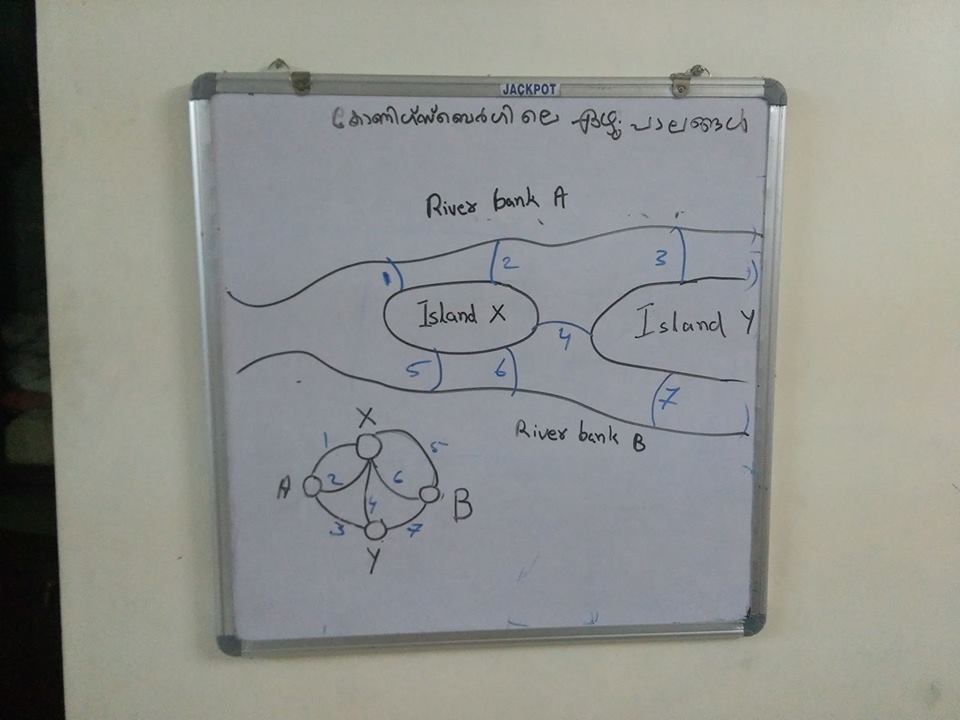
\includegraphics[scale=.25]{images/coni}
\caption{കോണിസ് ബെർഗിലെ പാലങ്ങൾ  }
\label{palam}
\end{figure}

ഇനി പ്രശ്നത്തിലേക്ക് വരാം. നഗരത്തിലെ ഏതെങ്കിലും ഒരു സ്ഥലത്തുനിന്നു പുറപ്പെട്ടു അവിടെത്തന്നെ തിരിച്ചെത്തണം ഓരോ പാലത്തിലും ഒരു തവണ മാത്രമേ കയറാവൂ. ഈ പ്രോ ബ്ലത്തിന് ഒരു സൊലൂഷൻ ഉണ്ടോ ?

1700-കളിൽ പ്രശസ്ത സ്വിസ് ഗണിത ശാസ്ത്രജ്ഞനായ ഒയിലർ റഷ്യയിലെ കാതറിൻ രാജ്ഞിയുടെ അതിഥിയായി മോസ്കോയിൽ ദീർഘകാലം താമസിച്ചിരുന്നു . പാലങ്ങളുടെ പ്രശ്നം ആരോ അദ്ദേഹത്തിന്റെ ശ്രദ്ധയിൽ കൊണ്ടുവന്നു. കോണിസ് ബെർഗിലെ പാലങ്ങളുടെ പ്രശ്നം ഓയിലർ പരിഹരിക്കാൻ നോക്കിയത് ഗണിതത്തിലെ പ്രധാനപ്പെട്ട ഒരു ശാഖയായ ഗ്രാഫ് തിയറിയുടെ പിറവിക്കിടയാക്കി.

ഒരു ഗ്രാഫിൽ പ്രധാനമായും വെർട്ടെക്സുകളും എഡ്ജുകളുമാണുള്ളത്. ഏതെങ്കിലും ഒരു വെർട്ടെക്സിൽ നിന്ന് പുറപ്പെട്ട് എല്ലാ എഡ്ജുകളിലൂടെയും സഞ്ചരിച്ച് പുറപ്പെട്ട വെർട്ടെയിൽത്തന്നെ തിരിച്ചെത്തണം എന്നതാണ് നമ്മുടെ പ്രോബ്ലം. ഇത്തരം വഴികളെ ഒയ്ലീറിയൻ സർക്യൂട്ട് എന്ന് വിളിക്കും.

കോണിസ് ബർഗ് പ്രോ ബ്ലത്തെ ഗ്രാഫിൽ എങ്ങിനെ രേഖപ്പെടുത്താമെന്ന് നോക്കാം. കരകളെ വെർടെക്സ് കളായും പാലങ്ങളെ എഡ്ജുകകയും പരിഗണിച്ചു കൊണ്ടുള്ള ഒരു ഗ്രാഫ് ചിത്രത്തിൽ കാണിച്ചിരിക്കുന്നു.

ഓരോ വെർട്ടെക് സിലും എത്ര ഐഡ്ജുകൾ വന്നു ചേരുന്നു എന്നതിനെ വെർടെക്സിന്റെ ഡിഗ്രി എന്ന് വിളിക്കാം. ചിത്രത്തിലെ A, B Y എന്നി വെർ ടെക്സുകളുടെ ഡിഗ്രി മുന്നാണ് X ന്റെ ഡിഗ്രി അഞ്ചും. ഏതെങ്കിലും ഒരു വെർടെക്സിന്റെ ഡിഗ്രി ഒറ്റ സംഖ്യയായാൽ മേൽ പറഞ്ഞ പ്രകാരമുള്ള നടത്തം (ഒയ്ലി റിയൻ സർക്യൂട്ട് ) സാധ്യമാകില്ല. കാരണം വെർക്കട്ട ക്സിലേക്ക് എത്താനും പുറത്തിറങ്ങാനും ഓരോ എഡ്ജുകൾ വേണം.
ഡിഗ്രി ഒറ്റ സംഖ്യയായാൽ ഒരു എഡ്ജ് മിച്ചം വരും.
ഗ്രാഫ് തിയറിയുംഗ്രാഫ് അൽഗോരിതങ്ങളും കമ്പ്യൂട്ടർ സയൻസിൽ വ്യാപാകമായി ഉപയോഗിക്കുന്നുണ്ട്.
നമ്മുടെ ഫേസ്ബുക്ക് ഗ്രാഫ് തിയറിയുടെ വിലയ ഒരു ഉപഭോക്താവാണ്. നമ്മുടെ പോസ്റ്റും ലൈക്കും ഫ്രണ്ട് ലിസ്റ്റും കമന്റുമെല്ലാം ഫേസ് ബുക്കിന്റെ കണ്ണിൽ വലിയ ഒരു ഗ്രാഫാണ്‌. നെറ്റ്വർക്ക് അനാലിസ് സ്, മെഷിൻ ലേ ർ ണിംഗ് എന്നി ശാസ്ത്ര ശാഖകളിലും ഗ്രാഫ് തിയറി ഉപയോഗിക്കുന്നുണ്ട്.

കോണിസ് ബെർഗിലെ പാലങ്ങളുടെ കഥ ഇതു കൊണ്ട് തീർന്നില്ല ഓയിലർക്ക് ചെയ്യാൻ കഴിയാതിരുന്നത്, റഷ്യൻ പട്ടാളത്തിന് വളരെ എളുപ്പത്തിൽ ചെയ്യാൻ സാധിച്ചു.രണ്ടാം ലോകമഹായുദ്ധത്തിനിടെ അവർ ചില പാലങ്ങൾ ബോംബിട്ട് തകർത്തു. അതോടെ പട്ടണത്തിലെ ഒരു സ്ഥലത്ത് നിന്ന് നടന്ന് എല്ലാ പാലങ്ങളിലും ഒരു തവണ മാത്രം കയറി പുറപ്പെട്ട സ്ഥലത്ത് തിരിച്ചെത്താമെന്നായി. അങ്ങനെയാണെങ്കിൽ ഏതൊക്കെ പാലങ്ങളാകും തകർത്തത് ?

PS: കഥ ഇനിയുമുണ്ട്. സോവിയറ്റ് ഭരണകാലത്ത് പട്ടണത്തിന്റെ പേര് കാലിനിൻ ഗ്രാഡ് എന്നാക്കി മാറ്റി. പഴയര ണ്ടു പലങ്ങൾ ഇടിച്ച് ഹൈവേയാക്കി. ഒന്ന് പുതുക്കിപ്പണിതു. ഇപ്പോൾ പഴയതെന്ന് പറയാൻ രണ്ടേ ബാക്കിയുള്ളു.  
  
  
  \section{ ലെനിൻഗ്രാഡിലെ കഷണ്ടിക്കാർ }
  
  പഴയ സോവിയറ്റ് യുണിയൻ ഗണിത ശാസ്ത്ര പഠനത്തിന് പ്രത്യേക പരിഗണന നൽകിയിരുന്നു. ഗണിത സംബന്ധിയായി നിരവധി പുസ്തകങ്ങളും അവരിറക്കിയിരുന്നു. Mathematical circles ഈ കൂട്ടത്തിലെ പ്രധാന പുസ്തകങ്ങളിലൊന്നാണ്. ഇത് Recreational mathematics ൽ താൽപര്യമുള്ളവർ തീർച്ചയായും വാങ്ങി സൂക്ഷിക്കണം. ഞാനും Vidya യും കൂടി ഇതിലെ ചില കണക്കുകൾ ചെയ്ത് നോക്കുകയാണ്.
  
  \begin{figure}[H]
  \center
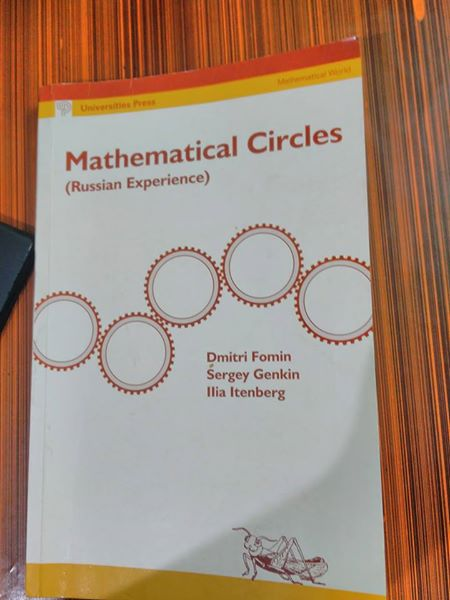
\includegraphics[scale=.25]{images/lenin}
\caption{Mathematical Circles}  
\label{lenin}
\end{figure}
ഇതാ ഒരു സാമ്പിൾ.
ലെനിൻ ഗ്രാഡിൽ ആകെ 50 ലക്ഷം താമസക്കാരുണ്ട്. സർക്കാർ കഷണ്ടി രോഗ ഗവേഷണത്തിന്റെ ഭാഗമായി ആളുകളുടെ തലയിലെ മുടിയിഴകളുടെ എണ്ണം എടുത്തു. പത്തുലക്ഷ ത്തിൽ കൂടുതൽ മുടിയിഴകളുള്ളതാമസക്കാർ ആരുതന്നെ ഇല്ല എന്ന് കണ്ടെത്തി. അങ്ങനെയാണെങ്കിൽ ലെനിൻ ഗ്രാഡി ൽ കുറഞ്ഞത് 2 പേർക്കെങ്കിലിലും തലയിലുള്ള മുടിയുടെ എണ്ണം തുല്യമായിരിക്കും എന്ന് തെളിയിക്കുക.


  \section{എന്താണ് e}

 പ്ലസ്ടു ക്കാരി ഡിഫറൻസിയേഷൻ പഠിക്കുകയാണ്.  ഉറക്കെ ഉരുവിടുന്നു.  derivative of $ e^x = e^x$. കൂടാതെ പത്തു നൂറെണ്ണം ഉണ്ട്. അപ്പോൾ \\
  ഞാൻ : "എന്താണ്  e"\\
 +2 : "അത് ഒയിലർ നമ്പർ" \\ 
 ഞാൻ :  "എന്നു വെച്ചാൽ "\\
 +2  :   "2.71. ...."\\
 ഞാൻ: "ഇതെങ്ങിനെ കിട്ടി." \\
 +2:    :( \\
 ഞാൻ: "എങ്കിൽ ഒരു കൈ നോക്കാം " \\
    ഗണിതത്തിലെ വിവിധ ശാഖകളിൽ സാധാരണ ഉപയോഗിക്കുന്ന ഒരു കോൺസ്റ്റന്റ് ആണ്  ഓയിലർ നമ്പർ എന്ന e. കക്ഷി ഇറാഷണൽ ആണ്. ട്രാൻസെൻഡെന്റലും.  ഏകദേശ വില 2.7182818284590452353602874713527  പൈ പോലെ തന്നെ പല  ഗണിത പ്രശ്നങ്ങളുടേയും സൊലൂഷനിൽ e പ്രത്യക്ഷപ്പെടും. നമുക്ക് e യെ പല  രീതിയിൽ നിർവ്വചിക്കാം. ഇതിൽ ഏറ്റവും എളുപ്പം കൂട്ടു പലിശ കണക്ക്  ഉപയോഗിച്ചാണ്. ഈ രീതി 1683 ജേക്കബ് ബർണൗളിയാണ് കണ്ടെത്തിയത്.

 ഞാൻ നിങ്ങൾക്ക് ഒരു  രൂപ 100 \% പലിശക്ക് കടം തന്നു എന്നിരിക്കട്ടെ. ഒരു വർഷം കഴിയുമ്പോൾ നിങ്ങൾ  എനിക്ക് മുതൽ ഒരു രൂപയും പലിശ ഒരു രൂപയും ചേർത്ത് രണ്ട് രൂപ തരണം.  അടുത്തതായി ഞാൻ നിങ്ങളോട് ആറുമാസത്തിൽ ഒരിക്കൽ പലിശ മുതലിനോട് ചേർക്കണം  എന്നാവശ്യപ്പെടുകയാണ്. ആറു മാസം കഴിയുമ്പോൾ ഒരു രൂപ മുതലും അര രൂപ പലിശയും  ചേർന്ന് 1. 5 രൂപയാകും. അടുത്ത ആറു മാസം ഈ 1. 5 രൂപയുടെ പലിശയാണ്  കൊടുക്കേണ്ടത്. 100 \% നിരക്കിൽ. അപ്പോൾ ഒരു വർഷം കഴിയുമ്പോൽ ആകെത്തുക 1.5+  0.75 = 2.25 ആകും. \\
 എങ്കിൽ പലിശ  മൂന്നു മാസത്തിൽ ഒരിക്കൽ മുതലിനോട് ചേർത്താലോ? നമുക്ക് കൂട്ടി നോക്കാം.\\
 മൂന്നാം മാസം 1+ 1 / 4 = 1.25 \\
 ആറു മാസം  1.25+ 1.25/4 =1.5625 \\
 ഒൻപത് മാസം 1. 5625+ 1.5625/4 =1.953125 \\
 ഒരു വർഷം    1.953125 + 1.953125 / 4 = 2.44140625 \\
 ഒരു വർഷം കഴിഞ്ഞ് നമുക്ക് കിട്ടുന്ന തുക എളുപ്പം കണ്ടു പിടിക്കാൻ  
 $ \textbf{മുതൽ} *  (1+ I / 4) ^ 4 $ എന്ന ഫോർമുല ഉപയോഗിക്കാം. (സംശയമുള്ളവർ കൂട്ടി  നോക്കണം ) ഇവിടെ നാല് എന്നത് എത്ര തവണ  മുതലിനോട് പലിശ കുട്ടി എന്നതാണ്‌.  അങ്ങനെയെങ്കിൽ ഓരോ മാസവും പലിശ മുതൽ കൂടിയാലോ. നമ്മുടെ ഫോർമുല മുതൽ $ * (1+1/12) ^{12}$ എന്നാകും. ആകെത്തുക 2.61303529.  ഇനി ഇതേ കാര്യം ദിവസേന ചെയ്താൽ   മുതൽ $ * (1+ I / 365) ^ {365} $എന്നെടുത്താൽ മതി. കിട്ടാനുള്ള തുക 2.714567482  ആകും.
 
 
 ഒരു വർഷം n തവണ പലിശ കണക്കാക്കിയാൽ  മുതൽ $ * (1+ I / n) ^ n $ രൂപയാകും തിരികെ കിട്ടുക.
ഇനി നമുക്ക് പലിശ മുതലാനോട് കുട്ടിയപ്പോൾ കിട്ടിയ തുകകളെ ഒന്ന് നിരത്തിയെഴുതാം.


  2, 2.25 , 2.44140625, 2.61303529, 2.714567482  എന്നിങ്ങനെയാണ് തുക കൂടിയത്. നിങ്ങൾ n ന്റെ വില  കൂട്ടിയതിനനുസരിച്ച് തിരിച്ചു കിട്ടാനുള്ള തുക കുടുന്നുണ്ടെങ്കിലും , ഈ  വർദ്ധനവിന്റെ നിരക്ക് കുറഞ്ഞ് വരുന്നതായി കാണാം.
നമുക്ക്  n ഒരു പതിനായിരം ഇട്ടു നോക്കാം ഫോർമുല പ്രകാരം ആണ് എനിക്ക് കിട്ടിയത്‌  2.718145927 n ഇൻഫിനിറ്റി യിലേക്ക്  കൂട്ടിയാലും ഒരു നിശ്ചിത തുകക്കപ്പുറം മുതൽ വർദ്ധിക്കില്ല. ഈ ലിമിറ്റാണ്  ഓയിലർ നമ്പർ. മുകളിൽ കൊടുത്തിരിക്കുന്ന 2.7182818284590452353602874713527 e  യുടെ ഏകദേശവിലയാണ്  irrational ആയതു കൊണ്ട് കൃത്യ വില നിശ്ചയിക്കാൻ പറ്റില്ല.  ഗണിത ചിഹ്നങ്ങൾ ഉപയോഗിച്ചാൽ ഇതിനെ താഴെക്കാണുന്ന പ്രകാരം എഴുതാം.

e യുടെ ഒരു ഫോർമുല ചിത്രം  ~\ref{e1}  കാണിച്ചിരിക്കുന്നു.
\begin{figure}
\center
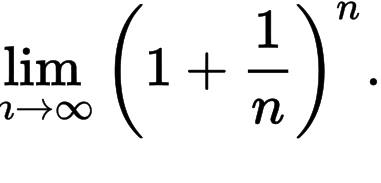
\includegraphics[scale=.25]{images/e}
\caption{e യുടെ  ഫോർമുല }
\label{e1}
\end{figure}
മുകളിൽ  പറഞ്ഞതു e യുടെ ഒരു വിശദീകരണമാണ്. മറ്റൊരു ഫോർമുല ചിത്രം  ~\ref{e2} കാണിച്ചിരിക്കുന്നു.   
  
  \begin{figure}[H]
  \center
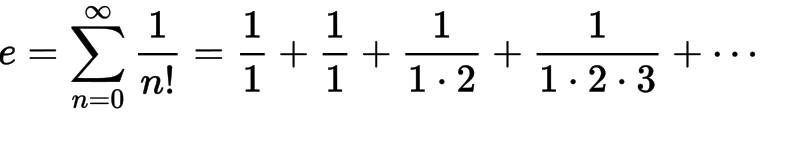
\includegraphics[scale=.25]{images/e1}
\caption{e യുടെ  മറ്റൊരു ഫോർമുല }
\label{e2}
\end{figure}
  
  e യെ നമുക്ക് ഒരു വിസ്തീര്ണമായും പരിഗണിക്കാം. y =1 /x  എന്ന ഫങ്ഷൻ   എടുക്കുക. ചിത്രം ~\ref{e3}   ഷേഡ്  ചെയ്തു കാണിച്ചിരിക്കുന്ന ഭാഗത്തിന്റെ വിസ്തീർണം  ( x = 1 മുതൽ  x = e  വരെ ) ഒന്നായിരിക്കും 
  
    \begin{figure}[H]
  \center
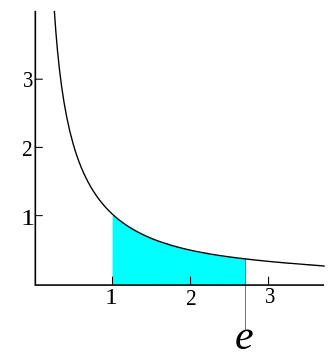
\includegraphics[scale=.25]{images/e2}
\caption{e യുടെ  വില ഒരു വിസ്തീർണമായി  }
\label{e3}
\end{figure}
അതായത് 
\begin{align*}
\int_{1}^{e} \frac{1}{x} dx = 1
\end{align*}


(ഇത് കണ്ടു ഭയപ്പെടരുത്. ചിത്രത്തിലെ അടയാളപ്പെടുത്തിയ ഭാഗത്തെ വിസ്തീർണം   കണ്ടു പിടിക്കേണ്ടതെങ്ങിനെ എന്ന്  ഗണിത ചിഹ്നങ്ങൾ ഉപയോഗിച്ചെഴുതിയതാണ്. ഇന്റഗ്രൽ എന്നണിതിനെ വിളിക്കുന്നത്. പിന്നീട് ഇത് വിശദീകരിക്കാം) 
\section{ഗുണനവും കമ്യൂട്ടേറ്റിവ് നിയമവും}  
  തട്ടിപ്പ്കാട്ടിൽ ഇട്ടുപ്പ് സ്ഥലത്തെ പ്രധാന മുതലാളിയാണ്. തട്ടിപ്പ്കാട്ടിൽ ജുവലേർസ്, തട്ടിപ്പുകാട്ടിൽ ഫൈനാൻസിയേഴ്സ് എന്നിങ്ങനെ പല സ്ഥാപനങ്ങളും നടത്തുന്നുണ്ട് .അപ്പോഴാണ് സർക്കാർ ജി എസ് ടി കൊണ്ടുവന്നത്. മുതലാളി ആകെ പെട്ടു. സർക്കാരിന് ടാക്സ് കൃത്യമായി കൊടുക്കണം. ഇത് പതിവില്ലാത്തതാണ്. പക്ഷേ വേറെ വഴിയില്ല 
\begin{figure}[H]
  \center

\includegraphics[scale=.25]{images/20}
\caption{ഡിസ്കൗണ്ട്}
\label{discount}
\end{figure}
  പക്ഷേ മുതലാളി ആരാ മോൻ. ഇതൊരു അവസരമായി കണ്ടു ജ്വല്ലറിയിലെ എല്ലാ ആഭരണങ്ങൾക്കും 30 ശതമാനം വില കൂട്ടി. എന്നിട്ട് 20 ശതമാനം ഡിസ്കൗണ്ട് പ്രഖ്യാപിച്ചു. നാടുനീളെ ഇങ്ങനെ പരസ്യം എഴുതി വെച്ചു 20\% പ്രത്യേക ഡിസ്കൗണ്ട്. ഡിസ്കൗണ്ടിന് ടാക്സില്ലാത്ത പ്രത്യേക 'വെട്ടിപ്പോ ' സ്വർണ്ണ സമ്പാദ്യ പദ്ധതി. ഇത് കേട്ട ഉടനെ സ്ഥലത്തെ പ്രധാന ബുദ്ധിജീവിയായ നാണു ഭാര്യയേക്കുട്ടി കടയിലെത്തി. ആയിരം രൂപയുടെ മോതിരം വാങ്ങി ബില്ല് അടിക്കാൻ ചെന്നു. കൗണ്ടറിലിരിക്കുന്ന സുന്ദരി ഇങ്ങനെ മൊഴിഞ്ഞു. സർ 10\% മാണ് ജീ എസ് ടി. ഞങ്ങളുടെ കമ്പനിക്ക് പ്രത്യേക ‘വെട്ടിപ്പോ' കാർഡ് പദ്ധതിയുണ്ട്. 100 രൂപാ കൊടുത്ത് മെമ്പറാകാം. പദ്ധതി ഇങ്ങനെയാണ്. നിങ്ങളുടെ ബിൽ തുകയിൽ ഞങ്ങൾ ആദ്യം 20\% ഡിസ്കൗണ്ട് ഇടും. അങ്ങനെ കിട്ടുന്ന തുകയുടെ 10\% ടാക്സ് കൊടുക്കാം. പദ്ധതിയിൽ ചേരാത്തവർക്ക് ബിൽ തുകയിൽ 10\%ടാക്സ് ആദ്യം അടിക്കും അതിന് പുറത്താണ് 20\% ഡിസ്കൗണ്ട്. അപ്പോൾ സർ ‘വെട്ടിപ്പോ ‘ കാർഡ് എടുക്കുകയല്ലെ ? ചോദ്യം ഇതാണ്. കാർഡ് കൊണ്ട് ആർക്കാണ് ലാഭം? 
  
  ഉത്തരം കിട്ടിക്കാണുമെന്ന് കരുതുന്നു. ഗുണനം (multiplication) കമ്യൂട്ടേറ്റീവ് (commutative) ആണ്. രണ്ട് സംഖ്യകളെത്തമ്മിൽ ഗുണിക്കുമ്പോൾ സംഖകളുടെ ഓഡർ ഉത്തരത്തിൽ വ്യത്യാസം ഉണ്ടാക്കുന്നില്ല. ഉദാഹരണത്തിന് $8 * 4 = 4 * 8$ കുറേക്കൂടി അബ്സ്ട്രാക്ടായി $a * b = b * a$ എന്നെഴുതും. a യും b യും ഏത് റിയൽ നമ്പറായാലും ഈ സമവാക്യം ശരിയാണ്. ഇനി മുതലാളി ടാക്സും ഡിസ്കൗണ്ടും കൊടുക്കുമ്പോൾ എന്താണ് സംഭവിക്കുന്നതെന്ന് നോക്കാം. 
  
  നമുക്ക് മാലയുടെ വില a എന്ന് എടുക്കാം. ആദ്യം 10\% ടാക്സ് കൊടുക്കുമ്പോൾ a + 0.1 a ആണ് നാം കൊടുക്കേണ്ട ആകെ തുക. 
  
 $ a+ 0. 1 a = (1 +0.1) a = 1.1 a$  
  
  ഈ തുകയുടെ പുറത്താണ് 20 \% ഡിസ്കൗണ്ട്. അതായത് ബിൽ തുകയുടെ 80 \% മാത്രമേ കൊടുക്കേണ്ടതുള്ളു. 
  
  $1.1 * a * 0.8 $ ആണ് ഡിസ്കൗണ്ടിന് ശേഷം നമ്മൾ മുതലാളിക്ക് കൊടുക്കുന്നത്. ഇനി ആദ്യം ഡിസ്കൗണ്ട് ഇടുകയാണെങ്കിൽ വില $0.8 * a$ ആകും. ഇതിന്റെ 10\% ടാക്സ് കൂടി ചേർത്താൽ ആകെത്തുക $0.8 *a + 0.8 * a * 0.1$ ആണ്. 
  
 $ 0.8 * a + 0.8 * a * 0.1 = (1 +0.1) 0.8 a = 1.1 * 0.8 * a$ ഇത് ആദ്യം കാട്ടിയ സംഖ്യ തന്നെയാണ്. ചുരുക്കത്തിൽ $a * b * c = b  * c * a = c * b * a  = ... $ബാക്കി നിങ്ങൾക്ക് പൂരിപ്പിക്കാം. 
\section{
 എന്താണി ഡിറ്റർമിനന്റ്?  }  
  പ്ലസ് 2ക്കാരിയുടെ ചോദ്യമാണ്. കക്ഷി രണ്ടു ദിവസമായി മെട്രിക്സുകളോട് മല്ലു യുദ്ധത്തിലാണ്. മെട്രിക്സുകളെ കൂട്ടുന്നു കുറക്കുന്നു തിരിച്ചും മറിച്ചുമിട്ട് ഗുണിക്കുന്നു. അതൊന്നും വലിയ കുഴപ്പമില്ല.പക്ഷെ മെട്രിക്സിന്റെ ഡിറ്റർമിനന്റ് എത്തിയപ്പോൾ കുടുങ്ങി. അങ്ങോട്ടുമിങ്ങോട്ടും സംഖ്യകൾ തമ്മിൽ ഗുണിക്കും കൂട്ടും കറക്കും കാര്യമെന്താണെന്ന് മാത്രം അറിയില്ല. ടീച്ചർ 4 X 4 മെട്രിക്സ് ഒക്കെ ഹോം വർക്ക് കൊടുത്തിട്ടുണ്ട്. പക്ഷെ എന്തിനാണി ഡിറ്റർമിനന്റ് കണ്ടു പിടിക്കുന്നത് എന്നു മാത്രം പറഞ്ഞില്ല. എൻജിനിയറിംഗ് യജ്ഞം മുക്കാൽ പങ്കും പൂർത്തിയാക്കിയ ശേഷക്കാരന്റെയടുത്ത് സംശയമെത്തി. അവിടെയും രക്ഷയില്ല. അങ്ങനെയാണ് ഇന്നലെ കുടുംബസദസിൽ ഡിറ്റർമിനന്റ് കടന്നുവന്നത്. 
  
  ഞാൻ ചെറിയ ഒരു മൈതാന പ്രസംഗം കാച്ചി. അതേകദേശം ഇങ്ങനെയാണ്. ഗണിതം ഭൂഗോളത്തിന്റെ സ്പന്ദനമാണെന്ന് സ്പടികം സിനിമയിൽ ചാക്കോ മാഷ് പറയുന്നുണ്ട്. പക്ഷെ നമ്മൾ സ്കൂളിലും കോളേജിലും ഗണിതം പഠിപ്പിക്കുന്ന രീതിക്ക് എന്തോ കുഴപ്പമുണ്ട്. കുട്ടികൾ യാത്രകമായി കാര്യങ്ങൾ ചെയ്യും. ഒരു ഗണിത രീതി കൊണ്ട് എന്താണ് ഉദ്ദേശിക്കുന്നതെന്ന് പഠിക്കാറില്ല. പഠിപ്പിക്കാറും. ഗണിതം ലോകത്തിന്റെ സ്പന്ദനം തന്നെയാണ്, കാര്യം മനസ്സിലാക്കിയാൽ.ഇല്ലെങ്കിൽ കുട്ടികൾ കണക്ക് വെറുക്കും അഭിനവ ചാക്കോ മാഷ് മാർ കോപിക്കരുത്. ഇത് ഒരു സത്യമാണ്. 
  
  പ്രസംഗം കഴിഞ്ഞ സ്ഥിതിക്ക് കാര്യത്തിലേക്ക് കടക്കാം. ശരിക്കും എന്താണി ഡിറ്റർമിനന്റ്? ആദ്യം നമുക്ക് ചെറിയ ഒരു മെട്രിക്സ് എടുത്ത് അതിൽ നിന്ന് ഡിറ്റർമിനന്റ് കണ്ടു പിടിക്കാൻ ചാക്കോ സാർ പറഞ്ഞു തന്ന വഴി എന്താണെന്ന് നോക്കാം. ചിത്രം \ref{mat1} ഒരു 2x 2 മെട്രിക്സ് കാണിച്ചിരിക്കുന്നു. ഇതിന്റെ ഡിറ്റർമിനന്റ്det A= (ad -bc) യാണ്. വലിയ മെട്രിക് സുകൾക്ക് കുറേക്കൂടി വലിയ ഒരു ഫോർമുല ഉണ്ട്. ഇത് കാണാതെ പഠിച്ച് പരീക്ഷയെഴുതുകയാണ് പിള്ളേർ ചെയ്യുന്നത്.
  
                    
    \begin{figure}[H]
  \center
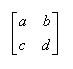
\includegraphics[scale=.5]{images/m1}
\label{mat1}
\caption{2 X 2 മെട്രിക്സ്}
\end{figure}
   ഡിറ്റർമിനന്റിന്റെ പുറകിലുള്ള ആശയം മനസ്സിലാക്കുന്നതിന് ചിത്രം \ref{mat2} പരിഗണിക്കുക. നമ്മുടെ മെട്രിക്സിലെ രണ്ടു നിരകളെ കാർട്ടിഷ്യൻ പ്രതലത്തിലുള്ള രണ്ട് ബിന്ദുക്കളായി ഈ ചിത്രത്തിൽ രേഖപ്പെടുത്തിയിരിക്കുന്നു. O എന്ന് കാണിച്ചിരിക്കുന്നതാണ് പ്രതലത്തിന്റെ ഒറിജിൻ (0, 0).(a b), (c d) എന്നീ ബിന്ദുക്കളിലേക്ക് ഒറിജിനിൽ നിന്ന് രണ്ട് വരകൾ ചിത്രം \ref{mat3}  കാണിച്ചിരിക്കുന്നതു പോലെ വരക്കാം ഇങ്ങനെ വരച്ച വരകളെ നമ്മുക്ക് ഒരു വെക്ടർ എന്ന് വിളിക്കാം. നമ്മുടെ പ്രതലത്തിലേ ഓരോ ബിന്ദുവിലേക്കും ഒരു വെക്ടർ വരക്കാൻ സാധിക്കും. ഓരോവെക്ടറിനും നീളവും ദിശയുമുണ്ട്. ഇനി ചിത്രം നാലിലേതുപോലെ നമ്മൾ വരച്ച വെക്ടറുകളുടെ അഗ്രത്തിൽ നിന്ന് ഒരു പാരലോഗ്രാം വരക്കുക. നമ്മൾ അന്യോഷിച്ചു കൊണ്ടിരിക്കുന്ന ഡിറ്റർമിനന്റ് ഈ പാരലോഗ്രത്തിന്റെ വിസ്തീർണമാണ്.
   
                       
    \begin{figure}[H]
  \center
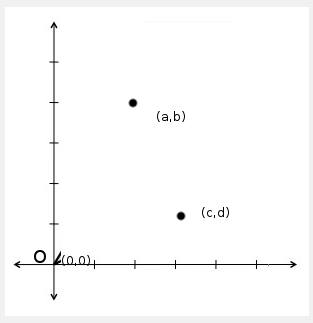
\includegraphics[scale=.5]{images/m2}
\label{mat2}
\caption{ ഡിറ്റർമിനന്റിന്റെ  ആശയം points }
\end{figure}
   
                        
    \begin{figure}[H]
  \center
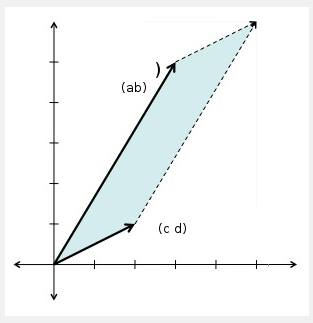
\includegraphics[scale=.5]{images/m3}
\label{mat3}
\caption{ ഡിറ്റർമിനന്റിന്റെ  ആശയം vectors }
\end{figure}
   
    ചുരുക്കത്തിൽ പറഞ്ഞാൽ നമ്മുടെ 2 X 2 മെട്രിക്സിന്റെ നിര വെക്ടറുകൾ അടുത്തടുത്ത വശങ്ങളായി വരുന്ന ഒരു പാര ലോഗ്രത്തിന്റെ വിസ്തീർണമാണ് ഡിറ്റർമിന്റ്. ഈ ആശയത്തെ നമുക്ക് വലിയ മെട്രിക് സുകളുടെ കാര്യത്തിലും വിപുലപ്പെടുത്തി ഉപയോഗിക്കാം. അതിനു മുൻപ് നമുക്ക് മേൽ പ്രസ്താവന ശരിയാണെന്നതിന് തെളിവ് വേണം. തെളിവില്ലാത്ത കാര്യങ്ങൾ വെറും ഊഹാപോഹങ്ങളല്ലെ. തെളിവ് ഉണ്ടാക്കുന്നതിന് ചിത്രം അഞ്ചിൽ കാണിച്ചിരിക്കുന്നതു പോലെ പാരലോഗ്രത്തിന് ചുറ്റും ഒരു ദീർ ഘചതുരം വരക്കുക.ഈ ച തുരത്തിന്റെ ഒരു മൂല ഒറിജിനും മറ്റേ മൂല ( a + c, b+d) എന്ന ബിന്ദുവുമാണ്. മറ്റ് മൂലകളുടെ കോർഡിനേറ്റുകളും ചിത്രത്തിൽ ഉണ്ട്. ഇത് കണ്ടു പിടിച്ച വിധം പിടികിട്ടാത്തവർ ജോമട്രി ക്ലാസിൽ ഒന്നു കൂടിയിരിക്കണം. തുടർന്ന് വായിക്കണമെന്നുമില്ല. എൻജിനിയറിംഗ് വിദ്യർത്ഥിയാണെങ്കിൽ വേറെ ഏതെങ്കിലും കോഴ്സ് ചെയ്യുന്നതിനേക്കുറിച്ച് ഗൗരവമായി ആലോചിക്കണം.
                           
    \begin{figure}[H]
  \center
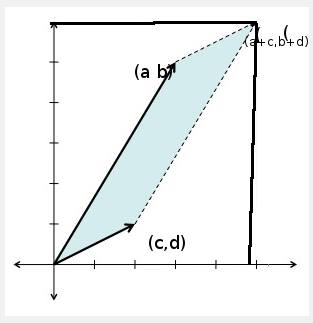
\includegraphics[scale=.5]{images/m4}
\label{mat4}
\caption{ ഡിറ്റർമിനന്റിന്റെ  ആശയം vectors }
\end{figure}
                           
    \begin{figure}[H]
  \center
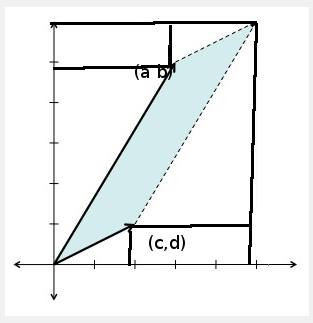
\includegraphics[scale=.5]{images/m5}
\label{mat5}
\caption{ ഡിറ്റർമിനന്റിന്റെ  ആശയം vectors }
\end{figure}
     ഡിറ്റർമിനന്റ് പരലോഗ്രത്തിന്റെ വിസ്തീർണമാണെന്നാണല്ലൊ നേരത്തെ പറഞ്ഞത്. ഈ വിസ്തീർണ്ണം കണ്ടു പിടിക്കാൻ ചിത്രം അഞ്ചിലെ ദീർഘചതുരത്തിന്റെ വിസ്തീർണത്തിൽ നിന്ന് പാരലോഗ്രാം ഒഴികെയുള്ള ഭാഗത്തിന്റെ വിസ്തീർണ്ണം കുറച്ചാൽ മതി ചിത്രം ആറിൽ ഇങ്ങനെ കുറക്കേണ്ട ഭാഗം അടയാളപ്പെടുത്തിയിരിക്കുന്നു. അടയാളപ്പെടുത്തിയ ഭാഗങ്ങളെ നമുക്ക് ചതുരങ്ങളായും ത്രികോണങ്ങളായും തിരിക്കാം. ചിത്രം ആറ് നോക്കിയാൽ ഇത് രേഖപ്പെടുത്തിയിരിക്കുന്നത് കാണാം. പാരലോഗ്രത്തിന്റെ മുകളിലുള്ള ഭാഗവും താഴെയുള്ള ഭാഗവും ഒരേ വിസ്തീർണമുള്ളവയാണെന്ന് കാണാം. ഓരോ ഭാഗത്തും ഒരു ചതുരവും രണ്ട് ത്രികോണങ്ങളുമുണ്ട്.ഇവയുടെ വിസ്തീർണ്ണം വളരെ എളുപ്പത്തിൽ കണ്ടെത്താം. ഇവയുടെ നീളവും വീതിയും ചിത്രത്തിലുണ്ട്. പാരലോഗ്രത്തിന്റെ വിസ്തീർണ്ണം = ദീർഘചതുരത്തിന്റെ വിസ്തീർണ്ണം - ബാക്കി ഭാഗത്തിന്റെ വിസ്തീർണ്ണം ഇത് താഴെക്കാണുന്ന വിധത്തിൽ എഴുതാം ഇപ്പോൾ തെളിഞ്ഞില്ലെ? 
     
                            
    \begin{figure}[H]
  \center
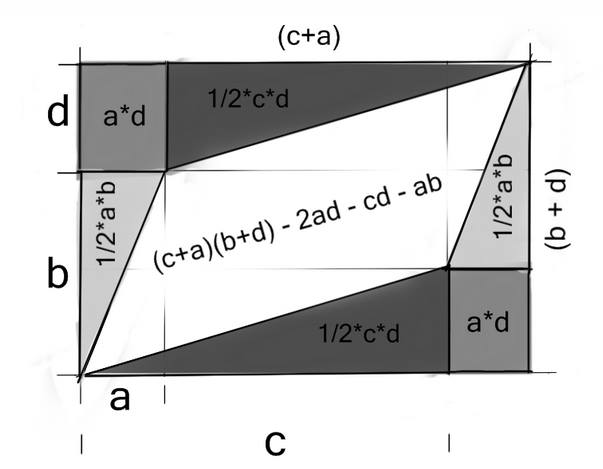
\includegraphics[scale=.4]{images/m6}
\label{mat6}
\caption{ ഡിറ്റർമിനന്റിന്റെ  ആശയം vectors }
\end{figure}
     ഇനി ഒരു 3 x 3 മെട്രിക്സിന്റെ കാര്യം നോക്കാം.ഇതിനായി 3 ഡൈമെൻഷനുള്ള ഒരു കോർഡിനേറ്റ് സിസ്റ്റം പരിഗണിക്കുക. മെട്രിക് സിന്റെ ഓരോ നിരയും ഈ സ്പേസിലെ ഓരോ ബിന്ദുക്കളാണ്. മുൻപത്തേ പോലെ ഒറിജിനിൽ നിന്ന് ഈ പോയിന്റ് കളിലേക്ക് വെക്ടറുകളെ വരക്കാനാകും. തുടർന്ന് ഈ വെക്ടറുകൾ അടുത്തടുത്ത് വരത്തക്ക രീതിയിൽ ഒരു ത്രിമാന രൂപം നിർമിക്കാനാകും. ചിത്രം \ref{mat7} ൽ ഇത് കാണിച്ചിട്ടുണ്ട്. ഈ രുപത്തെ പാരലോെപൈപിഡ് എന്നാണ് വിളിക്കുന്നത്. ഈ പാരലോപൈപ്പി ഡിന്റെ വ്യാപ്തമാണ് 3 X 3 മെട്രിക്സിന്റ ഡിറ്റർമിനന്റ്. ഇതിലും വലിപ്പമുള്ള മെട്രിക് സുകളുണ്ടല്ലോ. അവയുടെ ഡിറ്റർമാന്റ് എന്താണ്. നമുക്ക് മൂന്ന് ഡൈമെൻഷനുകളേ കാണാൻ കഴിയും. 
                                 
    \begin{figure}[H]
  \center
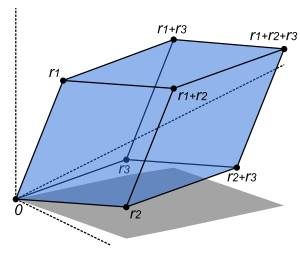
\includegraphics[scale=.5]{images/m7}
\label{mat7}
\caption{ ഡിറ്റർമിനന്റിന്റെ  ആശയം 3 D }
\end{figure}
     പക്ഷെ കൂടുതൽ ഡൈമെൻഷൻ ഉള്ള സ്പേസുകളെ ഗണിത ശാസ്ത്രജ്ഞർ നിർവചിച്ചിട്ടുണ്ട്. മെട്രിക്സ് തിയറി /ലിനിയർ ഒൾജിബ്രാ n ഡൈമെൻഷനൽ സ്പേസുകളെക്കുറിച്ചുള്ള പഠനമാണ്. അതു കൊണ്ട് മേൽ പറഞ്ഞ ആശയം കൂടുതൽ വലിപ്പമുള്ള മെട്രിക്സുകളിലേക്ക് വിപുലികരിക്കാം. പക്ഷെ നമുക്ക് പടം ഉപയോഗിച്ച് വിശദീകരിക്കാനാവില്ല എന്നു മാത്രം. സംഗതി അബ്സ്ട്രാക്ട് ആണ്. എൻജിനിയറിംഗിലും മറ്റ് ശാസ്ത്ര വിഷയങ്ങളിലും ധാരാളം ഉപയോഗമുള്ള ഗണിതശാഖയാണിത്. കൂടുതൽ അറിയാൻ താൽപര്യമുള്ളവർക്ക് MIT പ്രൊഫസറായ ഗിൽബർട്ട് സ്ട്രാങ്ങിന്റെ വിഡിയോ കാണാം.
     
      ആശയങ്ങൾവ്യക്തമായി മനസിലാക്കി പഠിച്ചാൽ ഗണിതം ഭൂലോകത്തിന്റെ സ്പന്ദനവുമാണെന്ന് ചാക്കോ മാഷിന് മാത്രമല്ല നമുക്കും ബോധ്യമാകും.
  
\section{പരന്ന ഭൂമി }

വായനയുടെ സൂക്കേട് പിടിച്ചത് ആറാം ക്ലാസിൽ പഠിക്കുമ്പോഴാണ്. അന്നുതൊട്ട് വായിച്ച് തള്ളിയതിന് കണക്കില്ല ആദ്യമൊക്കെ ഫിക്ഷൻ കുറെക്കഴിഞ്ഞപ്പോൾ ശാസ്ത്രം, ചരിത്രം എന്നിവയിലായിരുന്നു താൽപര്യം. ഞാൻ ജനിച്ചു വളർന്ന ഇടുക്കിയിൽ പുസ്തകങ്ങൾ കിട്ടാൻ നിന്നെ ബുദ്ധിമുട്ടണമായിരുന്നു. ഇതിന് മാറ്റം വന്നത് കോതമംഗലം എൻജിനിയറിംഗ് കോളേജിൽ ചേർന്നപ്പോഴാണ്. അവിടുത്തെ ഹോസ്റ്റൽ കേരളത്തിന്റെ ഒരു പരിഛേദമായിരുന്നു. പുസ്തകവായനക്കാർ പലരുണ്ടായിരുന്നു. കൂടാതെ ഈ സമയത്ത് എനിക്ക് യൂണിവേർസിറ്റി മെരിറ്റ് സ്കോളർഷിപ്പും കിട്ടി. വർഷം ആയിരം രൂപ. മൂന്നു മാസത്തെ ഹോസ്റ്റൽ ഫീസ് കൊടുക്കാം. എത്രയാണ് കിട്ടുന്നതെന്ന് വീട്ടുകാർക്ക് വലിയ പിടിയില്ലാത്തതിനാൽ തുക മിക്കവാറും സിനിമ കണ്ടും പുസ്തകം വാങ്ങിയും തീർക്കും. കലാകൗമുദിയൊക്കെ സ്വന്തമായി വാങ്ങിത്തുടങ്ങിയത് ഇക്കാലത്താണ്. ഇടക്കൊക്കെ എർണാകുളത്ത് കറങ്ങും ബ്രോഡ്വേയുടെ തുടക്കത്തിലുള്ള പൈകോയാണ് പ്രധാന ലക്ഷ്യം. ഇക്കാലത്ത് വായിച്ച പലതും പിന്നീട് സമൂഹത്തേയും സംഭവങ്ങളേയും നിരീക്ഷിക്കുന്നതിലും അഭിപ്രായങ്ങൾ രൂപീകരിക്കുന്നതിലും വലിയ സ്വാധീനം ചെലുത്തിയിട്ടുണ്ട്. ഞാൻ വായിച്ചു ശേഷം മറന്നു പോയ ചില പുസ്തകങ്ങളെ ഒർത്തെടുക്കാൻ ഒരു ശ്രമം തുടങ്ങുകയാണ്. സംഗതി ഓർമ്മയിൽ നിന്നാണ്. തെറ്റുണ്ടെങ്കിൽ സദയം പൊറുക്കുക.
    \begin{figure}[H]
  \center
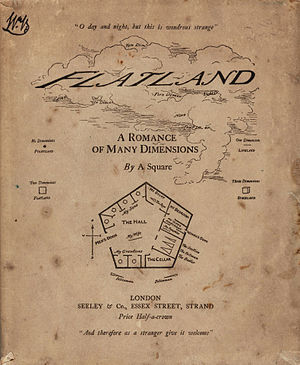
\includegraphics[scale=.7]{images/flatland}
\label{flat1}
\caption{  ഫ്ലാറ്റ്  ലാൻഡ് }
\end{figure}
 ഫ്ലാറ്റ്ലാന്റ് എഡ്വിൻ ആബോട് എഴുതി 1884 ൽ പുറത്തിറങ്ങിയ സറ്റയർ ജോൺറെയിലുള്ള ഒരു നോവലാണ്. കഥാപാത്രങ്ങൾ എല്ലാം ജോമട്രിക്കൽ രൂപങ്ങളാണ്. എല്ലാവരും ദ്വിമാന ലോകത്താണ് ജീവിക്കുന്നത് . സ്ത്രീകൾ എല്ലാം നേർരേഖകളാണ്. പുരുഷൻമാർ പോളിഗണുകളും. കഥ പറയുന്നത് ഒരു ചതുരമാണ്. ഈ ദ്വിമാന ലോകത്ത് നമ്മുടെ ഇന്ത്യയിലെ പോലെ പല തരം ജാതി ഹൈരാർക്കികളുണ്ട്. താഴ്ന്ന ജാതിയിൽ പെട്ട ഇന്റലകടുകളെ പറ്റുമെങ്കിൽ കൊന്നുകളയും അല്ലെങ്കിൽ ഉയർന്ന ജാതിയിൽ ചേർക്കും. കഥ പറയുന്ന ചതുരം ജയിലിലാണ്. കുറ്റം മുന്നാമത് ഒരു ഡൈമെൻഷൻ ഉണ്ട് എന്ന് ദ്വിമാന ലോകത്ത് പ്രചരിപ്പിക്കാൻ ശ്രമിച്ചതാണ്. കഥ തുടങ്ങുന്നത് ദ്വിമാന ലോകത്തിന്റെ വിവരണത്തോടെയാണ്. തുടർന്ന് അവിടുത്തെചരിത്രം വീടുകൾ കാലാവസ്ഥ എന്നിവ വിവരിക്കുന്നു. ചതുരത്തിന് ഗോളത്തേക്കുറിച്ച് വെളിപാടുണ്ടാകുന്നു. ഗോളം ചതുരത്തെ മൂന്നാം മാനത്തെക്കുറിച്ച് ബോധവൽക്കരിക്കുന്നു. ചതുരംതന്റെ പുതിയ സിദ്ധാന്തം പ്രചരിപ്പിക്കാൻ ശ്രമിക്കുന്നതോടെ ഭരണകൂടം ഇടപെടുന്നു.തുടർന്ന് സമകാലിന ഇന്ത്യയിലെ പോലെ കുറെ സംഭവങ്ങൾ. അവസാനം പല ജ്യാമിതീയ രൂപങ്ങളളേയു (ജാതിയനുസരിച്ച് ) കുട്ടക്കൊലക്കും ജയിൽ വാസത്തിനും ശിക്ഷിക്കന്നു. ജയിലിലാകുന്ന ചതുരത്തിന്റെ ഒർമ്മക്കുറിപ്പായിട്ടാണ് കഥ എഴുതിയിരിക്കുന്നത്. വിക്ടോറിയൻ കാലത്തെ വംശ വ്യവസ്ഥയെയും സ്ത്രീകളുടെ പദവിയേയും ഗ്രന്ഥകാരൻ ചിത്രീകരിക്കുന്നു. വർത്തമാനകാലത്തെ പല സംഭവങ്ങളും വിവേചനങ്ങളും കാണുമ്പോൾ എനിക്ക് പണ്ടെന്നോ വായിച്ച ഫ്ലാറ്റ്ലാന്റ് ഓർമ്മ വരും. നിറയെ പടങ്ങളുള്ള ഒരുപഴയ കോപ്പി കയ്യിലുണ്ടായിരുന്നു. ഇന്നലെ നോക്കിയിട്ട് കണ്ടില്ല. Pട. പ്രോജക്ട് ഗുട്ടൻബർഗിൽ ഫ്ലാറ്റ്ലാന്റിന്റെ കോപ്പിയുണ്ട്. ഒരു അനിമേഷൻ സിനിമയും ഇറങ്ങിയിട്ടുണ്ട്. യൂ ട്യൂബിൽ നോക്കിയിട്ട് കണ്ടെത്താനായില്ല.
  \begin{figure}[H]
  \center
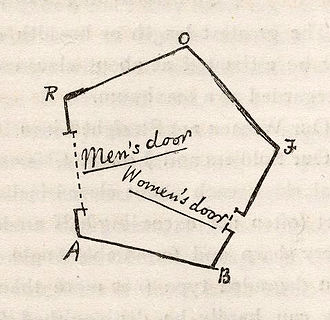
\includegraphics[scale=.7]{images/flat1}
\label{flat2}
\caption{  ഫ്ലാറ്റ്  ലാൻഡിലെ വീട്  }
\end{figure}

\section{നെപ്പോളിയൻ തിയറം To be rewritten}

  ക്ലാസിക്കൽ ജോമെട്രിയിലെ മിക്കവാറും തിയറങ്ങളും പുരാതന ഗ്രീക്ക് ഗണിത ശാസ്ത്രജ്ഞന്മാരുടെ സംഭാവനയാണ്. യുക്ലിഡ് പൈതഗോറസ് ഒക്കെ ചെറിയ ക്ലാസുകളിൽ നമുക്ക് പേടി സ്വപ്നമായിരുന്നത് ഇതിനാലാണ്. എന്നാൽ സാക്ഷാൽ തെപ്പോളിയന്റെ പേരിൽ ഒരു തിയറമുണ്ട്. നെപ്പോളിയാണ് കണ്ടു പിടിച്ചതെന്നുള്ളതിന് വ്യക്തമായ തെളിവില്ല. എങ്കിലും നെപ്പോളിയന്റെ ജീവിതകാലത്താണ് ഈ തിയറം പ്രത്യക്ഷപ്പെട്ടിട്ടുള്ളത്. തിയറം ഇങ്ങനെയാണ്. ABC ഒരു ത്രികോണമാണ്‌. ABC യുടെ വശങ്ങൾ ഉപയോഗിച്ച് ചിത്രത്തിലുള്ളതുപോലെ മൂന്ന്equi lateral triangles വരക്കുക. ചിത്രത്തിൽ Acy BC x ABZ എന്നീ ത്രികോണങ്ങളാണവ. ഈ മുന്ന്ത്രികോണങ്ങളുടെയും centre MNL എന്ന് അടയാള പ്പെടുത്തിയിരിക്കുന്നു. നെപ്പോളിയൻ തിയറപ്രകാരം MNL എപ്പോഴും ഒരു equilateral ത്രികോണമായിരിക്കും. . ത്രികോണമിതി യു പയോഗിച്ചും കോംപ്ലക്സ് നമ്പർ ഉപയോഗിച്ചും ഈ തിയറം തെളിയിക്കാം. 

  \begin{figure}[H]
  \center
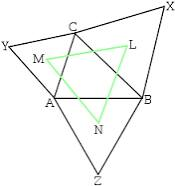
\includegraphics[scale=.7]{images/nap}
\label{nap}
\caption{  നെപ്പോളിയൻ തിയറം }
\end{figure}
\section{ബാറിലേക്കുള്ള ദൂരവും ടാക്സി കാബ് ജോമെട്രിയും.}
സുപ്രീം കോടതി വിധിയേത്തുടർന്ന് പാതയോരത്തെ ബാറുകൾക്ക് പുട്ടുവീഴുമെന്നായപ്പോൾ പലരും വാതിൽ മാറ്റി വെച്ചും വഴി മാറ്റിയും പ്രവർത്തനം തുടരാൻ ശ്രമിക്കുന്ന കാര്യം മാധ്യമങ്ങളിൽ വാർത്തയാണല്ലൊ. ഈ വാർത്തയോടൊപ്പം പറവൂരുള്ള ഒരു ബാറിലേക്ക് പണിത വഴിയും കൊടുത്തിട്ടുണ്ട്. (ചിത്രം ~\ref{bar1}). 500 മീറ്റർ ദൂരം കിട്ടാൻ വളഞ്ഞുപുളഞ്ഞ വഴി കെട്ടിയെടുത്ത വിദ്വാൻ ഇക്കാര്യം ആരെങ്കിലും കോടതിക്കു മുന്നിൽ ഉന്നയിക്കുമ്പോൾ ഉയർത്തുന്ന എതിർ  വാദം എന്തായിരിക്കുമെന്ന് ആലോചിച്ചിട്ടുണ്ടോ. 
 

 \begin{figure}[H]
  \center
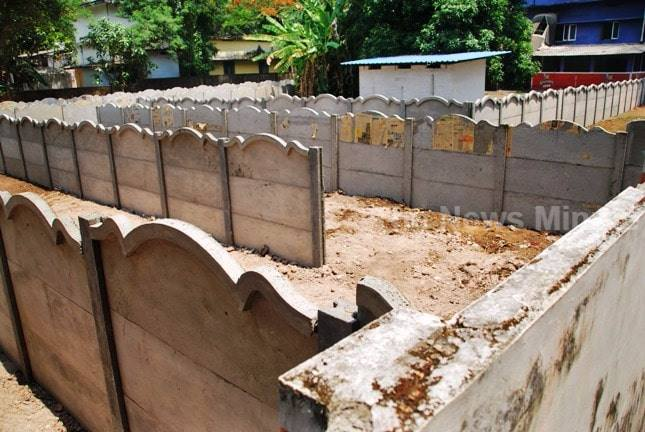
\includegraphics[scale=.25]{images/bar1}
\label{bar1}
\caption{   ബാറിലേക്കുള്ള വഴി }
\end{figure}

ദൂരം (distance) നാമൊക്കെ സാധാരണയായി നിർവ്വചിക്കുന്നത് യൂക്ലിഡിയൻ രീതിയിലാണ്. അതായത് പോയിന്റ് A യിൽ നിന്ന് പോയിന്റ് B യിലേക്ക് വരക്കുന്ന നേർരേഖയുടെ നീളമാണ് നാം ദൂരമായി കരുതുന്നത്.  ഈ യൂക്ലിഡിയൻ ദൂരമാണ് നമ്മൾ സ്കൂളിൽ പഠിച്ച ജോമട്രിയുടെ അടിസ്ഥാനം. വിധി പറഞ്ഞ ജഡ്ജി ഈ രീതിയിൽ മാത്രമേ ദൂരം അളക്കാൻ കഴിയു എന്ന് ധരിച്ചിട്ടുണ്ടാകണം. 

             ഇനി തിരുവനന്തപുരത്തുനിന്ന് എർണാകുളത്തേക്കുള്ള ദൂരം പരിഗണിക്കുക. NH 66 വഴി 204.3 കിലോമീറ്റർ ദൂരമാണ് ഗൂഗിളിൽ കാണുന്നത്. ഇത് യൂക്ലിഡിയൻ ഡിസ്റ്റൻസ് ആണോ. അല്ല. എർണാകുളത്തെത്താൻ റോഡിലൂടെ വണ്ടി ഓടിക്കേണ്ട ദൂരമാണ് ഈ 204.3 കി.മി. ഇങ്ങനെ നോക്കിയാൽ ബാറുടമയുടെ വാദം നമ്മൾ ശരിവെക്കേണ്ടി വരും.
         \begin{figure}[H]
  \center
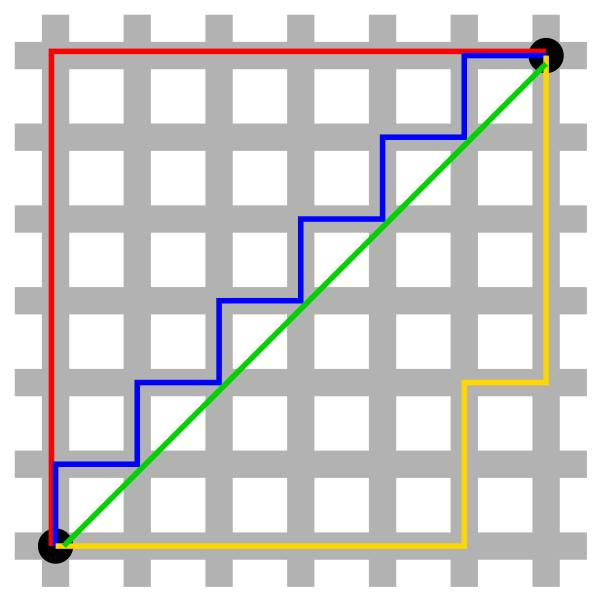
\includegraphics[scale=.25]{images/bar2}
\label{bar2}
\caption{   ബാറിലേക്കുള്ള വഴി }
\end{figure}     
            ഗണിത ശാസ്ത്രത്തിൽ യൂക്ലിഡിയൻ ദൂരത്തിന് പുറമെ മറ്റ് പലതരം ദൂരങ്ങളേയും നിർവചിച്ചിട്ടുണ്ട്.   ഉദാഹരണത്തിന്  കമ്പ്യൂട്ടർ വിഷൻ  മെഷീൻ ലേർണിംഗ് തുടങ്ങിയ മേഖലകളിൽ വ്യാപകമായി ഉപയോഗിക്കുന്ന  ടാക്സി കാബ് ദൂരം  ഉപയോഗിച്ചാണ് അളന്നതെന്ന്  ബാറുടമക്ക് വാദിക്കാം. ഇതെന്താണെന്നറിയണമെങ്കിൽ ചിത്രം രണ്ട് പരിഗണിക്കുക. ഇതിൽ നമ്മുക്ക് സഞ്ചരിക്കാവുന്ന വഴികളെ ഒരു ഗ്രിഡ് ആയി കാണിച്ചിരിക്കുന്നു.  ( പ്ലാൻ ചെയ്ത് പണിത ഒരു പട്ടണത്തിലെ റോഡുകളാണ് ഈ ഗ്രിഡ് എന്ന് കരുതുക ).  ഇതിൽ കറുത്ത നിറത്തിൽ കാണിച്ചിരിക്കുന്ന രണ്ട് പോയിന്റുകൾക്കിടയിൽ പല വഴികളുണ്ട്. ഒരു ടാക്സി കാർ ഇവക്ക് ഇടയിൽ സഞ്ചരിക്കുകയാണെന്ന് സങ്കൽപിക്കുക. കാർ സഞ്ചരിക്കേണ്ട കുറഞ്ഞ ദൂരമാണ് ടാക്സി കാബ് ഡിസ്റ്റൻസ്. ചിത്രത്തിൽ ചുവപ്പ് മഞ്ഞ നീല എന്നിങ്ങനെ മൂന്ന് നിറങ്ങളിൽ ഇത് അടയാളപ്പെടുത്തിയിട്ടുണ്ട്.  ഈ മൂന്ന് വഴികൾക്കും ഒരേ ദൂരമാണ്.  പച്ചനിറത്തിലുള്ളതാണ് യൂക്ലിഡിയൻ  ദൂരം.
 

      പത്തൊൻപതാം നൂറ്റാണ്ടിൽ ജീവിച്ചിരുന്ന ജർമൻ ഗണിത ശാസ്ത്രജ്ഞനായ ഹെർമൻ മിൻകോവിസ്കിയാണ് ഇത്തരത്തിലുള്ള ജോമട്രിയെക്കുറിച്ച് വിശദമായി പഠിച്ചത്.   ഇങ്ങനെ  ദൂരം അളക്കുന്ന രീതി മാറുന്നത്    നമ്മുടെ പല ധാരണകളെയും മറ്റി മറിച്ചേക്കാം. ഉദാഹരണത്തിന് ഒരു വുത്തം (circle) എങ്ങിനെയിരിക്കുമെന്ന് നമുക്കൊക്കെ ധാരണയുണ്ട്. ഒരു ബിന്ദുവിൽ നിന്ന് തുല്യ ദൂരത്തിൽ സ്ഥിതി ചെയ്യുന്ന എല്ലാ പോയിന്റുകളുടെയും സെറ്റിനെയാണ് നാം വൃത്തമെന്ന് വിളിക്കുന്നത്. ചിത്രം മൂന്നിൽ കാണുന്ന ഗ്രിഡ് പരിഗണിക്കുക. നിലനിറത്തിലുള്ള പോയിന്റിൽ നിന്ന് രണ്ട് യൂണിറ്റ് അകലെയുള്ള ബീന്ദുക്കളാണ് ചുവന്ന നിറത്തിൽ അടയാളപ്പെടുത്തിയിട്ടുള്ളത്.  വുത്തം ഒരു സ്ക്വയർ ആയി മാറിയില്ലെ. ഇനി ചിത്രം നാലും അഞ്ചും നോക്കുക. ചെറിയ ഗ്രിഡി ൽ വുത്തം / ചതുരം കുറെക്കൂടി വ്യക്തമായി കാണുന്നില്ലെ.

 \begin{figure}[H]
  \center
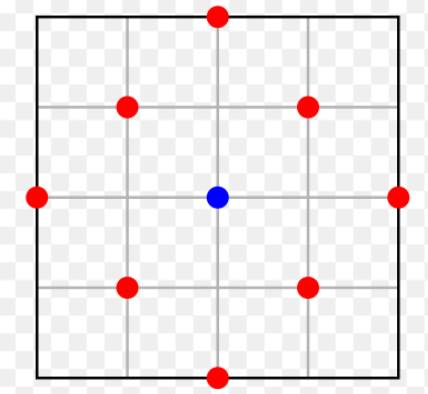
\includegraphics[scale=.25]{images/bar3}
\label{bar3}
\caption{   ബാറിലേക്കുള്ള വഴി }
\end{figure}

 \begin{figure}[H]
  \center
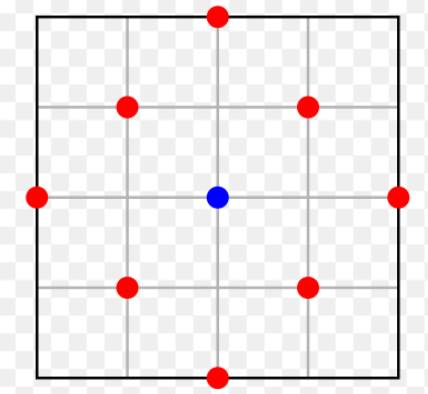
\includegraphics[scale=.25]{images/bar4}
\label{bar4}
\caption{   ബാറിലേക്കുള്ള വഴി }
\end{figure}


നിങ്ങൾ ചെസ് കളിച്ചിട്ടുണ്ടോ. ചെസിലെ റൂക്ക് നിങ്ങുന്നത്  മേൽ വിവരിച്ച ടാക്സികാബ്  പോലെയാണ് . ബിഷപ്പിന്റെ നീക്കങ്ങൾ 45° ചെരിച്ചുവച്ച ചെസ് ബോർഡിൽ ടാക്സി കാബ് രീതിയിലാണെന്ന് പറയാം. ഈ രീതിയിൽ ദൂരം അളക്കുന്ന രീതിയെ മാൻഹാട്ടൻ ഡിസ്റ്റൻസ് / സിറ്റി ബ്ലോക്ക് ഡിസ്റ്റൻസ് എന്നും വിളിക്കാറുണ്ട്.
          
          ബാറിലേക്കുള്ള ദൂരം ഏത് രീതിയിൽ അളക്കണമെന്ന് കോടതി പറയാത്തിടത്തോളം കാലം ബാർ സുഖമായി നടത്തത്താം.
 \begin{figure}[H]
  \center
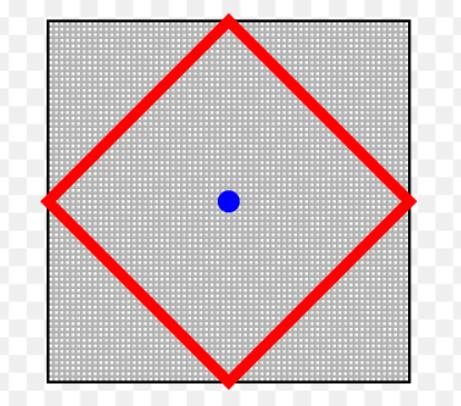
\includegraphics[scale=.25]{images/bar5}
\label{bar5}
\caption{   ബാറിലേക്കുള്ള വഴി }
\end{figure}


%\section{ബുക്ക് ബക്കറ്റും ഞാനും }
%നഷ്ടപ്പട്ടു പോയ ചില പുസ്തകങ്ങളെക്കുറിചു് ഓര്‍ക്കാന്‍ ഇടയായത് \#bookbucketchallenge ല്‍ ചിലര്‍ അവയെക്കുറിച്ചു് പരാമര്‍ശി ച്ച്പ്പൊളാണ്. അതില്‍ ഒന്നാണ് Ya. Peralman ന്റെ Mathematics can be fun. നാട്ടിന്‍ പുറത്തെ സാദ സ്കൂളിലെ കണക്ക് മാഷിന്റെ ചൂരലിനപ്പുറം ഗണിതം ഉണ്ട് എന്ന് മനസ്സിലാക്കി തന്നത് ഈ മനോഹരമായ പുസ്തകം ആണ്. പിന്നിട് എവിടെയോ കളഞ്ഞു പൊയി. ഒരിക്കല്‍ വീട്ടില്‍ മുഴുവന്‍ തിരഞ്ഞു. പക്ഷെ കിട്ടിയില്ല. ഇന്നലെ Navaneeth Krishnan S ഭൌതിക കൌതുകം അദ്ദേഹത്തിന്റെ ഇഷ്ടപുസ്തകപ്പട്ടികയില്‍ പെടുത്തിയത് കണ്ടപ്പൊള്‍ എനിക്ക് പെരല്‍മാനെ ഓര്‍മ  വന്നു. കുറെ തിരഞ്ഞപ്പൊള്‍ PDF കിട്ടി. കയ്യൊടെ പ്രിന്റ് എടുത്തു.
%
%\begin{figure}[htb]
%\begin{center}
%\includegraphics[height=2in,width=2in]{mf.jpg}
%\caption{ഗണിതം വിനോദത്തിന് }
%\end{center}
%\end{figure}

\section{ഇനിയും ചുട്ടെടുക്കാനുള്ള ദോശകൾ }
 \subsection{ ഫസി ലോജിക്കുള്ള  വാഷിങ് മെഷീൻ }

\subsection{ത്രികോണ സംഖ്യകൾ  }

\subsection{ ഒന്നുമുതൽ ആനന്തം വരെ കൂട്ടിയാൽ }

\subsection{എന്താണീ ഇന്റഗ്രേഷൻ }

\subsection{എന്താണ് മെഷീൻ ലേർണിംഗ് }

\subsection{ ന്യൂറൽ നെറ്വർക്കുകൾ }
\subsection{brachistochrone problem }

\section{Half Completed}

\subsection{നമ്പർ  കുടുംബങ്ങൾ }

\subsection{പ്രം നമ്പറുകളും  ഉലാം സ്പൈറലും }
\subsection{ട്രാൻസെൻഡെന്റല് നമ്പര് }

\subsection{ലിമിറ്റ്  കോൺവെർജൻസ് }

\subsection{കോണുകൾ അളക്കുന്നത് }

\subsection{കോംപ്ലക്സ് നമ്പറുകൾ}

\subsection{ടോപ്പോളജി }

\subsection{നമ്പർ തിയറി}  
 


\chapter{Music}
\section{ സുധീർ ഫട്കെ }
സുധീർ ഫട്കെ (1919-2002) മറാത്തി സിനിമാ ഗാനരംഗത്തെ അതികായനായിരുന്നു. ദീർഘകാലം RSS ഉമായി ചേർന്ന് പ്രവർത്തിച്ചിരുന്ന അദ്ദേഹം അവരുടെ സാംസ്കാരിക പ്രവർത്തനങ്ങളുടെ മുൻനിര പോരാളിയുമായിരുന്നു. 1955ൽ ഇദ്ദേഹത്തിന്റെ സംഗീത സംവിധാനത്തിൽ ഗീഥ് രാമായൺ എന്ന ഒരു റേഡിയോ പരമ്പര വരുകയുണ്ടായി. രാമായണ കഥ പാട്ടുകളിലുടെ പറയുന്ന ഈ പരമ്പര ഇപ്പോഴും മറാത്തികൾക്കിടയിൽ പോപ്പുലറാണ്. ഫട്കെ മാറാത്താ ഭാഷയിൽ ധാരാളം ഗാനങ്ങൾ പാട്ടുകയും സംവിധാനം ചെയ്യുകയും ചെയ്തിട്ടുണ്ട്. ചുരുക്കം ചില ഹിന്ദി ഗാനങ്ങളും. Bhabhi ki chudiyan എന്ന ചിത്രത്തിലെ ജോതി കലഷ് ചലകെ എന്ന മനോഹരഗാനം ചിട്ടപ്പെടുത്തിയത് സുധീർജിയാണ്. ഭൂപാളിയിലുള്ള ഈ പാട്ട് ലത പാടിയത് ഈ ലിങ്കിലുണ്ട്. മീനാകുമാരിയാണ് അഭിനയിച്ചിരിക്കുന്നത്.
\href{https://youtu.be/XiFSuo9qY9s}{ജോതി കലഷ് ചലകെ ലത പാടിയത്} 

%\url{https://youtu.be/XiFSuo9qY9s}
 \begin{figure}[H]
  \center
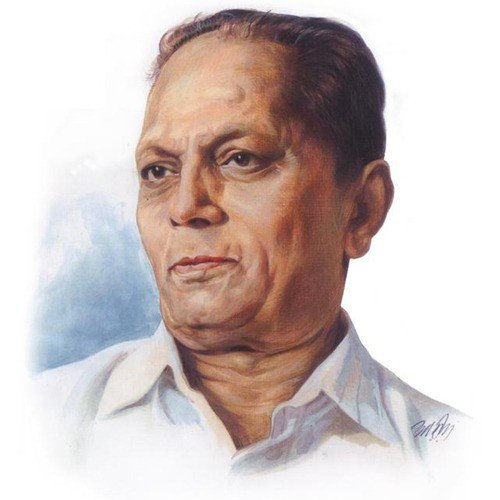
\includegraphics[scale=.25]{images/sudhir}
\label{sudhir}
\caption{ സുധീർ ഫട്കെ  }
\end{figure}
ഈ പാട്ട് സംഗീത സംവിധായകൻ തന്നെ പാടിയ ഒരപൂർവ്വ വിഡിയോ താഴെയുണ്ട്. സംഗീത സംവിധായകൻ പാട്ടിൽ ലയിച്ച് പാടുന്നതു കേൾക്കാൻ പ്രത്യേക സുഖമാണ്. (ബാബുരാജ് സുറുമയെഴുതിയ മിഴികളെ പാടുന്നതു കേട്ടിട്ടില്ലെ. അതുപോലെ
%\url{}
\href{https://youtu.be/FykYiZ2cOcw}{ജോതി കലഷ് ചലകെ സുധീർ ഫട്കെ പാടിയത്}


സുധീർജി യുടെ ഗീഥ് രാമയൺ ഭാഷയറിയില്ലെങ്കിലും കേൾക്കാൻ നല്ല രസമാണ്. \href{https://youtu.be/1yvZUmC34Q8}{ലിങ്ക് ഇവിടെ }
%\url{https://youtu.be/1yvZUmC34Q8}
\section{ ഓ ദുനിയാ കെ രഖ് വാലെ}
\begin{figure}[htb]
\begin{center}
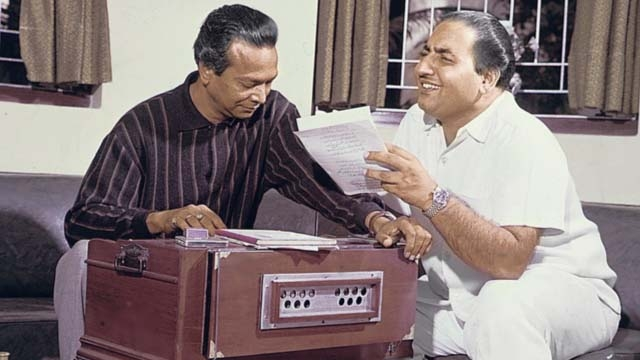
\includegraphics[scale=.4]{images/rafi.jpg}
%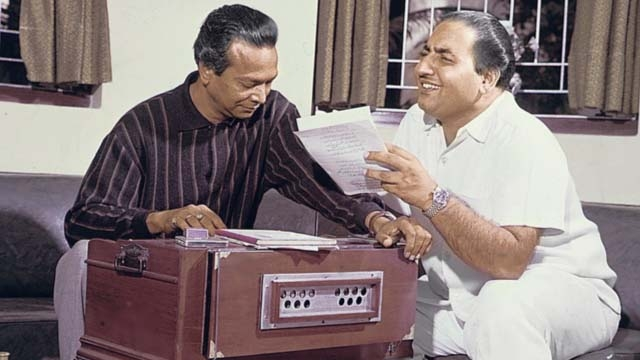
\includegraphics[ ]{images/rafi.jpg}
\caption{ റഫിയും നൗഷാദും  }
\end{center}
\end{figure}
റഫി യുടെ പാട്ടുകളിൽ ഏറ്റവും മനോഹരമായിട്ടുള്ള ഒന്നാണ് ബൈജു ബാവ്രയിലെ ഓ ദുനിയാ കെ രഖ് വാലെ. ദർബാർ രാഗത്തിലുള്ള ഈ ഗാനം നൗഷാദിന്റെ മാന്ത്രിക സംഗിതത്തിൽ 1952ലാണ് പുറത്തിറങ്ങിയത്. ഗായകനും സംഗീതസംവിധായകനും നന്നെ ചെറുപ്പം. താൻസെന്നെ പാടിത്തോൽപിച്ച ബൈജു ബാവ്രയുടെ കഥ ഒരു ഉത്തരേന്ത്യൽ ഐതീഹ്യമാണ്. മീനാകുമാരിയും ഭരത് ഭൂഷണും അഭിനയിച്ച ചിത്രത്തിന്റെ കഥ ഐതിഹ്വുമായി അത്ര സാമ്യം പുലർത്തുന്നില്ല
ബാല്യകാല സഖിയുടെ ജീവനറ്റ ശരീരം കണ്ട് ഭ്രാന്തനാകുന്ന ബൈജു പാടുന്ന പാട്ടാണ് ഓ ദുനിയാ കെ രഖ് വാലെ. (ഹിന്ദിയറിയാത്തവർക്കായി പാട്ടിന്റെ വിവർത്തനം ഇവിടുണ്ട്.
\href{http://www.ardhamy.com/song/o-duniya-ke-rakhwale}{പാട്ടിന്റെ ഇംഗ്ലീഷ് വിവർത്തനത്തിന്റെ ലിങ്ക്}

ഈ ഗാനം മുന്ന് വ്യത്യസ്ത സന്ദർഭങ്ങളിൽ റഫി പാടിയത് നെറ്റിൽ കിട്ടാനുണ്ട്. ഇവയോരോന്നും കേൾവിക്കാരന് വ്യത്യസ്തമായ അനുഭവം പകർന്നു തരും.

ഉദാഹരണത്തിന് സിനിമയിലെ ഒറിജിനൽ പാട്ട് ബൈജുവിന്റെ തിവ്രമായ ഹൃദയ വേദന വെളിവാക്കുന്ന ഒന്നാണ്. സ്റ്റുഡിയോയിൽ പല തവണ പരിശീലിച്ച് റികോർഡ് ചെയ്യപ്പെട്ട ഈ ആലാപനം തന്നെയാണ് കൂട്ടത്തിൽ ഏറ്റവും മികച്ചതും. ഇത് റകോഡ് ചെയ്ത് കഴിഞ്ഞ് കുറേ ദിവസത്തേക്ക് റഫീക്ക് പാടാൻ കഴിഞ്ഞില്ലെന്ന് പറയപ്പെടുന്നു.

\href{https://youtu.be/ReFDB8cexLg}{ഒറിജിനൽ പാട്ട്}

രണ്ടാമത്തെത് സംഗിത സംവിധായകൻ നൗഷാദിനൊപ്പം നടത്തുന്ന ലൈവ് പ്രോഗ്രാമിന്റെ റക്കോർഡിങ്ങാണ്. റഫി ഒരു പൂച്ചക്കുട്ടിയേപ്പോലെ സംവിധായകന്റെ വിരൽ ചലനങ്ങൾക്കൊത്ത് പാടുന്നു.

\href{https://youtu.be/Jlx1sJcYPI4}{1971ലെ ലൈവ് }

മുന്നാമത്തേത് റഫിയുടെ1979 ലെ ലണ്ടൻ പ്രോഗ്രാമിൽ നിന്നാണ്. ജനക്കൂട്ടത്തിന് വേണ്ടിയുള്ള മനോധർമ്മ സംഗിതമാണിത്. കരോക്കേയും ഇലക്ട്രോണിക് സംവിധാനങ്ങളുമില്ലാതെ റഫി എത്ര മനോഹരമായാണ് പാടുന്നത്.
ഗായകന്റെ കയ്യൊപ്പുള്ള ഈ ആലാപനങ്ങളെല്ലാം. കേൾവിക്കാരന് അമൃതു തന്നെ. ഇതാണ് ലിങ്ക്

\href{https://youtu.be/SpkbWeMDxok}{1979 ലെ ലണ്ടൻ പ്രോഗ്രാമിൽ}

വിഡിയോ അത്ര നന്നല്ല.അക്കാലത്ത് നല്ല ക്യാമറകളും റക്കോർഡിംങ്ങുമില്ലാത്തത് കൊണ്ട് നമുക്കാണ് നഷ്ടം. ഇത് കുറേക്കൂടി നല്ല റെക്കോർഡിങ്ങാണ്.

\href{https://youtu.be/7qKoPk4McLo}{വേറൊരു ലിങ്ക് }

ഈ പാട്ടിനെപ്പറ്റി \href{https://youtu.be/Nr6CrU1cqyA} {നൗഷാദ് ഇവിടെ പറയുന്നതു കൂടി കേൾക്കണം}.


\section{ഹിന്ദിപ്പാട്ടുകാരും മലയാളവും}
 

മലയാളം മാതൃഭാഷ അല്ലാത്തവർ മലയാളം പാട്ടുകൾ പാടുന്നത് ഇപ്പോൾ പുത്തരിയല്ല. ശ്രേയ ഘോഷാലും മറ്റും ഈ ഫീൽഡിൽ നിറഞ്ഞു നിൽക്കുകയാണ്. എന്നാൽ രണ്ടായിരത്തിനു മുമ്പ് അന്യഭാഷാ പാട്ടുകാർ പ്രത്യേകിച്ചും ഹിന്ദി ബംഗാളി പാട്ടുകാർ മലയാളത്തിൽ ചില മനോഹര ഗാനങ്ങളിൽ പാടിയിട്ടുണ്ട് മിക്ക പാട്ടുകളും ഹിറ്റായിരുന്നു. ഇവയിലുള്ള ഉച്ചാരണത്തിലുള്ള ചെറിയ പിഴവുകളൊക്കെ പാട്ടുകളുടെ മാറ്റു കൂട്ടിയിട്ടേ യുള്ളു. അത്തരത്തിലുള്ള ചില പാട്ടുകളെയും പാട്ടുകാരെയും പരിചയപ്പെടുത്തുന്നു.

1 മന്നാഡെ

മന്നാഡെ യുടേതായി രണ്ടു പാട്ടുകളാണുള്ളത്. ചെമ്മീനിലെ മാനസമൈനേ വരൂ എന്ന വിഖ്യാത ഗാനവും ജയചന്ദ്രനോടൊപ്പം നെല്ലിനു വേണ്ടിപ്പാടിയ ചമ്പാ ചമ്പാ എന്ന പാട്ടും. ഇതിൽ മാനസ മൈനേ മലയാളത്തിൽ എക്കാലവും ഓർമ്മിക്കപ്പെടുന്ന വിരഹഗാനമാണ്. ലിങ്കുകൾ താഴെ .

\href{https://youtu.be/W4FHG5baLOM}{മാനസമൈനേ വരൂ}

\href{https://youtu.be/aX1yQIwSLuw}{ചമ്പാ ചമ്പാ}

2 ലതാമങ്കേഷ്കർ

ലതയുടെ ഒരു പാട്ടേ യുള്ളു. നെല്ലിലെ കദളി ചെങ്കദളി. മലയാളത്തിനെന്നെന്നും ഓർമിക്കാൻ ഇതു മതി.

\href{https://youtu.be/Hh_Ne01I_UA}{കദളി ചെങ്കദളി}

3 ആഷാ ബോസ്ലെ

രവീന്ദ്ര ജയിനിന്റെ സ്വയംവര ശുഭദിന മംഗളങ്ങളാണ് ആഷ പാടിയ ഏക ഗാനം .
ആഷ ജിയുടെ പാട്ടിന്റെ ലിങ്കി താണ്‌. 

\href{https://youtu.be/3-jat5BG9MY}{സ്വയംവര ശുഭദിന}

4 ഹേമലത
ആഷയോടും ലതയോടും പ്രശസ്തയല്ലെങ്കിലും എഴുപതുകളിൽ ഹിന്ദിയിലെ നിറസാന്നിധ്യമായിരുന്നു ഹേമലത. ചിത് ചോറിൽ യേശുദാസിനൊപ്പം പാടിയ ജബ് ദിപ് ജലേആ കേട്ടിട്ടില്ലെ 1977ൽ രവിന്ദ്ര ജയിൻ ചിട്ടപ്പെടുത്തിയ സുജാതയിലെ ആശ്രിത വൽസലനെ എന്ന ഈ പാട്ട് കേൾക്കു.

\href{https://youtu.be/-p0tOi0uY-s}{ആശ്രിത വൽസലനെ}

5 തലത് മൊഹമുദ്.
ഗസൽ രാജകുമാരനായ തലത് മലയാളിക്ക് ഒരു പാട്ടേപടിത്തന്നിട്ടുള്ളു. ദ്വീപിലെ കടലേ നീലക്കടലേ എന്ന സുന്ദര ഗാനത്തിന്റെ ലിങ്കിവിടെ.

\href{https://youtu.be/iNKuno36Jtg}{കടലേ നീലക്കടലേ}

6)കിഷോർ കുമാർ
അയോധ്യയിൽ കിഷോർ ഒരു അടിപൊളിപ്പാട്ട് പാടിട്ടുണ്ട്.

\href{https://youtu.be/SUB3Q_i0px4}{കിഷോർ}

ഇവരെ കൂടാതെ ഉഷാ ഉതുപ്പ്, ഖണ്ഡശാല, പി ബി ശ്രിനിവാസ് തുടങ്ങി പലരും ഇവിടെ മുഖം കാണിച്ചിട്ടുണ്ട്. എസ് പി ബാലസുബ്രമണ്യം എസ് ജാനകിയുമൊക്കെ നമ്മുടെ സ്വന്തമായതിനാൽ അവരെ മലയാളികളായിത്തന്നെ പരിഗണിക്കണം.

\section{ മൊഴിമാറ്റിയ പാട്ടുകൾ}


വായനയുടെ കാര്യത്തിൽ ഞാനും മകൾ ലക്ഷ്മിയും തമ്മിൽ നല്ല സാമ്യമുണ്ട്. ചെറുതിലെതന്നെ പുസ്തകപ്പുഴുക്കളാണ് . രണ്ടാൾക്കും ക്ലാസിക് കൃതികൾ ഇഷ്ടമാണ് ത്രില്ലറുകളും. പലപ്പോഴും ഞങ്ങൾ തമ്മിൽ വായിച്ച പുസ്തകങ്ങളെ കുറിച്ച് ചർച്ച ചെയ്യാറുണ്ട്. എന്നാൽ പാട്ട് കേൾക്കുന്ന കാര്യത്തിൽ രണ്ടുപേരുടെയും അഭിരുചി വ്യത്യസ്തമാണ്. ലക്ഷ്മിക്ക് കുറച്ച് അടിപൊളി പാട്ടുകളാണ് ഇഷ്ടം. എനിക്ക് പഴയ ഹിന്ദി തമിഴ് മലയാളം പാട്ടുകളും. അതുകൊണ്ട് പാട്ടുകൾ വളരെ അപൂർവമായി മാത്രമേ ഞങ്ങളുടെ ചർച്ചകളിൽ വരാറുള്ളൂ. ഈയടുത്ത് ഒരു ദിവസം ജില്ല സിനിമയുടെ മലയാളം പതിപ്പിൽ വന്ന മൊഴി മാറ്റപ്പെട്ട പാട്ടുകൾ പരമ ബോറാണെന്ന് അവൾ പറയുന്നത് കേട്ടു. അങ്ങിനെയാണ് മൊഴി മാറ്റപ്പെട്ട പാട്ടുകളിലേക്ക് ചർച്ച എത്തിയത്. സൂര്യ ടി വി യും ബാഹുബലിയും കണ്ടുവളരുന്ന പുതുതലമുറയ്ക്ക് മൊഴി മാറി വരുന്ന ചിത്രങ്ങളോട് കുറച്ച് പുച്ഛം ഉണ്ട് . മിക്കവർക്കും ഹിന്ദിയും ഇംഗ്ലീഷും തമിഴും കേട്ടാൽ മനസ്സിലാകും. അതിനാൽ അവർ മൂലഭാഷ ചിത്രങ്ങൾ തന്നെയാണ് ഇഷ്ടപ്പെടുന്നത് വേറെ വഴിയൊന്നും ഇല്ലെങ്കിലെ  ഡബ്ബിങ് ചിത്രങ്ങൾ കാണൂ.

കേരളത്തിൽ സിനിമാ പ്രദർശനം തുടങ്ങിയ കാലം മുതൽ തന്നെ തമിഴ് ചിത്രങ്ങൾക്ക് നല്ല മാർക്കറ്റ് ഉണ്ടായിരുന്നു. എന്റെ അപ്പൻ ഒക്കെ പാലായിൽ വച്ച് പാതാളഭൈരവി കണ്ടിട്ടുണ്ട് എന്ന് ബഡായി പറയുന്നത് കേട്ടിട്ടുണ്ട്. എഴുപതുകളിലും എൺപതുകളിലും ധാരാളം തമിഴ് ഹിന്ദി ചിത്രങ്ങൾ മൂല ഭാഷയിൽത്തന്നെ കേരളത്തിൽ ഇറങ്ങിയിട്ടുണ്ട്. അപൂർവ്വംചില ഹിറ്റ് ചിത്രങ്ങൾ മലയാളത്തിലേക്ക് മൊഴിമാറ്റി റിലീസ് ചെയ്തിട്ടുണ്ട്. ശങ്കരാഭരണം പോലുള്ള ചില ചിത്രങ്ങൾ മൊഴി മാറി വന്നപ്പോഴും ഗാനങ്ങൾ മൂലഭാഷയിൽത്തന്നെ നിലനിന്നു. കവിതകൾ വിവർത്തനം ചെയ്യാൻ കവികൾക്കേപറ്റു എന്നിങ്ങനെ ഞാൻ തള്ളൽ തുടങ്ങി. കുറേ ഉദാഹരണങ്ങൾ പറഞ്ഞപ്പോഴേക്കും കക്ഷി സ്ഥലം കാലിയാക്കി.

മറ്റു ഭാഷകളിൽ നിന്ന് മൊഴി മാറി വന്ന ചിത്രങ്ങളിലെ മൊഴി മാറ്റപ്പെട്ട ചില മനോഹര ഗാനങ്ങൾ താഴെക്കൊടുക്കുന്നു. പല തിലും മൊഴിമാറ്റിയ കവിയുടെ ക്രാഫ്റ്റ് കാണാൻ കഴിയും. ഇത്തരം ഗാനങ്ങെളേപ്പറ്റി കൂടുതൽ അറിയാവുന്നവർ കമന്റായി ഒറിജിനലും മൊഴിമാറ്റിയതും ഇടുമല്ലോ.

(ട്യൂൺ അടിച്ച് മാറ്റിയ ഗാനങ്ങൾ ഇഷ്ടം പോലെയുണ്ട്. പങ്കജ് മല്ലിക്കിന്റെ പാട്ടൊക്കെ ഇവിടെ സുപ്പർ ഹിറ്റാവുന്നത് കണ്ടിട്ടുണ്ട്. ഞാനന്വോഷിക്കുന്നത് ആത്മാവ് നഷ്ടപ്പെടാതെ വിവർത്തനം ചെയ്ത വരികളാണ്. സലിൽ ചൗധരിയുടെ അനശ്വര ഗാനങ്ങൾക്ക് ട്യൂൺ മാത്രമേയുള്ളു, വരികൾക്ക്പ്രസക്തിയില്ല.)

1 1971 ൽ പുറത്തിറങ്ങിയ ജിവൻ മ്യുത്യ ധർമ്മേന്ദ്രയും രാഖിയും തകർത്തഭിനയിച്ച ത്രില്ലറാണ്. ഇത് ജീവിതസമരം എന്ന പേരിൽ മലയാളത്തിൽ മൊഴി മാറി വന്നു.

ജിൽ മിൽ സിതാരോം ആംഗൻ ഹോഗ എന്ന മനോഹരഗാനം പാടിയത് റഫിയും ലതയുമാണ്. പീ ഭാസ്കരൻ ഈ പാട്ടിനെ ചിന്നും വെൺ താരത്തിൻ ആനന്ദ വേള, ഏങ്ങും മലർശരൻ ആടുന്ന വേള എന്ന് മാറ്റിയെഴുതിയിട്ടുണ്ട്.
ഇതാണ് ലിങ്കുകൾ

ഹിന്ദി
\href{https://youtu.be/uex2GnRrqFU}{ജിൽ മിൽ സിതാരോം ആംഗൻ ഹോഗ }

മലയാളം
\href{https://youtu.be/JfDN6qEHvY8}{ചിന്നും വെൺ താരത്തിൻ ആനന്ദ വേള}

2 അവൾ ഒരു തൊടർക്കഥൈ സുജാത നടിച്ച ഹിറ്റ് പടമാണ് 1975ൽ ഇറങ്ങിയ ഈ ചിത്രത്തിൽ. കമാൽഹാസനൊക്കെ സൈഡ് റോളിലുണ്ട്. ഇതിലെ ഗാനങ്ങളെല്ലാം മനോഹരമമായി മൊഴി മാറ്റപ്പെട്ടവയാണ്.
എം എസ് വിശ്വനാഥന്റെ സംഗീതത്തിൽ വയലാർ മൊഴിമാറ്റിയ ദൈവം തന്നവീട് കേട്ടു നോക്കു.

മലയാളത്തിൽ  \href{https://youtu.be/dxcIZVxxyi4}{ദൈവം തന്നവീട്}

ഇതാണ് ഒറിജിനൽ.
\href{https://youtu.be/5_Zi5ROhjME}{ ദൈവം തന്ത വീട് }

ഇതിലെ തന്നെ കടവുൾ അമെത്തുവെക്കും മേടൈ മറ്റൊരു മനോഹര ഗാനമാണ്.
കമലിന്റെ മിമിക്രിയാണ് തിം .

ഒറിജിനൽ ഇതാണ്
\href{https://youtu.be/gJQ-grJjRgU}{കടവുൾ അമെത്തുവെക്കും മേടൈ}

മലയാളം ഇതും.
\href{https://youtu.be/5v2Yuqiw1Ng}{കളഭചുമരു  വെച്ചമേട് }

3) ഒരു തലൈ രാഗം ശങ്കറിന്റെ ആദ്യ തമിഴ് ചിത്രമാണ്. മലയാളത്തിലും തമിഴിലും ഒരേ സമയം സുപ്പർ ഹിറ്റുകളുമായിട്ടാണ് ശങ്കർ സിനിമയിൽ വന്നത്. ഇപ്പോൾ മഞ്ഞിൽ വിരിഞ്ഞ പൂക്കൾ കണ്ടാൽ കോമഡിയായിത്തോന്നും. പക്ഷെ ഒരു തലൈ രാഗം ഇപ്പോഴും കാണാവുന്ന പടമാണ്. ഇതിലെ പാട്ടുകൾ എല്ലാം വലിയ ഹിറ്റായിരുന്നു.
കടവുൾ വാഴും കോവിലിലെ ജയചന്ദ്രൻ പാടിയ ഹിറ്റ് ഗാനമാണ്.

\href{https://youtu.be/dAGruq3cOUU}{കടവുൾ വാഴും കോവിലിലെ}
ഇതിനെ മങ്കൊമ്പ് ഗോപാലകൃഷ്ണൻ ഈശ്വരന്റെ കോവിലിലാകെ എന്ന മനോഹര ഗാനമാക്കി.

\href{https://youtu.be/lYZkIL4iGHQ}{ഈശ്വരന്റെ കോവിലിലാകെ}

4) പ്രേമാഭിഷേകം
തെലുങ്കിൽ നിന്ന് തമിഴിലേക്ക് വാഴ്വേമായമായി റിമേക്ക് ചെയ്യപ്പെട്ട പടമാണിത്. അവിടുന്ന് മലയാളത്തിലെത്തിയപ്പോൾ വീണ്ടും പ്രേമാഭിഷേകമായി.
പുവച്ചൽ ഖാദർ മൊഴി മാറ്റിയ മഴക്കാല മേഘം കേട്ട് നോക്കു. കവിഞ്ഞർ വാലിയുടെ മഴൈക്കാലമേഘം ഇവിടുണ്ട്.
\href{https://youtu.be/6trDr3JOqcg}{മഴക്കാല മേഘം കേട്ട് }

5) സാഗരസംഗമം.
തെലുങ്ക് തമിഴ് വഴി വന്ന കമലിന്റെ ഹിറ്റ് ചിത്രമാണ് സാഗരസംഗമം.
Veturi Sundararama Murthy എഴുതിയ ഓം നമശിവായ തെലുങ്കിൽ കേട്ട് നോക്കു.

\href{https://youtu.be/m4RtS-TcbnY}{ഓം നമശിവായ }

തമിഴിൽ ഇത് കേൾക്കു.
\href{https://youtu.be/fFtTPz9h9jY}{ഓം നമശിവായ തമിഴിൽ }

ഹിന്ദോളത്തിലുള്ള ഈ മനോഹര ഗാനം മലയാളത്തിലെത്തിയപ്പോൾ

\href{https://youtu.be/wUnuMNyJ-yo}{ മലയാളത്തി ഓം നമശിവായ }
\section{പ്രേതങ്ങൾ ഉണരുമ്പോൾ } 
  Note on back ground score പ്രേതങ്ങൾ ഉണരുമ്പോൾ
\section{ഹിന്ദുസ്ഥാനി സംഗീതം കേൾക്കേണ്ടതെങ്ങിനെ ?}
   Summary of the course on Appreaciating hindustani Music by Prof. Milind Malshe (To be completed) 
\section{Note on Hemant kumar}
   
\section{note on guru dutt/geetha dutt}



\chapter{Technology}

\section{ റാസ്പ്ബെറി പൈ }

വെക്കേഷന് സ്കൂളിലെ ക്ലാസ് ഗവർമെന്റ് നിരോധിച്ചിരിക്കുകയാണല്ലോ. ഈ സമയത്ത് കുട്ടികളെക്കൊണ്ട് ചെയ്യിക്കാവുന്ന ഒരു ചെറിയ പ്രോജക്ടിനേ ക്കുറിച്ച് പറയാം. മുതിർന്നവർക്കും പരീക്ഷിക്കാം റാസ് പ്ബെറി പൈ എന്ന കുഞ്ഞൻ കസ്റ്റട്ടറിനേക്കുറിച്ച് കേട്ടിട്ടുണ്ടോ. ബ്രിട്ടണിലെ കുട്ടികളെ കമ്പ്യൂട്ടർ സയൻസിന്റെ അടിസ്ഥാന പാഠങ്ങൾ പഠിപ്പിക്കുക എന്ന ലക്ഷ്യത്തോടെ എബൻ അപ്ടൺ എന്നയാൾ തുടങ്ങിയ പ്രോജക്ട് ആണ് റാബ് പ്ബെറി പൈ. 2012ലാണ് പൈയുടെ ആദ്യ മോഡൽ ഇറങ്ങിയത്. തുടർന്ന് പൈ2 പൈ3 എന്നീ മോഡലുകളും വന്നു. 
ഹോബിയിസ്റ്റുകളും റോബോട്ടിക് കമ്മ്യൂണിറ്റിയും മറ്റും വ്യാപകമായി ഉപയോഗിക്കാൻ തുടങ്ങിയതോെടെ ലോകത്തെ പ്രധാന കമ്പ്യൂട്ടിങ്ങ് പ്രോജക്ടുകളിലൊന്നായി റാസ് പ്ബെറി പൈ മാറി. കട്ടികളെ കമ്പ്യൂട്ടിംഗ് അനുബന്ധ വിഷയങ്ങളും പഠിപ്പിക്കാൻ ഇതിലും നല്ല പ്ലാറ്റ്ഫോം വേറെയില്ല. ലിനക്സ് ഓപ്പറേറ്റിംഗ് സിസ്റ്റത്തിൽ പ്രവർത്തിക്കുന്നതിനായിട്ടാണ് പൈ ഡിസൈൻ ചെയ്തിട്ടുള്ളത്. വിൻഡോസ് 10 ന്റെ I0T വെർഷനും ഇതിലോടും .
പൈയുടെ ആദ്യ മോഡൽ മുതൽ ഞാൻ ഉപയോഗിച്ചിട്ടുണ്ട്. ആദ്യകാലത്ത് ഇന്ത്യയിൽ കിട്ടണമെങ്കിൽ വലിയ വില കൊടുക്കണമായിരുന്നു.എന്നാൽ ഇപ്പോൾ വളരെ കുറഞ്ഞ വിലയിൽ ഇന്ത്യയിലെവിടെയും പൈ ലഭ്യമാണ്. നിങ്ങൾക്ക് വാങ്ങാൻ ഉദ്ദേശമുണ്ടെങ്കിൽ തിരക്ക് ന്തപു ര ത്തുള്ള എലമെന്റ് സ് എന്ന സ്ഥാപനത്തിൽ പൈയും അനു ബന്ധ ഉപകരങ്ങളും ലഭ്യമാണ്.  http://elementzonline.com/ (എനിക്ക് ഇവരുമായി യാതൊരുബന്ധവുമില്ല. പലതവണ വാങ്ങിയിട്ടുണ്ട്. ഇവിടെ നിന്ന് ഓൺലൈനായും കിട്ടും.).ഏകദേശം 2900  രുപയാണ് .വില.

 \begin{figure}[H]
  \center
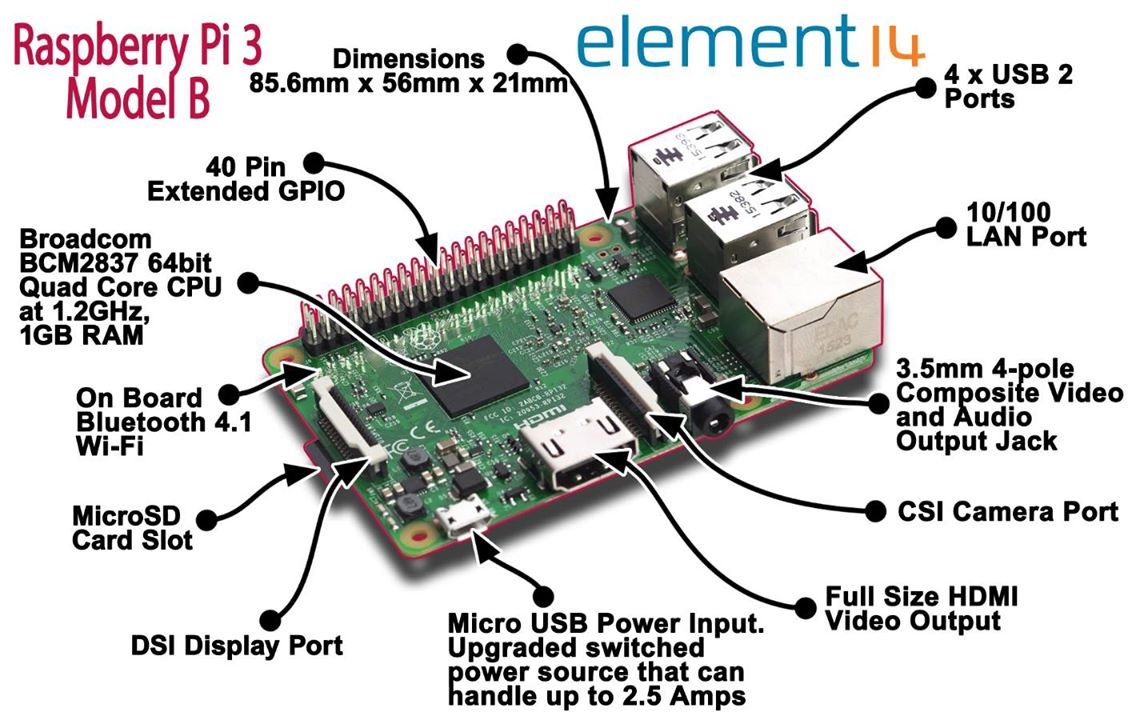
\includegraphics[scale=.25]{images/pi1}
\label{pi1}
\caption{    pi}
\end{figure}


നമുക്ക് ആദ്യം പൈ യെ പരിചയപ്പെടാം. ചിത്രം ഒന്നിൽ കാണുന്നതാണ് പൈ 3. ഇതിനെ ഉപയോഗയോഗ്യമാക്കണമെങ്കിൽ നിങ്ങൾക്ക് താഴെപ്പറയുന്ന സാധനങ്ങൾ കൂടി അവശ്യമായി വരും.
1) HDMI ഇൻപുട്ടുള്ള ടിവി. ഇത് മിക്കവാറും എല്ലാ LCD LED TV യിലും കാണും. ഈ ഇൻപുട്ട് ഉള്ള മോണിറ്റർ ആയാലും മതി. നിങ്ങളുടെ കയ്യിൽ സാധാരണ കമ്പുട്ടെർ മോണിറ്റർ ഉണ്ടെങ്കിൽ ചെറിയ ഒരു അഡാപ്റ്റർ ഉപയോഗിച്ച് അതിനെ HDMI മോണിറ്റർ ആക്കി മാറ്റാം. ചിത്രം രണ്ട് ഇത്തരത്തിലുള്ള അഡാപ്റ്ററിന്റെതാണ്.

 \begin{figure}[H]
  \center
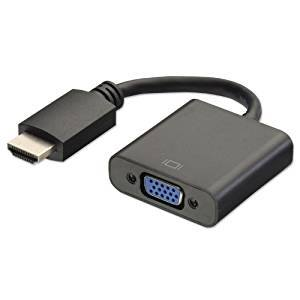
\includegraphics[scale=.25]{images/pi2}
\label{pi2}
\caption{    pi}
\end{figure}


2) 2.5 A കറണ്ട് തരാൻ കഴിവുള്ള മൊബൈൽ ചാർജർ. ഇത് പുതുതലമുറ ഫോണുകളുടെ ചാർജർ ആണ്. ഈ ത്രയും കറണ്ട് തരാൻ കഴിവുള്ള പവർ ബാങ്കായാലും മതി. പൈ അഞ്ചുവോൾട്ടിലാണ് പ്രവർത്തിക്കുന്നത്, അതിനാൽ പവർ ബാങ്ക് ഒരു യൂ പി എസ് പോലെ പ്രവർത്തിക്കും. 
3 ) 8GB കപ്പാസിറ്റിയുള്ള ഒരു മൈക്രൊ SD കാർഡ് .ക്ലാസ് 10 ആണെങ്കിൽ നന്ന്.
4) USB കീ ബോർഡ് മൗസ്. വയർലെസ് കീബോർഡ് ആണെങ്കിൽ നന്ന്.
5) Micro SD കാർഡ് റിഡർ (മൊബൈൽക്കടയിൽ 50 രൂപക്ക് കിട്ടും.)ചിത്രം 3

 \begin{figure}[H]
  \center
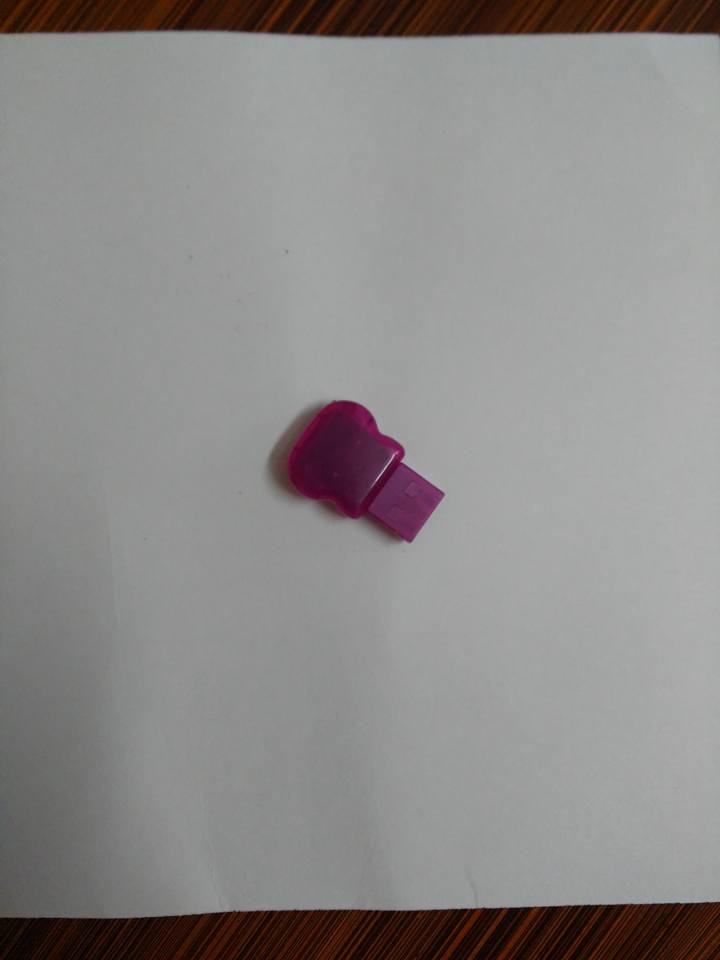
\includegraphics[scale=.25]{images/pi3}
\label{pi3}
\caption{    pi}
\end{figure}
card reader

റാസ് പ്ബെറി പൈ മൂന്നിൽ വൈഫൈ ബ്ലൂടൂത്ത് എന്നിവ ബിൽറ്റ് ഇൻ ആണ്. (പഴയ പൈ മോഡലുകളിൽ ഇവയില്ല.) പൈപ്രവർത്തിക്കുന്നത് arm പ്രോസസർ ഉപയോഗിച്ചാണ്. അതിനാൽ ഇതിന് വേണ്ടി ലിനക്സിന്റെ arm വെർഷനാണ് ഉപയോഗിക്കേണ്ടത്.
ഇത്രയും സാധനങ്ങൾ സംഘടിപ്പിച്ചു കഴിഞ്ഞാൽ നമുക്ക് പരീക്ഷണം തുടങ്ങാം.
ആദ്യമായി റാസ് പ്ബെറി പൈയുടെ സൈറ്റ് സന്ദർശിക്കുക. അവിടെ പൈയിൽ ഓടിക്കാൻ പറ്റുന്ന പലതരം ഓപ്പറേറ്റിംഗ് സിസ്റ്റങ്ങളുടെയും ഡൗൺലോഡ് ലിങ്ക് കൊടുത്തിട്ടുണ്ട്. തുടക്കക്കാർക്ക് നല്ലത് റാസ് പി യൻ  പിക്സൽ എന്ന വെർഷനാണ്. https://www.raspberrypi.org/downloa...
ഏകദേശം 4GB യുള്ള ഒരു zip ഫയൽ ആയിരിക്കും ഡൗൺലോഡ് ആവുക. (ഓപ്പറേറ്റിംഗ് സിസ്റ്റം ലോഡ് ചെയ്ത കാർഡുകൾ ഒൺലൈനിൽ ലഭ്യമാണ്).ഇതിനെ unzip ചെയ്യുക.
 അടുത്ത പണി ഈ ഫയലിനെ നമ്മുടെ മൈക്രോ എസ്ഡി കാർഡിൽ കോപ്പി ചെയ്യുക എന്നതാണ്. നാം ഡൗലോഡ്‌ ചെയ്ത് വെച്ചിരിക്കുന്ന ഫയൽ img എന്ന പ്രത്യേക ഫോർമാറ്റിലാണ്. അതിനാൽ ഇത് കാർഡിലേക്ക് എഴുതാൻ പ്രത്യേക സോഫ്റ്റ് വെയർ ഉപയോഗിക്കണം. പൈയുടെ സൈറ്റിൽ ഇത് എങ്ങിനെ ചെയ്യണമെന്ന് വിശദ മാ യി പ റ ഞ്ഞിട്ടുണ്ട്. 
ഇതിനാദ്യം etcher എന്ന സോഫ്റ്റ് വെയ ഇൻസ്റ്റാൾ ചെയ്യണം. ഇതാണ് ലിങ്ക്. ഇത് img ഫയലുകളെ കാർഡലാക്ക ന്നതിനുള്ള പ്രത്യേക സോഫ്റ്റ് വെയറാണ്. നിങ്ങളുടെ കാർഡ് റീഡറിൽ ഇട്ടതിന് ശേഷം യുഎസ്ബി പോർട്ടിൽ കുത്തുക.etcher തുറന്ന് നിങ്ങൾ ഡൗലോഡ് ചെയ്ത റാസ്ബിയൻ ഇമേജ് സെലക്ട് ചെയ്ത് കാർഡിലെഴുതുക. നിങ്ങളുടെ ഓപ്പറേറ്റിംഗ് സിസറ്റം തയ്യാർ. കാർഡ്സ് ലോട്ട് പൈയുടെ അടിഭാഗത്താണ്. ഓപ്പറേറ്റിംഗ് സിസ്റ്റം കയറ്റിയ കാർഡ് അതിന്റെ സ്ലോട്ടിൽ ഇടുക.
ഇനി HDMI കേബിൾ എടുത്ത് ഒരു തല TV യിലും മറുതല പൈയിലും പിടിപ്പിക്കണം TVക്ക് മിക്കവാറും പല ഇൻപുട്ടുകൾ കാണും. റിമോട്ടുപയോഗിച്ച് കൃത്യമായ ഇൻപുട്ട് തിരഞ്ഞെടുക്കണം. VGA HDMI അഡാപ്റ്റർ ഉപയോഗിച്ചാൽ ടിവിക്ക് പകരം മോണിറ്റർ ഉപയോഗിക്കാം.
പൈക്ക് നാല് യൂ എസ് ബി പോർട്ടുകളുണ്ട്. നിങ്ങളുടെ കൈവശമുള്ള കീബോർഡും മൗസും പൈയുടെ യു എസ് ബി പോർട്ടിൽ ഏതിലെങ്കിലും പിടിപ്പിക്കാം. ഇനി പൈക്ക് പവർ കൊടുക്കാം. എല്ലാ ശരിയായെങ്കിൽ പൈ ബൂട്ട് ആകും. ആദ്യം സ്ക്രീനിൽ മൂന്ന് റാസ് പ്ബെറി പഴങ്ങൾ പ്രത്യക്ഷപ്പെടും തുടർന്ന് ഗ്രാഫിക്കൽ ഇന്റർഫേസും.



 \begin{figure}[H]
  \center
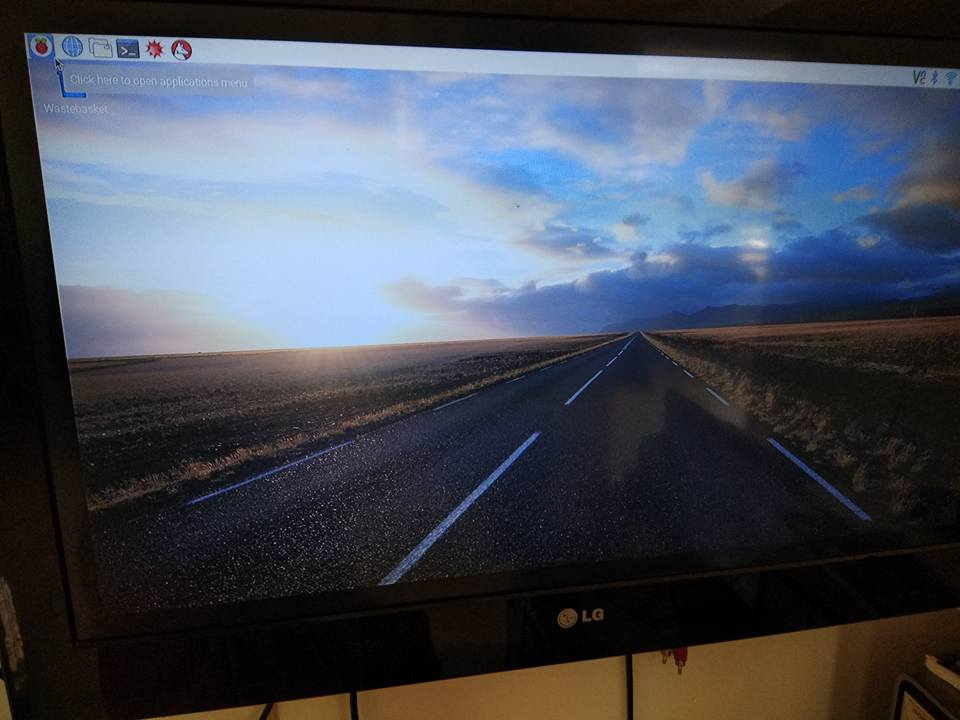
\includegraphics[scale=.25]{images/pi4}

\caption{  പിക്സിൽ എന്റെ ടിവിയിൽ   }
\label{pi4}
\end{figure}
അടുത്തതായി പൈയുടെ വൈ ഫൈ കോൺഫിഗർ ചെയ്യണം. ഇത് നമ്മൾ ഫോണിൽ വൈഫൈ കോൺഫിഗർ ചെയ്യുന്നത പോലെ തന്നെയാണ്. സ്ക്രീനിന്റെ മുകളിലത്തെ അരികിൽ വലത്തു വശത്തായി വൈ ഫൈ ഐ കോൺ കാണം.അതിൽ ക്ലിക്ക് ചെയ്ത് പാസ് വേർഡ് കൊടുത്താൽ മതി.
ഇനി പൈ കൊണ്ട് എന്തു ചെയ്യാം എന്ന് നോക്കാം. ആദ്യമായി പൈയുടെ ഇന്റർഫേസ് പരിചയപ്പെടുക. തുടർന്ന് ഇതിലുള്ള വിവിധ യൂട്ടിലിറ്റികൾ പരിശോധിക്കണം നിങ്ങൾക്ക് വേണമെങ്കിൽ ബ്രൗസുചെയ്യുന്നതിനും അത്യാവശ്യം ഓഫിസ് കാര്യങ്ങൾ നടത്തുന്ന തിരമുള്ള കമ്പ്യൂട്ടറായി ഇതിനെ ഉപയോഗിക്കാം.
പ്രോഗ്രാമിങ്ങിൽ താൽപര്യമുള്ളവർക്ക് ജാവാ പൈത്തൺ എന്നീ ഭാഷകൾ ലഭ്യമാണ്. ഗണിത ശാസ്ത്ര തൽപരർക്ക് മാത്തമാറ്റിക്ക കിട്ടും 
കുട്ടികൾക്ക് ചെറിയ ഹാർഡ് വെയർ പ്രോജക്ടുകളൊക്കെ ചെയ്തു നോക്കാൻ കഴിയും. മറ്റ് കമ്പ്യൂട്ടറുകളെ അപേക്ഷിച്ച് പൈ വ്യത്യസ്തമാക്കുന്നത് ഇവിടെയാണ്. മറ്റ് ഡിവൈസുകളെ നിയന്ത്രിക്കുന്നതിനും സെൻസറുകളെ കൂട്ടിയോജിപ്പിക്കന്നതിനും ധാരാളം പിന്നുകൾ ലഭ്യമാണ്.
ഇത് എങ്ങിനെ ഉപയോഗിക്കാമെന്ന് പിന്നീട് എഴുതാം.


   \section{മാങ്കാ ഗൈഡ്}
എന്റെ ചെറുപ്പക്കാലത്ത് കുട്ടികളുടെയിടയില്‍ ധാരാളം ചിത്രകഥകള്‍ പ്രചാരത്തിലുണ്ടായിരുന്നു. കണ്ണാടി വിശ്വനാഥന്‍ എന്നൊരാള്‍ ഇറക്കിയിരുന്ന CID മൂസ, പറക്കും ബെല്‍റ്റ് മഹേഷ്, ഇരുമ്പുകൈ മായാവി എന്നീ ചിത്രകഥാ പരമ്പരകള്‍ കുട്ടികള്‍ ഒളിച്ചും പാത്തും വായിച്ചിരുന്നു.ടിച്ചർ മാരെങ്ങാൻ  കണ്ടാൽ അടി ഉറപ്പായിരുന്നു. എങ്കിലും ക്ലാസ്സിലെ അണ്ടർ വേൾഡിൽ  ഇതിന്റെ വ്യാപാരം  പൊടിപൊടിച്ചിരുന്നു.   ഞാനൊക്കെ ഇരുമ്പുകൈ മായാവിയുടെ കട്ടഫാനായിരുന്നു. ഈ സമയത്ത് പത്രത്തിലും വാരികകളിലും ഫാന്റം മാന്‍ഡ്രേക്ക് തുടങ്ങിയ വിദേശ പരമ്പരകളുടെ വിവര്‍ത്തനവുമുണ്ടായിരുന്നു. ടെലിവിഷന്റെ വരവോടെയാണെന്ന് തോന്നുന്നു ഇവയൊക്കെ അപ്രത്യക്ഷമായത്.
 \begin{figure}[H]
  \center
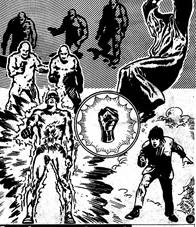
\includegraphics[scale=.55]{images/manga1}
\label{manga1}
\caption{   }
\end{figure}

     ചിത്രകഥകള്‍ എവിടെ കണ്ടാലും വായിക്കാന്‍ എനിക്ക് ഇഷ്ടമാണ്. മാങ്കാചിത്രകഥകളെ പരിചയപ്പെടുന്നത് IITയി വെച്ച് ഒരു സുഹൃത്തിന്റെ ബുക്ക് ഷെല്‍ഫില്‍ നിന്നാണ്. മാങ്കാ ഗൈഡ് ടു ഇലക്ട്രിസിറ്റിയാണ് ഇങ്ങനെ വായിച്ചത്.
           മാങ്കാ എന്നത് ജപ്പാന്‍കാരുടെ ചിത്രകഥാരചനാരീതിയാണ്. ഈ രീതി പഠിപ്പിക്കുന്ന പാഠശാലകള്‍ ജപ്പാനിലുണ്ട്. ധാരാളം വായനക്കാരും.

 \begin{figure}[H]
  \center
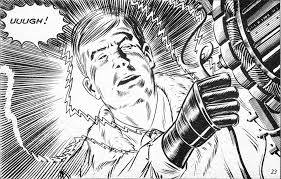
\includegraphics[scale=.5]{images/manga2}
\label{manga2}
\caption{   }
\end{figure}
   മാങ്കാ ഗൈഡ് ടു ഇലക്ട്രിസിറ്റി ഒരു ബെസ്റ്റ് സെല്ലര്‍ ആണ്. ചിത്രകഥയിലൂടെ വൈദ്യുതിയുടെ പ്രവര്‍ത്തനങ്ങള്‍ വിശദീകരിക്കുന്ന ഈ പുസ്തകം കുട്ടികള്‍ക്ക് സമ്മാനമായി കൊടുക്കാന്‍ അത്യുത്തമമാണ്.ഇലക്ട്രിസിറ്റിയുടെ അടിസ്ഥാന ആശയങ്ങള്‍ വിവരിക്കുന്ന ഇതിന്റെ ഏകദേശ രൂപം ഇങ്ങിനെയാണ്.
 \begin{figure}[H]
  \center
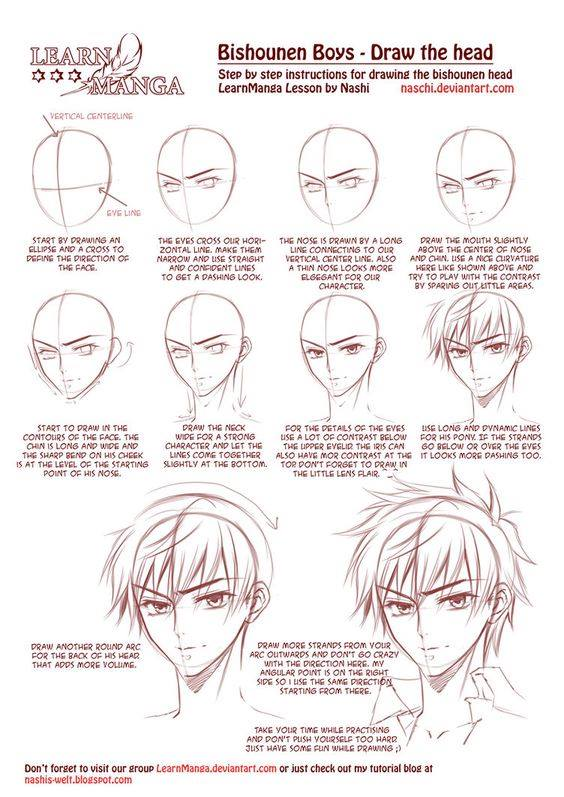
\includegraphics[scale=.25]{images/manga3}
\label{manga3}
\caption{   }
\end{figure}
    റെറെക്കൊ ഇലക്ടോപ്യ എന്ന രാജ്യത്തെ ഹൈസ്കൂള്‍ വിദ്യാര്‍ത്ഥിനിയാണ്. കക്ഷി ഇലക്ട്രിസിറ്റി പരീക്ഷയില്‍ തോറ്റു. തോറ്റകുട്ടികള്‍ വേനലവധിക്ക് പഠിച്ച് 'സെ' പരീക്ഷ എഴുതണം എന്ന നിയമം പണ്ടേ നടപ്പുള്ള രാജ്യമാണ് ഇലക്ടോപ്യ. റെറെക്കൊയുടെ അവധിക്കാല പഠനം നടക്കുന്നത് ഭൂമിയിലാണ്. ഭൂമിയില്‍ നിന്ന് ഇലക്ടോപ്യയിലേക്ക് പോകുന്നതിനും വരുന്നതിനും യോണോസൂക്ക് എന്ന സംവിധാനം ഉണ്ട്. റെറെക്കൊ ടോക്യോ യൂണിവേഴ്സിറ്റിയില്‍ റിസര്‍ച് ചെയ്യുന്ന ഹിക്കാറുവിനെ കണ്ടുമുട്ടുന്നു. ഹിക്കാറു ഇലക്ട്രിസിറ്റിയുടെ അടിസ്ഥാനപാഠങ്ങള്‍ അവളെ പഠിപ്പിക്കുന്നു. ചിത്രകഥയില്‍ ഹിക്കാറുവിന്റെ ഇലക്ട്രിസിറ്റി പാഠങ്ങള്‍ വിശദമായി ഉണ്ട്. 
 \begin{figure}[H]
  \center
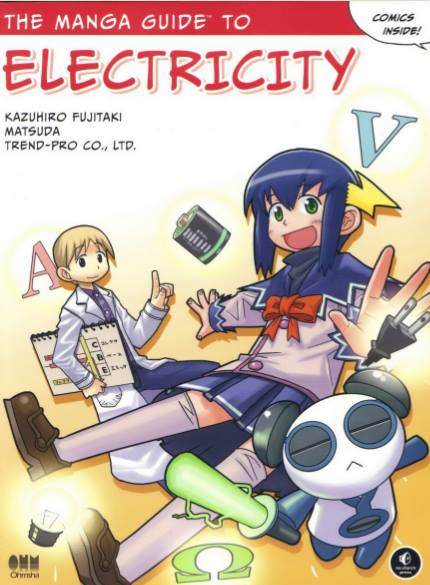
\includegraphics[scale=.25]{images/manga4}
\label{manga4}
\caption{   }
\end{figure}
ഹികാറു വിന്റെ പാഠങ്ങൾ

  വേനലവധി കഴിഞ്ഞ് റെറെക്കൊ തിരിച്ചുപോകുമ്പോഴേക്കും അവള്‍ എല്ലാ പാഠങ്ങളും പഠിച്ചിരുന്നു. ഒരു വര്‍ഷത്തിന് ശേഷം ഹിക്കാറു ഒരു ബസ്സ്റ്റോപ്പില്‍ നില്‍ക്കുകയായിരുന്നു. പെട്ടെന്ന് ഒരു മിന്നല്‍ അതാ റെറെക്കൊ വീണ്ടും ഭുമിയില്‍ തിരിച്ചെത്തി. താന്‍ പരീക്ഷ പാസായെന്നും ഇനി മുതല്‍ ടോക്യോ യൂണിവേഴ്സിറ്റിയില്‍ റിസര്‍ച്ച് ചെയ്യാനാണ് വന്നിരിക്കുന്നതെന്നും അവള്‍ പറയുന്നതോടെ കഥ തീരുന്നു. നോ സ്റ്റാര്‍ച്ച് പ്രസ് പ്രസിദ്ധീകരിച്ചിട്ടുള്ള ഈ പുസ്തകം അമസോണില്‍ ലഭ്യമാണ്  (http://www.amazon.in/Manga-Guide-El...   ) archive.org യിൽ പി ഡി എഫ് പോലും കിട്ടും. https://archive.org/details/TheMang...   

 \begin{figure}[H]
  \center
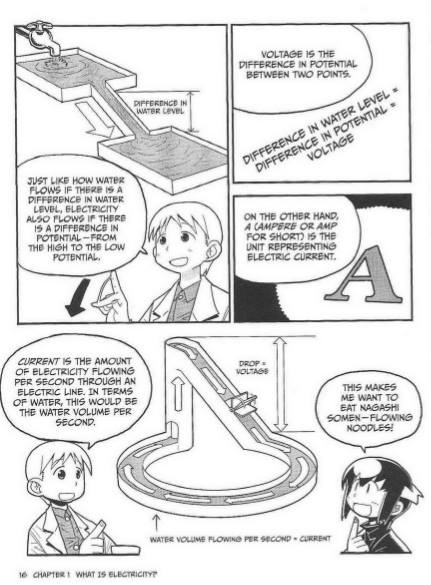
\includegraphics[scale=.25]{images/manga5}
\label{manga5}
\caption{   }
\end{figure}
    നോ സ്റ്റാര്‍ച്ച് പ്രസിന് ഈ സീരിസില്‍ 41 പുസ്തകങ്ങള്‍ ഉണ്ട്. വിവിധ വിഷയങ്ങളെ ചിത്ര കഥകളിലൂടെ പരിചയ പെടാൻ  പറ്റും  ചിലതൊക്കെ ഞാന്‍ വായിച്ചിട്ടുണ്ട്.ഇതൊക്കെ മലയാളംത്തിൽ   പരിഭാഷപ്പെടുത്തി കിട്ടിയാൽ നന്നായിരുന്നു.   
   
    \section{SDR}
    ഇലക്ട്രോണിക്സ്, കമ്പ്യട്ടർ, കമ്മ്യൂണിക്കേഷൻ എന്നിയയിൽ താൽപര്യമുള്ളവർക്ക് ചെയ്യാൻ പറ്റുന്ന ഒരു ഹോബി പ്രോജക്ട് പരിചയപ്പെടുത്താം. സംഗതി സോഫ്റ്റ് വെയർ ഡിഫൈൻഡ് റേഡിയോ ആണ്. സാധാരണ നാം കാണുന്ന റേഡിയോ ഒക്കെത്തന്നെ അനലോഗ് റിസപ്ഷനാണ് നടത്തുന്നത്. റേഡിയോ തരംഗങ്ങളെ സ്വീകരിച്ച് അതിൽ നിന്ന് ശബ്ദതരംഗങ്ങളെ വേർതിരിച്ച് നമ്മെ കേൾപ്പിക്കകയാണ് ഇവയുടെ ജോലി. 
    
    നാം നിത്യേന കാണുന്ന റേഡിയോയിൽ അനലോഗ് സിഗ്നൽ പ്രോസസിംഗ് ആണ് ഉപയോഗിക്കുന്നത്. ഈ രീതിയിൽ നമുക്ക് ആവശ്യമായ സിഗ്നലിനെ അനാവശ്യ നോയിസിൽ നിന്ന് വേർതിരിക്കുന്നതിനുള്ള കഴിവ് പരിമിതമാണ്‌. ഇതു കൊണ്ടാണ് ഇടിമിന്നൽ വരുമ്പോഴും സ്വിച്ചിടുമ്പോഴും റേഡിയോയിൽ പറ പറ ശബ്ദം കേൾക്കുന്നത്. സോഫ് റ്റ് വെയർ ഡിഫൈൻഡ് റേഡിയോ ഇലക്ട്രോമാഗ്നറ്റിക് തരംഗങ്ങളെ സ്വീകരിച്ച് അന ലോഗ് ഡിജിറ്റൽ കൺവെർഷൻ നടത്തി സിഗ്നലിനെ ഡിജിറ്റൽ രൂപത്തിലാക്കും. തുടർന്ന് നമുക്കാവശ്യ മായ ഇൻഫോർമേഷൻ വേർതിരിക്കുക, അതിന്റെ രൂപവും ഭാവവും മാറ്റുക തടങ്ങിയ ജോലികൾ കമ്പ്യൂട്ടിംഗ് ടെക്നിക്കുകൾ ഉപയോഗിച്ച് നടത്തും. അന ലോഗ് സംവിധാനത്തെക്കാൾ വളരെ കാര്യക്ഷമമായി സിഗ്നൽ പ്രോസസിംഗ് നടത്താനാകും എന്നതാണ് ഇവയുടെ മെച്ചം. സോഫ്റ്റ് വെയർ ഡിഫൈൻഡ് റേഡിയോ നിങ്ങളുടെ മൊബൈലിലൊക്കെയുണ്ട്. 
    
    ഇനി നമുക്ക്‌ പരീക്ഷണത്തിലേക്ക് കടക്കാം. RTLSDRഡോങ്കിൾ ഒരണ്ണം സംഘടിപ്പിക്കുകയാണ് ആദ്യം ചെയ്യേണ്ടത്. ഈ ഡോങ്കിളുകൾ ഡിജിറ്റൽ വിഡിയോ ബ്രോഡ്കാസ്റ്റ് (DVB - T) റിസീവർ എന്ന പേരിലാണ് മാർക്കറ്റിൽ കാണുക. ഡി വി ബി നമ്മുടെ നാട്ടിൽ പ്രചാരത്തിലില്ലാത്തതിനാൽ ലോക്കൽ കടയിൽ കിട്ടിയെന്നു വരില്ല. അലി എക്സ്പ്രസിലും ഇബേയിയും 10 ഡോളറിൽ താഴെ വിലയ്ക്ക് ഇവകിട്ടും. 24 മെഗാഹെർട്ട്സ് മുതൽ 1850 മെഗാഹെർട്ട്സ് വരെയുള്ള ഏത് ഫ്രീക്വൻസിയിലും ഇവയെ ട്യൂൺ ചെയ്യാം. ഇത് വളരെ വലിയ ഒരു റേഞ്ച് ആണ്. ഒരു മാതിരി കമ്മ്യൂണിക്കേഷൻ ചാനലുകളൊക്കെ ഈ റേഞ്ചിൽ വരും. RTLഡോങ്കിൾ വിൻഡോസിലും ലിനക്സിലും ആൻഡ്രോയിഡിലും പ്രവർത്തിക്കും. വിൻഡോസിൽ SDR  എന്ന സോഫ്റ്റ് വെയർ ഉപയോഗിക്കാം. ലിനക്സിൽ നിറയെ ഓപ്ഷൻസ് ഉണ്ട്.ഈ സോഫ്റ്റ് വെയറുകൾ എല്ലാം വിവിധ മോഡുലേഷൻ സ്കീമുകൾ ഡി കോഡ് ചെയ്യും. നിങ്ങൾക്ക് മേൽ പറഞ്ഞ റേഞ്ചിലുള്ള ഏത് ഫ്രീക്വൻസിയിലും നടക്കുന്ന കമ്യൂണിക്കേഷൻ കേൾക്കാൻ പറ്റും ( കേട്ടിട്ട് പോലിസിന്റെ ഇടി കിട്ടിയാൽ ഞാനുത്തരവാദിയല്ല) . ഇത്തിരി പരിശ്രമിച്ചാൽ എയർക്രാഫ്റ്റ് ,കാലാവസ്ഥ സംബന്ധിച്ച വിവരങ്ങൾ കേൾക്കാൻ പറ്റും.
    
     ആദ്യമായി പരീക്ഷിക്കുന്നവർ FM റേഡിയോ, ദൂരദർശൻ, ഹാം റേഡിയോ എന്നിവ ട്യൂൺ ചെയ്ത് നോക്കുക.a ഒരു ഹോബി എന്ന നിലയിൽ ചെയ്യാവുന്ന പരീക്ഷണങ്ങളിൽ ചിലത് ഇവയാണ്. 1) ഡോങ്കിളിന് എക്റ്റേണൽ ആന്റി ന പിടിപ്പിക്കുക. 2) ഷോർട്ട് വേവ് സിഗ്നൽ (24 mhzൽ താഴെ) കേൾക്കുന്നതിന് ഒരു ചെറിയ കൺവെർട്ടർ നിർമ്മിക്കുക. 3) ഇ ന്റർനാഷണൽ സ്പേസ് സ്റ്റേഷൻ കേൾക്കുക 4) ഈ ഡോങ്കിൾ റാസ്പ്ബെറി പൈ പോലെയുള്ള കുഞ്ഞൻ കമ്പ്യൂട്ടറുമായി കണക്ട് ചെയ്ത് ഒരു പോർട്ടബിൾ റേഡിയോ ഉണ്ടാക്കുക ഇലക്ടോണിക്സ് വിദ്യാർത്ഥികൾക്ക് അവരുടെ കമ്മ്യൂണിക്കേഷൻലാബ്. ഡി എസ് പി ലാബ് തുങ്ങിയവയിൽ നടത്തുന്ന പരീക്ഷണങ്ങൾ എല്ലാം ഈ ഡോങ്കിളിൽ നിന്ന് കിട്ടുന്ന റോ ഡാറ്റാ ഉപയോഗിച്ച് ചെയ്യാം. ഐ ഐ ടി ബോംബേയിലെ കമ്യൂണിക്കേഷൻലാബ്, എം ഐ ടി സിഗ്നൽ പ്രോസസിംഗ് ലാബ് എന്നിവയുടെ ലിങ്ക് കണ്ടു പിടിച്ച് നോക്കായാൽ കുടുതൽ വിവരം കിട്ടും. ഇതിനുമപ്പുറത്തേക്ക് പോകേണ്ടവർക്ക് ഗ്നൂ റേഡിയോയിൽ കൈവെക്കാം.  താഴെ എന്റെ കയ്യിലുള്ള ഡോങ്കിൾ കാണിച്ചിരിക്കുന്നു. റാസ് പ്ബെറി പൈയിൽ പിടിപ്പിച്ചാണ് ഞാൻ ഉപയോഗിക്കുന്നത്. കൂടുതൽ വിവരങ്ങൾക്ക് ഈ സൈറ്റ് നോക്കാം.
    % https://rtlsdr.org
    
     \section{ Make}
  %  Ranjith Antony ഇന്നിട്ട പോസ്റ്റിൽ വേറിട്ടു നിൽക്കുന്ന ഒരു റെസ്യമെ എഴുതേണ്ടതെങ്ങിനെ എന്ന് വിശദമായി എഴുതിയിട്ടുണ്ട്. റസ്യമെയിൽ സ്വന്തമായി ചെയ്ത ഹോബി പ്രോജക്ടുകളേക്കുറിച്ച് എഴുതാൻ അദ്ദേഹം അവശ്യപ്പെടുന്നുണ്ട്.
    This is to be corrected
     സ്വന്തമായി എന്തെങ്കിലും  ഹോബി പ്രോജക്ടുകളേക്കുറിച്ച് ചെയ്യണമെന്ന് ആഗ്രഹിക്കുന്ന നിരവധിയാളുകളുണ്ട്. പക്ഷെ പലർക്കും എവിടെ തുടങ്ങണം എന്ത് ചെയ്യാൻ പറ്റും എന്തൊക്കെ ടൂൾ സ് വേണം എന്നതിനേക്കുറിച്ചൊന്നും ഒരു ധാരണയുമുണ്ടാവില്ല. എഞ്ചിനിയറിംഗ് കോളേജിൽ പഠിച്ചാൽ മിക്കവാറും ഉള്ള ധാരണ കൂടി ഇല്ലാതാകും.പരീക്ഷ പാസാകാം പക്ഷെ പണി പഠിക്കില്ല. ഇലക്' ട്രോണിക്സ് ഹോബി പ്രോജക്ടുകൾ ചെയ്യുന്നതിനുള്ള ചില ടിപ്പുകൾ തരാം. ആദ്യമായി ഇലക്ട്രോണിക് കമ്പോണന്റുകളേയും അനുബന്ധ ഉപകരണങ്ങളേയും പരിചയപ്പെടണം. ഇതിന് ഞാൻ റെക്കമെന്റ് ചെയ്യുന്നത് MAKE മാഗസിന്റെ ഇലക്ട്രോണിക്സ് എന്ന പുസ്തകമാണ്.ഇതിന്റെ സബ് ഹെഡിംഗ്‌ ലേ ർ ണിംഗ്‌ ബൈ ഡിസ്കവറി എന്നാണ്.
     
      ഓരോ ചാപ്റ്ററിലും സാധനങ്ങൾ കണ്ടു പിടിച്ചു വരെക്കുറിച്ചൊക്കെ രസകരമായി എഴുതിയിട്ടുണ്ട്. നോവൽ പോലെ വായിക്കാം.(ലിങ്കും സാമ്പിൾ ചാപ്റ്ററും താഴെ. ചിന്തിക്കുന്നവർക്ക് ടോറന്റു തപ്പാം). തുടക്കക്കാർക്കു വേണ്ട എല്ലാ വിവരങ്ങളും ഇതിലുണ്ട്. ആദ്യത്തെ കുറെ ചാപ്റ്ററുകൾ മനസ്സിരുത്തി വായിക്കുക. നിങ്ങളെ ഈ പുസ്തകം ആകർഷിക്കുന്നില്ലെങ്കിൽ ഇലക്ട്രോണിക്സ് പ്രോജക്ട് റെസ്യൂമെ യിൽ എഴുതിയിട്ട് വലിയ ഫലമുണ്ടാകില്ല.
      
       1) വലിയ പ്രോജക്ടുകൾ ചെയ്യാൻ തുടക്കത്തിലേ ശ്രമിക്കരുത്. ചെറിയ ഒരു സർക്യകട്ടോ മെക്കാനിക്കൽ അസംബ്ലിയോ ഒക്കെ ആദ്യം പരീക്ഷിക്കണം. മുകളിൽ പറഞ്ഞിരിക്കുന്ന പുസ്തകത്തിലെ സർക്യൂട്ടുകൾ പരീക്ഷിക്കാം 
       
       2) നമുക്ക് വേണ്ട അത്യാവശ്യംടൂൾസ് സംഘടിപ്പിക്കണം. ഒരു സ്ക്രു ഡ്രൈവർ സെറ്റ് .വയർ സ്ട്രിപ്പർ കട്ടിംഗ് പ്ലെയർ, സോൾഡറിം ഗ് അയേൺ, വില കുറഞ്ഞ ഒരു മൾട്ടിമീറ്റർ എന്നിവ നിർബന്ധമായും വേണം. ഇതെല്ലാം അമസോണിലും ഇ ബേയിലും കിട്ടും. 
       
       3) നിങ്ങൾ ചെയ്യാനുദ്ദേശിക്കുന്ന പ്രോജക്ട് പലരും ചെയ്തിട്ടുണ്ടാകും. അതിന്റെ വിഡിയോ ഉണ്ടെങ്കിൽ നിർബന്ധമായും കണ്ടിരിക്കുക. തുടക്കക്കാർ വർക്ക് ചെയ്യും എന്ന് ഉറപ്പുള്ള പ്രോജക്ടുകൾ ഡ്യ പ്ലിക്കേറ്റ് ചെയ്താണ് പഠനം തുടങ്ങേണ്ടത്. 
       
       4) മിക്കവാറും പ്രോജക്ടുകൾ ചെറിയPC B യി ലൊക്കെയാവും ചെയ്യുക. ജനറൽ പർപ്പസ് PC Bകുറച്ച് സംഘടിപ്പിച്ച് സോൾഡറിംഗ് അത്യാവശ്യം പ്രാക്ടീസ് ചെയ്യണം. വൃത്തിയായി സോൾഡർ ചെയ്യാനാകും എന്ന് ഉറപ്പാക്കിയിട്ടേ പ്രോജക്ടിന്റെ അസംബ്ലി തുടങ്ങാവു. PC Bസ്വന്തമായിട്ടുണ്ടാക്കുന്നതെങ്ങിനെ എന്ന് അടുത്ത പോസ്റ്റിൽ എഴുതാം.
       
        5) നിങ്ങൾ ഉണ്ടാക്കിയ സർക്യൂട്ട് പവർ ചെയ്യുന്നതിന് മുൻപ് ഒന്നോ രണ്ടോ തവണ പരിശോധിക്കണം. 
        
        6) ആദ്യം ചെയ്യുന്ന പ്രോജക്ട് മിക്കവാറും വർക്ക് ചെയ്യില്ല. അതു കൊണ്ട് തളരരുത്. തുടക്കക്കാർ മിക്കവാറും വയറിംഗ് തെറ്റിക്കും. സോൾഡർ ചെയ്ത സർക്യട്ട് ഒറിജിനൽ ഡയഗ്രവുമായി ഒത്തു നോക്കണം. മൾട്ടിമീറ്റർ ഉപയോഗിച്ച് സർക്യൂട്ടിലെ വോൾട്ടേജ്, കറൻറ് എന്നിവ പരിശോധിക്കണം. 
        
        7) സർക്യൂട്ട് വർക്ക് ചെയ്യുന്നില്ലെങ്കിൽ, നിങ്ങൾ ബാഹുബലിയോ മറ്റോ പോയി കണ്ടിട്ട് വരുക. വീണ്ടും സർക്യട്ട് ശരിയാക്കാൻ നോക്കുക. 
        
        8) ഒന്നു രണ്ട് ചെറിയ പ്രോജക്ടുകൾ ചെയ്ത് കോൺഫിഡൻസ് ആയാൽ കുറേക്കൂടി വലിയതിലേക്ക് കടക്കാം
    % Make: Electronics https://www.amazon.in/dp/9352132300/ref=cm_sw_r_cp_apa_i_AKnbzbJG6AJM0 https://www.makershed.com/products/make-electronics-1ed-pdf
    
   
    
    \section{Voting Machine}
    ഇലക്ട്രോണിക് വോട്ടിംഗ് മെഷീനെ കുറിച്ച് Totto Chan ന്റെ പോസ്റ്റിൽ ഞാൻ ഇട്ട കമന്റ് ഇവിടെ പോസ്റ്റുന്നു. സോഫ്റ്റ് വെയർ / hard ware എന്നിവ ഓപ്പൺ അല്ലാത്തിടത്തോളം കാലം EVM മാനിപുലേറ്റ് ചെയ്യാൻ സാധ്യതയുണ്ട്. ഇലക്ഷനിലെ വിവിധ ഘട്ടങ്ങളിൽ പങ്കെടുത്ത അനുഭവം വെച്ച് എന്റെ ചില നിരീക്ഷണങ്ങൾ താഴെ കൊടുക്കുന്നു.
    
     1) EVM massive ആയി നിർമിക്കപ്പെടുന്ന ഒരു ഉപകരണമാണ്. 16 സ്ഥാനാർത്ഥികളെ ഉൾക്കൊള്ളാവുന്ന ഒരു ജനറൽ പർപ്പസ് മെഷീൻ ആണ് ഇപ്പോൾ ഉപയോഗത്തിലുള്ളത്. ഒരോമെഷിനും ഏതൊക്കെ മണ്ഡലത്തിലാകും ഉപയോഗിക്കുക എന്നത് ഉൽപാദന സമയത്ത് നിശ്ചയിക്കാനാവില്ല.വ്യാപകമായി മാനി പുലേറ്റ് ചെയ്യണമെങ്കിൽ ചിപ്പ് ലെവലിൽ സോഫ്റ്റ് വെയറിൽ ആകും നടക്കുക.
     
      2 ഇത്തരം മാനിപുലേഷൻ ആക്ടിവേറ്റ് ചെയ്യുന്നതിന് ഏതെങ്കിലും തരത്തിലുള്ള റിമോട്ട് കൺട്രോളോ കി കോംബിനേഷനോ ഉപയോഗിക്കണം. ഇതിന് രണ്ടിനും സാധ്യത വോട്ടെടുപ്പിനും എണ്ണലിനും ഇടയിലാണ്. ഇത് ചെയ്യണമെങ്കിൽത്തന്നെ പലർ ചേർന്നേ ചെയ്യാനാകൂ . ഒരു സംസ്ഥാനത്ത് നൂറു കണക്കിന് കൗണ്ടിങ്ങ് സ്റ്റേഷൻ ഉണ്ടാകും.അവിടെയൊക്കെ പോയി മാനി പുലേഷൻ പുറം ലോകമറിയാതെ ചെയ്യാൻ എളുപ്പമാണോ? ഉപയോഗിക്കുന്ന സമയത്തു നെറ്റ്വർകിൽ ഇവയെ ഘടിപ്പിക്കുന്നതേയില്ല. 
      
      3 ഓരോ മണ്ഡലത്തിലും സ്ഥാനാർത്ഥിപ്പട്ടിക അക്ഷരമാലക്രമത്തിലാണ്. മെഷിന് താമരയും കൈപ്പത്തിയും തമ്മിൽ തിരിച്ചറിയാനാകില്ല. അത് നോക്കുന്നത് ഏത് ബട്ടനാണ് വോട്ടർ ഞെക്കിയത് എന്നതു മാത്രം. ഏതു ബട്ടന്റെ പുറത്താണ് താമര എന്നുള്ളത് മണ്ഡലം തോറും മാറില്ലെ? ഈ ചിഹ്നം ഒട്ടിക്കുന്നത് മിക്കവാറും ഇലക്ഷന് ഒരാഴ്ച മുമ്പ് സ്ഥാനാർഥികളുടെ / എജന്റിന്റെ സാന്നിധ്യത്തിലാണ്‌. 
      
      4 ഒരു ബൂത്തിൽ വീഴുന്ന ആകെ വോട്ട് ഏകദേശം ഒരു റാൻഡം നമ്പറല്ലെ കൗണ്ടിങ് സമയത്ത് ആകെ വോട്ടും ഓരോ സ്ഥാനാർത്ഥിക്കു കിട്ടിയ വോട്ടും കൂട്ടി നോക്കി കണക്ക് ടാലി ചെയ്യാറുണ്ട്. അതിനാൽ തന്നെ ബൂത്തു തിരിച്ചു റിസൾട് തിരുത്താൻ എളുപ്പമാണോ? 
      
      5) വോട്ടിങ്ങിന് മുൻപ് എത്ര തവണ വേണമെങ്കിലും ട്രയൽ നടത്താം. ഇത് മാനിപ്പുലേഷന്റെ സാധ്യത കുറക്കുന്നു. ട്രയൽ നടത്തുമ്പോൾ വോട്ട് കറക്ട് ആണ്. 30 വോട്ട് കഴിഞ്ഞാൽ എല്ലാ വോട്ടും താമരക്ക് പോലെയുള്ള പ്രചരണങ്ങൾ ശരിയാവാൻ സാധ്യത കുറവാണ്. മണ്ഡലം തോറും ചിഹ്നത്തിന്റെ സ്ഥാനം മാറുന്നുണ്ടല്ലോ. 
      
      6) ഇലക്ഷൻ ഒരു ഡിസ്ട്രിബൂട്ടഡ് പ്രോസസാണ്. ഇലക്ഷർ നടത്തിപ്പ് നൂറു കണക്കിനാളുകൾ ചേർന്നാണ്. അതിനാൽത്തന്നെ മെഷിൻ നിൽ കള്ളത്തരമുണ്ടെങ്കിൽ പോലും മാനി പുലേഷൻ നടത്തിയെടുക്കാൻ ബുദ്ധിമുട്ടാണ്. 
      
      7) യൂ പി യിലെ വോട്ടിംഗ് ശതമാനം ഓരോ പാർട്ടിയുടേയും ശക്തിയുടെ യഥാർത്ഥ ചിത്രം തരുന്നുണ്ടല്ലൊ. മായാവതിക്കൊക്കെ ഒരു ശതമാനത്തിൽ താഴെയാണ് വോട്ടെങ്കിൽ തീർച്ചയായും യന്ത്രത്തെ സംശയിക്കണം. പൊതുജനത്തിന് സംശയമുള്ള സ്ഥിതിക്ക് സർക്കാർ മെഷിന്റെ ഡിസൈൻ പരസ്യമാക്കണം. കോഡ് സ്വതന്ത്രമായി പരിശോധിക്കുന്നതിനുള്ള സൗകര്യം പൊതുജനത്തിന് കൊടുക്കണം.
  \section{Cyber security}
  
  ഇനി ഒരാഴ്ച ഐ ഐ ടി ബോംബെയിൽ.   കമ്പ്യട്ടർ സയൻസ് ഡിപ്പാർട്ട്മെന്റിനോടനുബന്ധിച്ച് പ്രവർത്തിക്കുന്ന ഇൻഫൊർമേഷൻ സെക്യൂരിറ്റി റിസർച്ച് സെന്ററിന്റെ ഒരാഴ്ചത്തെ സൈബർ സെക്യൂരിട്ടി കോഴ്സിന് തിരഞ്ഞെടുക്കപ്പെട്ടു. ഏഷ്യാനെറ്റ്‌ ന്യൂസ് ഐ ഐ ടി ക്കാർ കാണുന്നുണ്ടെന്ന് തോന്നുന്നു. അല്ലെങ്കിൽ ഡിങ്കൻ ഇടപെട്ടു കാണും. നാട്ടുകാർക്ക് ഒരു വിലയില്ലെങ്കിലും പുറത്തൊക്കെ നമുക്ക് നല്ല മാർക്കറ്റാ . ഈ കോഴ്സിന് പ്രി റി ക്വിസിറ്റായി കുറെയധികം കാര്യങ്ങൾ പറയുന്നുണ്ട്‌. സൈബർ സെക്യൂരിട്ടി വിഷയത്തിൽ താൽപര്യമുള്ളവർ തീർച്ചയായും അറിഞ്ഞിരിക്കേണ്ട കാര്യങ്ങൾ, കണ്ടിരിക്കേണ്ട വെബ്‌സൈറ്റുകൾ എന്നിവ സമാഹരിച്ച് ഒരു ലിസ്റ്റായി isrdc അയച്ചു തന്നിട്ടുണ്ട്. താൽപര്യമുള്ളവർക്ക് ഈ ലിങ്കുകളിൽ നോക്കാം.
  % http://isrdc.iitb.ac.in/cybersec/exercise-1.txt http://isrdc.iitb.ac.in/cybersec/exercise-2.txt
   ഈ ലിസ്റ്റ് പരിശോധിച്ചാൽ സൈബർ സെക്യരിട്ടി വിഷയത്തിൽ ഒരു തുടക്കക്കാരൻ നേരിടേണ്ടി വരുന്ന learning curve കുറച്ച്steep ആണെന്ന് കാണാം. അതു കൊണ്ടു തന്നെ ഒരാഴ്ചകൊണ്ട് എത്തിക്കൽ ഹാക്കിംഗ് പഠിപ്പിക്കാം എന്നൊക്കെ പറഞ്ഞ് വരുന്ന വരെ സൂക്ഷിക്കണം. നമ്മുടെ പല ആസ്ഥാന വിദഗ്ദരും എത്തിക്കൽ ഹാക്കിംഗ് തപാൽ വഴി പഠിച്ചവരാണ് . ഈ രംഗത്ത് പ്രവേശിക്കണമെന്ന് താൽപര്യമുള്ളവർ ഗ്നു/ലിനക്സ് അല്ലെങ്കിൽ ഫ്രീ ബി എസ് ഡി യെപ്പറ്റി വിശദമായി പഠിക്കണം. ഞാൻ ഡെബിയൻ സജസ്റ്റ് ചെയ്യുന്നു. ഇതിൽ സാമാന്യജ്ഞാനം ആർജിച്ച് കഴിഞ്ഞാൽ ലിനക്സ് ഫ്രെം സ്ക്രാച്ച് (http://www.linuxfromscratch.org) പോലെ ഒന്ന് ശ്രമിച്ച് നോക്കണം. TCP/ IP പ്രോട്ടോക്കോളി നെപ്പറ്റിയും നെറ്റ് വർക്കിംഗിനെപ്പറ്റിയും ധാരണയുണ്ടാക്കാൻ കമ്പ്യൂട്ടർ നെറ്റ്വർക്ക് എ ടോപ് ഡൈൗൺ അപ്റോച്ച് പോലെ ഒന്ന് മുഴുവൻ മനസിരുത്തി വായിക്കണം. 
   %(
    https://www.pearsonhighered.com/product/Kurose-Computer-Networking-A-Top-Down-Approach-6th-Edition/9780132856201.html) സ്റ്റാൻഫോർഡിന്റെ കോഴ്സ് ചെയ്താലും മതി. (https://lagunita.stanford.edu/courses/Engineering/Networking-SP/SelfPaced/about ). %വിൻഡോസ് അഡ്മിനിസ്ട്രേഷൻ, ഇന്റർണൽസ് എന്നിവയിൽ ഗ്രാഹ്യ വേണം. ഇക്കാര്യങ്ങൾ ഒന്നും തന്നെ ക്ലാസ് റൂമിൽ പഠിക്കാമെന്ന് കരുതണ്ട. നല്ലവണ്ണം അധ്യാനിച്ചാൽ ഇതെല്ലാം ഒരു വർഷം കൊണ്ട് സ്വായത്തമാക്കാവുന്നതേയുള്ളു.There is no short cut. സെക്യൂരിട്ടി ഫോക്കസ് ചെയ്തിട്ടുള്ള ലിനക്സ് ഡിസ്ട്രിബ്യഷനുകൾ ലഭ്യമാണ്. കലി ലിനക്സ് ( https://www.kali.org ) പാരട്ട് സെക്യൂരിട്ടി ഒ എസ് (https://www.parrotsec.org) തുടങ്ങിയവ യിൽ പരിശീലനം തുടരാം. ഇവയിലൊക്കെ പെനിട്രേഷൻ ടെസ്റ്റിംഗ് ടൂളുകളുണ്ട്. മിക്കതും വെബ്സൈറ്റുകള ആക്രമിക്കുന്നതിനും വൾ നറ ബിലിട്ടി കണ്ടെത്തുന്നതിനും വേണ്ടിയാണ്. വണാ ക്രൈപോലെയുള്ള ആക്രമണങ്ങളെക്കുറിച്ച് പഠിക്കാൻ മാൽവെയർ ബാധിച്ച സിസ്റ്റങ്ങളെ പഠിക്കുന്നത് ഇത്തരം പ്രോഗ്രാമുകളെ ഒരു സാന്റ് ബോക്സ് എൻവയർമെന്റിലാക്കിയിട്ടാണ്. (https://en.m.wikipedia.org/wiki/Sandbox_(computer_security). ഇതിന് വേണ്ടിയുള്ള പ്രത്യേക ഒ എസ് ഇമേജു കൾ നെറ്റിൽ പലയിടത്തുമുണ്ട്. സെക്യൂരിട്ടി വിഷയത്തിലുള്ള സൈറ്റുകൾ കൃത്യമായി വായിക്കണം. അവിടെ വരുന്ന വിഷയങ്ങൾ മനസിലാക്കാൻ ശ്രമിക്കണം. പലതരം പ്ലാറ്റ്ഫോമുകളുടെ സെക്യൂരിട്ടി ഇഷ്യൂസ് പുറത്തു വരാറുണ്ട്. കണ്ടന്റ് മാനേജ്മെന്റ് പ്ലാറ്റ് ഫോർമുകളായ വെർഡ് പ്രസ് ജുമ് ല, ദ്രുപാൽ എന്നിവയുടെ വൾ ന റബിലി ട്ടി ഉപയോഗിച്ചാണ് പലരും പാക്കിസ്ഥാന്റെ സൈറ്റ് തകർക്കുന്നതും മറ്റും.മേൽ പറഞ്ഞ കലി ലിനക്സ് ഒക്കെ ഉപയോഗിച്ചാൽ ഇത്തരം വിഷയങ്ങൾ എളുപ്പം കണ്ടെത്താനാകും. ഇനി വേണ്ടത് ഡാർക്ക് വെബിനെക്കുറിച്ചൊക്കെ ധാരണയുണ്ടാക്കുകയാണ്. ( ബാക്കി പിന്നീട്. ഫ്ളൈറ്റിൽ കയറാറായി.)
    
\section{Internet}
ഇന്റർനെറ്റ് ആദ്യമായി കാണുന്നത് കൊച്ചിൻ യൂണിവേർസിറ്റിയിലെ കമ്പ്യട്ടർ സയൻസ് ഡിപ്പാർട്ട്മെന്റിൽ വെച്ചാണ്. 1998 ൽ. ആ സമയത്താണ് ഫ്രീ സോഫ്റ്റ് വെയർ ഭ്രാന്ത് തലക്ക് പിടിച്ചത്. ഫ്രീ സോഫ്റ്റ് വെയർ യൂസർ ഗ്രൂപ്പിലൊക്കെ കുറെ ആക്ടീവായിരുന്നു. പിന്നീട് നിയമസഭയിൽ കൺസൽട്ടന്റായിരിക്കുമ്പോൾ ഫ്രീ സോഫ്ട് വെയർ മാനിയാക്ക് എന്ന് പറയാവുന്ന ലെവൽ എത്തിയിരുന്നു. സായിപ്പിറക്കുന്ന ഏതോ മാസികേലോക്കെ സോഫ്റ്റ് വെയർ ഉപയോഗം സംബബന്ധിച്ച് ലേഖനങ്ങൾ വന്നിട്ടുമുണ്ട്. അപ്പോഴൊന്നും എഴുത്ത് ഒട്ടും സിരിയസായിട്ടല്ല കണ്ടിരുന്നത്. എന്തൊക്കെയോ എഴുതും.
ചില പഴയ കുറിപ്പുകൾ http://brainstorms.in ൽ ഉണ്ട്. ലിനക്സ് ഗസറ്റിൽ ചില ലേഖനങ്ങളും കാണും.

2007 ലോ മറ്റോ ആണ് ഫോർത്ത് എസ്റേറ്റ് ക്രിട്ടിക് എന്ന ഗ്രൂപ്പിൽ ചേർന്നത്. സാജനും റൂബിനുമാണ് അഡ്മിൻ മാർ . ഇപ്പോഴത്തെ പുലികളൊക്കെ അവിടുണ്ട് .ടി സി രാജേഷും ആദർശ് വി കെ യും മുരളിയും ഒക്കെ തെളിഞ്ഞു വരുന്ന താരങ്ങളാണ്. നമ്മൾ ഒന്നും മിണ്ടില്ല. പലരുടേയും എഴുത്തിനൊപ്പം പിടിച്ച് നിൽക്കാൻ പറ്റുമോന്ന് പേടി. എഴുതിയാൽത്തന്നെ ഒന്നോ രണ്ടോ ലൈൻ. ഗ്രാമർ തെറ്റുമോന്നൊക്കെ ഭയവുമുണ്ട്. കുറേക്കഴിഞ്ഞ് ആ ഗ്രൂപ്പ് അടിച്ചു പിരിഞ്ഞു. എല്ലാവരും ഫേസ് ബുക്കിൽ ചേക്കേറി.കൂടെ ഞാനും. ഇത് 2009 ൽ ആണെന്നാണ്‌ ഓർമ്മ.

ഫ്രണ്ട് ലിസ്റ്റിൽ കഷ്ടി നൂറ് പേര് കാണും. ഇപ്പോഴത്തെപ്രമുഖർ അന്നേ ലിസ്റ്റിലുണ്ട്.

പോസ്റ്റ് ഒന്നോ രണ്ടോ ലൈനാണ്. ടൈം ലൈനിൽ പഴയ പോസ്റ്റ് പൊങ്ങി വരുമ്പോൾ എനിക്ക് എന്നോട് തന്നെ പുച്ഛം തോന്നും. എഴുത്തിന് ശക്തി പോരാത്തതിനാൽ ഫ്രണ്ട് ലിസ്റ്റ് 200 നപ്പുറം കടക്കാൻ സമയമെടുത്തു.ഇതിനിടെ ഐഐടിയിൽ നാലു കൊല്ലം .എല്ലാ പ്രമുഖ രേയും വായിക്കു. എഴുത്തങ്ങനെ ഇല്ല. പടമൊക്കെ ഇടും. സമയവുമുണ്ടായിരുന്നില്ല.
2015ൽ ആണ് തിരിച്ച് തിരുവനന്തപുരത്ത് വന്നത്. ആ സമയത്ത് എർണാകുളത്ത് ഒരു ബാർ ക്യാമ്പിൽ ഒരു സെഷൻ എടുത്തു. അന്ന് ഫ്രണ്ട് ലിസ്റ്റിൽ പത്തുനൂറ് പേർ ഒറ്റയടിക്ക് കയറി. ഇടക്ക് ചില കുറിപ്പകൾ ഒക്കെയിടും. പഴയ പ്രമുഖരൊക്കെ ലിസ്റ്റിലുള്ളത് കാരണം കുറെ ലൈക്കൊക്കെ കിട്ടും .മുപ്പതൊക്കെ കടന്നാൽ ഭാഗ്യം. അങ്ങനെയിരിക്കുമ്പോഴാണ് ഒന്നു രണ്ടാർട്ടിക്കിളുകൾ വൈറൽ ആയത്. ഫ്രണ്ട് ലിസ്റ്റ് 1200 ഒക്കെ എത്തി.
പിന്നെ പുതിയ എഴുത്തുകാരെയൊക്കെതിരഞ്ഞുപിടിച്ച് ചേർത്തു. കമന്റിടുന്നവരെയും. ഇപ്പോൾ 2056 ഫ്രണ്ട്സും 511 ഫോളോവേർ സുമുണ്ട്. കൂടുതലുണ്ടായിട്ട് കാര്യമില്ല. എണ്ണത്തിലല്ല ഗുണത്തിലാണ് കാര്യം. എന്നാലും കുറേക്കൂടി കൂട്ടാൻ ഉദ്ദേശിക്കുന്നു .

നല്ല പോസ്റ്റ്എഴുത്ത് കാരെ/കമന്റ് എഴുതുന്ന വരെ ഇനിയും അങ്ങോട്ട് പോയി കൂട്ടാൻ നോക്കും. ആശയ രുപീകരണത്തിലും ചർച്ചകളിലും വിവിധ അഭിപ്രായമുള്ളവർ
വേണമെന്ന് കരുതുന്നു. ഫേസ്ബുക്ക് റേഡിയോ സ്റ്റേഷനിലെ ഫോൺ ഇൻ പ്രോ ഗ്രാമല്ല എന്ന ബോധ്യമുണ്ട്.

ട്രോളുകൾ ഇഷ്ടമാണ്. ട്രോളാനും. കൊടുത്താൽ കൊല്ലത്തും കിട്ടുമെന്നറിയാം.

എഴുതാൻ ഹരം പിടിച്ചത് വായനക്കാർ കൂടിയപ്പോഴാണ്. സീരിയസായി പഠിച്ചെഴുതുന്ന പോസ്റ്റുകൾ ക്ക് വായനക്കാർ കുറവ്. ആരെ എങ്കിലും ട്രോളിയാൽ കമൻറും ലൈക്കും ഇഷ്ടം പോലെ. പിന്നെ ട്രോളെഴുതാൻ മുന്നൊരുക്കത്തിന്റെ ആവശ്യമില്ലല്ലോ.

ഗണിതവും കമ്പ്യൂട്ടിങ്ങുമാണ് ഇഷ്ട വിഷയങ്ങൾ. ഇത് കൂടുതലെഴുതാൻ ശ്രമിക്കാം. പകുതിയെഴുതിയ ചിലത് ക്യൂവിലുണ്ട്.

എനിക്ക് സമകാലിന സംഭവങ്ങളേക്കുറിച്ചും വിദ്യാഭ്യാസ സമ്പ്രദായത്തെക്കുറിച്ചും ചില രാഷ്ട്രീയ നിലപാടുകൂടിയുണ്ട്. അതിനാൽ ഇപ്പോഴുള്ള എന്റെ വിദ്യാർത്ഥികളെ ഫ്രണ്ട് ലിസ്റ്റിൽ ചേർക്കുന്നില്ല. ( ഫേസ്ബുക്കിലെ നിലപാടുകൾ സ്വകാര്യ അഭിപ്രായമാണ്‌. തൊഴിലിടത്തിൽ കോൺഫ്ലിക്ട് ഓഫ് ഇന്ററസ്റ്റ് ഒഴിവാക്കാനുള്ള ചെറിയ മുൻകരുതലാണ്. കാര്യമില്ലെന്നറിയാം എന്നാലും ചെറിയ ഒരു
മൂരാച്ചിത്തരമാണ്. :D ) മുൻ വിദ്യാർത്ഥികളെ തീർച്ചയായും എടുക്കും. റിക്വസ്റ്റ് അയച്ചാൽ മതി.

Pട: ഫേസ്ബുക്കിലെ ചളി എഴുത്ത് കളിക്ക് വിരാമമിടണം സിരിയസാകണം എന്ന് അടുത്ത സുഹൃത്തിന്റെ ഉപദേശം കിട്ടിയതുകൊണ്ടാണ് ഈ കുറിപ്പ്. പക്ഷെ ടോൾ അങ്ങനെ നിറുത്താൻ പറ്റുമോ രക്തത്തിലലിഞ്ഞു പോയില്ലെ. വാൽ നിവരില്ല കുഴലല്ലേ വളയുന്നത്. കാത്തിരുന്ന് കാണാം

\section{ലേറ്റന്റ് ഹീറ്റ് }
ഒരു പകുതി പ്രജ്ഞയിൽ ഫേസ്ബുക്കും മറുപകുതിയിൽ തവിയുമായി അടുക്കളയിൽക്കയറിയാൽ കൈ പൊള്ളിയിരിക്കും. അതും ആവി അടിച്ച് പൊള്ളും. തമിഴ് നാട്ടുകാരുടെ പരിശുദ്ധ ആവിയല്ല.( ആവി = ആത്മാവ്) നല്ല ഒന്നാന്തരം നീരാവി. ഇന്ന് കൈ പൊള്ളിയ സ്ഥിതിക്ക് ആവി കൊണ്ടുള്ള പൊള്ളലിനേക്കുറിച്ചാകാം പോസ്റ്റ്.

 പ്രപഞ്ചത്തിലുള്ള സകലമാന വസ്തുക്കൾക്കും മൂന്ന് അവസ്ഥകളാണുഉള്ളതെന്ന് സ്കൂൾ ക്ലാസുകളിൽ പഠിച്ചിട്ടുണ്ട്. ഖരം ദ്രാവകം വാതകം എന്നിങ്ങനെ. താപോർജ്ജം ഉപയോഗിച്ച് ഏതൊരു വസ്തുവിനെയും ഒരു അവസ്ഥയിൽ വേറൊരു അവസ്ഥയിലേക്ക് മാറ്റാം. ഉദാഹരണത്തിന് വെള്ളം ചൂടാക്കിയാൽ 100 ഡിഗ്രി സെൽഷ്യസിൽ നീരാവിയായി മാറുന്നു. അതുപോലെ തണുപ്പിച്ചാൽ പൂജ്യം ഡിഗ്രിയിൽ ഐസ് ആയി മാറും. ഇങ്ങനെ ഒരു രൂപത്തിൽ നിന്നും മറ്റൊരു രൂപത്തിലേക്ക് മാറുന്നതിന് ധാരാളം അധിക ഊർജം ആവശ്യമുണ്ട്. 100 ഡിഗ്രി സെൽഷ്യസിലുള്ള ചൂട് വെള്ളവും 100 ഡിഗ്രി സെൽഷ്യസിലുള്ള നിരാവിയും കൈയിൽ വെച്ചിരിക്കുന്ന ഊർജ്ജത്തിന്റെ അളവ് വ്യത്യസ്തമാണ് . ഒരു അവസ്ഥയിൽ നിന്ന് വേറൊരു അവസ്ഥയിലേക്ക് മാറുന്നതിന് വേണ്ടി വരുന്ന അധിക താപോർജ്ജത്തെ നമ്മൾ ലേറ്റന്റ് ഹിറ്റ് എന്നാണ് വിളിക്കുന്നത്. താപോർജ്ജം സംഭരിച്ചു വയ്ക്കുന്നതിനുള്ള ഒരു ഉപാധിയായി ലേറ്റന്റ് ഹിറ്റിനെ ഉപയോഗിക്കാം.
 
  ഊർജത്തിന്റെ അളവ് ജൂൾ എന്ന യുണിറ്റിലാണ് പറയുക. ഒരു കിലോഗ്രാം വെള്ളം പൂജ്യം ഡിഗ്രിയിൽ നിന്ന് നൂറ് ഡിഗ്രിവരെ ആവാന്‍ 418.4kJ ഊർജം വേണം. അവിടുന്ന് അതിനെ 100 ഡിഗ്രിയിൽത്തന്നെയുള്ളയുള്ള നീരാവിയാക്കാൻ ‍ 2260 kJ ഊർജം വേണം. ഇതു പോലെപൂജ്യം ഡിഗ്രീ എസ് പൂജ്യം ഡിഗ്രിയിലുള്ള വെള്ളം ആവാന്‍ 331kJ വേണം. നമ്മുടെ ദേഹത്ത് നീരാവിയടിച്ചാൽ ഈ അധിക ഊർജം ശരീരം ആഗിരണം ചെയ്യും. അതിനാൽ പൊള്ളൽ മാരകമാകും.ചൂടുവെള്ളം കൊണ്ടുള്ള പൊള്ളലിനേക്കാൾ നിരാവികൊണ്ടുള്ള പൊള്ളൽ മാരകമാകുന്നത് ഈ ലേറ്റന്റ് ഹിറ്റ് കൊണ്ടാണ്. (അടുക്കളയിൽ ചോദിച്ചാൽ കൂടുതൽവിവരം കിട്ടും.) സൗരോർജം ഉപയോഗിക്കുന്ന സംവിധാനങ്ങളുടെ ഒരു പ്രധാന കുറവ് സൂര്യഭഗവാനെ 24 മണിക്കുറും നമുക്ക് ദർശിക്കാൻ കഴിയില്ല എന്നതാണ് .
  
   ഇതിന് ഒരു പരിഹാരമായി ഊർജം ശേഖരിച്ചു വെക്കാൻ വെള്ളത്തെ ഐസാക്കി മാറ്റി സൂക്ഷിച്ചാൽ മതി. ഇങ്ങനെ ഐസാക്കുമ്പോൾ നമ്മൾ സൗരോർജം ഉപയോഗിച്ച് വെള്ളത്തിൽ നിന്ന് ലോറ്റന്റ് ഹീറ്റ് മാറ്റുകയാണ് ചെയ്യുന്നത്. നിങ്ങൾക്ക് ഒരു റൂം തണുപ്പിക്കണമെങ്കിൽ ഇങ്ങനെ സൂക്ഷിച്ചു വെച്ച ഐസ് ഉപയോഗിക്കാം. ഐസ് ഉരുകുമ്പോൾ ചുറ്റുപാടുനിന്നും ഊർജം ആഗിരണം ചെയ്യും. നമുക്ക് ധാരാളം ഊർജം ലഭ്യമായ സമയത്ത് ഐസ് ഉണ്ടാക്കാം. ഊർജ ലഭ്യത കുറയുമ്പോൾ ഐസ് ഉരുക്കി തണുപ്പ് പുറത്തേക്ക് എടുക്കാം. മറ്റു ചില വസ്തുക്കൾക്ക് ഈ ലേറ്റന്റ് ഹിറ്റ് വ്യത്യസ്തമാണ്. ഇത്തരത്തിലുള്ള മെറ്റീരിയലുകളേക്കുറിച്ചും അവ സംഭരിക്കുന്നതിനേക്കുറിച്ചും ധാരാളം ഗവേഷണങ്ങൾ നടന്നുവരുന്നുണ്ട്. ഈയടുത്ത് ലേറ്റന്റ് ഹിറ്റ് ഉപയോഗിച്ച് റൂം തണുപ്പിക്കാൻ സൂരജ് നടത്തുന്ന ശ്രമത്തേപ്പറ്റി സുജിത് കുമാർ ഒരു പോസ്റ്റിട്ടിരുന്നു. ലിങ്ക് കമന്റിലുണ്ട്.
\chapter{Literature}

\section{ഡ്രീനയിലെ പാലം}
 
 
  \begin{figure}[H]
  \center
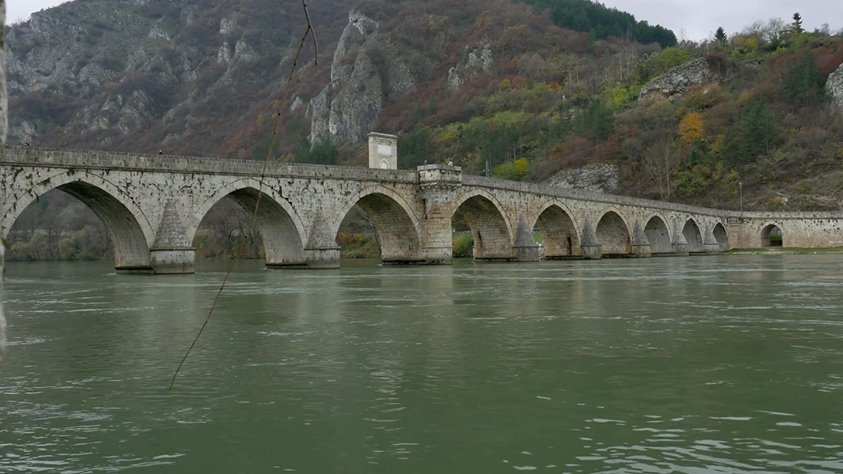
\includegraphics[scale=.25]{images/drina}
\label{drina}
\caption{   }
\end{figure}
1961 ലെ സാഹിത്യത്തിനുള്ള നോബൽ സമ്മാനം ലഭിച്ചത് യുഗോസ്ലാവ്യൻ എഴുത്തുകാരനായ ഇവോ അന് ഡ്രെക്കിനാണ്. (യൂഗോസ്ലാവ്യ എന്ന രാജ്യം ഇപ്പോഴില്ല. തമ്മിൽത്തല്ലി മൂന്ന് രാജ്യങ്ങളായി പിരിഞ്ഞു). ഇവോ അന് ഡ്രെക്കിന്റെ ഏറ്റവും പ്രശസ്തമായ കൃതിയാണ് The bridge on the Drina”. പതിനാറാം നൂറ്റാണ്ടിൽ ബോസ്നിയായിലെ വി ഷെ ഗ്രാഡ് നഗരത്തിൽ തുർക്കികൾ പണിത പാലമാണ് കഥയിലെ നായകൻ. ഫിക്ഷനും ചരിത്രവും ഐതിഹ്യങ്ങളും ഇടകലർത്തിയെഴുതിയിരിക്കുന്ന ഈ മനോഹര പുസ്തകം സാഹിത്യത്തിൽ കമ്പമുള്ളവർ തീർച്ചയായും വായിച്ചിരിക്കണം‌

ബാൾക്കൻ രാജ്യങ്ങളിൽ മിക്കതും പന്ത്രണ്ടാം നൂറ്റാണ്ട് മുതൽ ഇരുപതാം നൂറ്റാണ്ടിന്റെ തുടക്കം വരെ തുർക്കികളുടെ അധീനതയിലായിരുന്നു. തുർക്കിയിലെ ഒട്ടോമൻ സുൽത്താന്റെ അംഗരക്ഷകരായി നിയമിച്ചിരുന്നത് ബോസ്നിയ കാരായ ക്രിസ്ത്യൻ യുവാക്കളെ ആയിരുന്നു. സുൽത്താന്റെ പട്ടാളം ഇടയ്ക്കിടെ വന്ന് പത്തിനും15 നും ഇടയ്ക്കുള്ള ആൺ കുട്ടികളെ ബലമായി ഇസ്താംബൂളിലേക്ക് പിടിച്ചുകൊണ്ടുപോകും അവിടെ വച്ച് അവരെ മതം മാറ്റി സുൽത്താന്റെ സ്വകാര്യ അംഗരക്ഷകസേനയിൽ ചേർക്കും
പതിനാറാം നൂറ്റാണ്ടിന്റെ തുടക്കത്തിൽ ബോസ്നിയയിലെ ഒരു ഗ്രാമത്തിൽനിന്ന് പട്ടാളക്കാർ ഒരു കുട്ടിയെ തട്ടിക്കൊണ്ടുപോയി കുട്ടിയുടെ അമ്മ പട്ടാള സംഘത്തേ കുറേ പിന്തു ടർന്നു.
ബോസ്നിയയുടെയും സെർബിയയുടെയും അതിർത്തിയിലൂടെ ഒഴുകുന്ന ഡ്രിനനദിക്കര വരെ ആ അമ്മ പട്ടാളക്കാരോട് മകനു വേണ്ടി കെഞ്ചി. ഡ്രീനനദി കടക്കാൻ അക്കാലത്തുള്ളത് വഞ്ചി മാത്രം. കടത്ത്കടന്ന് ഇസ്താംബൂളിലേക്ക് പോകാൻ അമ്മയ്ക്ക് സാധിച്ചില്ല.

ഈസ്താംബൂളിലെത്തിയ കുട്ടി പതിവുപോലെ മതം മാറി സുൽത്താന്റെ അംഗരക്ഷക സേനയിൽ ചേർന്നു. കുട്ടി വളർന്നു വലുതായി സുൽത്താന്റെ ഭരണയന്ത്രത്തിന്റെ പ്രധാനിയായി. ഗ്രാൻഡ് വിസിർ അത് അഥവാ പ്രധാനമന്ത്രി പദത്തിൽ വരെ എത്തി.
ഇദ്ദേഹത്തിന്റെ പേര് മുഹമ്മദ് പാഷാ സൊകോളാവിക് എന്നാണ്. പ്രധാനമന്ത്രി പദത്തിൽ ഇദ്ദേഹം 15 വർഷത്തോളം സേവനമനുഷ്ഠിച്ചു മുഹമ്മദ് പാഷാ ഇക്കലത്ത് ഡ്രീന നദിയിൽ ഒരു പാലം പണികഴിപ്പിച്ചു. ഏകദേശം 7 വർഷമെടുത്തു പണിതിരാൻ. നോവലിന്റെ തുടക്കം ഈ പാലത്തിന്റെ ചരിത്രത്തിൽ നിന്നാണ്.

മുഹമ്മദ് പാഷ അധികം കാലം കഴിയുന്നതിനു മുൻപ് എതിരാളികളുടെ കുത്തേറ്റു മരിച്ചു ഇദ്ദേഹത്തിന്റെ മറ്റ് നിർമ്മിതികളെല്ലാം എവിടെയോ പോയ്മറഞ്ഞു. പക്ഷെ ഡ്രീനയിലെ പാലം മാത്രം കാലത്തെ അതിജീവിച്ചു. വി ഷേഗ്രാഡിലെ ഓരാ മനുഷ്യന്റെ ജീവിതത്തിലും പാലം നിർണ്ണായക ശക്തിയായി. ഭരണാധിപന്മാരും പട്ടാളവും രോഗങ്ങളും മാറി മാറി വന്നു ജനങ്ങളാകട്ടെ കലഹിച്ചും സ്നേഹിച്ചും പരസ്പരം കൊന്നൊടുക്കിയും കാലം കഴിച്ചുകൂട്ടി.
വർഷങ്ങൾ കടന്നുപോയി. പാലം എല്ലാറ്റിനും സാക്ഷിയായി. ഒന്നാം ലോകമഹായുദ്ധത്തിൽ സെർബിയൻ വിപ്ളവകാരികൾ പാലത്തിന്റെ ഒരു ഭാഗം തകർക്കുന്നതു വരെയാണ് അന്ഡ്രെക്കിന്റെ നോവൽ

Pട: പാലംത്തിന്റെ ചരിത്രം വീണ്ടും തുടരുന്നുണ്ട്. രണ്ടാം ലോകമഹായുദ്ധത്തിൽ വീണ്ടും പാലത്തിന് കേടുപറ്റി. അയിരത്തിത്തൊള്ളായിരത്തി അൻപതുകളിൽ പാലം നന്നാക്കി. 1992 ൽ നൂറുകണക്കിന് ബോസ്നിയൻ മുസ്ലീങ്ങളെ പാലത്തിൽ വെച്ച് സെർബിയൻ സൈന്യം കൊന്നൊടുക്കി.
2007 ൽ യുനസ്കോ പാലത്തെ ലോക പൈതൃകത്തിന്റെ ഭാഗമായി പ്രഖ്യാപിച്ചു.

കമന്റായി ഒരു ലിങ്ക് ഉണ്ട്. ഇതിൽ നോവലിന്റെ തുടക്കം പാലത്തിന്റെ പടങ്ങൾ വെച്ച് ചിത്രികരിച്ചിരിക്കുന്നു. (Audio book). കാണാൻ മറക്കണ്ട.


  \section{രണ്ടാമത്തെ വായന }
  
   \begin{figure}[H]
  \center
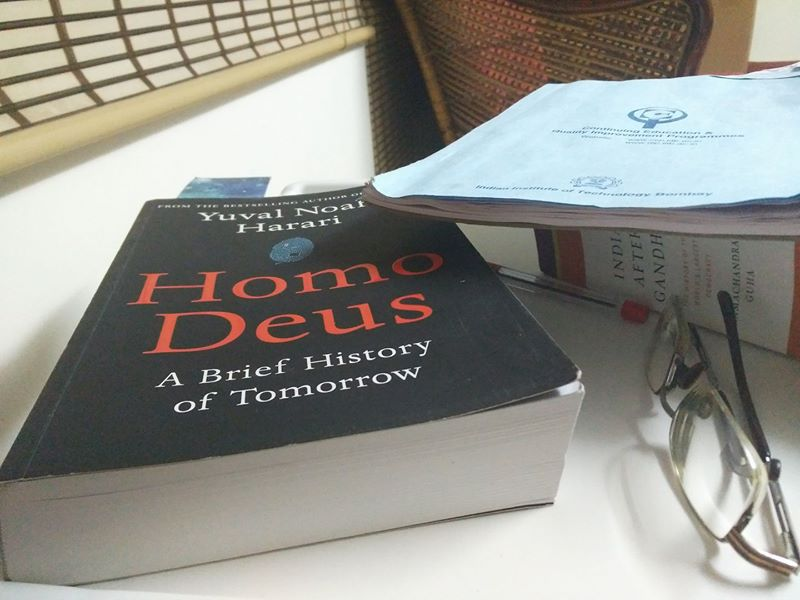
\includegraphics[scale=.25]{images/harari}
\label{harari}
\caption{   }
\end{figure}
  ഇഷ്ടപ്പെട്ട പുസ്തകങ്ങള്‍ രണ്ടാമതും വായിക്കുന്ന ശീലമുണ്ട്. ഈ രണ്ടാമത്തെ വായന പലപ്പോഴും പുതിയ വാതായനങ്ങള്‍ തുറന്ന് തരും. ആദ്യ വായന മിക്കവാറും പെട്ടെന്ന് പുസ്തകാവസാനത്തിലേക്കെത്താനുള്ള ഒരു ഓട്ടമായിരിക്കും. രണ്ടാമത്തേത് നല്ല സമയമെടുത്ത്, ആശയങ്ങളെക്കുറിച്ചൊക്കെ ആലോചിച്ച്, അല്‍പസ്വല്‍പം ബാക്ക്ഗ്രൌണ്ട് റിസേര്‍ച്ച് ഒക്കെ നടത്തിയാണ് പൂര്‍ത്തിയാക്കാറ്. 
  
  കഴിഞ്ഞ മൂന്നുനാലാഴ്ചയായി യൂവാല്‍ ഹരാരിയുടെ Homo Deus രണ്ടാമതും വായിക്കുകയാണ്. ഓരോ പേജുകഴിയുമ്പോഴും വ്യക്തതക്ക് വേണ്ടി കൂടുതല്‍ വായനയും റഫറന്‍സും വേണ്ടി വരുന്നു.. ഈ പുസ്തകത്തിലെ പുൽത്തകിടി കളുടെ സംക്ഷിപ്ത ചരിത്രം എന്ന ഒരു അദ്ധ്യായമാണ് ഇന്ന് വായിച്ചത്. നമ്മള്‍ എന്തിനാണ് ചരിത്രം പഠിക്കേണ്ടതെന്ന്, പുല്‍ത്തകിടികളുടെ (lawn) ചരിത്രം ഉപയോഗിച്ച് ഹരാരി വ്യക്തമാക്കിത്തരുന്നു.
  
   ഹരാരിയുടെ വാദം ഏകദേശം ഇങ്ങനെയാണ്. വീടുപണിയുന്ന ഏതൊരു മധ്യവര്‍ഗ്ഗകുടുംബവും വീടിനുമുന്നില്‍ ചെറിയൊരു പച്ചപുല്‍ത്തകിടി വേണമെന്നാഗ്രഹിക്കുന്നവരാണ്. ഇതുകൊണ്ട് എന്താഗുണം എന്നുചോദിച്ചാൽ കാണാൻ ഭംഗിയുണ്ട് എന്നാവും ഉത്തരം.പുല്‍ത്തകിടികള്‍ മനുഷ്യന്‍ അതിപുരാതനകാലത്തൊന്നും നട്ടുപിടിപ്പിച്ച് തുടങ്ങിയതല്ല. ഗ്രീസിലെ അക്രോപോളിസിലോ റോമിലെ ക്യാപിട്ടോലിയത്തിലോ പുൽത്തകിടി യുണ്ടായിരുന്നതായി ചരിത്ര പുസ്തകങ്ങളിലില്ല.. പ്രത്യേകിച്ചു പ്രയോജന മൊന്നുമില്ലാത്ത പുൽത്തകിടി മനുഷ്യ ഭാവനങ്ങളിൽ ചേക്കേറുന്നത് വളരെ അടുത്ത കാലത്താണ്. മധ്യകാലഘട്ടത്തിലെ യൂറോപ്യന്‍ രാജാക്കന്‍മാരുടേയും പ്രഭുക്കളുടെയും ധനശേഷി പ്രകടിപ്പിക്കുന്നതിനള്ള മാര്‍ഗ്ഗമായിട്ടാണ് പുല്‍ത്തകിടികള്‍ വെച്ചുപിടിപ്പിച്ചു തുടങ്ങിയത്. യൂറോപ്പിലെ വ്യവസായ വിപ്ലവത്തിന്റെ സമയത്ത് മധ്യവര്‍ഗ്ഗഭവനങ്ങളില്‍ കൂടി പുല്‍ത്തകിടി പ്രത്യക്ഷപ്പെട്ടു തുടങ്ങി. രാജക്കാന്‍മാര്‍ ജനാധിപത്യത്തിനും ഏകാധിപതികള്‍ക്കും വഴിമാറിയെങ്കിലും പുല്‍ത്തകിടി പഴയതുപോലെ സ്റ്റാറ്റസ് സിംബലായി നിലനില്‍ക്കുന്നു. 
   
   ഇക്കാലത്ത് പാർലമെന്റുകൾ കോടതികൾ അധികാരികളുടെ ഭാവനങ്ങൾ എന്നിവർ പുല്തത്തകിടിക്ക് നടുക്ക് പരിലസിക്കുന്നു. യൂറോപ്പില്‍ നിന്ന് പുല്‍ത്തകിടികള്‍ കടല്‍ കടന്ന് ലോകം മുഴുവന്‍ വ്യാപിച്ചു . അതിനോടനുബന്ധിച്ച് വിവിധ കച്ചവടങ്ങളും ചെറുകിട വ്യവസായങ്ങളും പുഷ്ടിപ്പെട്ടിട്ടുമുണ്ട്. പുല്‍ത്തകിടികൾ പലയിടത്തും രാഷ്ടിയ അധികാരത്തിന്റെയോ സാമ്പത്തിക മേല്കോയ്മയുടെയോ ചിഹ്നം കൂടിയാണ്. പുല്ലിൽ ചവിട്ടരുത് പോലെയുള്ള ഉഗ്രശാസനകൾ ഈ അധികാരത്തിന്റെ ബഹിർസ്ഫുരണമാണ്. നാം ഒരു പുതിയ വീട്ടിൽ പുല്‍ത്തകിടി വെക്കുമ്പോള്‍ യൂറോപ്യന്‍ പ്രഭുത്വം നമുക്കുമേല്‍ അടിച്ചേല്‍പിച്ച കള്‍ച്ചറല്‍ബാഗേജ് നാമറിയാതെ ചുമക്കുകയാണ്. ചരിത്ര മറിഞ്ഞാല്‍ നമുക്ക് ഇത്തരം സംസ്കാരിക ചുമടുകളിറക്കി വെച്ച്,
   
    നമുക്ക് ലഭ്യമായ, ലഭ്യമാകാമായിരുന്ന മറ്റു സാധ്യതകളേക്കുറിച്ച് ചിന്തിക്കാന്‍ കഴിയുമെന്ന് ഹരാരി പറയുന്നു. ആലോചിച്ചു നോക്കിയാല്‍ പരമ്പാരാഗതമായി നമ്മള്‍ ചെയ്തുകൂട്ടുന്ന ഓരോ കാര്യത്തിനും ഇതുപോലെ ഒരു കള്‍ചറല്‍ ബാഗേജ് കാണും.. അതുകൊണ്ടു തന്നെ ചരിത്ര പഠനം നമ്മുടെ ജീവിത രീതികളുടെയും സംസ്കാരത്തിന്റെയും പുനർ വായനക്ക് സഹായിക്കും. രണ്ടാമത്തെ വായന പോലെ സമയമെടുത്ത് ചെയ്യേണ്ട ഒന്നാണ് ചരിത്ര പഠനവും.   
    
\section{The Raqqa Diaries}
\begin{figure}[H]
  \center
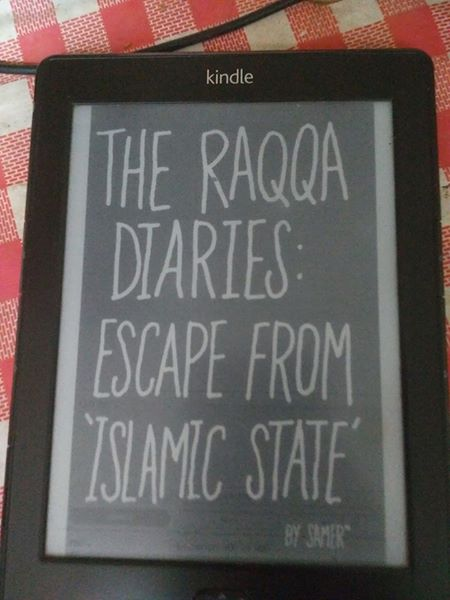
\includegraphics[scale=.25]{images/raqa}
\label{raqa}
\caption{   }
\end{figure}
യൂഫ്രട്ടീസ് നദി തീരത്തുള്ള ഒരു സിറിയൻ പട്ടണമാണ് റാഖ. പുരാതന സംസ്കാരങ്ങളുടെ കളിത്തൊട്ടിലായിരുന്നു ഇവിടം. കഴിഞ്ഞ കുറേ വർഷങ്ങളായി സിറിയയിൽ ആഭ്യന്തര യുദ്ധം നടക്കുകയാണ്. ആരൊക്കെ ആ ആർക്കൊക്കെ എതിരെയാണ് യുദ്ധത്തിലേർപ്പെട്ടിരിക്കുന്നതെന്ന് മനസ്സിലാക്കണമെങ്കിൽ ഈ പ്രദേശത്തിന്റെ ചരിത്രം വിശദമായി പഠിക്കേണ്ടി വരും. സിറിയയിൽ പ്രസിഡന്റ് ആസദിന്റെ കുടുബംഭരണമാണ്. ഇദ്ദേഹത്തിന്റെ സൈന്യം, കുർദുകൾക്ക് മുൻതുക്കമുള്ള SDF, ഐസിസ് എന്നിവർ ഇപ്പോഴും പോരാടുകയാണ് റാഖയിൽ. 2013 ൽ ഇസ്ലാമിക് സ്റ്റേറ്റ് റാഖ പിടിച്ചെടുത്ത് അവരുടെ തലസ്ഥാനമാക്കി. ഐ എസിന്റെ ആശയങ്ങൾ നടപ്പാക്കുന്നതിന്റെ ഭാഗമായി ജനതയുടെ മേൽ അതിക്രൂരമായ നിയമങ്ങൾ അടിച്ചേൽപ്പിക്കപ്പെട്ടു. ഇസ്ലാമിക് സ്റ്റേറ്റിന്റെയും അസദ് ഭരണകൂടത്തിന്റെയും മറ്റ് വിദേശ ശക്തികളുടെയും ഇടയിൽപ്പെട്ടു പോയ ഒരു ജനത്തിന്റെ കഥയാണ് The Raqqa Diaries Escape from Islamic state എന്ന ചെറു പുസ്തകം. . 24 കാരനായ ഗ്രന്ഥകാരൻസമീർ എന്ന തൂലികാനാമത്തിലാണുള്ളത്. ഇയാൾ ഐ എസിന്റെ ഇസ്ലാമിക വിപ്ലവം തുടങ്ങിയ കാലത്ത് ഒരു സർവ്വകലാശാല വിദ്യാർത്ഥിയായിരുന്നു. അക്കാലം മുതൽ 2016ൽ റാഖാ യിൽ നിന്ന് രക്ഷപെടുന്നതു വരെ നഗരത്തിൽ സംഭവിച്ച കാര്യങ്ങളുടെ ഭീതിപ്പെടുത്തുന്ന വിവരണമാണീ കുറിപ്പുകൾ. 
  


\section{ചെമ്പൻമുടിക്കാരി }    
    പാമുക്കിന്റെ ചെമ്പൻമുടിക്കാരി ഒറ്റയിരുപ്പിന് വായിച്ചു കഴിഞ്ഞു. മിത്തും ഫിലോസഫിയും മേമ്പൊടി ചേർത്ത് എഴുതിയ മിസ്റ്ററി . ഫിർദൗസിയുടെ Shahnameh യിലെ സൊഹറാബിന്റെയും റസ്തത്തിന്റെ കഥയുടേയുംഗ്രീക്ക് മിത്തോളജി യിലെ ഇഡിപ്പസ് രാജാവിന്റെ കഥയുടേയും പശ്ചാത്തലത്തിലാണ് നോവൽ വികസിക്കുന്നത്. ആദ്യഭാഗം 1980 കളിൽ സെമം എന്നൊരാളുടെ ജീവിതാനുഭവങ്ങളിൽ നിന്നാണ് തുടങ്ങുന്നത്. അക്കാലത്തയാൾ മെഹമൂത് എന്നൊരു കിണർ പണിക്കാരന്റെ സഹായിയായി കഴിയുമ്പോളാണ് അവിചാരിതമായി ചെമ്പൻമുടിക്കാരിയെ കണ്ടെത്തുന്നത്. അവർ സന്ധിക്കുന്നതാകട്ടെ ഒരു രാത്രി മാത്രം. ചെമ്പൻമുടിക്കാരി സെമിന്റെ പിതാവിന്റെ പൂർവ്വ കാമുകിയാണെന്ന കാര്യം അയാൾ അറിയുന്നുമില്ല. രണ്ടാം ഭാഗത്ത് സെം പണക്കാരനായ ഒരു ബിൽഡിംഗ് കോൺട്രാക്ടറാണ്. ഒരു നാൾ എൻവർ എന്നൊരാൾ സെമ്മിന് ചെമ്പൻമുടിക്കാരിയിലുണ്ടായ മകനാണെന്ന് അവകാശപ്പെടുന്നു. കോടതി DNA പരിശോധിച്ച് പിതൃത്വം തെളിയിക്കുന്നു. തുടർന്ന് അച്ഛനും മകനും കണ്ടുമുട്ടുന്നു. സസ്പെൻസ് കളയുന്നില്ല. പാമുക്കിന്റെ ഈ മനോഹര രചന ഫിക്ഷനിൽ താൽപര്യമുള്ളവർക്ക് റക്കമെന്റ് ചെയ്യുന്നു.
    
    \begin{figure}[H]
  \center
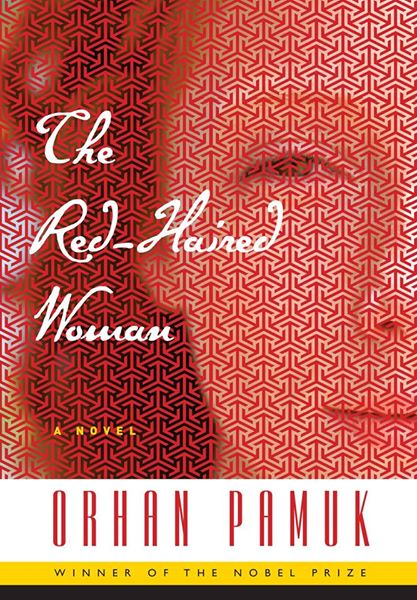
\includegraphics[scale=.25]{images/pamuk}
\label{pamuk}
\caption{   }
\end{figure}

    \section{കോട്ടയം പുഷ്പനാഥ്  }
    ഞാൻ വായന തുടങ്ങിയ കാലം മുതൽ കോട്ടയം പുഷംനാഥിന്റെ ആരാധകനാണ്. ലൈബ്രറി കളിൽ തേടിനടന്ന് പുഷ്പനാഥിനെ വായിച്ചിട്ടുണ്ട്. പുസ്തകങ്ങൾക്ക് catching ആയ പേരുകളിടുന്നതിൽ പുഷ്പനാഥിനെ വെല്ലാൻ മലയാളത്തിലാരുമില്ല. നി .കൊ. ഞ ച എന്നും ഇമ യൗ എന്നും സിനിമക്ക് പേരിടുന്നവർ കോട്ടയം പുഷ്പനാഥിനെ കണ്ടുപഠിക്കണം എന്തെല്ലാം കിടിലൻ പേരുകളാണ്. തൈമൂറിന്റെ തലയോട് , ഡ്രാക്കുള കോട്ടയിൽ സുന്ദരികൾ, നാലാം വളവിലെ നാഗ യക്ഷി, ഫറവോന്റെ മരണ മുറി. ഡ്രാക്കുളയുടെ അങ്കി. പേരു കണ്ടാൽ വാങ്ങി വായിച്ചു പോകും. 
    
 
\begin{figure}[H]
  \center
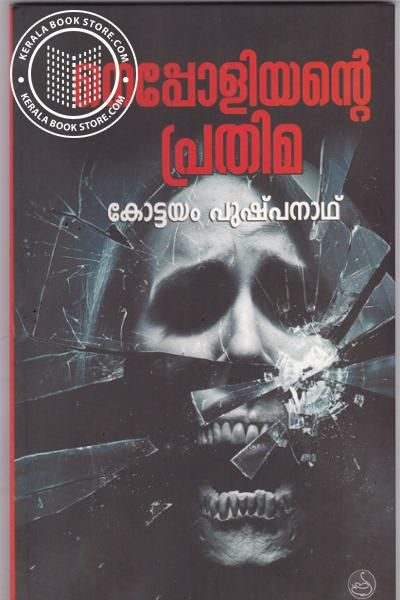
\includegraphics[scale=.25]{images/push}
\label{push}
\caption{   }
\end{figure}    
    
    ഫറവോന്റെ മരണ മുറിയായിരുന്നു ഒരു കാലത്ത് എന്റെ ഇഷ്ട പുസ്തകം. ഫറവോന്റ മരണ മുറിയിൽ നിന്ന് ഒരു ഭാഗം . " പേടിപ്പെടുത്തുന്ന ആ അന്തരീക്ഷത്തില്‍ അവള്‍ തന്നെത്തന്നെ സൂക്ഷിച്ചുനോക്കിക്കൊണ്ടിരിക്കയാണ്‌. അവള്‍ എന്താണ്‌ അനങ്ങാത്തത്‌? ഇമകള്‍ വെട്ടിക്കാത്തത്‌? സര്‍വ്വധൈര്യവും കേന്ദ്രീകരിച്ചുകൊണ്ട്‌ മാര്‍ക്സിന്‍ അവളുടെ നേര്‍ക്കടുത്തു. അടുത്തു ചെന്നു. അപ്പോഴും അവള്‍ കണ്ണിമയ്‌ക്കാതെ മാര്‍ക്സിന്‍ അല്‍പ്പനിമിഷം നിന്നു. എന്തും വരട്ടെയെന്നു കരുതി കസേരയുടെ കയ്യില്‍ അമര്‍ന്നിരുന്ന അവളുടെ കൈത്തണ്ട ഉയര്‍ത്തി. അത്‌ തണുത്ത്‌ വിറങ്ങലിച്ചിരുന്നു.. കൈ അയച്ചപ്പോള്‍ ഒരു മരണംപോലെ അവ വീണ്ടും അതേ സ്ഥാനത്തു പതിച്ചു. " പുഴ ബുക്സിൽ പുഷ്പനാഥിന്റെ പുസ്തകങ്ങളുണ്ട്. എല്ലാം കൂടെ വാങ്ങി ഒന്നു കൂടെ വായിച്ചാലോ. http://www.puzha.com/malayalam/bookstore/cgi-bin/author-detail.cgi?code=542 
    
    മനോരമയിൽ വന്ന പുഷ്പനാഥിന്റെ ഇന്റർവ്യു. https://youtu.be/2YX-6uaz9q8
    
\section{ പകുതി വഴി നിന്നുപോയവ }
        \section{Introducing classics to children}
        \section{Why engineer should read literature?}
\chapter{Troll}

\section{സ്വാതിനഗർ}
നുമ്മ ഗഡി Jayant Mammen ഉളമ്പാറയേക്കുറിച്ച് മാേഹൽ ലാൽ നായകനായ കഥയെഴുതുന്നുന്ന്. എങ്കി ഈ കഥ കൂടകിടക്കട്ടെ. ഒരു ഊളമ്പാറക്കഥ. 

" വിട് എവിടെയാ "

 "തിരുവനന്തപുരം " 
 
 "തിരുവനന്തപുരത്ത് ?"
 
  "പേരൂർക്കട " 
  
  "അവിടെ "
  
   " സ്വാതിനഗർ " 
   
   " സ്വാതി നഗറോ?അതെവിടെ " 
   
   "പേരുർക്കട നിന്ന് ശാസ്തമംഗലം വഴിയിൽ ഒരു കിലോമീറ്റർ. ഹിന്ദുസ്ഥാൻ ലാറ്റക്സിനടുത്ത് "
   
    "ഓ! നമ്മടെ ഊളൻപാറ " 
    
    " എയ് അല്ല സ്വാതി നഗർ "
\section{നസ്രാണി ഉണരുമ്പോൾ}

 കഴിഞ്ഞ അമ്പതു വർഷമായി എന്റെ ഉള്ളിലെ നസ്രാണി ഉണരാൻ ശ്രമിക്കുകയാണ് .ശശികല ടീച്ചറുടെ ജല്പനങ്ങളും വട്ടായിലച്ചന്റെ വചന പ്രബോധനവും പലകുറി കേട്ടിട്ടും വാറ്റുചാരായം കൊണ്ടാത്മാഭിഷേകം നിരവധി തവണ നടത്തിയിട്ടും അവനുണരുന്നില്ല. ആത്മജ്ഞാനത്തിന്റെ ആന്തുറിയം തേടി എൻറെ ആത്മാവ് കേരളത്തിലങ്ങോളമിങ്ങോളം അലയുകയാണ്. എപ്പോഴെങ്കിലും ഉള്ളിന്റെ ഉള്ളിൽ നിന്നും ആ നസ്രാണി ഉണർന്ന് പുറത്തു വരാതിരിക്കില്ലെന്ന പ്രതീക്ഷ ഇപ്പോഴുമുണ്ട്. ഇടവകയിൽ നിന്ന് ഇടവക തോറും കല്യാണവും മാമോദിസയും പെരവാസ്തോലിയുമുണ്ട് ഞാൻ അങ്ങനെ നടക്കും, അവനെ ഉണർത്താൻ വേണ്ട കുണ്ഡലനിയെ തേടി. പൂർവികർ പലർക്കും ഇതിനു വേണ്ട മന്ത്രം അറിയാമായിരുന്നു. പക്ഷെ ആരും പറഞ്ഞു തന്നില്ല. സ്വയം കണ്ടെത്തണമത്രെ.
   \begin{figure}[H]
  \center
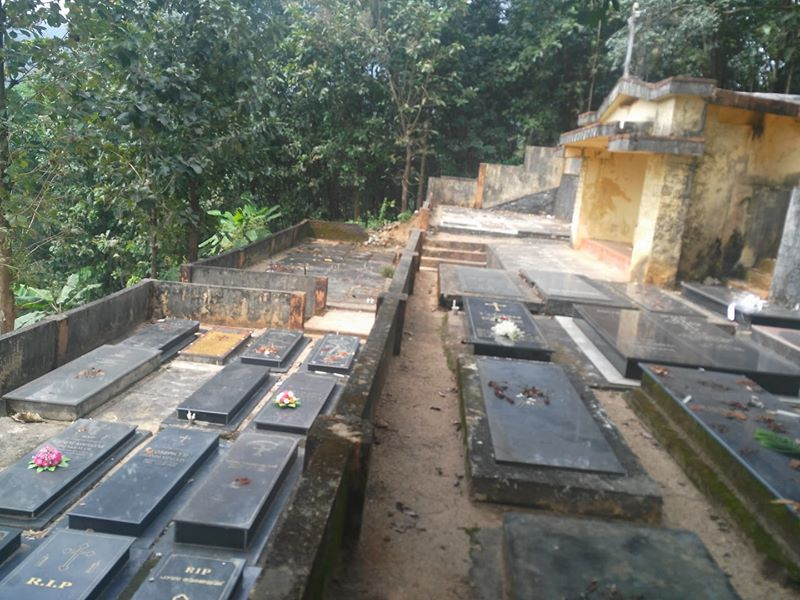
\includegraphics[scale=.25]{images/nas1}
\label{nas1}
\caption{   }
\end{figure}
  ഈയിടെയായി മലമുകളിലൂടെ യാത്ര ചെയ്യുമ്പോൾ ആത്മാവിന് ഒരു ഉണർവ്വ് തോന്നുന്നുണ്ട്. ഇപ്പോൾ എനിക്കറിയാം ഞാൻ തേടുന്ന ആ മന്ന മലഞ്ചെരുവിലെവിടെയോ മറിഞ്ഞിരിക്കുന്നു. ഓരോ യാത്രയും അതു തേടിയാണെന്നും. ഇന്ന് കാഞ്ഞിരപ്പുഴ പാലക്കയം പള്ളിയുടെ സെമിത്തേരിയിലുറങ്ങുന്ന കാരണവൻമാരോട് ആദിവ്യ മാർഗം ചോദിച്ച് കുറേ നേരം നിന്നു. ആകെ മൂകത ആരും മിണ്ടുന്നില്ല. പെട്ടെന്ന് ആത്മാവിന്റെ അന്തരാളത്തിൽ നിന്നും ഒരു നവ മുകുളം പൊട്ടിമുളയ്ക്കുന്ന മൃദു സ്വരം കേട്ട് മാതിരി. എനിക്ക് സംശയമായി ഇനി അവനെങ്ങാനും ഉണർന്നോ ? ഞാൻ ചിന്തിച്ചുനോക്കി. എന്താവും കാര്യം ? ചുറ്റും സസൂക്ഷ്മം വീക്ഷിച്ചു. അപ്പോഴാണ് കാര്യം പിടികിട്ടിയത് ഞാൻ നിൽക്കുന്നത് അധ്വാനവർഗ്ഗ സിദ്ധാന്തത്തിൻറെ പ്രായോജകരും പ്രയോക്താക്കളുമായ ഒന്നു രണ്ടു തലമുറകൾ കൃഷിചെയ്ത മലമുകളിലാണ്. ഇവിടെ ആകെ ഒരു സംഗീതമേ യുള്ളു. കാരിരുമ്പ് കത്തി കൊണ്ട് സ്വന്തം ശരീരം ആസകലം വരഞ്ഞു കീറി തലമുറകൾക്ക് പാൽ ചുരത്തി നിൽക്കുന്ന റബർ മരങ്ങളുടെ താളാത്മകമായ തലയാട്ടിലിന്റെ മൃദു സ്വരം. അവന്റെ പാൽ കുടത്തിലേക്ക് നോക്കിയപ്പോഴാണ് പ്പോഴാണ് എന്റെ ഉള്ളിലെ നസ്രാണി ഉണരാൻ നോക്കിയത്. തലമുറകളുടെ കണ്ണീരാണവൻ ചുരത്തിയിട്ടിരിക്കുന്നത്. ഇതു കണ്ടാൽ ഉറക്കം നടിക്കുന്നവൻ വരെ ഉണരും.
     \begin{figure}[H]
  \center
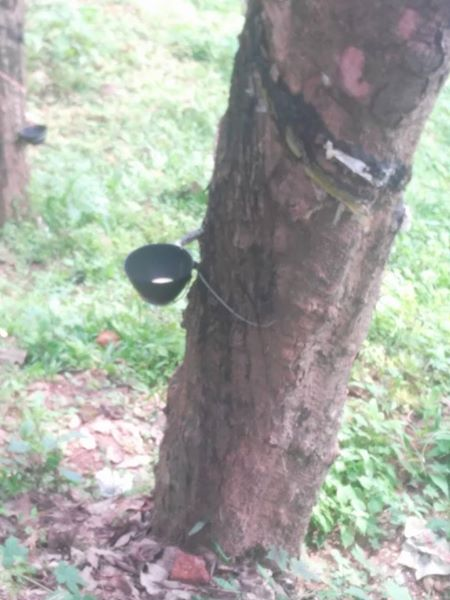
\includegraphics[scale=.25]{images/nas2}
\label{nas2}
\caption{   }
\end{figure}
\section{ഷാപ്പ് പള്ളിയും പള്ളി ഷാപ്പും.}
  കോട്ടയത്തെ ഒരുൾനാടൻ പ്രദേശത്താണ് കഥാനായകനായ ഷാപ്പുള്ളത്. അക്കാലത്ത് ഇവിടേക്ക് ആകെ ഒരു ബസേ യുള്ളു. ഷാപ്പിനു മുമ്പിൽ വണ്ടിക്ക് സ്റ്റോപ്പുണ്ട്. സ്വാഭാവികമായും സ്റ്റോപ്പിന്റെ പേര് ഷാപ്പും പടി എന്നായി. ഇങ്ങനെയിരിക്കെ ഷാപ്പി നോട് ചേർന്ന പുരയിടം പള്ളിക്കാർ വാങ്ങി. പുതിയതായി വന്ന വികാരി നാടുനീളെ പിരിവെടുത്ത് സുന്ദരൻ പള്ളി ഒരെണ്ണം പണിതു. പണി കഴിഞ്ഞതോടെ അച്ചനെ അടുത്ത പണിസ്ഥലത്തേക്ക് മാറ്റി. പള്ളിയും ഷാപ്പും സഹവർത്തിത്വത്തിൽ അങ്ങനെ കഴിഞ്ഞു കൂടി. 
   \begin{figure}[H]
  \center
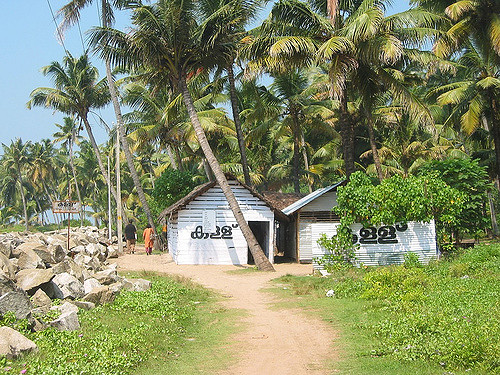
\includegraphics[scale=.45]{images/shapu}
\label{shapu}
\caption{   }
\end{figure}
  
  ചില പിന്തിരിപ്പൻമാർ ഷാപ്പുപള്ളി ന്ന് പേരിട്ടെങ്കിലും അത് കർത്താവും വിശ്വാസികളും മൈന്റ് ചെയ്തില്ല. കർത്താവ് വൈകിട്ടാകുമ്പം കുരിശേന്നിറങ്ങി ഒരു കുപ്പി അന്തി അടിക്കും. സഹ കൂടിയൻമാരുടെ കൂടെ "എന്തതിശയമെ "പാടും . മൂന്നാല് കൊല്ലം കഴിഞ്ഞപ്പോൾ വികാരി വീണ്ടും മാറി. ഇത്തവണ വന്നത് ഒരു പ്രാർത്ഥനാ വിദഗ്ദനായിരുന്നു. പ്രത്യേകിച്ച് ഡ്യൂട്ടി യൊന്നുമില്ലാതെ റോമിൽ കൂടെ അലഞ്ഞ് തിരിഞ്ഞിരുന്ന ഒരു പുണ്യാളനെ പൊക്കിയെടുത്ത് ബുധനാഴ്ച നൊവേന തുടങ്ങി. പുണ്യാളൻ കല്യാണം നടത്തിക്കൊടുക്കുന്നതിൽ സ്പെഷലൈസ് ചെയ്തിരുന്നതുകൊണ്ട് ഷാപ്പുപള്ളിയുടെ പേര് കൂടിക്കൂടി വന്നു.
  
   പതിയെ ബസിന്റെ ബോർഡിലൊക്കെ ഷാപ്പുപള്ളി വഴി എന്ന് ബോർഡ് വന്നു. ബുധനാഴ്ച ഷാപ്പിലും തിരക്കായി. കറിയൊക്കെ ഫേമസാകാൻ തുടങ്ങി. മുന്ന് നാല് കൊല്ലം കഴി ഞ്ഞ് ഷാപ്പുപള്ളി ഇടവകക്കാർ കർത്താവിന് ബസേന്നിറങ്ങി വിശ്രമിക്കാനുള്ള ഒരു കുരിശുപള്ളി പണിതു. കമ്മറ്റി കൂടി കുരിശുപള്ളി വെഞ്ചിരിപ്പിനായി ബിഷപ്പിനെ വരുത്താൻ തീരുമാനിച്ചു. ബിഷപ്പുമാർ പൊതുവെ മദ്യവിരുദ്ധരാണല്ലോ. നമ്മുടെ ബിഷപ്പിനും ഷാപ്പ് തീരെ പിടിച്ചില്ല, ബസ്റ്റോപ്പിന്റെ പേരും. കുരിശുപള്ളി വെഞ്ചിരിച്ചോണ്ടിരുന്നപ്പം കടന്നു പോയ ബസിൽ ഷാപ്പു പള്ളി വഴി എന്ന് എഴുതിട്ടുള്ളതും മൂപ്പർ കണ്ടു. ആകെ കലിപ്പായി. വിശ്വാസികൾ ഇളകി മറിഞ്ഞു. താമസിയാതെ മദ്യവിരുദ്ധ സമരം തുടങ്ങി. മെഴുകുതിരി , ഉപവാസ പ്രാർത്ഥന ഇത്യാദി പ്രയോഗങ്ങൾ ഷാപ്പിന് പബ്ലിസിറ്റി കൂട്ടി. സമരം അക്രമാസക്തമായി, കോടതി പോലിസ് ഒക്ക വന്നു. ഷാപ്പിനും പള്ളിക്കും വരുമാനം കൂടി.
   
    അവസാനം മാണി സാറൊക്കെ ഇടപെട്ടു. എന്തിനും ഒരു അവസാനം വേണ്ടെ . ഷാപ്പ് ഒരു കിലോമീറ്റർ അപ്പുറത്തേക്ക് മാറ്റാനും ബസ് സ്റ്റോപ്പിന്റെ പേര് ശാലോം നഗർ എന്നാക്കാനും വിശ്വാസികൾ ആരും പള്ളിയെ ഷാപ്പു പള്ളി എന്ന് വിളിക്കരുതെന്നും എല്ലാ ബസിലും പുതിയ സ്ഥലപ്പേരെഴുതാനും സർവ്വകക്ഷിയോഗം തീരുമാനിച്ചു. കുടിയൻമാർക്കും കർത്താവിനും വഴിതെറ്റാ തിരിക്കാൻ ഷാപ്പ് കോൺട്രാക്ടർ പഴയ ഷാപ്പിന്റെ സ്ഥാനത്ത് പുതിയ ഷാപ്പിലേക്കുള്ള വഴി എഴുതിവെക്കാൻ അനുവാദം വേണമെന്ന് ആവശ്യപ്പെട്ടു. സർവകക്ഷിക്കും സമ്മതം. ഇനിയാണ് ട്വിസ്റ്റ് . പിറ്റേന്ന് പള്ളിയുടെ മുൻപിൽ റോഡരുകിൽ സൈൻബോർഡ് പൊന്തി. പള്ളിഷാപ്പ് ദൂരം ഒരു കി. മി .
    
    % PS: (ഇത് വായിക്കാതെ കമന്റരുത്. ) 1)തള്ളൽ പ്രസ്ഥാനത്തിന് തനത് സംഭാവന നൽകിയിട്ടുള്ള ഒരു സുഹൃത്ത് പണ്ട് പറഞ്ഞ കഥയാണിത്. ഈ കഥ യിൽ എത്രമാത്രം യാഥാർത്യമുണ്ടെന്ന് അറിയില്ല. 80കളിലൊ മറ്റോ ആയിരിക്കണം. 2) പള്ളിയെ പരിഹസിച്ചുന്ന് പറഞ്ഞ് കുരു പൊട്ടുന്നവർ താഴെ ഇട്ടിരിക്കുന്ന കുത്ത് ലൈക് ചെയ്യണം 3) അച്ചായൻമാർക്ക് പണി കിട്ടിയല്ലോ എന്ന് കരുതുന്നവർ (സുഡു സംഘി ടിം)അതിന്റെ താഴെയുള്ള കോമലൈക്കണം. 4) കള്ളുഷാപ്പിന്റെ അനുഭാവികൾക്ക് വേണ്ടി അതിനും താഴെ ഒരു ഐറ്റം കൊടുത്തിട്ടുണ്ട്
\section{പൂജ}
''ഹലോ "

"ഹലോ മാങ്ങാ മാർട്ടിന്റെ കസ്റ്റമർ കെയറിലേക്ക് സ്വാഗതം. ഞാൻ അജിത്. നിങ്ങളുടെ കോൾ റെക്കോഡ് ചെയ്യുന്നതാണ്‌. സർ പറഞ്ഞോളു "

"നിങ്ങളുടെ വെബ്സൈറ്റിൽ കുടി മുപ്പത് മുട്ട ഓഡർ ചെയ്യാൻ നോക്കുകയാണ്. വർക്കാകുന്നില്ല"

"വെബ് സൈറ്റ് പൂജക്ക് വെച്ചിരിക്കുകയാണ് സർ. മുട്ട മറ്റന്നാൾ കിട്ടും"

"ങേ"

''സർ മറ്റെന്തെങ്കിലും "

"എങ്കിൽ താൻ ആ ഫോൺ കൂടെ അങ്ങ് പൂജക്ക് വെക്ക്."

\section{ചക്ക മാഹാത്മ്യം}
 ചക്ക സീസൺ തുടങ്ങുന്നത് ഡിസംബർ അവസാനത്തോടു കൂടിയാണ്. കട്ടിക്കാലത്ത് മിക്കവാറും ക്രിസ്തുമസ് അവധിക്കായിരിക്കും ആ സീസണിലെ ആദ്യ ചക്ക മൂക്കുന്നത്. മീനച്ചിൽ തൊടുപുഴ ബെൽറ്റിൽ ചക്ക പുഴുങ്ങുകയാണ് ചെയ്യുന്നത്.തിരുവനന്തപുരത്തേ പോലെ കറിവെക്കില്ല. (ചക്ക കറി വെക്കുന്നവർ താഴേക്ക് വായിക്കണമെന്നില്ല.:D) പുഴുക്കുതന്നെ രണ്ടു രീതിയിൽ ഉണ്ട്. ചക്ക ഉപ്പേരിപ്പരുവത്തിൽ അരിഞ്ഞ് അൽപം വെള്ളമൊഴിച്ച് വേവിക്കും തേങ്ങ മഞ്ഞൾ കാന്താരി വെളുത്തുള്ളി ഒക്ക അരച്ച് ഇതിലിട്ട് ഇളക്കും. ഇതാണ് സാധാരണ ഉണ്ടാക്കുന്ന പുഴുക്ക്. ഇത് ഇളക്കുമ്പോഴുള്ള മണം tantalizing ആണ്. ഇതിന്റെ കൂടെ കോഴിക്കറി ബെസ്റ്റാണ്. ഇല്ലെങ്കിൽ മുളക് പൊട്ടിച്ചതായാലും മതി. ഈ സിസണിൽ ഇവിടുത്തെ ഷാപ്പിലൊക്കെ കിട്ടും. പനങ്കള്ളിന്റെ കൂടെ അത്യത്തമം. രണ്ടാമത്തേ രീതിക്ക് ചക്ക അരിഞ്ഞു പുഴുങ്ങുക എന്നാണ് വീട്ടിൽ പറഞ്ഞു കേട്ടിട്ടുള്ളത്. നല്ല മൂത്ത ചക്ക നല്ലവണ്ണം വേവിച്ച് ഒരു സെമി ലിക്വിഡ് പരുവമാകും. ഇതിലേക്ക് തേങ്ങ ച്ചമ്മന്തി ഒഴിച്ച് കഴിക്കാൻ നല്ല രസമാണ്. ഇതിൽ മഞ്ഞൾ ചേർക്കില്ല. അതു കൊണ്ട് ചിലർക്കൊക്കെ അത്ര പിടിക്കില്ല. ഈ സിസണിലെ ആദ്യ ചക്കപ്പുഴുക്ക് നാടൻ കോഴിക്കറിക്കൊപ്പം കഴിച്ച് മകിഴ്ചിയടഞ്ഞ നിങ്ങളുടെ സ്വന്തം ലേഖകൻ പൂഞ്ഞാറിൽ നിന്ന്.
 \section{ഡിങ്കോയിസ്റ്റു സിനിമാക്കഥ  }
 മുൻകൂർ ജാമ്യം. എസ്രതിയേറ്ററിൽ പോയി കണ്ട ഒരു ഹതഭാഗ്യൻ എഴുതിയതാണ്. എല്ലവരും ടി വി യിൽ കണ്ട സ്ഥിതിക്ക് വീണ്ടും റിലീസാക്കുന്നു. എന്റെ ഡിങ്കോയിസ്റ്റു സുഹൃത്തുക്കളോട് ഒരു അഭ്യർത്ഥനയുണ്ട്. ഉടനെ തന്നെ നിങ്ങളുടെ കൈവശമുള്ള വി.ബാലമംഗളത്തിന്റെ കോപ്പികൾ ഒരു വിഞ്ഞപ്പെട്ടിയിലിട്ട് വല്ല കക്കൂസ് ടാങ്കിലോ തട്ടിൻപുറത്തോ മറ്റോ ഒളിപ്പിക്കുക. പെട്ടിയുടെ പുറത്ത് ഡിങ്ക ചിഹ്നങ്ങൾ രേഖപ്പെടുത്താൻ മറക്കരുത്. കഴിയുമെങ്കിൽ നഴ്സറി കുട്ടികളുടെ രണ്ട് നോട്ടുബുക്കും ഇട്ടേക്കണം. പട്ടി പൂച്ച ആന എന്നീ മൃഗങ്ങളുടെ ചിത്രങ്ങളുള്ള ബുക്കാണ് വേണ്ടത്. ഭാവിയിലെ മലയാള സിനിമക്ക് വലിയ സംഭാവനയാവും ഇത്. ഡിങ്കോയിസ്റ്റുകൾക്ക് കേരളത്തിൽ അധിക കാലം തമസിക്കാനാവുമെന്ന് ഞാൻ കരുതുന്നില്ല. അല്ലെങ്കിൽത്തന്നെ ഡിങ്കന്റെ കാഹളം കേൾക്കുമ്പോൾ പങ്കിലക്കാട്ടിലേക്ക് പാലായനം ചെയ്യേണ്ടതുണ്ടല്ലോ. ഇനി ഒരു നൂറ് നൂറ്റമ്പത് വർഷം കഴിഞ്ഞുള്ള സിനാറിയോ നോക്കാം. സംവിധായകനാകാൻ നടക്കുന്ന 54 സപ്ലിയുള്ള ഒരു ബിടെക് പയ്യൻ അവിചാരിതമായി കക്കൂസ് ടാങ്ക് തുറക്കുന്നു. ബാലമംഗളവും നേഴ്സറി ബുക്കും കാണുന്നു. ബുക്ക് വായിക്കുമ്പോൾത്തന്നെ പയ്യന് ഇത് പുരാതന ഡിങ്കോയിസ്റ്റ് തന്റെ കാറിന് തൃശ്ശൂർ പൂരത്തിന്റെ സമയത്ത് അള്ളുവെച്ച ഏതോ ഒരുവ നോട് പ്രതികാരം ചെയ്യാനായി ഒരു പൂച്ചയെ ആവാഹിച്ച് ഇരുത്തിയിരിക്കുന്നതാണെന്ന് മനസിലാക്കുന്നു. ബാലമാഗളത്തിലാണെങ്കിൽ ഡിങ്കന്റെ പൂർണ്ണകായ ചിത്രവും. പയ്യന്റെ ഭാവന ചിറക് വിടർത്തുകയാണ് സൂർത്തുക്കളേ. ഇനി തിരക്കഥയെഴുത്തായി. കഥയും കഥാപാത്രങ്ങളും സാങ്കൽപികം. ഏകദേശ രൂപം ഇങ്ങനെയാണ്. (ദേശിയ ഗാനവും ശ്വാസകോശവും ആവശ്യത്തിന് ചേർക്കണം.) ലാലൂരിലെക്ക് വേസ്റ്റ് എടുക്കാൻ കോൺട്രാക്ട് ആയി ഓടുന്ന ലോറിയുടെ കിളിയാണ് നായകൻ. വിഞ്ഞപ്പെട്ടിയിലുള്ളപുച്ചയെ ഉപയോഗിച്ച് തൃശ്ശൂർ പട്ടണത്തെ പൂരത്തിന്റെ ദിവസം നാറ്റിക്കാനാണ് പുരാതന ഡിങ്കോയി്സ്ററിന്റെ പദ്ധതി. പൂച്ചയുടെ പ്രേതം കിളിയിൽ പരകായപ്രവേശം ചെയ്യുന്നത് അവന്റെ ഭാര്യയിലൂടെയാണ്. ആ പാവം സ്ത്രി ആക്രിക്കടയിൽ നിന്ന് കോഴിയെവിരിയിക്കാനായി വിഞ്ഞപ്പെട്ടി വാങ്ങുന്നു. പെട്ടി തുറന്നതും പ്രേതം കട്ടിൽ കീഴിലൊളിക്കുന്നു. തുടർന്ന് പലതവണ നായകനെ വരുതിയിലാക്കാൻ നോക്കുന്നു. ഇവിടെ രാത്രിസീ നൊക്കെ ഇടാം. അവസാനം നായകൻ മാക്ക്ബുക്ക് തുറന്ന് കോൺജുറിംഗ് 2 കാണുമ്പോൾ സ്ക്രിൻബ്ലാങ്കാക്കിയാണ് നായകന്റെയുള്ളിൽ കയറുന്നത്. ഡിങ്കോയിസ്റ്റ് ന്റെ പ്രതികാരം കിളിയിലൂടെയാണ് നടപ്പാക്കാൻ പോകുന്നത്. കിളിയാകുമ്പോ വേസ്റ്റ് ലോറിക്ക് സ്വരാജ് റൗണ്ടിൽ വെച്ച് തന്നെ അള്ളുവെക്കാൻ എളുപ്പമാണ്. ഇത് പൂര ദിവസം നടപ്പാക്കാനാണ് ഉദ്ദേശിക്കുന്നത്. ഇനി പൂച്ച കരയുന്ന കുറെ സീൻ വേണം. കിളിയുടെ ഭാര്യ കുരിശ്, പൂച്ച,കണ്ണാടി ഒക്കെ ആവശ്വത്തിന് ചേർക്കാം. പ്രേത കഥയല്ലെ. ഈ പദ്ധതി സ്വപ്നത്തിൽ മണത്തറിയുന്ന ലോറി ഡ്രൈവർ പരിഭ്രാന്തനാകുന്നു. കിളിയുടെ ഭാര്യയിൽ നിന്ന് ബാലമംഗളത്തിന്റെ ഫോട്ടോ സ്റ്റാറ്റ് എടുത്ത് ബോംബേ ക്ക് അയക്കുന്നു. അധോലോകത്തിന്റെ സഹായത്താൽ ഡിങ്കോയിസ്റ്റുകൾ മൊത്തം പങ്കിലക്കാട്ടിലാണെന്ന് കണ്ടെത്തുന്നു. പങ്കാലക്കാട്ടിൽ നിന്ന് ടൂർ വന്ന ഒരു ലോറി ഡിങ്കോയിസ്റ്റുകളെ കപ്പയും മീൻ കറിയും കൊടുത്ത് വരുത്തുന്നു. ഇക്കുട്ടത്തിൽ ഒരു ഡിങ്ക മത ബിഷപ്പുമുണ്ട്.പിന്നെ കിളിയെ ജവാൻ കൊടുത്ത് മയക്കി ഇടിഞ്ഞു വീഴാറായ ഒരു മാളത്തിൽ കിടത്തുന്നു. ഇനി ഡിങ്ക ബിഷപ്പുമായി പ്രേത /പൂച്ച ഡയലോഗ്. പൂച്ചയുടെ ഫ്ലാഷ് ബാക്ക്.( ആവശ്യത്തിന് ). പണ്ട് അള്ളു വെച്ച കഥ. തുടർന്ന് ഡിങ്കോയിസ്റ്റുകൾ ചേർന്ന് ബാലമംഗളം വായിക്കുന്നു. ബിഷപ് അത്യു ച്ചത്തിൽ "പങ്കിലവാസാ" പാടുന്നു. പൂച്ചയുടെ പ്രേതത്തെ വീണ്ടും പെട്ടിയിലാക്കുന്നു. പെട്ടി വീണ്ടും ടാങ്കിലിടുന്നു. വേസ്റ്റ് വണ്ടി അള്ളില്ലാതെ സ്വരാജ് റൗണ്ടിലൂടെ പറക്കുന്നു. ശുഭം.
 \section{ ഡിങ്കപൂജ}
 
 ഞാൻ ജനിച്ചു വളർന്ന മീനച്ചിൽ തൊടുപുഴ മേഖലയിൽ 90 കൾ വരെ കപ്പ വാട്ട് ഓരോ വീട്ടിലേയും ഉൽസവമായിരുന്നു. ഇവിടെ നെൽകൃഷി അപൂർവ്വമായിരുന്നു.കപ്പ കൃഷി വ്യാപകവും. രാവിലെ പുരുഷൻമാർകപ്പ പറിക്കും. തുടർന്ന് എല്ലാവരും ചേർന്ന് പൊളിച്ച് അരിയും. എലിപ്റ്റിക്കൽ ഷേപ്പിൽ കപ്പ അരിഞ്ഞു കൂട്ടിയിരിക്കുന്നത് കാണാൻ തന്നെ രസമാണ്.തുടർന്ന് വലിയ പാത്രത്തിൽ കപ്പ തിളപ്പിക്കും (ഈ പാത്രത്തെ ചെമ്പ് എന്നാണ് വിളിക്കുന്നത് .ഇത്തരമൊന്ന് എന്റെ തറവാട്ടിൽ ശേഷിച്ചിട്ടുണ്ട്.). ഇങ്ങനെ വാട്ടിയ കപ്പ പാറപ്പുറത്തും പനമ്പിലുമിട്ട് രണ്ടു മൂന്ന് ദിവസം ഉണക്കും. ഇതിനിടെ മഴ പെയ്താൽ പണിയാവും. ഇങ്ങനെ ഉണങ്ങിയ കപ്പ ചാക്കിലാക്കി സൂക്ഷിക്കും. മഴക്കാലത്തൊക്കെ ഉണക്കക്കപ്പയും ഉണക്കമീനുമാണ് കാലത്തും വൈകിട്ടും ആഹാരം . കപ്പ വാട്ടിനൊപ്പം ചില കപ്പ പലഹാരങ്ങൾക്കുള്ള പണിയും ഉണ്ടാകും. കപ്പ ഉപ്പേരി, കപ്പ പുട്ട് എന്നിങ്ങനെ .ഇന്ന് ഉണക്കക്കപ്പ ഉണ്ടാക്കുന്നത് തുലോം വിരളമാണ്. ചെറുപ്പകാലത്ത് ഒരു കപ്പ വാട്ടിന് ചുരുങ്ങിയത് പത്തു പതിനഞ്ചു പേർ കാണും. അയൽക്കാർ പരസ്പരം സഹായിക്കും. നാടൻ കള്ളും കപ്പ പുഴുങ്ങിയതും മേമ്പൊടിയായിട്ടുണ്ടാവും. ഇന്ന് ഒരു ബന്ധുവീട് സന്ദർശിച്ചപ്പോൾ എടുത്ത ചിത്രമാണ്.
\section{
 ഹോമിയോപ്പതിക് വെള്ളമടി}
 
 അഖിലലോകകുടിയൻമാർക്കു വേണ്ടി ഞാൻ നടത്തിയ ഗവേഷണത്തിന്റെ ഫലമാണ് ഇവിടെ കുറിക്കുന്നത്. വിശദമായ ഒരു ജേർണൽ പേപ്പർ പിന്നാലെ വരുന്നുണ്ട്. ഒരു വട്ടം റിവ്യു കഴിഞ്ഞിരിക്കുകയാണ്. വെള്ളമടിയേക്കുറിച്ച് എഴുതിയാൽ ആളുകൾ ബഡായിയാണെന്ന് പറയും. അത് മലയാളികളുടെ ഒരു ശീലമായിപ്പോയി. ഒരു ശാസ്ത്രീയ പരീക്ഷണത്തെക്കുറിച്ച് എഴുതുമ്പോൾ നിലവിലുള്ള സ്ഥിതി യേക്കുറിച്ചും മുൻകാല ഗവേഷണങ്ങളേക്കുറിച്ചും ഒരു സർവേ നടത്തേണ്ടതുണ്ട്. താഴെയെഴുതിയിരിക്കുന്നത് വെറും ബഡായിയല്ല, ഈ പരീക്ഷണത്തിന് വേണ്ടി വന്ന ദീർഘകാലത്തെ ബാക്ഗ്രൗണ്ട് വർക്കിന്റെ വിവരണമാണ്. ബഡായിയാണ്, അമ്മാവൻ കോംപ്ലക്സാണ് എന്നൊക്കെ കമന്റി ടുന്ന വി വികെ ആദർശ് Manda Siromani പ്രഭ്രുതികൾ തുടർന്ന് വായിക്കുന്നതു ഞാൻ തടയുന്നില്ല. മേൽപറഞ്ഞ തരം കമന്റുകൾ നിർദാക്ഷണ്യം ഡിലിറ്റും. ഇനി കാര്യത്തിലേക്ക് കടക്കാം. പരീക്ഷണത്തിന്റെ മുന്നോരുക്കം തുടങ്ങുന്നത് പത്താം ക്ലാസ് പരീക്ഷ കഴിഞ്ഞ ദിവസമാണ്. അന്നാണ് ആദ്യമായി വാറ്റുചാരായം രുചിച്ചു നോക്കുന്നത്. വിരലിൽ മുക്കി കത്തിക്കാൻ പാകത്തിൽ കശുമാങ്ങ . തുടക്കം മോശമായില്ല വാളു വെച്ചു. ഒന്നാന്തരം കായംകുളം വാൾ. തുടക്കം പിഴച്ചെങ്കിലും പത്തിരുപത് വയസായപ്പോഴേക്കും ഒരു അരയൊക്കെ അടിച്ച് റോഡിൽ കൂട്ടിയിരിക്കുന്ന മെറ്റൽക്കുനയിൽ വരെ കിടന്നുറങ്ങാവുന്ന പരുവമായി.(ആന്റണി സാർ ചാരായം നിരോധിച്ചില്ലായിരുന്നേ നമ്മളെവിടെ എത്തുമായിരുന്നോത്ത വോ)
 
  \begin{figure}[H]
  \center

\includegraphics[scale=.45]{images/whisky}
\label{whisky}
\caption{   }
\end{figure}
  കോളേജ് പഠിത്തം കഴിഞ്ഞ് അഞ്ചാറു വർഷം വടകരയിൽ ജോലി ചെയ്തിരുന്നു. ഗവേഷണ പ്രവർത്തനങ്ങൾ കോഴിക്കോട് ജില്ലയുടെ മുക്കിലും മൂലയിലും വരെ വ്യാപിപ്പിക്കാൻ കഴിഞ്ഞു എന്നതാണിക്കാലത്തെ പ്രധാന നേട്ടം. തിയേറ്റർ അറ്റാച്ച് ചെയ്തിട്ടുള്ള ഷാപ്പുകളായിരുന്നു പ്രിയം. വെള്ളിക്കുളങ്ങര ശ്രീ ജയ പാലയാട് നടക്വീൻസ് ഉള്യേരി സംഗീതയുമൊക്ക് പ്രീയപ്പെട്ടതാവളങ്ങളായിരുന്നു. സിനിമേം കാണാം താളിം ഒടിക്കാം. കൂടുതൽ വിവരം വേണേൽ Dinesh Kumar റൊ Felix ZPതരും. തിരിച്ച് തൊടുപുഴക്ക് വണ്ടി കയറുമ്പോൾ നല്ല പേരെടുത്തിരുന്നു. നാട്ടിൽ വന്നപ്പോൾ പണി കിട്ടി. പെണ്ണുകെട്ടണമെങ്കിൽ ശീലം മാറ്റണം. പലരും കയ്യൊഴിഞ്ഞു. നമ്മളുണ്ടോനന്നാവുക. തനി മാന്യനായി ഭാവിച്ചു. കണ്ട അണ്ടനേം അടകോനേം ഒക്കെ വിശ്വാസത്തിലെടുത്തതാണ് കുഴപ്പമെന്ന് മനസ്സിലായി. ശീലം മാറ്റി. മുന്തിയ ഐറ്റം ഒറ്റക്ക്. നട്ടപ്പാതിരായ്ക്ക് ഒന്നടിക്കും.ഹിന്ദിപ്പാട്ടൊക്കെ കേട്ട് ടെറസ്സിലിരിക്കും. പുലർച്ചെ മൂന്ന് മണിക്ക് പോകുന്ന ലുഫ്താൻസാ ഫ്ലൈറ്റിലെ എയർഹോസ്റ്റസ് ന് ടാറ്റായൊക്കെ കുടുക്കും അത്ര തന്നെ .സോഷ്യൽ ഡ്രിങ്കിംഗ് വളരെ സെലക്ടീവ് കമ്പനിയിൽ മാത്രം ഒതുക്കി. ഇപ്പോഴും അതാണ് ശീലം. ( മുന്നു മണിടെ ഫ്രങ്ക്ഫർട്ട് രണ്ടു മണിക്കാക്കീട്ടുണ്ട്.) അങ്ങനെയിരിക്കെയാണ് ഫേസ് ബുക്കിൽ ഹോമിയോപ്പതിയേക്കുറിച്ചും മോഹനൻ വൈദ്യ രേക്കുറിച്ചുമൊക്കെ ചർച്ച വരുന്നത്.് Dileep Mampallil യൊക്കെ പ്ലാസി ബോഇഫക്ടിനേക്കുറിച്ച് വമ്പൻ ലേഖനങ്ങളൊക്കെഎഴുതുന്നു .മണ്ടശിരോമണിം Nelson Joseph ഡോക്ടറും കൂടി മോഹനേട്ടനെ പൊളിച്ചടുക്കുന്നു. വായിച്ച് വായിച്ച് നമുക്ക് ഹരം പിടിച്ചു. ഹോമിയോപ്പതിയേക്കുറിച്ചൊക്കെ നല്ല അഭിപ്രായം വന്നു. ഇവരൊക്കെ ഇത്രേം വിമർശിക്കണേ കുറഞ്ഞത് ഒരു സാമ്രാജ്യത്വ ശക്തിയെങ്കിലും പിറകിൽ കാണുമെന്നുറപ്പായി. 
  
  കൂടുതൽ പിഠിച്ചപ്പോഴാണ് ഹോമിയേപ്പതിയുടെ ഐഡിയാ സ്വയം പരീക്ഷിക്കാൻ തീരുമാനിച്ചത്. നേർപ്പിക്കുന്തോറും മരുന്നുകൾക്ക് വിര്യം കൂടുമെന്ന കാര്യം മനസ്സിലായതു മുതൽ ഒരവസരം നോക്കിയിരിക്കുകയായിരുന്നു. അപ്പോഴാണ് ഒരു മീറ്റിംഗ് ഒത്തുവന്നത്. എല്ലാം കൂടിയ ടീമുകൾ. ഒറ്റയടിക്ക് ഫുൾ വിഴുങ്ങുന്ന ടാങ്ക് ഐറ്റംസ് .കമ്പനി കൂടാൻ വിളിച്ചപ്പോൾത്തന്നെ തിരുമാനിച്ചു, ഹോമിയോപ്പതി പരീക്ഷിക്കാൻ. മുന്തിയ ഒരു ഫൈവ് സ്റ്റാറാണ് ലാബ്.( നാടൻ കൂതറ ഐറ്റത്തിൽ റിസൽട്ട് മാറിയാൽ ഞാനുത്തരവാദിയല്ല.) എല്ലാവരും 60 ml പറഞ്ഞപ്പോൾ ഞാൻ 30 പറഞ്ഞു. എല്ലവരും സോഡഒഴിച്ചപ്പോൾ ഞാൻ പച്ച വെള്ളം ഒഴിച്ചു. ചങ്ങാതിമാർ ഒറ്റ വലിക്ക് ഗ്ലാസ് കാലിയാക്കി. (മലയാളികൾക്ക് ആക്രന്തം കൂടുതലാ.ഹിന്ദിക്കാരൊക്കെ നല്ല ക്ഷമയുള്ളവരാ.) പരീക്ഷണ വസ്തുവായതുകൊണ്ട് ഞാൻ പതിയെ ഗ്ലാസ് പകുതിയാക്കി.കൂട്ടുകാർ ഈ സമയം ചിക്കന്റെ വിലയേക്കുറിച്ചും നാടൻ കോഴി നാട്ടിൽ നിന്നന്യം നിന്നതിനേക്കുറിച്ചും പ്രസംഗിക്കുകയായിരുന്നു. എല്ലാവരും ഒരു റൗണ്ട് കൂടി പറഞ്ഞു. ഞാൻ ഗ്ലാസിൽ കൂടുതൽ വെള്ളമൊഴിച്ച് പൊട്ടൻ സി രണ്ടാക്കി. ചർച്ച ബിഫിലേക്ക് തിരിഞ്ഞതിനിടെ എല്ലാവരും വീണ്ടും ഗ്ലാസ് കാലിയാക്കി .ഞാൻ പരീക്ഷണം തുടർന്നു. പകുതി കുടിച്ച് ഗ്ലാസിൽ കൂടുതൽവെള്ളം നിറച്ച് പൊട്ടൻ സി മുന്നാക്കി. പ്ലാസി ബോ ഇഫക്ട് ആണെന്ന് തോന്നുന്നു, ഞാൻ കുറേ ശേ ഡയലോഗ് ഒക്കെ വിടാൻ തുടങ്ങി. ജി എസ് ടി യെക്കുറിച്ചും ഫാസിസത്തിന്റെ കടന്നുവരവും ഫെഡറൽ സംവിധാനം തകർന്നതിനേക്കുറിച്ചുമൊക്കെ ഡയലോഗ് അനർഗളമായി പ്രവഹിച്ചു. പരീക്ഷണം വിജയമണെന്ന് തോന്നി. പാർട്ടി തുടർന്നു . ഞാൻ പൊട്ടൻസി കുട്ടിക്കൊണ്ടിരുന്നു എഴൊക്കെ എത്തിയപ്പോൾ നാവ് കുഴഞ്ഞു തുടങ്ങി. പൊട്ടൻ സി പത്താക്കിയ ഗ്ലാസ് എടുക്കാൻ നോക്കിയപ്പോൾ കൈവിറച്ചു. ചങ്ങാതിമാരുടെ കമന്റ് ലവൻ പണ്ട് മാഹി കാണാൻ പോയ പോലുണ്ടല്ലോ . ആരോ എപ്പോഴോ റൂമിലെത്തിച്ചു. ബില്ലടച്ചതാരാണോ പോലും? എനിക്കിപ്പോൾ ഹോമിയോപ്പതിയിൽ നല്ല വിശ്വാസമാണ് .നേർപ്പിക്കുന്തോറും വിര്യം കൂടും. മണ്ടശിരോമണിം നെൽസൺ ഡോക്ടറുമൊക്കെ പലതും പറയും .പക്ഷെ അനുഭവസാക്ഷ്യത്തോളം വരുമോ പുസ്തകത്തിലുള്ള ശാസ്ത്രം. ആരൊക്കെ പറഞ്ഞാലും ഞാൻ ഈ ഹോമിയോ രീതിയേ ഇനി പിന്തുടരു.
  


\section{
 ഗുമസ്തനമ്മാവന്റെ നട }  
  
  തിരുവനന്തപുരത്ത് ഓരോ കാര്യസാധ്യത്തിനായി വരുന്നവർ തീർച്ചയായും സന്ദർശിച്ചിരിക്കേണ്ട പുണ്യസ്ഥലമാണ് ഗുമസ്തനമ്മാവന്റെ നട . സന്ദർശിച്ചാൽ മാത്രം പോര അമ്മാവന്റെ ഇഷ്ടനൈവേദ്യമായ ഒ സി ആർ (പൈൻറ്) നിർബന്ധമായും സമർപ്പിക്കണം ഫലം ഉറപ്പ്. ഇനി ഇതിന്റെ പിന്നിലുള്ള ഐതിഹ്യം പറഞ്ഞു തരാം . കൊല്ലവർഷം 1124 നും 1174 നും ഇടയിൽ കോട്ടയം കോത്താഴം സ്വദേശിയായ ഒരു മഹാൻ തിരുവനന്തപുരത്ത് ജീവിച്ചിരുന്നു . (നായരാണെന്നും പള്ളിന്ന് പുറത്താക്കിയ നസ്രാണിയാണെന്നും രണ്ടഭിപ്രായമുണ്ട്) ഇദ്ദേഹത്തെ നാട്ടുകാർ ഗുമസ്തനമ്മാവൻ എന്നായിരുന്നു വിളിച്ചിരുന്നത്. തിരുവനന്തപുരം കോർപറേഷൻ ആപ്പിസിന്റെ ചുറ്റുവട്ടമായിരുന്നു അമ്മാവന്റെ പ്രവർത്തനമേഖല 

    \begin{figure}[H]
  \center
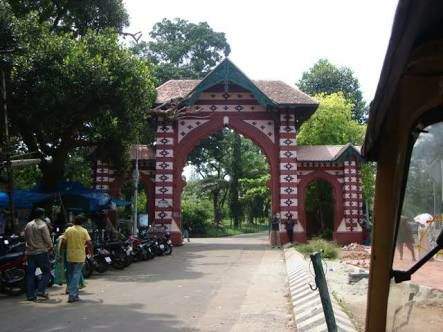
\includegraphics[scale=.45]{images/nada}
\label{nada}
\caption{   }
\end{figure}
  
  . കോർപറേഷൻ ആപ്പിസിൽ വരുന്നവർക്ക് ഹർജി എഴുതിക്കൊടുക്കുക, അകത്ത് ഹർജി എഴുതാനാവശ്യമായ സാമഗ്രികൾ സംഘടിപ്പിക്കുക , ദക്ഷിണ കൃത്യമായി എത്തേണ്ട സ്ഥലങ്ങളേക്കുറിച്ച് ജനങ്ങൾക്കിടയിൽ അവബോധം സൃഷ്ടിക്കുക തുടങ്ങിയ ജനസേവന പ്രവർത്തനങ്ങൾ നടത്തിയായിരുന്നു അമ്മാവൻ കാലം കഴിച്ചിരുന്നത്. അമ്മാവന്റെ കയ്യക്ഷരത്തിൽ ഒരു ഹർജി എഴുതപ്പെട്ടാൽ ഹർജിക്കാരൻ വേറൊരു വഴിയും നോക്കേണ്ടതില്ല കാര്യം നടന്നിരിക്കും. ഇതിന് നിരവധി സാക്ഷ്യങ്ങളുണ്ട്. നല്ല കയ്യക്ഷരത്തിലുള്ള അമ്മാവന്റെ ഹർജി കണ്ട് യുവരാജാവ് പട്ടും വളയും കൊടുത്തു എന്നു വരെ കരക്കമ്പിയുമുണ്ട്. ജോലിക്ക് കൃത്യം കൂലി അമ്മാവന്റെ പോളിസി ആയിരിന്നു. അത് ദ്രവ്യമായോ ദ്രാവകമായോ സ്വീകരിക്കും. ഒസിയാറായിരുന്നു അമ്മാവന്റെ ഇഷ്ട പാനിയം അതും വൈകിട്ട് മാത്രം. ജോലിക്കിടയിൽ അലമ്പില്ല. സ്ത്രികളോടും കുട്ടികളോടും പ്രത്യേക പരിഗണന. ഇങ്ങനെ അമ്മാവൻ കോർപറേഷനാപ്പീസ് ഭരിച്ചിരുന്ന സമയത്ത് ഒരാൾ ഫീസിന് പകരം കാലത്തെതനെ ഒരു പൈൻറ് ഒ സി ആർ അമ്മാവനു സമ്മാനിക്കുകയും അയാളുടെ നിർബന്ധം കാരണം അമ്മാവൻ അപ്പോൾത്തന്നെ കുപ്പി കാലിയാക്കുകയും ചെയ്തു. പ്രതി അമ്മാവന്റെ ഒര കന്ന ബന്ധുവാണെന്നും പറയുന്നുണ്ട്. 
  
  എന്തു പറയേണ്ടു തുടർന്നെഴുതിയ ഹർജികളിൽ അക്ഷരത്തെറ്റ് കടന്നു കൂടുകയും കക്ഷികളുടെ താൽപര്യങ്ങൾക്ക് വിപരീതമായി ഉത്തരവുകളുണ്ടാവുകയും ചെയ്തു. ഇതറിഞ്ഞ അമ്മാവൻ മനോവേദന കൊണ്ട് നീറുകയും മേയറെ സമീപിച്ച് ഉചിതമായ ശിക്ഷ ആവശ്യപ്പെടുകയും ചെയ്തു. മേയറാകട്ടെ അമ്മാവനെ ശിക്ഷിക്കാൻ വിസമ്മതിച്ചു. മനോവിഷമം കൂടിയ അമ്മാവൻ ഒരു ഫുൾ ഓസി ആർ ഒറ്റയടിക്കകത്താക്കി. പിറ്റേന്ന് കാലത്ത് മെഡിക്കൽ കോളേജിൽ വെച്ച് അന്തരിച്ചു. ഇതിനെത്തുടർന്ന് തിരുവനന്തപുരത്ത് അനിഷ്ട സംഭവങ്ങൾ പെട്ടെന്ന് കൂടി . രാജകുടുംബാഗംങ്ങളിൽ ചിലർക്ക് ഡങ്കിപ്പനി, കൗൺസിലർമാരിൽ ചിലർക്ക് കണ്ണിൽ ദീനം ,പോലിസുകാർക്ക് വ്യാപകമായ ജലദോഷം തുടങ്ങി പല ജാതി അസൗകര്യങ്ങൾ ജനങ്ങൾക്കുണ്ടായി. ജനങ്ങൾ പരിഭ്രാന്തരാകാതിരിക്കുമോ. മേലാവിലേക്ക് ഹർജി പോയി. ഇതേത്തുടർന്ന് സർക്കാർ പ്രമുഖ ജോത്സ്യൻമാരുടെ യോഗം വിളിച്ച് പരിഹാരം നിർദേശിക്കാൻ ആവശ്യപ്പെട്ടു.
  
  
   അക്കാലത്തെ പ്രമുഖ യുവ ജോത്സ്യനായിരുന്ന ഡോ. കോട്ടുകാൽ സന്താന കൃഷ്ണൻ അമ്മാവന്റെ ആത്മാവിനെ സെക്രട്ടറിയേറ്റ് നടയിലുള്ള ഒരു ബാറിന്റെ കൗണ്ടറിനടിയിൽ നിന്ന് ആ വാ ഹിച്ചെടുത്തു. ഈ ആത്മാവിനെ ഒരു ഓസി ആർ കുപ്പിക്കുള്ളിലാക്കി കോർപ്പറേഷനാപ്പിസി ന്റെ എതിർവശത്ത് സ്ഥിതി ചെയ്യുന്ന മ്യൂസിയത്തിന്റെ പ്രധാന ഗേറ്റിനോട് ചേർന്ന് പ്രതിഷഠിച്ചു. ഭക്തജനങ്ങൾക്ക് അ മ്മാവനെ വണങ്ങാൻ ചെറിയ ഒരു ഗേറ്റും പണിയിച്ചിട്ടുണ്ട്. ഇക്കാലത്ത് ഈ ഗേറ്റ് മിക്കപ്പോഴും പൂട്ടിയാണിട്ടിട്ടുള്ളത് . പോലിസ് കാവലും ഉണ്ട്. ഈ ഗേറ്റ് തുറന്നാൽ അമ്മാവൻ ചാടിപ്പോയേക്കുമോ എന്ന ഭയമുള്ളതുകൊണ്ട് ഭക്തർ അതാവശ്യപ്പെടാതിരിക്കുന്നതാണ് നല്ലത്. നിങ്ങൾ എന്തെങ്കിലും കാര്യസാധ്യത്തിനായി തിരുവനന്തപുരത്ത് വന്നാൽ നടത്തേണ്ട കാര്യം നല്ലമേനിക്കടലാസിൽ എഴുതി അമ്മാവന്റെ നടക്ക് വെച്ച് പ്രാർത്ഥിക്കുക . ഫലം ഉറപ്പാണ്.
   
    സിനിമാ നടൻമാർ വക്കീലൻമാർ പ്രതികൾ, ജാമ്യക്കാർ, ജഡ്ജിമാർ തുടങ്ങി ജീവിതത്തിന്റെ നാനാതുറയിലുള്ള മലയാളികളുടെയും ഹർജികൾ നടത്തിക്കൊടുക്കുക എന്നതാണ് അമ്മാവൻ പ്രതിഷ്ഠയുടെ ഉദ്ദേശം. PS: .ജീവിച്ചിരിക്കുന്നതോ മരിച്ചതോ ആയ ജഡ്ജിമാരുമായി ഈ ഐതീഹ്യത്തിന് ബന്ധമില്ല. :D
  
  
  \chapter{Education}
    \section{മക്കളെ കമ്പ്യൂട്ടർ പഠിപ്പിച്ചതെങ്ങിനെ ?}
        Audio ready. To be converted to text and corrected. Add lakshmi's interview.
        
    \section{പ്രൊഫസർ വാൾട്ടർ ലെവിന്റെ ഫിസിക്സ് ലക്ചറുകൾ}
    To be rewritten 
    
    ഫിസിക്സ് എൻജിനിയറിംഗ് മറ്റനുബന്ധ ശാസ്ത്ര വിഷയങ്ങൾ പഠിക്കുന്ന വിദ്യാർത്ഥികൾ കണ്ടിരിക്കേണ്ട ഒന്നാണ് പ്രൊഫസർ വാൾട്ടർ ലെവിന്റെ ഫിസിക്സ് ലക്ചറുകൾ. ഈ ലക്ചറുകൾ എം ഐ ടി യു ടെ O C W പ്രോഗ്രാമിലെ ഏറ്റവും പോപ്പുലറായ കോഴ്സുകളിലൊന്നായിരുന്നു എന്നാൽ പ്രൊഫസർ ലെവിൻ നേരിട്ട ചില ആരോപണങ്ങളെത്തുടർന്ന് ocw ഇത് അവരുടെ സൈറ്റിൽ നിന്ന് നീക്കം ചെയ്തു. ക്രിയേറ്റിവ് കോമൺസ് ലൈസൻസുള്ള ഈ ലക്‌ചറുകൾ എല്ലാം ഇപ്പോൾ യൂട്യൂബിൽ ലഭ്യമാണ്‌. YouTube ൽ physics 8.01 എന്ന് സെർച്ച് ചെയ്താൽ ഇത് കിട്ടും. OCWവിൽ വിഡിയോ ലക്ചറുകൾക്ക് പുറമെ അനുബന്ധ പഠനസാമഗ്രികളും ലഭ്യമായിരുന്നു. അതൊന്നും ഇപ്പോൾ എവിടെയും കാണുന്നില്ല. 
    
    %https://en.m.wikipedia.org/wiki/Walter_Lewin ഇദ്ദേഹത്തിന്റെFor the love of physics എന്ന ബെസ്റ്റ് സെല്ലർ ആ മസോണിലുണ്ട്. ക്ലാസ് മുറിയെ പരിക്ഷണശാലയാക്കിക്കൊണ്ട് പ്രൊ. ലെവിൻ നടത്തുന്ന ക്ലാസുകൾ ഏതൊരു ശാസ്ത്ര വിദ്യർത്ഥിയേയും ആകർഷിക്കും. ഇതാ ചില സാമ്പിൾ ക്ലാസ് റൂം പരീക്ഷണങ്ങൾ. ഫിസിക്സിനെ വിശ്വസിക്കാമോ എന്ന പാഠം കണ്ടു നോക്കു. https://youtu.be/xXXF2C-vrQE ന്യട്ടന്റെ ചലന നിയമങ്ങൾ എങ്ങിനെയാണ് പഠിപ്പിക്കേണ്ടതെന്ന് കാണുക. https://youtu.be/dv-mXAhhWG0 MIT യിൽ നിന്ന് വിരമിച്ചപ്പോൾ ലെവിൻ നടത്തിയ ലാസ്റ്റ് ലക്ചർ ഒരു ക്ലാസിക്കാണ്. കാണാൻ മറക്കണ്ട. https://youtu.be/4a0FbQdH3dY Thanks to എൽദോ ദാനിയൽ for reminding me about the course that I watched long back. Edit: Course material is here https://web.archive.org/web/20140711022414/http://ocw.mit.edu/courses/physics/8-01-physics-i-classical-mechanics-fall-1999/download-course-materials/
    
    \section{തപാൽ വഴി നീന്തൽ }
    
    തപാൽ വഴി നീന്തൽ പഠിക്കുന്നതാണല്ലോ ഫാഷൻ. ഞാൻ തപാൽ വഴി നീന്തൽ പഠിച്ച കഥ പറയാം. 2010ലാണ് ഐ ഐ ടി ബോംബെയിൽ എത്തിപ്പെടുന്നത്. ആദ്യ വർഷം രണ്ടു മാസമേ അവിടെ നിന്നുള്ളു QIP (ഇത് കേന്ദ്ര സർക്കാരിന്റെ കോളേജ് വാധ്യാന്മാരുള്ള ഒരു വയോജന വിദ്യാഭയസ പരിപാടിയാണ് ) ക്കാർക്ക് ബോംബെ ശീലങ്ങൾ പഠിക്കാനുള്ള ഒറിയന്റേഷൻ കാലമാണ് ആ രണ്ട് മാസം . ആകെ ജോളിയടിച്ച് നടന്നു. 2011 ൽ ആണ് ശരിക്ക് Ph Dവർക്ക് തുടങ്ങിയത്.M Tech കഴിഞ്ഞിട്ട് 10 വർഷം കഴിഞ്ഞിരുന്നു. ആ പത്തു വർഷവും പുസ്തകം കൈ കൊണ്ടു തൊട്ടിട്ടില്ല എന്ന് പറയാം. PhDതുടങ്ങുമ്പോൾ കുറെ കോഴ്സ് കൾ ചെയ്യണം. അവരവരുടെ റിസർച്ച് ടോപ്പിക്കിനനുസരിച്ച് സൂപർ വൈസർ ഏതൊക്കെ കോഴ്സ് വേണമെന്ന് നിശ്ചയിക്കും. എനിക്ക് കിട്ടിയത് പ്രോബബിലിറ്റി തിയറി, ലീനിയർ ഒൾ ജിബ്രാ, ഇമേജ് പ്രോസസിംഗ്, മെഷിേൻലേർണിഗ് എന്നിവ. ഒരാഴ്ചകൊണ്ട് ഒരു കാര്യം മനസ്സിലായി കോഴ്സ് 8 നിലയിൽ പൊട്ടും. കുട്ടാനും കുറക്കാനുമല്ലാതെ കണക്ക് സാറൻ മാർ പഠിപ്പിച്ചതൊന്നും ഓർമ്മയില്ല. ഒന്നാമത്തെ സീരിസ് മനോഹരമായി തോറ്റു.മാർക്കൊക്കെ സിംഗിൾ ഡിജിറ്റ്. അങ്ങനെ വിഷണ്ണനായിരിക്കുമ്പോഴാണ് ഖാൻ അക്കാദമി കണ്ണിൽപ്പെട്ടത്. സായ് ഖാൻ എന്ന പാക്കിസ്ഥാനി എൻജിനിയർ സഹോദരിയെ കണക്ക് പഠിപ്പിക്കാനായി തുടങ്ങിയ ഓൺലൈൻ പാoങ്ങളാണ് ആദ്യം ഉണ്ടായിരുന്നത്. നല്ലവണ്ണം മിനക്കെട്ട് പ്രീ ഡിഗ്രി ക്കൊക്കെ പഠിച്ച കണക്ക് ഒന്നു കുടി ഖാനക്കാഡമിയിൽ നിന്ന് പഠിച്ചു.

%\begin{verbatim}
  
%     https://www.khanacademy.org/math പിന്നെ കോഴ്സറ എഡ്എക്സ് ഉഡാസിറ്റിയിലൊക്കെ വരുന്ന കോഴ്സുകൾക്കൊക്കെ ചറപറ രജിസ്റ്റർ ചെയ്യും.പലതും രണ്ടും മൂന്നും ആഴ്ച കാണും. നിറുത്തും. ഇതിനിടയിൽ ചിലതൊക്കെ പൂർത്തിയാക്കുകയും ചെയ്തു. ഇങ്ങനെ ചെയ്ത കോഴ്സുകളിൽ എനിക്ക് എറ്റവും ഇഷ്ടപ്പെട്ട ചിലത് താഴെ കൊടുക്കുന്നു. 1) കാൽക്കുലസ് സിംഗിൾ വേരിയബിൾ https://www.coursera.org/learn/single-variable-calculus ഗണിതം എൻജിനിയറിംഗ് ഫിസിക്സ് എന്നി വിഷയങ്ങൾ പഠിക്കുന്നവർ, ( പഠിച്ചു കഴിഞ്ഞവരും) ഉറപ്പായും കണ്ടിരിക്കേണ്ടതാണ്. കണക്കു ക്ലാസുകൾ എങ്ങിനെ നടത്തണമെന്നതിന്റെ ഉദാഹരണം കൂടിയാണ് പെൻസിൽവേനിയ യൂണിവേർസിറ്റിയുടെ ഈ കോഴ്സ്. 2) പ്രോബബിലിറ്റി. സന്തോഷ് വെങ്കടേഷ് എന്ന ഇന്ത്യൻ പ്രൊഫസറുടെ ഗംഭീര ക്ലാസ്. ഗണിത വിദ്യാർത്ഥികൾ ഉറപ്പായും കാണണം ഇത് ഇപ്പോൾ ഓൺലൈനിൽ കാണുന്നില്ല. യുട്യൂബിൽ ഒരു ട്രൈലെർ ഉണ്ട് https://www.youtube.com/watch?v=AuoTfIcFQgU 3) ലീനിയർ ഒൾജിബ്ര ഗിൽബർട്ട്സ്ട്രാംഗ്. മെട്രിക് സ് എന്താണെന്നും എന്തിനാണെന്നും ഞാൻ പഠിച്ചത് ഇതുകണ്ടാണ്. https://ocw.mit.edu/faculty/gilbert-strang/ 4) മെഷിൻ ലേ ർ ണി ഗ് ആൻഡ്രു ഇങ്ങ്. തുടക്കക്കാർക്ക് അത്യുത്തമം. https://www.coursera.org/learn/machine-learning 5) പ്രൊഫസർ വിക്രം ഗദ് രെ ബോംബെ ഐഐടിയിലെ കിടിലൻ പ്രൊഫസറാണ്. ഇദ്ദേഹത്തിന്റെ ഡി എസ് പി വേവ് ലെറ്റ് ക്ലാസുകളിൽ ഇരുന്നിട്ടുണ്ട്. എഡ് എക്സിൽ ഇദ്ദേഹത്തിന്റെ സിഗ്നൽ സ് ആന്റ് സിസ്റ്റംസ് എന്ന കോഴ്സുണ്ട്. എൻജിനിയറിംഗ് ചെയ്യുന്നവരെല്ലാം ആവശ്യം കണ്ടിരിക്കേണ്ടതാണി കോഴ്സ്. വേവ് ലെറ്റ് ഡി എസ് പി എന്നി കോഴ്സുകൾ യൂട്യൂബിൽ കിട്ടാനുണ്ട്. ഈ വിഷയത്തിൽ ഐ ഐ ടി ഡെൽഹിയിലെ ദത്താ റോയിയുടെ ക്ലാസുകളും നല്ലതാണ്. https://iitbombayx.in/courses/IITBombayX/EE210.1x/2015-16/about മുകളിൽ പറഞ്ഞവയെല്ലാം ഞാൻ കംപ്ലിറ്റ് ചെയ്തവയാണ്. പകുതി വെച്ചു നിറുത്തിയവ ചിലത്. ഇവ ഇനിയും ചെയ്യണമെന്നുണ്ട്. 1) യുവാൽ ഹരാരി. ഇത് ഇപ്പോൾ കോഴ്സറായിൽ കാണാനില്ല. https://www.youtube.com/watch?v=sGdMBqDPB1A 2 മാത്തമാറ്റിക്കൽ തിങ്കിംഗ് https://www.coursera.org/learn/mathematical-thinking 3) ഒഡിയോസിഗ്നൽ പ്രോസസിംഗ്. https://www.coursera.org/learn/audio-signal-processing പ്രൊഫസർ സേവർ സേരയുടെ കിടിലൻ കോഴ്സാണ്. ഇതു കണ്ടിഷ്ടപ്പെട്ടിട്ട് സേവ്യർ സേ ര IISc യിൽ വന്നപ്പോൾ രണ്ടു ദിവസത്തേ കോഴ്സിനു ലിവെടുത്ത് പോയി. 4 ബിറ്റ്കോയിൻ ടെക്നോളജി സ് https://www.coursera.org/learn/cryptocurrency ഇത് പകുതി കണ്ടു. അസൈൻമെന്റ് ചെയ്യാൻ പറ്റിയില്ല. 5 നാൻഡ് ടു ടെട്റിസ് https://www.coursera.org/learn/build-a-computer കമ്പ്യൂട്ടർ സയൻസ് വിദ്യാർത്ഥികൾ ഇതു ഉറപ്പായും കാണണം. 2011 - I 4 കാലത്താണ് പിഎച്ച്ഡി വർക്ക് പ്രധാനമായും നടന്നത്. ഓൺലൈൻ കോഴ്സുകൾ ഓരോ സ്റ്റേജിലും സഹായിച്ചിട്ടുണ്ട്‌. ഇവയൊക്കെപുസ്തകം വായിച്ചു പഠിക്കാനെടുക്കുമായിരുന്നതിന്റെ പത്തിലൊന്നു സമയമേയെടുത്ത കാണു . വാൽക്കഷണം: ഈയടുത്ത് KTU വിന്റെ MCA സിലബസ് നിശ്ചയിക്കുന്ന കമ്മറ്റിയിൽ അംഗമായിരുന്നു. ഓരോ വിഷയത്തിനുമൊപ്പം റഫറൻസ് ആയി ഒന്നോരണ്ടോ M00C കുടികൊടുക്കണമെന്ന് ഞാൻ ഒരു നിർദ്ദേശം വെച്ചു. അതു പ്രകാരം ഉണ്ടാക്കിയ സിലബസ് ആണ് ഇത്. https://ktu.edu.in/data/MCA_Regular_First_To_Fourth_Semester_Syllabus_Final.pdf ഇതിനുവേണ്ടി കുറെ മുക്കുകൾ കാണെണ്ടിവന്നു. എത്രമാത്രം എഫക്ടീവാണ് ഈ നിർദേശമെന്ന് കണ്ടറിയണം. ചില തിന്റെയൊക്കെ ലിങ്ക് മാറി എന്നൊക്കെ പരാതി വന്നു. ആരൊക്കെയോ ഉപയോഗിക്കാൻ നോക്കിയതുകൊണ്ടാണല്ലോ പരാതി വന്നത്. അപ്പൊ എല്ലാരും മുരളിച്ചേട്ടൻ പറഞ്ഞതുപോലെ വെള്ളത്തിലോട്ടു ചാടിക്കോ .
     
     
%\end{verbatim}  
\section{NUMATS}
നമ്മുടെ പൊതു വിദ്യാഭ്യസ വകുപ്പ് innovative ആയ പല പദ്ധതികളും നടത്തന്നുണ്ട്.. കുട്ടികളുടെ യി ടയിലും അധ്യാപകരുടെയിടയിലും വേണ്ടത്ര അവബോധമില്ല എന്നത് പലപ്പോഴും ഇത്തരം പദ്ധതികൾ പരിപൂർണ വിജയത്തിലെത്തുന്നതിന് തടസമാണ്. ഗണിത ശാസ്ത്ര പ്രതിഭകളെ പ്രോത്സാഹിപ്പിക്കുന്നതിനുള്ള Num ATs അത്തരം ഒരു പദ്ധതിയാണ്. ആറാം ക്ലാസിൽ പഠിക്കുന്ന കുട്ടികൾക്ക് സംസ്ഥാന വ്യാപകമായി നടത്തുന്ന ഒരു പൊതു പരീക്ഷയോടെയാണ് ഇത് തുടങ്ങുന്നത്. ഇതിന് ശേഷം ഓരോ ജില്ലയിൽ നിന്നും അഞ്ചു പേരെ വീതം തിരഞ്ഞെടുക്കും.അവർക്ക് അടുത്ത അഞ്ചു വർഷത്തേക്ക് അവധിക്കാല ഗണിത ക്യാമ്പും മറ്റു തുടർപ്രവർത്തനങ്ങളുമാണ് നടത്തുന്നത്. തെക്കൻ ജില്ലകളിലെ കുട്ടികൾക്കുള്ള ഈ വർഷത്തെ തുടർ പ്രവർത്തനം ഇന്ന് ചെങ്ങന്നൂർ ബോയ്സ് ഹൈസ്കൂളിൽ വെച്ച് നടക്കുന്നു. ക്യാമ്പിൽ വിദ്യയും കീർത്തിയും പങ്കെടുക്കുന്നതിനാൽ ഇന്ന് എസ് കോർട്ട് ഡ്യൂട്ടിയാണ്.. കഴിഞ്ഞ അഞ്ചു വർഷമായി വിദ്യ ക്യമ്പിൽ ഉണ്ട്. കഴിഞ്ഞ വേനൽക്കാല ക്യാമ്പുതൊട്ട് കീർത്തിയും. ഇവിടെ കൊടുക്കുന്ന ചോദ്യങ്ങൾ ശരിക്കും ചലഞ്ചിങ്ങ് ആണ്. 7 ലെ ക്കൊടുത്തിട്ടുണ്ട്. താൽപര്യമുള്ളവർക്ക് ശ്രമിക്കാം. കുട്ടികൾക്ക് സംസ്ഥാനത്ത് ഉടനീളം വലിയ ഒരു സുഹൃത് വലയം കിട്ടിയെന്നുള്ളത് ക്യാമ്പിന്റെ മറ്റൊരു ഗുണഫലമാണ്. 
%http://www.scert.kerala.gov.in/index.php?option=com_content&view=article&id=110&Itemid=93
 കഴിഞ്ഞ അഞ്ചു വർഷം ഈ പദ്ധതിയെ പുറത്തു നിന്ന് നിരീക്ഷിച്ചതിൽ നിന്ന് ചില കാര്യ ങ്ങ ൾ . പല സ്കൂളുകളും ഈ പദ്ധതി വേണ്ടത്ര ശ്രദ്ധയോടെ നടത്തുന്നില്ല. കീർത്തി പരീക്ഷയെഴുതിയ തിരുവനന്തപുരം സബ് ജില്ലയിലെ പരീക്ഷാ നടത്തിപ്പും participation ഉം പരിതാപകരമായിരുന്നു പദ്ധതി നടത്തിപ്പ് പലപ്പോഴും കുട്ടികൾക്കും രക്ഷിതാക്കൾക്കും ബുദ്ധിമുട്ടുണ്ടാക്കുന്ന രീതിയിലാന്ന്. ഇന്നത്തെ ക്യാംപിന്റെ വിവരം ഇന്നലെ അറിയിക്കുന്നത് നന്നല്ല.സ്കൂൾ അടങ്ങുന്നതിന് മുമ്പ് പ്രവർത്തനങ്ങൾ പ്ലാൻ ചെയ്ത് രക്ഷകർത്താക്കളെ അറിയിക്കണം. ക്യാമ്പിൽ പങ്കെടുക്കുന്ന വിദഗ്ദർ ആരൊക്കെയാണ് എന്താണ് പ്രവർത്തനങ്ങൾ എന്നൊക്കെ രക്ഷകർത്താക്കളെ അറിയിച്ചാൽ നന്ന്. റസിഡൻഷ്യൽ ക്യാംപ് നല്ല സ്ഥലസൗകര്യമുള്ള സ്കൂളുകളിലാണ് സംഘടിപ്പിക്കേണ്ടത് ( ധ്യാനകേന്ദ്രങ്ങളിലല്ല.:D) ക്യാംപ് നടത്തിപ്പുകാരെ ഗവർമെണ്ട് മാറുന്നതനുസരിച്ച് മാറ്റരുത് ഒരു ടീമിനെ കുറഞ്ഞത് മൂന്ന് വർഷത്തേക്കെങ്കിലും ചുമതല ഏൽപിക്കണം. മൊത്തത്തിൽ നോക്കിയാൽ ക്യാമ്പ് വളരെ നല്ലതാണ്. മറ്റ് വിഷയങ്ങൾക്കും ഇത്തരം ക്യാമ്പുകൾ നടത്താവുന്നതാണ്. IT ,ഫിസിക്സ് മലയാളം തുടങ്ങിയക്കൊക്കെ ക്യാമ്പ്യകൾ വരട്ടെ. PS: പദ്ധതി പൊതു വിദ്യാലയങ്ങളിലെ കുട്ടികൾക്ക് മാത്രം.
 \section{  പാഠപുസ്തക പരിഷകരണം }
    പാഠപുസ്തക പരിഷകരണം വീണ്ടും നടത്താൻ പോകുന്നുണ്ടെന്ന് തോന്നുന്നു .കമ്മിറ്റിയിൽ കയറാൻ പറ്റാത്തതിന്റെ വിഷമം ഇന്നത്തെ പത്രത്തിലുണ്ട്. എന്റെ മൂന്ന് മക്കളും സർക്കാർ സ്കൂളിലാണ് പഠിക്കുന്നത് .ഒരു രക്ഷകർത്താവെന്ന നിലയിലുള്ള അഭിപ്രായമാണ്. (സർക്കാരുമായി ജഗഡ ഇല്ല.:D ) എന്റെ ഓർമയിൽ മലയാള പാഠാവലി ഒരു അഞ്ചു തവണയെങ്കിലും പരിഷ്കരിച്ചിട്ടുണ്ട്. ഞാൻ പഠിച്ച പുസ്തകത്തിൽ റാകിപ്പറക്കുന്ന ചെമ്പരുന്തേ എന്നു തുടങ്ങുന്ന രണ്ടു വരി കവിതയുണ്ടായിരുന്നു. ഒരിടക്ക് മന്ത്രി ടി എം ജേക്കബ് ചൈനയിലോ മറ്റോ പോയി വന്നു. തുടർന്ന് ചെമ്പരുന്തി നേക്കുറിച്ച് ഒരു വിവാദമൊക്കെ ഉണ്ടായി.ഇതിനെത്തുടർന്ന് ടി എം ജേക്കബിന്റെ കാലത്തു തന്നെ ഈ പുസ്തകം മാറ്റി പുതിയത് വന്നു. പിന്നാലെ വന്ന സർക്കാർ പുസ്തകം വീണ്ടും മാറ്റി. തുടർന്ന് ഓരോ തവണ സർക്കാർ മാറുമ്പോഴും പുസ്തകം മാറും എന്ന സ്ഥിതിയായി. പുസ്തകക്കമ്മറ്റിയിൽ സ്വന്തക്കാരെ വെച്ച് എന്തെങ്കിലും കാട്ടിക്കുട്ടി. സർക്കാർ പള്ളിക്കൂടത്തിലെ പിള്ളേർക്ക് ഇതൊക്കെ മതി എന്ന രീതിയായി മാറി. കഴിഞ്ഞ വർഷം അഞ്ചാം ക്ലാസിൽ പഠിപ്പിച്ച കാര്യം ഇത്തവണ ഒൻപതിലായി. അതിന്റെയൊക്കെ പരിണിത ഫലമാണ് പത്ത് കഴിഞ്ഞ ആർക്കും നേരെ ചൊവ്വെ എഴുത്തും വായനയും അറിയാത്തത്. എന്റെ അഭിപ്രായത്തിൽ പാo പുസ്തക പരിഷ്കരണം ഇൻക്രിമെൻറ ലായെ നടത്താവു. ഈ വർഷത്തെ പുസ്തകത്തിന്റെ കുഴപ്പം കണ്ടെത്തി അതു പരിഹരിക്കണം അല്ലാതെ വീണ്ടും പുതിയതെഴുതരുത്. ഇപ്പോൾ നിലവിലുള്ള പാഠപുസ്തകങ്ങൾ മുഴുവൻ ഒരു വിക്കിയിലാക്കട്ടെ. പൊതുജനങ്ങളുടേയും അധ്യാപകരുടെയും അഭിപ്രായങ്ങൾ കമൻറുകളായി വരട്ടെ. എന്നിട്ട് സമയമെടുത്ത് പുസ്തകം പരിഷ്കരിക്കട്ടെ .
    
    \section{ ചോദ്യപ്പേപ്പറിൽ ഇംഗ്ലീഷ്}
    മലയാളം ചോദ്യപ്പേപ്പറിൽ ഇംഗ്ലീഷ് അച്ചടിച്ചു എന്ന് ഏതോ മ. ചാനൽ വിളിച്ചു കൂവുന്നുണ്ടല്ലോ. ഈ സന്ദർഭത്തിൽ ഭാഷാ പഠനത്തേക്കുറിച്ച് ചില കാര്യങ്ങൾ കുറിക്കട്ടെ. കേരളത്തിൽ സ്കൂൾ ക്കുട്ടികൾ മൂന്ന് ഭാഷകളാണ് ഇപ്പോൾ പഠിക്കുന്നത്. ഇംഗ്ലീഷ് മലയാളം ഹിന്ദി എന്നിവ. ഒന്നാമതായി ആലോചിക്കേണ്ടത് കുട്ടികൾ മൂന്ന് ഭാഷ പഠിക്കേണ്ടതുണ്ടോ എന്നാണ്. നമ്മുടെ സ്കൂളിൽ നിന്ന് +2 പാസായ ഏതെങ്കിലും കുട്ടി ഹിന്ദി സംസാരിക്കുമോ. ഇല്ല എന്നാണ് എനിക്ക് തോന്നിയിട്ടുള്ളത്. കുട്ടികൾ അൽപമെങ്കിലും ഹിന്ദി മനസ്സിലാക്കുന്നുണ്ടെങ്കിൽ വല്ല സീരിയലും കണ്ടിട്ടാകും. പിന്നെ എന്തിനാണ് കുട്ടികളെ ഹിന്ദി പഠിപ്പിക്കുന്നത്. കുട്ടികളെ ഒന്നാം ക്ലാസ് മുതൽ ഹിന്ദി പഠിപ്പിക്കുന്ന പരിപാടി നിറുത്താറായി (ഹിന്ദി സാറൻമാർ ദേശിയ വാദികൾ നാടൻ ഗോസായി മാർ എന്നിവർ പൊങ്കാല ഇടുന്നുണ്ടെങ്കിൽ ദയവായി ഹിന്ദിയിൽ മാത്രമിടുക.:D ) ഫ്രെഞ്ച് ജർമ്മൻ തുടങ്ങിയ ഭാഷകൾ ചില സ്കൂളുകളിൽ 11 ാം ക്ലാസിൽ പഠിപ്പിക്കുന്നുണ്ട്. ഹിന്ദിയും അത്രയേ വേണ്ടു. അത്യാവശ്യം അക്ഷരമാലയും അഞ്ചാറ് വാക്കുകളും പഠിക്കട്ടെ. അല്ലാതെ സൂർ ദാസിന്റെ കവിതയും പ്രേം ചന്ദിന്റെ കഥയും പഠിപ്പിച്ച് ആളെ വെറുപ്പിക്കരുത്. ഇന്ന് ജീവിച്ചിരിക്കുന്ന മലയാളികൾ മിക്കവരും പത്തു വരെയെങ്കിലും ഹിന്ദി പ ഠിച്ചവരാണ്. ഇതിലെ ബഹു ഭൂരിപക്ഷത്തിനും ഹിന്ദി അക്ഷരമാല മുഴുവൻ അറിയാമോ എന്ന് സംശയമാണ്. ഇനി ഇംഗ്ലീഷിന്റെയും മലയാളത്തിന്റെയും കാര്യമെടുക്കാം. എന്റെ അഭിപ്രായത്തിൽ കുട്ടികളെ പഠിപ്പിക്കേണ്ടത് functional language ആണ്. സ്വന്തം ആശയങ്ങൾ വ്യക്തമായി പ്രകടിപ്പിക്കുന്നതിനും മറ്റുള്ളവരുടെ ആശയങ്ങൾ വായിച്ചും കേട്ടും മനസ്സിലാക്കുന്നതിനു മുള്ള കഴിവാണ് +2 വരെയുള്ള കുട്ടികൾക്ക് ഉണ്ടാക്കി കൊടുക്കേണ്ടത്. ഇപ്പോഴത്തെ ഭാഷാ പാഠപുസ്തകങ്ങൾ എല്ലാം തന്നെ കുട്ടിയെ സാഹിത്യാസ്വാദകനാക്കാനാണ് ശ്രമിക്കുന്നത്. പത്താം ക്ലാസിലെ കുട്ടിയെ നളചരിതവും കട്ടക്കയത്തിൽ ചെറിയാൻ മാപ്പിളയുടെ ശ്രീയേശു വിജയവും ഉരുവിട്ടു പഠിപ്പിക്കാൻ ശ്രമിക്കുന്നത് പരമാബദ്ധമാണ്. എന്റെ അഭിപ്രായത്തിൽ ഇംഗ്ലീഷ് പരീക്ഷയും മലയാളം പരീക്ഷയും കുട്ടിക്ക് ചോദ്യപ്പേപ്പറിൽ പറഞ്ഞിരിക്കുന്ന ആശയം മനസ്സിലായോ എന്നാണ് പരിശോധിക്കേണ്ടത്. ഇംഗ്ലീഷൽ എഴുതിയ കാര്യം മനസിലാക്കി കുട്ടി ഉത്തരം മലയാളത്തിലെഴുതട്ടെ. തിരിച്ചും . കൂടാതെ തെറ്റുകൂടാതെ ഇംഗ്ലിഷും മലയാളവും പറഞ്ഞ് ഫലിപ്പിക്കുവാനാകുമോ എന്നും പരിശോധിക്കണം. ഇംഗ്ലീഷിൽ എഴുതിയിരിക്കുന്ന കാര്യം വ്യക്തതയോടെ മനസ്സിലാക്കേണ്ടത് ആധുനിക യുഗത്തിൽ അതിജീവനത്തിന് അത്യന്താപേക്ഷിതമാണ്. അതിനാൽ വിവാദ ചോദ്യത്തിന്റെ മാതൃകയിൽ കൂടുതൽ ചോദ്യങ്ങൾ വരട്ടെ വിവാദ ചോദ്യത്തിന്റെ താഴെയുള്ള ചോദ്യങ്ങൾ നോക്കുക. ഏതെങ്കിലും ഗൈഡ് നോക്കി കാണാതെ പഠിച്ചിട്ടാകും സാഹിത്യാഭിരുചിയില്ലാത്ത ഭൂരിപക്ഷവും എഴുതുക. ഇന്നു പരിക്ഷയെഴുതിയ കുട്ടിയോട് ഒരാഴ്ച കഴിഞ്ഞ് ബകനേക്കുറിച്ചോ നള നേക്കുറിച്ചോ ചോദിച്ച് നോക്ക് അപ്പോഴറിയാം ഇപ്പോഴത്തെ ഭാഷാ പഠന രീതിയുടെ ഗുണം.
  \section{പാലായും പാറ്റ്നയും}
   ഇന്നത്തെ ഹിന്ദു പത്രത്തിലെ ഒന്നാം പേജിലെ പരസ്യവും ഏഴാം പേജിലെ വാർത്തയുമാണ് ഈ കുറിപ്പിന് പ്രചോദനം. ഐ ഐ ടി പ്രവേശനപ്പരീക്ഷയുടെ റിസൾട്ട് ഇന്നലെ വന്നു.പാലായിലെ പ്രശസ്ത കോച്ചിംഗ് സെൻറർ അവരുടെ നേട്ടം ഒന്നാം പേജ് പരസ്യമായി ഇട്ടിട്ടുണ്ട്. കേരളത്തിലെ മറ്റ് കോച്ചിംഗ് സ്ഥാപനങ്ങളുടെ പരസ്യങ്ങളൊന്നും കണ്ടില്ല. കോച്ചിംഗ് ഇല്ലാതെ നൂറിൽ താഴെ റാങ്ക് വാങ്ങിയ ഒരു മിടുക്കന്റെ വാർത്ത മൂന്നാം പേജിലുണ്ട്. ഇത്തരക്കാർഇനിയും കുറേ പേർ കൂടി കാണും. ഐ ഐ ടി കളിലെല്ലാം കുടി 11000 ത്തിൽ പരം സിറ്റുകളാണുള്ളത്. ഹിന്ദുവിന്റെ ഒന്നാം പേജിൽ വന്ന പരസ്യപ്രകാരം 10000ത്തിൽ താഴെ റാങ്കുള്ളവർ 280 പേരുണ്ട്.മറ്റു കോച്ചിംഗ് സെന്ററുകളിലെല്ലാം കൂടി ഒരു 50 കൂടിക്കാണും. ഈ കുട്ടികളെല്ലാം തന്നെ നല്ല സാമ്പത്തിക സ്ഥിതിയുള്ളവരായിരിക്കും. ഒരു വർഷത്തെകോച്ചിംഗ് ന് ഒരു ലക്ഷം രൂപ യൊക്കെ ഫിസുണ്ട്. കേരളത്തിൽ നിന്ന് ഐഎ ടി അഡ്മിഷൻ നേടുന്ന വിദ്യാർത്ഥികളുടെ എണ്ണം വടക്കൻ സംസ്ഥാനങ്ങളെ അപേക്ഷിച്ച് വളരെ കുറവാണ്. പെൺകുട്ടികൾ ഇല്ലെന്നു തന്നെ പറയാം. ഇനി പാറ്റ്നയിൽ നിന്നു വന്ന ഏഴാം പേജ് വാർത്ത നോക്കാം.അനന്തകുമാർ എന്നൊരു വ്യക്തി നടത്തുന്ന സൂപ്പർ 30 എന്ന കോച്ചിംഗ് പ്രോഗ്രാമിലെ മുപ്പത് കുട്ടികളും ഐ ഐ ടി പരീക്ഷ ക്വാളിഫൈ ചെയ്തു എന്നാണാ വാർത്ത. സുപ്പർ 30 സമൂഹത്തിലെ താഴെക്കിടയിലുള്ള സാധാരണ മനുഷ്യരുടെ മക്കളെ ഫിസൊന്നും വാങ്ങാതെ ഐ ഐ ടി കോച്ചിംഗ് കൊടുക്കാനുള്ള ഉദ്യമമാണ്. കഴിഞ്ഞ 15 വർഷമായി അനന്തകുമാർ ഈ കോച്ചിംഗ് ക്ലാസ് നടത്തുന്നു. മിക്കവാറും എല്ലാ വർഷവും നൂറ് മേനിയാണ് വിളവ്. ബിഹാറിലെ സാധാരണ മനുഷ്യരുടെ സാമ്പത്തിക / സാമുഹിക സ്ഥിതി നമുക്കറിവുള്ളതാണല്ലോ. പണം മുടക്കാനില്ലാത്തതിനാൽ പഠിക്കാനവസരമില്ലാത്ത മുപ്പതു പേരെ തിരഞ്ഞെടുത്ത് പരിശിലിപ്പിക്കുകയാണ് അനന്തകുമാർ ചെയ്യുന്നത്. സൂപ്പർ 30ന്റയും അനന്തകുമാറിന്റെയും വിക്കി പേജുകൾ താഴെ കൊടുത്തിട്ടുണ്ട്. പൊതു വിദ്യാഭ്യാസത്തെ ശക്തിപ്പെടുത്താൻ ഗവർമെന്റ് നടപ്പാക്കി വരുന്ന പദ്ധതിയുടെ ഭാഗമായി സൂപ്പർ 30 പോലെ ഒരു ശ്രമം കേരളത്തിലും നടത്തേണ്ടതാണ്. സാമ്പത്തിക സ്ഥിതിയില്ലാത്ത മിടുക്കൻമാർക്ക് ഇപ്പോൾ ഐ ഐ ടി പോലെയുള്ള മുൻനിര സ്ഥാപനങ്ങളിലെ പ്രവേശനം അപ്രാപ്യമാണ്. പട്ടികജാതി/വർഗ വിഭാഗത്തിൽ നിന്ന് ഇത്തരം സ്ഥാപനങ്ങളിൽ വളരെ ചുരുക്കം ആളുകളേ എത്തിപ്പെടുന്നുള്ളു. (മുന്നോക്ക /പിന്നോക്ക കോർപറേഷനൊക്കെ ഈ വിഷയത്തിൽ ഇടപെടാനുള്ള വകുപ്പുണ്ട് :D) കേരളത്തിൽ നിന്ന് രാജ്യത്തെ മുൻനിര സ്ഥാപനങ്ങളിൽ കൂടുതൽ പേരെ എത്തിക്കുക എന്നതുകൂടി പൊതു വിദ്യാഭ്യാസ സംരക്ഷണ യജ്ഞത്തിന്റെ ലക്ഷ്യങ്ങളിൽ ഒന്നാകട്ടെ.
   
   % Reference: https://en.m.wikipedia.org/wiki/Super_30 http://www.super30.org https://en.m.wikipedia.org/wiki/Anand_Kumar http://www.thehindu.com/news/national/other-states/iit-jee-examination-results-all-30-students-from-super-30-crack-iit-jee-exam/article18959852.ece
 
   
   \section{ ഏത് കോളേജിലാണ് ചേരേണ്ടത്? }
  അടുത്ത ഒന്നു രണ്ടാഴ്ചക്കുള്ളിൽ എൻട്രൻസ് പരീക്ഷയുടെ ഫലം വരും. കേരളത്തിൽ 160 എൻജിനിയറിംഗ് കോളേജുകളുണ്ട്. അവയിൽ മിക്കതും ആളെ പിടിക്കാൻ വലയുമായി ഇറങ്ങിക്കഴിഞ്ഞു. ചില പരസ്യങ്ങളൊക്കെ കണ്ടാൽ ഫൈവ് സ്റ്റാർ ഹോട്ടലിലാണോ ഇവർ കുട്ടികളെ പഠിപ്പിക്കുന്നത് എന്ന് തോന്നും. പലയിടത്തും ചേർന്നാൽ ഹോട്ടലാണെന്ന് കരുതി ബാർബർ ഷോപ്പിൽ കയറിയതുപോലെയാകും ഫലം. കേരളത്തലെ ഒരു കോളേജും ലോകനിലവാരത്തിലുള്ളതല്ല. എല്ലാവർക്കും വിദേശത്തോക്കെ പോകാനാവില്ലല്ലോ. അതിനാൽ ഉള്ളതിൽ നിന്ന് നിങ്ങൾ ശ്രദ്ധാപൂർവ്വം കോളേജ് തിരഞ്ഞെടുക്കണം. ഓരോ കോളേജും ഓരോecosystem ആണെന്നന്ന് പറയാം. ചിലത് നമ്മുടെ യക്ഷിക്കാവുകളെപ്പോലെ ജൈവവൈവിധ്യമുള്ളത് ,മറ്റു ചിലത് അത്യ ൽപാദന ശേഷിയുള്ള റബർ എസ്റ്റേറ്റുപോലെയും. എവിടെ ചേർന്നാലും നിങ്ങൾക്ക് ഡിഗ്രി കാട്ടാൻ സാധ്യതയുണ്ട്.കാവി ലൊക്ക നല്ല വിഷമുള്ള മൂർഖൻ പാമ്പുകളൊക്കെ കാണും. സൂക്ഷിച്ച് നടന്നാൽ ജീവിതത്തിന്റെ ഗതി തന്നെ മാറ്റാം. റബർത്തോട്ടത്തിൽ കളനാശിനി തളിച്ച് എല്ലാത്തിനേയും ഒതുക്കി വെച്ചിട്ടുണ്ടാകും. ഇവിടെ കയറിയിറങ്ങിയാൽ പ്രത്യേകിച്ച് മണവും ഗുണവുമൊന്നും കാണില്ല. എവിടെ ചേരണമെന്ന് നിങ്ങൾക്ക് തീരുമാനിക്കാം. ഓരോന്നിനും അതിന്റേതായ ഗുണവും ദോഷവുമുണ്ട്. ഒരു കോളേജ് ecosystemത്തിൽ ഉള്ളത് താഴെപ്പറയുന്ന ഘടകങ്ങളാണ്. 1) മാനേജ്മെന്റ് 2) അധ്യാപകർ 3) വിദ്യാർത്ഥികൾ 4) കാമ്പസ് ഈ നാല് ഘടകങ്ങളും പരിഗണിച്ചിട്ടാവണം കോളേജിന്റെ തിരഞ്ഞെടുപ്പ്. ഓരോന്നും നിങ്ങളുടെ ഭാവിയെ പല രീതിയിൽ ബാധിക്കും. 1) ആദ്യ ഘടകമായ മാനേജ്മെന്റിന്റെ കാര്യമെടുക്കുക. ഇടി മുറി നടത്താത്ത അക്കാദമിക്ക് കാര്യങ്ങളിൽ നേരിട്ടിടപെടാത്ത ഒരു മാനേജ്മെന്റിനെ വേണം തിരഞ്ഞെടുക്കാൻ . നിങ്ങൾ പഠിക്കുന്ന കോളേജ് ഒരു ബാർ മുതലാളിയുടേതാണെന്നിരിക്കട്ടെ, ബാറിൽ വരുന്ന കുടിയൻമാരെ കൈകാര്യം ചെയ്യുന്നത് പോലെയാവും നിങ്ങളെ ഇടിക്കുന്നത്. അണ്ടിക്കമ്പനി മുതലാളിക്കോ, മീൻ മുതലാളിക്കൊ ഇന്റർണൽ മാർക്കെന്തെന്ന് നിശ്ചയമുണ്ടാവില്ല. അതവർ തിരുത്തിയേക്കാം. സർക്കാർ നടത്തുന്ന കോളേജുകളാണ് ആദ്യം പരിഗണിക്കാവുന്നത്, തുടർന്ന് സർക്കാർ എയ്ഡഡ് സ്, സർക്കാർ നിയന്ത്രിത കോളേജുകൾ എന്നിവ പരിഗണിക്കാം (1HRD , L B S, CAPE എന്നീ ക്രമത്തിൽ) സർക്കാർ / സർക്കാർ നിയന്ത്രിത കോളേജുകൾക്ക് വലിയ ഷോ ഒന്നും ഉണ്ടാകില്ല. ഹൈവേയിലൊന്നും യാതൊരു പരസ്യവും കാണില്ല. മിക്കവാറും ബോർഡു പോലും കണ്ടെന്ന് വരില്ല. പക്ഷെ അടുത്ത നാലു വർഷം അവ പ്രവർത്തിക്കും എന്ന് ഉറപ്പുണ്ട്. സർക്കാരിന് നിങ്ങളുടെ അക്കാദമിക് കാര്യത്തിൽ പ്രത്യേക താൽപര്യമൊന്നുമില്ല. നിങ്ങളായി നിങ്ങടെ പാടായി. സർക്കാർ സ്ഥാപനങ്ങൾ ബഹുകേമമാണെന്നൊന്നും പറയാൻ ഞാനില്ല. ഇവിടെ പഠിച്ചാൽഎളുപ്പത്തിൽ തടി കേടാകില്ല. സർക്കാരിന്റെ ഇടിമുറി പോലിസ് സ്റ്റേഷനിലാണ്. അവിടെ എത്തിപ്പെടാതിരുന്നാൽ മതി. കഴിഞ്ഞ കുറേ വർഷങ്ങളായി സർക്കാർ കോളേജികളിൽ ടെക്വിപ് വഴിയൊക്കെ നല്ല രീതിയിൽ സൗകര്യങ്ങൾ കൂട്ടിയിട്ടുണ്ട് ഇടതു പക്ഷ സർക്കാർ ഈ സ്ഥാപനങ്ങളോട് ഇപ്പോൾ വളരെ സൗഹാർദ്ദപരമായ സമീപനമാണെടുത്തിട്ടുള്ളത്. വരും വർഷങ്ങളിൽ പൊതു വിദ്യഭ്യസ മേഖലയിൽ കൂടുതൽ നിക്ഷേപം ഉണ്ടാകുമെന്ന് പ്രതീക്ഷിക്കുന്നു. പൊതു ബജറ്റിൽ ഇപ്പോൾത്തന്നെ IHRD ക്ക് 42 കോടി രൂപ നീക്കിവെച്ചിട്ടുണ്ട്.ഇത് നല്ല ഒരു സൂചനയാണ്. എൻട്രൻസ് പരീക്ഷയിൽ എകദേശം10000 റാങ്കു വരെയുള്ളവർക്ക് മേൽ പറഞ്ഞ കോളേജുകളിൽ കിട്ടും. സ്വകാര്യ സ്വാശ്രയ കോളേജുകളുടെ സ്ഥിതി പരിതാപകരമായ അവസ്ഥയിലാണ്. എ ൻ ജി നിയറിംഗിന് ഡിമാന്റ് കുറഞ്ഞതോടെ പലയിടത്തും സ്റ്റാഫ് കുട്ടികൾക്കായി കാൻവാസിംഗ് നടത്തുന്നുണ്ട്. ഫീസ് കുറക്കാം, വിമാനത്തിൽ കയറ്റാം എന്നിങ്ങനെ പലതരം ഓഫറുകൾ കാണും. വിഴരുത്. അടുത്ത നാല് വർഷം ഇവ നില നിൽക്കണമെന്നില്ല. പല സ്ഥലത്തും അധ്യാപകർക്ക് ശമ്പളമില്ല. ഉള്ളവർ തന്നെ രക്ഷപെടാൻ ശ്രമിക്കുന്നു. കഴിയുമെങ്കിൽ മദ്യ മുതലാളിമാർ, ബ്ലേഡ് കൾ, വ്യക്തി കേന്ദ്രീകൃതസമുദായ സംഘടനകൾ തുടങ്ങിയവ നടത്തുന്ന സ്ഥാപനങ്ങൾ ഒഴിവാക്കണം . തമിഴ്നാട്ടിൽ ഹെഡോഫീസും ഇവിടെ ബ്രാഞ്ചുമുള്ള ചിലരുണ്ട്. ഇടി തമിഴ് ശൈലിയിലാകും. ജാഗ്രതൈ. പല കോളേജുകളിലും സർക്കാർ നിശ്ചയിച്ച ഫീസിന് പുറമേ ഫൈൻ, യൂണിഫോം പുസ്തകങ്ങൾ, വണ്ടി, റോക്കറ്റ്, നേർച്ച, കാഴ്ച തുടങ്ങി നൂറുകണക്കിന് പണം പിടുങ്ങൽ പദ്ധതികളുണ്ട്. നമ്മുടെ സഭക്കാരൊക്കെ ഇക്കാര്യത്തിൽ പ്രത്യേക പ്രാവിണ്യമുള്ളവരാണ്. സൂക്ഷിച്ച് വേണം തല വെക്കാൻ .സ്വകാര്യ സ്ഥാപനങ്ങളിൽ വ്യക്തിസ്വാതന്ത്ര്യം പൊതുവേ ക്കുറവായിരിക്കും. പാഠഭാഗങ്ങൾ അരച്ചുകലക്കി വായിൽ തിരുകും. അവസാനം യാതൊരു കാര്യ വിവരവുമുണ്ടാകില്ല. ഒഴുക്കിനനുസരിച്ച് നീന്തുന്നവർക്ക്തടി കേടാകതെ കഴിച്ചിലാക്കാം .വേണമെങ്കിൽ ബാങ്ക് ടെസ്റ്റ് എഴുതാം. കഴിഞ്ഞ വർഷം 70 \% എങ്കിലും സീറ്റ് ഫില്ലാ കാത്ത കോളേജുകളെ യാതൊരു കാരണവശാലും പരിഗണിക്കരുത്.നാലു വർഷം അവനിലനിൽക്കില്ല. KTU വിന്റെ സൈറ്റിൽ നോക്കിയാൽ കഴിഞ്ഞ വർഷം എത്ര കുട്ടികൾ ചേർന്നു എന്നറിയാം. 2) അടുത്തത് അധ്യാപകരാണ്. കഴിവും കമ്മിറ്റ്മെന്റുമുള്ള അധ്യാപകരുടെ എണ്ണം എൻ ജി നിയറിംഗ് വിദ്യാഭ്യാസ മേഖലയിൽ തുലോം കുറവാണ്. എം ടെക്ക് ആണ് ഒരു എൻജിനി യ റിംഗ് അധ്യാപകന് വേണ്ട കുറഞ്ഞ യോഗ്യത. കഴിഞ്ഞ കുറേ വർഷങ്ങളായി മിടുക്കൻമാർക്കൊക്കെ ബി ടെക്‌ കഴിയുമ്പോൾത്തന്നെ ജോലി കിട്ടുന്നുണ്ട്. എംടെക് IIT,NIT പോലെയുള്ള സ്ഥലങ്ങളിൽ ചെയ്യുന്നവരും ഇപ്പോൾ അധ്യാപക ജോലിക്ക് വരുന്നില്ല. നിങ്ങൾ കോളേജ് തിരഞ്ഞെടുക്കുമ്പോൾ അവിടുത്തെ അധ്യാപകരുടെ യോഗ്യതയും നിലവാരവും പരിശോധിക്കണം. ഈ വിവരം അതത് കോളേജകളുടെ വെബ്സൈറ്റിൽ കാണും. ഡിങ്ക ജോതി കോളേജിൽ നിന്ന് ബിടെക്കും പങ്കിലക്കാട് ഇൻസ്റ്റിറ്റ്യൂട്ടിൽ നിന്ന് MTech ഉം കർപ്പൂരം യൂണിവേർസിറ്റിയിൽ നിന്ന് PhD യും ഉള്ളവർ പഠിപ്പിക്കുന്നിടത്ത് കഴിയുമെങ്കിൽ ചേരരുത്. പൂർവ്വ വിദ്യാർത്ഥികൾ,ഇപ്പോഴത്തെ വിദ്യാർത്ഥികൾ എന്നിവരോട് ഇക്കാര്യത്തിൽ അഭിപ്രായം ചോദിക്കാം. ഗവർമെന്റ് കോളേജിലൊക്കെഫാക്കൽ ട്ടി മെച്ചമാണ്. മേൽപറഞ്ഞ കൂട്ടർ ഇല്ലെന്നല്ല. താരതമ്യേന കുറവാണ്. സ്വകാര്യ കോളേജുകളെക്കുറിച്ച് ഒന്നും പറയുന്നില്ല. അധ്യാപകരുടെ വൈവിധ്യം ഒരു കോളജിന്റെ വിജയത്തിന് അത്യാവശ്യമാണ്. ഫാക്കാട്ടിയിൽ പുരുഷൻമാരും സ്ത്രീകളും വേണം. വിവിധ മതക്കാർ, ദേശക്കാർ ,പലയിടങ്ങളിൽ പഠിച്ചവർ, പുറത്ത് ജോലി ചെയ്തിട്ടുള്ളവർ എന്നിങ്ങനെ വിവിധ തരം ആളുകളുണ്ടെങ്കിൽ നിങ്ങൾക്ക് കിട്ടുന്ന എക്സ്പോഷർ മെച്ചപ്പെട്ടതാകും. എല്ലാ അധ്യാപകരും ഒരേ പോലെ വേഷം ധരിക്കുന്ന, ഒരേ രീതിയിൽ ഭക്ഷണം കഴിക്കുന്ന, പ്രാർത്ഥിക്കുന്ന, ചിന്തിക്കുന്ന, മനേജ്മെൻറ് പഞ്ഞാൽ തലകുത്തി നിൽക്കുന്ന സ്ഥലങ്ങൾ ഒഴിവാക്കുക. വലിയ വില ചിലപ്പോൾ കൊടുക്കേണ്ടി വരാം. സർക്കാർ /സർക്കാർ നിയന്ത്രിത കോളേജുകളിൽ 60\% സ്ഥിരം അധ്യാപകരുണ്ട്. അവർ എല്ലാവരും സമ്പൂർണ്ണജ്ഞാനികളൊന്നുമല്ല. പക്ഷെ മികച്ചവർ ഉണ്ട്. ബാക്കി ഗസ്റ്റ് ഫാക്കൾട്ടി വെച്ചാണ് നടത്തുന്നത്. സ്വാകാര്യ കോളേജുകളിൽ ഫ്ലോട്ടിംഗ് ഫാക്കൽ ട്ടിയാണുള്ളത്. ഇന്ന് ഡിങ്ക ജോതിയിൽ പ്രിൻസിപ്പാളായിരിക്കുന്നയാൾ നാളെ കർപ്പൂരാഴിയിൽ എച്ച് ഓഡി ആയെന്നിരിക്കും. 3) ഇനി നോക്കേണ്ടത് നിങ്ങളുടെ കൂടെ ആരൊക്ക പഠിക്കാനുണ്ടാവും എന്നതാണ്. വൈവിധ്യമാണിവിടെയും പ്രധാനം.ഇതിനും ഇപ്പോൾ പഠിക്കുന്ന വിദ്യാർത്ഥികളോട് അന്വോ ഷിക്കാം. വിദ്യാർത്ഥികളുടെ വൈവിധ്യം സ്ഥാപനത്തിന്റെ സൽപേരുമായി ബന്ധപ്പെട്ടാണിരിക്കുനത്. കേരളത്തിലെ വിവിധ ഇടങ്ങളിൽ നിന്ന് കുട്ടികൾ പഠിക്കാൻ വരുന്നുണ്ടെങ്കിൽ അത് ഒരു നല്ല ലക്ഷണമാണ്. നിങ്ങളുടെ പ0ന കാലത്തിലെ നല്ലൊരു സമയം സഹപാഠികളുടെയൊപ്പമാവും. നിങ്ങൾ ക്ലാസിൽ നിന്ന് പഠിക്കുന്നതിനേക്കാളേറെ അവരിൽ നിന്നാവും പഠിക്കുക. എല്ലാ കുട്ടികളും തൊപ്പി വെച്ചു നടക്കുന്ന ഒരു ക്ലാസിലാണ് നിങ്ങൾ ചേരുന്നതെങ്കിൽ കാലക്രമേണ നിങ്ങളും അങ്ങനെ തന്നെ ചെയ്യും. അൽപം രാഷ്ട്രീയവും മറ്റ് കലാപരിപാടികളുമൊകെയുള്ള കോളേജ് ക ളാ ണ് നല്ലത്. പഠനം കഴിഞ്ഞ് നിങ്ങൾ ഈ സമൂഹത്തിൽ തന്നെയാണ് ജീവിക്കേണ്ടത്. ബ്രോയിലർ കോഴികളായിട്ടല്ല ചെറുപ്പക്കാർ വളരേണ്ടത്.(അധികമായാൽ അമൃതും വിഷമാണെന്ന് മറക്കരുത്.) 4) അവസാനമായി പരിഗണിക്കേണ്ടത് കാമ്പസ് എങ്ങിനെയാണെന്നുള്ളതാണ്. കാമ്പസ് നഗരത്തിലോ നഗരപ്രാന്തത്തിലോ ഉള്ള കോളേജ് കൾക്ക് മുൻഗണന കൊടുക്കാം ( വല്ലപ്പോഴും ഒരു മാറ്റിനിയൊക്കെ കാണണ്ടെ: D) ഹോസ്റ്റൽ സൗകര്യമുണെങ്കിൽ അവിടെ ഇ ടി മുറിയില്ലെന്ന് ഉറപ്പ് വരുത്തണം. ആൺ കുട്ടികളേയും പെൺകുട്ടികളേയും തരാതിരച്ച് കാണുന്ന കാമ്പസുകളുണ്ട്. പലയിടത്തും തമ്മിൽ സംസാരിക്കുന്നതിന് വിലക്കുണ്ടെന്ന് കേൾക്കുന്നു. കുട്ടികൾക്ക് മിനിമം വ്യക്തിസ്വാതന്ത്ര്യം ഉള്ള സ്ഥലങ്ങളാവണം തിരഞ്ഞെടുക്കേണ്ടത്. സഞ്ചാരസ്വാതന്ത്യം തിരെയില്ലാത്ത സ്ഥലങ്ങൾ, ഒരു ദിവസം താമസിച്ചാൽ സെക്യരിട്ടി കണ്ണുരുട്ടുന്നയിടങ്ങൾ, പുരോഹിതൻമാർ സദാചാര പോലിസിന്റെ പണിയെടുക്കുന്ന സ്ഥലങ്ങൾ ഒക്കെ ഗുണത്തേക്കാൾ ദോഷമേ ചെയ്യു.(മാതാപിതാക്കളെ ഇതു പറഞ്ഞ് മനസ്സിലാക്കിക്കുന്നതിലാണ് നിങ്ങളുടെ വിജയം.) പല പരസ്യങ്ങളിലും കോളേജുകൾ കുട്ടികൾ ഹിന്ദി സിനിമയിലെ വില്ലന്റെ മാതിരിയുള്ള യൂണിഫോം ഒക്കെ ധരിച്ച് കമ്പ്യൂട്ടറിന്റെ മുന്നിലും വിമാനത്തിന്റെ മുന്നിലും പോസ് ചെയ്യുന്നത് കാണാം. പ്രത്യേകിച്ച് കാര്യമൊന്നുമില്ല. യൂണിഫോമിന്റെ തിളക്കമോ വടിവോ അല്ല കോളേജ് ജീവിതത്തിന്റെ കാതൽ. കോളേജ് ജീവിതം അടിച്ച് പൊളിക്കാൻ മാത്രമുള്ളതല്ല നിങ്ങളുടെ ഭാവിയുടെ അടിത്തറയിടേണ്ട സമയം കൂടിയാണത്. ചുരിക്കിപ്പറഞ്ഞാൽ ആനന്ദം സിനിമയും കോളേജുമായി വലിയ ബന്ധമൊന്നുമില്ല. Pട: മൊല്ലാക്കാ ,പാതിരി,സ്വാമി കോളേജ് ഫാൻസ് ഇൻബോക്സിൽ വരണമെന്നില്ല. താഴെ മാന്യമായ കമന്റുകളിടാം.
  
  \section{ എന്‍ജിനിയറിംഗിന്ഏതു ബ്രാഞ്ചെടുക്കണം? }
  എല്ലാ വര്‍ഷവും ജൂണ്‍ - ജൂലൈ മാസങ്ങളില്‍ ഈ ചോദ്യം നേരിടേണ്ടി വരാറുണ്ട്. ഒരു സാമ്പിൾ സംഭാഷണം ഇങ്ങനെയാണ്. രക്ഷകർത്താവ് " ഈ വര്‍ഷം എല്ലാവരും കമ്പ്യൂട്ടറാണല്ലോ എടുക്കുന്നത്? സിവിലാണോ കമ്പ്യൂട്ടറാണോ നല്ലത്? " ലെ ഞാൻ " എനിക്കു ജോത്സ്യം വശമില്ല. നിങ്ങള്‍ ആറ്റുകാല്‍ രാധാകൃഷ്ണനോടോ മറ്റോ ചോദിക്കുന്നതാകും നല്ലത്. " "ങെ" " ഈ വര്‍ഷം എന്‍ജിനിയറിംഗിന് ചേരുന്ന ഒരു കുട്ടി 2021 ലാകും പഠനം കഴിഞ്ഞ് പുറത്തിറങ്ങുക. ആ സമയത്തെ ലോകക്രമമെന്താണെന്നോ, അമേരിക്കന്‍ പ്രസിഡന്റിന്റെ ഇമ്മിഗ്രേഷന്‍ പോളിസി എന്താണെന്നോ ഗണിച്ച് പറയാന്‍ എനിക്കാവില്ല. അതു കൊണ്ട് നിങ്ങൾ ഒരു റിസ്ക് എടുക്കണ്ട. ജോൽസ്യനാണ് ബെസ്റ്റ് " കാര്യങ്ങളെ വസ്തുനിഷ്ഠമായി അപഗ്രഥിക്കാന്‍ താല്‍പര്യമുള്ള വര്‍ക്കായി കുറെക്കൂടെ വിശദമായ മറുപടി പലപ്പോഴും പറയാറുണ്ട്. കേള്‍ക്കുന്നവര്‍ ചുരുക്കമാണെങ്കിലും. ഈ ചോദ്യം ഉന്നയിക്കുന്നവരോട് ഞാനിങ്ങനെ ഒരു മറുചോദ്യമാണ് ആദ്യം ഉന്നയിക്കുക. (സംഗതി അല്‍പം പൊങ്ങച്ചമാണ്.) ഞാന്‍ Btech ന് ഇലക്ട്രോണിക്സാണ് പഠിച്ചത്. MTechന് കമ്പ്യൂട്ടര്‍ സയന്‍സും. എന്റെ PhD ബോംബൈ IIT യിലെ ഇലക്ട്രിക്കല്‍ എന്‍ജിനിയറിംഗ് ഡിപ്പാര്‍ട്ട്മെന്റില്‍നിന്നും. എന്റെ ബ്രാഞ്ചേതാണ്? മിക്കവാറും ആളുകള്‍ ഇതോടെ മതിയാക്കി ടി വി ചാനലിലെ കരിയര്‍ ഗൈഡന്‍സ് എടുക്കും. ഇനി നമുക്ക് കാര്യത്തിലേക്ക് കടക്കാം. കേരള സര്‍ക്കാരിന്റെ പ്രോസ്പക്ടസ് പ്രകാരം ഈ വര്‍ഷം 31 എന്‍ജിനിയറിംഗ് ബ്രാഞ്ചുകളിലേക്കാണ് അഡ്മിഷന്‍. ഞെട്ടരുത്. പ്രോസ്പക്ടസിലെ പേജ് താഴെയുണ്ട്. കുട്ടികളും മാതാപിതാക്കളും വട്ടം കറങ്ങിയില്ലെങ്കിലേ അൽഭുതമുള്ളു. എന്റെ അഭിപ്രായത്തില്‍ എന്‍ജിനിയറിംഗ് മൂന്നര ബ്രാഞ്ചുകളേയുള്ളു. സിവില്‍, മെക്കാനിക്കല്‍, ഇലക്ട്രിക്കല്‍ പിന്നെ കമ്പ്യൂട്ടര്‍ സയന്‍സെന്ന അരബ്രാഞ്ചും. ബാക്കിയുള്ള ബ്രാഞ്ച് മിക്കതും. നാട്ടുകാരുടെ കണ്ണില്‍ പൊടിയിടാനുള്ള തന്ത്രങ്ങളാണ്. മെക്കാനിക്കൽ (പ്രൊഡക്ഷൻ), പ്രൊഡക്ഷൻ (മെക്കാനിക്കലും) തമ്മിലുള്ള വ്യത്യാസം എനിക്ക് പിടി കിട്ടിയിട്ടില്ല. ഇത് പലതും പണ്ടുകാലത്ത് ഗവർമെൻറ് അധ്യാപകര്‍ക്ക് വീട്ടിനടുത്തിരിക്കാനും പ്രമോഷൻ മേടിക്കാനും വേണ്ടി തട്ടിക്കൂട്ടിയതാണ്.സെൽഫി ക്കാരൊക്കെ അതെടുത്ത് കാശാക്കാൻ നോക്കുന്നുമുണ്ട്. ഇനി ഈ ബ്രാഞ്ചുകളില്‍ എന്താണു പഠിപ്പിക്കുന്നതെന്നും, അവയ്ക്കുള്ള സാധ്യതകളെന്തെന്നും നോക്കാം. ഈ പറയുന്നതൊക്കെ ഇപ്പോഴത്തെ സ്ഥിതിയാണ്. നാലു കൊല്ലം കഴിയുമ്പോള്‍ എന്താകുമെന്ന് ഡിങ്കനു മാത്രമറിയാം. 1.സിവില്‍ എന്‍ജിനിയറിംഗ് മനുഷ്യല്‍ പ്രകൃതിയോട് മല്ലിട്ട് ജീവിക്കാന്‍ തുടങ്ങിയ കാലം മുതല്‍ അവന്റെ നിലനില്‍പ്പിനായി പലവിധ സൂത്രങ്ങളും കണ്ടെത്തിയിട്ടുണ്ട്. സുഖജീവിതത്തിനു വേണ്ട ഭൌതിക സാഹചര്യങ്ങള്‍ ഒരുക്കുന്നതിന് പലതരം അറിവുകളും ശേഖരിക്കുകയും പിന്‍തലമുറക്കു കൈമാറുകയും ചെയ്തിട്ടുണ്ട്.സിവില്‍ എന്‍ജിനിയറിംഗ് വിദ്യകള്‍ ഇങ്ങനെ നമുക്ക് പൈതൃകമായി ലഭിച്ചിട്ടുണ്ട്. മനുഷ്യനാവശ്യമായ പാര്‍പ്പിടം, റോഡുകള്‍, ജലവിതരണം, റെയില്‍വേ, ഓയില്‍, പൈപ്പ് ലൈന്‍, ഗതാഗതസംവിധാനങ്ങള്‍ എന്നിവ ഒരുക്കന്നതിനുള്ള വിദ്യകളാണ് എഞ്ചിനിയര്‍ സ്വായത്തമാക്കേണ്ടത്. ഇപ്പോഴത്തെ നിലയില്‍ സമ്പദ് വ്യവസ്ഥയുടെ പുരോഗതിയെ ആശ്രയിച്ചാണ് ഈ മേഖലയിലെ അവസരങ്ങള്‍ ഇരിക്കുക. കേരളത്തിനുള്ളില്‍ മേല്‍പ്പറഞ്ഞ മേഖലകളില്‍ വലിയ സംരംഭങ്ങള്‍ ഒന്നും തന്നെയില്ലാത്തതിനാല്‍ സിവില്‍ എന്‍ജിനിയര്‍മാര്‍ സാധാരണ ഗള്‍ഫിലേക്കും ഇന്ത്യയിലേതന്നെ മറ്റ് നഗരങ്ങളിലേക്കും ചേക്കേറുകയാണ് പതിവ്. ഈ വര്‍ഷവും അതിന് മാറ്റമൊന്നുമില്ല. ഗള്‍ഫിലൊക്കെയുള്ള അവസരങ്ങളേക്കുറിച്ച് വായനക്കാര്‍ക്ക് കമന്റുകളിടാം. തുടക്കക്കാരന് എത്ര ശമ്പളം കിട്ടും എന്നൊക്കെ പറഞ്ഞാല്‍‌ നന്ന്. തുടക്കക്കാര്‍ മിക്കവാറും സൈറ്റ് എന്‍ജിനിയറായിട്ടാണ് ജോലിക്ക് കയറുന്നത്. ആദ്യം ജോലിയ്ക്ക് കയറുന്ന സ്ഥാപനം പലപ്പോഴും തുടര്‍ന്നുള്ള കരിയറിനെ സ്വാധീനിക്കും 2.മെക്കാനിക്കല്‍ എന്‍ജിനിയറിംഗ് മെക്കാനിക്കല്‍ എന്‍ജിനിയറിംഗിന്റെ വകഭേദങ്ങളായി എറോനോട്ടിക്കല്‍ എന്‍ജിനിയറിംഗ്, പ്രോഡ്യൂസര്‍ എന്‍ജിനിയറിംഗ്, ഓട്ടോ മൊബൈല്‍ എന്‍ജിനിയറിംഗ്, മെക്കാനിക്കല്‍ പ്രോഡക്ഷന്‍ എന്‍ജിനിയറിംഗ് എന്നിങ്ങനെ പല കോഴ്സുകളും നടപ്പിലുണ്ട്. ഇവയെല്ലാം ഒരേ സാധനം പല കുപ്പിയിലാക്കിയതാണ്. കഴിയുമെങ്കില്‍ മെക്കാനിക്കല്‍ എന്‍ജിനിയറിംഗ് എന്നുപേരുള്ള കോഴ്സില്‍ ചേരുക. (പി എസ്സി പരീക്ഷക്ക് ഉപകരിക്കും) മെക്കാനിക്കല്‍ എന്‍ജിനിയര്‍ യന്ത്രങ്ങളുടെ പ്രവര്‍ത്തനത്തേപ്പറ്റിയാണ് പഠിക്കുന്നത് എന്നാണ് വെപ്പ്. പക്ഷെ, മെക്കാനിക്കല്‍ എന്‍ജിനിയര്‍ കമ്പ്യൂട്ടറുകളെക്കുറിച്ചും ഇലക്ട്രിക്കല്‍ മെഷിനുകളേക്കുറിച്ചുമൊക്കെ പഠിക്കുന്നുണ്ട്. അതിനാല്‍ ഒരു മെക്കാനിക്കല്‍ എന്‍ജിലിയറെ ഒരുവിധപ്പെട്ട ജോലികളൊക്കെ ഏല്‍പ്പിക്കാന്‍ സാധിക്കും. ഫാക്ടറികൾ, കപ്പൽ, ഒയിൽ മേഖലയിലേ ജോലികൾ തുടങ്ങി മാർക്കറ്റിംഗ് വരെ നടത്താൻ ഇവർക്കാകും കേരളത്തില്‍ തീരെ തോഴില്‍ സാധ്യതയില്ല. മെട്രോ നഗരങ്ങളിലും വിദേശത്തുമാണ് പലര്‍ക്കും ജോലി ലഭിക്കുക. മെക്കാനിക്കല്‍ എന്‍ജിനിയറിംഗ് പഠിച്ചിട്ട് മറ്റു മേഖലകളിലേക്ക് മാറിയ ധാരാളം പേരെ കാണാന്‍ കഴിയും. ഇവിടെയും നിങ്ങളുടെ കഴിവും attitude ഉം പ്രധാനമാണ്. ഈ കോഴ്സുകളിൽ പെൺകുട്ടികൾ വിരളമായേ ചേരാറുള്ളു. കാരണമെന്താണെന്ന് കണ്ടു പിടിക്കേണ്ടതുണ്ട്. (വിദേശങ്ങളിലും ഇങ്ങനെയാണോ ?) 3.ഇലക്ട്രിക്കല്‍ എന്‍ജിനിയറിംഗ് കേരളത്തില്‍ ഇലക്ട്രിക്കല്‍ എന്‍ജിനിയറിംഗ് പലപേരില്‍ പഠിപ്പിക്കുന്നുണ്ട്. താഴത്തെ പടം നോക്കിയാൽ കൂടുതലറിയാം. ഞാന്‍ റെക്കമെന്റ് ചെയ്യുന്നത് ഇലക്ട്രിക്കല്‍ ആന്റ് ഇലക്ട്രോണിക്സ്, ഇലക്ട്രോണിക്സ് ആന്റ് കമ്മ്യൂണിക്കേഷന്‍ എന്നീ ബ്രാഞ്ചുകളാണ്. ഇവ രണ്ടും തമ്മില്‍ ചെറിയ വ്യത്യാസമേയുള്ളു. മിക്കവാറും തൊഴില്‍ സാധ്യത ഒരു പോലെയാണ്. മെക്കാനിക്കല്‍ പോലെതന്നെ ഈ ബ്രാഞ്ചില്‍ നിന്ന് മറ്റ് മേഖലകളിലേക്ക് മാറാം. ഈ ബ്രാഞ്ചുകളില്‍ പഠിക്കുന്നവരെ IT കമ്പനികള്‍ ജോലിക്കൊടുക്കാറുണ്ട്. അത്യാവശ്യം കമ്പ്യൂട്ടര്‍ പ്രോഗ്രാമിംഗ് അറിയാമെങ്കില്‍ ടെക്നോപാര്‍ക്കിലോ ജോലി കിട്ടിയേക്കാം. വിദേശത്തും മെട്രോ നഗരങ്ങളിലും സാധ്യതയുണ്ട്. 4.കമ്പ്യൂട്ടര്‍ സയന്‍സ് ഇത് ഒരു എന്‍ജിനിയറിംഗ് ശാഖയാണോ അതോ ഗണിതശാസ്ത്രത്തിന്റെ വകഭേദമാണോ എന്ന് തര്‍ക്കമുണ്ട്. നിലവില്‍ കോളേജുകളില്‍ പഠിപ്പിക്കുന്ന കമ്പ്യൂട്ടര്‍ സയന്‍സ് വളരെ തിയററ്റിക്കലാണ്. കമ്പ്യൂട്ടര്‍ സയന്‍സ് ഡിഗ്രിയുള്ള പലര്‍ക്കും കമ്പ്യൂട്ടര്‍ ഉപയോഗിക്കാനറിയില്ല എന്ന സത്യം പറയാതിരിക്കാന്‍ വയ്യ. IT കമ്പനികളില്‍ കൂടുതലായി ഈ ബ്രാഞ്ചുകാരെ എടുത്തിരുന്നു. ഈ വര്‍ഷം വിദേശങ്ങളിലെ സാഹചര്യം മൂലമാണെന്ന് തോന്നുന്നു റിക്രൂട്ട്മെന്റ് കുറവാണ്. മേല്‍പ്പറഞ്ഞവ കൂടാതെ കെമിക്കല്‍ എന്‍ജിനിയറിംഗ്, ബയോ മെഡിക്കല്‍ എന്‍ജിനിയറിംഗ്, ഷിപ്പ് ടെക്നോളജി തുടങ്ങിയ മൈനര്‍ ബ്രാഞ്ചുകളുമുണ്ട്. ഇവയൊക്കെ വളരെ കുറച്ച് വിദ്യാര്‍ത്ഥികളെ പ്രവേശിപ്പിക്കുകയുള്ളു. ഇവ നടത്തുന്ന ചില സ്ഥാപനങ്ങള്‍ പേരു കേട്ടവയാണ്. ഉദാഹരണത്തിന് മോഡല്‍ എന്‍ജിനിയറിംഗ് കോളേജിലെ ബയോ മെഡിക്കല്‍ എന്‍ജിനിയറിംഗ് നല്ല നിലയില്‍ നടക്കുന്ന ഒന്നാണ്. ഇതുകണ്ടിട്ട് കശുവണ്ടി മുതലാളിയുടെ സ്വാശ്രയ കോളേജിലെ കോഴ്സ് ചേരരുത്. സ്ഥാപനത്തിലെ റപ്യൂട്ടേഷന്‍ വളരെ വലുതാണ്. നിങ്ങളുടെ ബ്രാഞ്ചിനേക്കാളും വില പലപ്പോഴും പഠിക്കുന്ന സ്ഥാപനത്തിനാണ്. അതേക്കുറിച്ച് നാളെ എഴുതാം. ചുരുക്കത്തില്‍ പറഞ്ഞാല്‍ എല്ലാ ബ്രാ‍ഞ്ചുകള്‍ക്കും ഒരേ പോലെ അവസരമുണ്ട്. അത് തേടി കണ്ടുപിടിക്കുന്നതിലാണ് നിങ്ങളുടെ മിടുക്ക്. ജോലി കിട്ടുന്നത് പലപ്പോഴും റഫറന്‍സുകളിലൂടെയാണ്. നിങ്ങള്‍ ഒരു സംഭവമാണെന്ന് പഠനകാലത്ത് തന്നെ തെളിയിക്കണം. എന്റെ സുഹൃത്ത് ശ്രീ. രഞ്ചിത് ആന്റണി ഇതു സംബന്ധിച്ച് ഒരു കുറിപ്പ് മുന്‍പ് എഴുതിയിരുന്നത് ഇതിനോടൊപ്പം കൂട്ടി വായിക്കാവുന്നതാണ്. https://www.facebook.com/rpmam/posts/1942264129353580 വായനക്കാര്‍ അവരുടെ അഭിപ്രായങ്ങളും ആദ്യം ജോലി ലഭിച്ച കഥകളും പങ്കുവെച്ചാല്‍ കൊള്ളാം.
  
  \section{ എൻജിനിയറിംഗിന് ചേരണോ?}
  ഇത് ഉത്തരം പറയാൻ വിഷമമുള്ള ചോദ്യമാണ്. ഉത്തരം വേണ്ടാ എന്നു പറഞ്ഞാൽ സ്വന്തം കഞ്ഞിയിൽ പാറ്റയടുന്നതു പോലെയാണ്. വേണം എന്നു പറയാൻ തുടങ്ങുമ്പോൾ ദാസപ്പൻ ചേട്ടനെ ഒർമ്മ വരും. എങ്കിലും ചിലത് കുറിക്കാം. ( വാര്യരാണ് ഗുരു) കണക്ക് ഫിസിക്സ് കെമിസ്ട്രി എന്നീ വിഷയങ്ങളെടുത്ത് പന്ത്രണ്ടാം ക്ലാസ് പാസായവരെയാണ് എൻജിനിയറിംഗ് കോളേജുകളിൽ പ്രവേശിപ്പിക്കുന്നത്. ഈ വിഷയങ്ങളിൽ മിനിമം മാർക്ക് വേണം എന്ന് നിഷ്കർഷിച്ചിട്ടുണ്ട്. ഈ മിനിമം ഉള്ളവർക്ക് വർഷാവർഷം നടത്തുന്ന എൻട്രൻസ് പരീക്ഷ എഴുതാം. ഇതിൽ കിട്ടുന്ന റാങ്കനുസരിച്ചാണ് പ്രവേശനം.‌ കേരളത്തിലെ എല്ലാ കോളേജുകളിലും ഒരേ പഠനരീതിയാണ് നിലവിലുള്ളത്. ഇന്ത്യയിലെഎൻജിനിയറിംഗ് പഠനരീതി 1960 കളിലേതാണെന്ന് പറയാം. അക്കാലത്ത് ഇന്ത്യയിൽ വലിയ ഡാമുകൾ പാലങ്ങൾ ഫാക്ടറികൾ എന്നിവ നിർമ്മിച്ചു. ഈ പ്രവർത്തനങ്ങൾക്ക് വേണ്ട എന്ട്രി ലെവൽ എക്സിക്യട്ടവുകളെ വാർത്തെടുക്കാനുള്ള പഠനരീതി എൻജിനിയറിംഗ് കോളേജുകളിൽ ആവിഷകരിച്ചു. അതു തന്നെ ഇപ്പോഴും തുടരുന്നു. പ0ന കാലാവധി 4 വർഷമാണ്. 6 മാസം വീതമുള്ള 8 സെമസ്റ്ററായി ഇതിനെതിരിച്ചിരിക്കുന്നു. ഓരോ സെമസ്റ്ററിലും പരീക്ഷയുണ്ട്. നാലു വർഷത്തെ പഠനത്തിൽ ഒന്നാം വർഷം പൊതു എൻജിനിയറിംഗ് വിഷയങ്ങൾ പഠിപ്പിക്കും. രണ്ടും മൂന്നും വർഷങ്ങളിൽ തിരഞ്ഞെടുത്ത മേഖലയിലെ അടിസ്ഥാന പാഠങ്ങൾ പഠിപ്പിക്കും. അവസാന വർഷം ആദ്യ മൂന്നു വർഷത്തെ കാര്യങ്ങൾ പ്രായോഗികമായി ചെയ്യാൻ നോക്കും. പുതിയ ബ്രാഞ്ചുകളും സ്പെഷലൈസേഷനുകളും വന്നെങ്കിലും അവയിൽ പോലും പഴയ രീതി തന്നെയാണ് ഇപ്പോഴും തുടരുന്നത്. ഈ രീതിയിൽ പഠിച്ചിറങ്ങുന്ന മിടുക്കൻമാർക്ക് ഇപ്പോഴും ജോലി കിട്ടും. പക്ഷെ ആവറേജ് ആളുകൾക്ക് ഇപ്പോൾ തൊഴിൽ സാധ്യതയില്ല. അതു കൊണ്ട് എൻജിനിയറിംഗിന് ചേരുന്നതിന് മുൻപ് വിദ്യാർത്ഥിയും രക്ഷിതാവും ഒരു സ്വയം വിലയിരുത്തൽ നടത്തണം. താഴെപ്പറയുന്ന കാര്യങ്ങൾ പരിശോധിക്കാം. 1, എൻജിനിയറിംഗ് വിദ്യാഭ്യാസ പദ്ധതിയിൽ ഗണിതത്തിന് വളരെ പ്രാമുഖ്യമുണ്ട്. (ഇത് ഒരു തർക്ക വിഷയമാണ്) അതിനാൽ +2 തലത്തിലെ ഗണിതത്തിൽ നല്ല ഗ്രാഹ്യമുണ്ടോ.? കാൽകുലസ് ട്രിഗ്ണോമെട്രി, കോർഡിനേറ്റ് ജോമെട്രി എന്നിവയിൽ സാമാന്യ ധാരണയില്ലെങ്കിൽ എൻജിനിയറിംഗ് പാസാകില്ല. +2 വിന് കണക്കിൽ 45\% മാർക്ക് ഇല്ലാത്തവരെ തമിഴ്നാട്ടിൽ ചേർക്കും. ഈ സ്കീമിൽ പോകാതിരിക്കുകയാണ് നല്ലത്. കണക്ക് നാലാം വിഷയമായി +2 വിന് പഠിച്ചിരുന്നവർ പലപ്പോഴും ബുദ്ധിമുട്ടുന്നത് കണ്ടിട്ടുണ്ട്. 2. നിങ്ങൾക്ക് സ്വയം കാര്യങ്ങൾ ഗ്രഹിക്കുന്നതിനും പഠിക്കുന്നതിനും കഴിവുണ്ടോ ? എൻജിനിയറിംഗ് വിഷയങ്ങൾ മലയാള പദ്യങ്ങൾ പോലെ കാണാപ്പാഠം പഠിക്കാനുള്ള തല്ല. പലപ്പോഴും മൊത്തം സിലബസിന്റെ മുക്കാൽ പങ്കേ ക്ലാസിൽ പഠിപ്പിക്കു. ബാക്കി വിദ്യ സ്വയം ആർജിക്കണം. അല്ലെങ്കിൽ കോട്ടയത്ത് നടത്തിയിരുന്ന പോലത്തെ ഏതെങ്കിലും ജയിലിൽ ചേരണം. ഭാവി കരിയറിൽ സ്വയം പഠിക്കാനും പ്രയോഗിക്കാനും ധാരാളം അവസരങ്ങൾ വരും അപ്പോഴൊന്നും ട്യൂഷൻ മാസ്റ്റെറെ കിട്ടില്ല. 3 കമ്പ്യൂട്ടർ ഉപയോഗിക്കാൻ അറിയാമോ? ഗെയിം കളിക്കാനല്ല. കമ്പ്യൂട്ടർ പ്രോഗ്രാമിംഗ് അറിയാമോ എന്നാണ് ചോദ്യം. +2 വിന് കമ്പ്യൂട്ടർ പഠിച്ചിട്ടുള്ളവർ ബി ടെക് കഴിഞ്ഞ് ജോലി കിട്ടുന്ന കാര്യത്തിൽ ഒരു പടി മുമ്പിൽ നിൽക്കുന്നതായി കണ്ടിട്ടുണ്ട്. എല്ലാ എൻജിനിബ്രാഞ്ചുകൾക്കും കമ്പ്യൂട്ടർ പ്രോ ഗ്രാമിംഗ് ആവശ്യമാണ്. ഇതു കോളേജിൽ വല്ല ഗസ്റ്റ് ഫാക്കൾട്ടിയുംപഠിപ്പിച്ചേക്കാം. നിങ്ങൾ എൻജിനിയറിംഗ് ന് ചേരാൻ തീരുമാനിച്ചാൽ അത്യാവശ്യമായി കമ്പ്യൂട്ടർ പഠിക്കണം. വേർഡ് പ്രോസസിംഗ്, സ്പ്രെഡ്ഷീറ്റ് ,പൈത്തൺ എന്നിവ ചേരുന്നതിന് മുൻപേ പഠിച്ചാൽ നന്ന്. 4 ഇംഗ്ലീഷ് വൃത്തിയായി എഴുതാനും സംസാരിക്കാനും അറിയാമോ. ലോകത്ത് നടക്കുന്ന കാര്യങ്ങളെക്കുറിച്ച് സാമാന്യ ധാരണയുണ്ടോ.എൻ ജിനിയറിംഗ് കഴിഞ്ഞവർക്ക് പല തലത്തിലും ജോലി സാധ്യതയുണ്ട്' എവിടെ പോയാലും ഇംഗ്ലീഷ് അത്യാവശ്യമാണ്. എൻജിനിയറിംഗ് കോളേജിൽ ആരും നിങ്ങളെ ഇംഗ്ലീഷ് പഠിപ്പിക്കില്ല. ഇംഗ്ലീഷ് അറിയാമോ എന്നതിന് ഉത്തരമായി ഇഗ്ലീഷ് മീഡിയം സ്കൂളിലാണ് പഠിച്ചതെന്നു പറയരുത്. അത് ഇഗ്ലീഷല്ല. (ഇന്നലെ യൂണിവേർസിറ്റിയിൽ നിന്ന് വന്ന കത്തിലെ ഇംഗ്ലീഷ് വായിച്ച് കാര്യം മനസിലാക്കാൻ സമയമെടുത്തു.) വ്യക്തമായി ആശയം പ്രകടിപ്പിക്കാനായാൽ നിങ്ങളുടെ കരിയർ പകുതി വിജയിച്ചു എന്ന് പറയാം. 5 നിങ്ങൾക്ക് ഇതിനുള്ള സാമ്പത്തിക ശേഷിയുണ്ടോ. പഠിച്ച് ജോലി നേടി പണം തിരിച്ചടക്കാം എന്ന ആത്മവിശ്വാസമുണ്ടെങ്കിലേ ലോണെടുത്ത് പഠിക്കാവു. സ്വകാര്യ സ്വാശ്രയ ത്തിൽ ലോണെടുത്ത് പഠിക്കരുത്. നിങ്ങൾ പാസാകുന്ന സമയത്ത് അധികാരത്തിലിരിക്കുന്നഗവർമെന്റ് ലോൺ എഴുതിത്തള്ളും എന്ന് പ്രതീക്ഷിക്കരുത്. 6 നിങ്ങൾക്ക് ഷോർട്ട് ഫിലിം, ഡാൻസ്,കളരിപ്പയറ്റ് പാട്ട്, രാഷ്ട്രീയംഎന്നിവയിലൊക്കെയാണ് താൽപര്യമെങ്കിൽ ആ വിഷയം പഠിക്കു. ഇക്കാലത്ത് എല്ലാവർക്കും അവസരങ്ങളുണ്ട്. വെറുതെ എൻജിനിയറിംഗ് എടുത്ത് സമയം പാഴാക്കരുത്. 7 നിങ്ങൾ ഒരു ഓൾറൗണ്ടറാണോ? അത്യാവശ്യം വീട്ടുജോലി, തട്ടു മുട്ട് പണികൾ, എന്നിവയറിയാമോ. മടികൂടാതെ ഇവ ചെയ്യുമോ.?നാട്ടുകാരെ കുപ്പീലിറക്കാൻ കഴിവുണ്ടോ. എങ്കിൽ എൻജിനിയറിംഗ് രംഗത്ത് ശോഭിക്കാൻ സാധ്യത കൂടുതലാണ്. 8 എൻജിനിയറിംഗ് വിദ്യാഭ്യാസം ലോക തൊഴിൽ മാർക്കറ്റിലേക്കുള്ള ഒരു ചവിട്ടു പടി മാത്രമാണ്. നിങ്ങൾ ബാംഗ്ലൂരൊ ബോംബെയിലോ ജോലി എടുക്കാൻ തയ്യാറാണോ. അതിന് നിങ്ങളെ ( പ്രത്യേകിച്ച് പെൺകുട്ടികളെ) വീട്ടുകാർ അനുവദിക്കുമോ. ഏത് ബ്രാഞ്ചാണ് എടുക്കേണ്ടതെന്ന് നാളെ എഴുതാം. (ഇത് എന്റെ സ്വകാര്യ അഭിപ്രായമാണ്‌.)
  
 \section{ആർട്ടിഫിഷ്യൽ ഇൻറലിജൻസ്} 
  ഗുഗിൾ ആൻഡ്രോയിഡ് ഫോണുകളിൽ മലയാളത്തിൽ ശബ്ദ ഇൻപുട് കൊണ്ടുവന്നത് ഇതിനകം എല്ലവരും കണ്ടു കാണുമെന്ന് കരുതുന്നു. ആർട്ടിഫിഷ്യൽ ഇൻറലിജൻസ് ഗവേഷണത്തിലും പ്രയോഗത്തിലും സമീപകാലത്ത് വലിയ മുന്നേറ്റമാണുണ്ടായിരിക്കുന്നത്. ഇലക്ട്രിസിറ്റിയുടെ കണ്ടുപിടുത്തം ചെലുത്തിയ പോലെയൊ അതിനേക്കാളോ വലിയ സ്വാധിനമാണ് വരുംനാളുകളിൽ എ ഐ (AI) മനുഷ്യജീവിതത്തിൽ ചെലുത്താൻ പോകുന്നത്. സംശയമുള്ളവർക്ക് ഓട്ടണോമസ്കാറുകളുടെ ഡ്രൈവിംഗ് വീഡിയോകൾ യൂട്യൂബിൽ നിന്ന് നോക്കി കാണാവുന്നതാണ്. യന്ത്രങ്ങൾ നമ്മുടെ ജീവിതത്തിന്റെ സമസ്ത മേഖലകളും കൈയടക്കാൻ പോകുകയാണ്. പല തരം ജോലികളും ഇല്ലാതാകും. പുതിയതായി ഉണ്ടാകുന്ന അവസരങ്ങൾ മിക്കവാറും AI സംവിധാനങ്ങളുടെ പ്രയോഗത്തിലും വികസനത്തിലുമായിരിക്കും. എൻജിനീയറിങ് ടെക്നോളജി കമ്പ്യൂട്ടിങ്ങ് എന്നിവ പഠിക്കുന്നവർ മെഷീൻ ലേണിംഗ് ആർട്ടിഫിഷൽ ഇന്റലിജൻസ് എന്നീ സാങ്കേതികവിദ്യകൾ വശത്താക്കുന്നത് നന്നായിരിക്കും. സമീപ ഭാവിയിൽ ഇവയെപ്പറ്റി ധാരണയില്ലാതെ നിങ്ങൾക്ക് മുന്നേറാനാവില്ല. ഡീപ് ലേണിംഗ് കൺവലൂഷണൽ ന്യൂറൽ നെറ്റ് വർക്കുകൾ എന്നിവയാണ് ഇപ്പോഴത്തെ കട്ടിംഗ് എഡ്ജ് ടെക്നോളജി. ഈ മേഖലയിൽ ചെറുതായി കൈ വെച്ചിട്ടുണ്ടെങ്കിലും കാതലായ വിവരമില്ലെന്ന് മനസ്സിലായത് ഇതേപ്പറ്റി ചെറിയ ഒരു കുറിപ്പെഴുതാൻ നോക്കിയപ്പോഴാണ്. ഡിപ് ലേണിംഗ് പഠിക്കാനുള്ള ഒരു അടിപൊളി അവസരം ഇപ്പോഴുണ്ട്. സ്റ്റാൻഫോർഡ് യൂണിവേഴ്സിറ്റി പ്രൊഫസർ ആയ ആൻഡ്രൂ ഇംഗ് നടത്തുന്ന ഡിപ് ലേണിംഗ് കോഴ്സ് ഇന്ന് കോഴ്സ്റായിൽ തുടങ്ങുകയാണ്. ഇംഗ് ചില്ലറക്കാരനല്ല. Andrew Ng, Co-founder, Coursera; Adjunct Professor, Stanford University; formerly head of Baidu AI Group/Google Brain . അഞ്ച് കോഴ്സ് ഉള്ള ഡിപ് ലേണിംഗ് സ്പെഷലൈസേഷൻ എല്ലവർക്കും സജസ്റ്റ് ചെയ്യുന്നു. സർട്ടിഫിക്കേഷന് പണം കൊടുക്കണം. ഈ മേഖലയിലേക്ക് മാറാൻ താൽപര്യമുള്ളവർ സർട്ടിഫിക്കേഷൻ എടുക്കുന്നത് നന്നായിരിക്കും.( കോഴ്സുകൾ പണം കൊടുക്കാതെ ഓഡിറ്റ് ചെയ്യാൻ പറ്റും. ഓഡിറ്റ് ലിങ്ക് സൂക്ഷിച്ച് നോക്കിയാലെ കാണു :D.)
  
  
  \chapter{Politics}
  
\section{Lakshmi writing}  
  സ്വന്തക്കാരെയും മക്കളെ promote ചെയ്യുക എന്നത് മനുഷ്യനിൽ അന്തർലിനമായിരിക്കുന്ന ഒരു ഗുണമാണ്. ഇതിന്റെ നിരവധി ഉദാഹരണങ്ങൾ സമകാലിക രാഷ്ട്രിയത്തിലും സാഹിത്യ സാംസ്കാരിക മേഖലയിലും കാണാൻ കഴിയും. എനിക്കും ഈ അജണ്ടയുള്ളതുകൊണ്ട് തന്നെയാണ് സ്കൂൾ യുവജനോത്സവത്തിന് മകളെഴുതിയ ചെറു കുറിപ്പിന്റെ സ്കാൻ ഇന്നലെ ഇവിടിട്ടത്. വായിക്കാൻ ബുദ്ധിമുട്ടാണെന്ന് ചിലരൊക്കെ പറഞ്ഞു. Sachin Tom ഈ കുറിപ്പ് ടൈപ്പ് ചെയ്ത് ഫോർമാറ്റ് ചെയ്ത് തന്നു. Special Thanks to him. കുറിപ്പ് ഒന്നുകൂടി പോസ്റ്റുന്നു. ( She wrote this for an essay competition at her school ) ഇന്ത്യൻ ജനാധിപത്യത്തിന്റെ സമകാലികാവസ്ഥ ലക്ഷ്മി സുനിൽ 12 , കോട്ടൺഹിൽ സ്കൂൾ തിരുവനന്തപുരം ഇന്ത്യയിലെ ജനാധിപത്യവാഴ്ച്ച ദശാബ്ദങ്ങൾ നീണ്ടുനിന്ന പോരാട്ടത്തിലൂടെ നമ്മുടെ പൂർവികർ നേടിയെടുത്തതാണ്.ബ്രിട്ടീഷ് കോളനിവത്കരണത്തിനെതിരെ സ്വന്തം ജീവൻ പോലും ബലിയർപ്പിച്ചു കൊണ്ടാണ് നമ്മുടെ മുൻഗാമികൾ പോരാടിയത്.എന്നാൽ ഇന്ന് നമ്മുടെ ജനാധിപത്യം പല ഭീഷണികൾക്ക് വിധേയം ആണ്.നമ്മുടെ രാഷ്ട്രീയ നേതാക്കൾ അവരുടെ താത്പര്യങ്ങൾക്കനുസൃതമായി നമ്മുടെ ജനാധിപത്യത്തെയും മലിനമാക്കിയിരിക്കുന്നു. സമത്വമില്ലായ്മ ആണ് നാം നേരിടുന്ന ഏറ്റവും വലിയ വെല്ലുവിളി.സാമ്പത്തികമായി പിന്നോക്കം നിൽക്കുന്നവരും സ്ത്രീകളും താഴ്ന്ന ജാതിയിൽ പെട്ടവരും എന്നും വിവേചനം നേരിടുന്നു.സ്ത്രീസുരക്ഷ സംബന്ധിച്ച വിഷയങ്ങളിൽ നമ്മുടെ പല നേതാക്കളുടെയും അഭിപ്രായങ്ങൾ ജനാധിപത്യത്തെ തന്നെ വെല്ലുവിളിക്കുന്ന തരത്തിൽ ഉള്ളതാണ്.സ്ത്രീകൾ ആക്രമിക്കപ്പെടുന്നത് സ്ത്രീകളുടെ തന്ന കുറ്റം ആണ് എന്ന രീതിയിൽ ഉള്ള അഭിപ്രായങ്ങളും സ്ത്രീകൾ രാത്രി പുറത്തിറങ്ങരുത്, അവർക്കിഷ്ടം ഉള്ള വസ്ത്രം ധരിക്കരുത് തുടങ്ങിയ നിർദ്ദേശങ്ങളും ജനാധിപത്യനിഷേധം ആണ്.ഏവർക്കും അവരുടെ അന്തസിന് ഹാനിവരുത്താത്ത രീതിയിൽ സ്വാതന്ത്രത്തോടെ ജീവിക്കാൻ ഉള്ള അവകാശം ജനാധിപത്യം വാഗ്‌ദാനം ചെയ്യുന്നുണ്ട്. ഈയിടക്ക് മാധ്യമങ്ങളിൽ ചർച്ചചെയ്യപ്പെട്ട ഒരു വിഷയം ആണ് ബീഫ് വിവാദം.ഒരു പൗരന്റെ മൗലികാവകാശത്തിലേക്കുള്ള കടന്നു കയറ്റം ആണ് അവൻ എന്ത് കഴിക്കണം എന്നത് സർക്കാർ തീരുമാനിക്കുന്നത്.ബീഫിന്റെ പേരിൽ നമ്മുടെ നാട്ടിൽ മനുഷ്യർ കൊല്ലപ്പെടുന്നു.പല സന്ദർഭങ്ങളിലും സർക്കാർ നോക്കുകുത്തിയായി മാറുകയാണ്.സർക്കാർ തന്നെ ചില സന്ദർഭങ്ങളിൽ കുറ്റവാളികളെ രക്ഷപ്പെടാൻ അനുവദിക്കുന്നുമുണ്ട് കേരളം സാമൂഹികമായി പുരോഗമിച്ച ഒരു സംസ്ഥാനം ആണെങ്കിലും ഇന്ത്യയിലെ മറ്റു പല സംസ്ഥാനങ്ങളിലും ഇപ്പോഴും ജാതിയുടെ പേരിൽ ദുരഭിമാനകൊല നടക്കുന്നു. ജാതിയുടെ അതിർവരമ്പുകൾ ഭേദിച്ച് ഒന്നിച്ചുജീവിക്കാൻ തീരുമാനിക്കുന്നവരെ ഗോത്രതലവൻമാരും സ്വന്തം കുടുമ്പവും ചേർന്ന് ഇല്ലാതാക്കുന്ന കാഴ്ച നമ്മുക്ക് കാണാം.കുറ്റവാളികൾക്കെതിരെ പലപ്പോഴും കൃത്യമായ ശിക്ഷാനടപടികൾ സ്വീകരിക്കുന്നില്ല. നമ്മുടെ നാട്ടിൽ ജനാധിപത്യനിഷേധം നേരിടുന്ന മറ്റൊരു വിഭാഗം ലൈംഗിക ന്യുനപക്ഷങ്ങളാണ് .പലപ്പോഴും ജനങ്ങൾ ഒറ്റപ്പെടുത്തുന്ന സമൂഹാഗങ്ങൾക്ക് നമ്മുടെ ഭരണഘടനയും പരിഗണന നൽകുന്നില്ല LGBTQ വിഭാഗത്തിൽപെടുന്നവർക്കായി ചെറിയതോതിലാണെങ്കിലും നമ്മുടെ സമൂഹത്തിലെ കുറച്ചുപേർ മുന്നോട്ടുവന്നിട്ടുണ്ട്. അവർക്കായി പ്രൈഡ് വാക്ക്-കളും മറ്റും പല നഗരങ്ങളിലും സംഘടിപ്പിക്കുന്നു. മിക്ക മതങ്ങളും സ്വർഗാനുരാഗത്തെയും ഭിന്നലിംഗക്കാരെയും മാറ്റി നിർത്തുന്നുവെങ്കിലും ഒരു മതേതരരാജ്യമെന്ന നിലയിൽ ഇന്ത്യ അവർക്കും തുല്യാവകാശം നൽകേണ്ടതാണ്. കഴിഞ്ഞനാളുകളിൽ നമ്മുടെ മാധ്യമങ്ങളിൽ നിറഞ്ഞു നിന്ന വാർത്തയാണ് ഗൗരി ലങ്കേഷ് വധം.ഭരണകൂടത്തിനെതിരെയും മതങ്ങൾക്കെതിരെയും പ്രീതികരിക്കുന്നവരെ അവർ തമ്മിൽ ചേർന്ന് ഇല്ലാതാക്കുന്ന ഒരു പ്രവണതയാണ് ഇപ്പോൾ കണ്ടുവരുന്നത്.സ്വതന്ത്രമായി ചിന്തിക്കുവാനും പ്രവർത്തിക്കുവാനും ഉള്ള അവകാശമാണ് ഇവിടെ ഇല്ലാതാകുന്നത്.സ്വന്തം നിലപാടുകൾ വ്യക്തമാക്കുന്നവരെ ഇല്ലാതാക്കുന്ന ഈ പ്രവണത പണ്ട് രാജഭരണകാലഘട്ടത്തിൽ ആണ് കണ്ട് വന്നിരുന്നത്. 1975-ലെ അടിയന്തരാവസ്ഥയ്ക്കു ശേഷം സമാനമായ മറ്റൊരു പ്രതിസന്ധിയിലൂടെ ആണ് നമ്മുടെ ജനാധിപത്യം ഇപ്പോൾ കടന്നു പോയിക്കൊണ്ടിരിക്കുന്നത്. കഴിഞ്ഞ വർഷം ഭാരതത്തിലെ പ്രമുഖ ഉപരിപഠന കേന്ദ്രമായ jnu ൽ നടന്ന പ്രക്ഷോഭവും ഇതിനോടൊപ്പം കൂട്ടിവായിക്കണ്ടതാണ്. ഭരണകൂടത്തിനെതിരെ പ്രതികരിക്കുന്നവരെ രാജ്യദ്രോഹികൾ എന്ന് മുദ്രചാർത്തുകയാണിപ്പോൾ. ഒരു കാർഗിൽ രക്തസാക്ഷിയുടെ മകൾ "യുദ്ധമാണ്, പാകിസ്ഥാനല്ല എന്റെ അച്ഛനെ കൊന്നത്" എന്ന് പ്രസ്താവിച്ചതിന്റെ പേരിൽ തല്പര കക്ഷികൾ ആ കുട്ടിയെ ഒറ്റപെടുത്തിയതും വിസ്മരിക്കാനാവുന്നതല്ല.ഈ അവസ്ഥയിലും ഭാരതത്തിലെ മുൻനിര കോളേജുകളിലെ ക്യാംപസുകളിലെല്ലാം തന്നെ അസഹിഷ്ണുതക്കെതിരെ ശബ്ദം ഉയർന്നു തുടങ്ങിയിരിക്കുന്നു എന്നത് ആശ്വാസകരമായ ഒരു വസ്തുതയാണ്. മതങ്ങളും ഭരണകൂടവും കൂടുതൽ സഹിഷ്ണുതയുള്ളവരാകണം.ന്യൂനപക്ഷങ്ങൾക്കെതിരെയുള്ള ആക്രമണങ്ങൾ കൂടുതൽ ഗൗരവതരമായി കാണണം. പ്രതികൾക്ക് ഉചിതമായ ശിക്ഷ നൽകണം. വിമർശനങ്ങൾ ഉൾകൊള്ളാനും, തെറ്റുകൾ തിരുത്താനും നേതാക്കൾ തയ്യാറാകണം. അഴിമതിയും നമ്മുടെ ജനാധിപത്യം നേരിടുന്ന മറ്റൊരു വെല്ലുവിളിയാണ്. ജനാധിപത്യത്തിന്റെ കാവലാൾ ആകേണ്ടവർ തന്നെ ജനങ്ങളെ കൊള്ളയടിക്കുന്ന കാഴ്ചയാണ് ഇന്ന് ഭാരതത്തിൽ ഉള്ളത്. സത്യസന്ധൻ എന്ന് പറയാൻ ഒരു രാഷ്ട്രീയ നേതാവെങ്കിലും ഇന്ത്യയിൽ ഉണ്ടോ എന്നത് സംശയം ആണ്.രാഷ്ട്രീയം എന്നതും ഒരു തൊഴിൽ ആയ മാറിയിരിക്കുന്നു.പൊതുജനസേവനം എന്നതിലുപരിയായി സ്വന്തം കീശ നിറക്കാനുള്ള ഒരു ഉപാധിയായാണ് ഇന്ന് രാഷ്ട്രീയത്തെ പലരും കാണുന്നത്. നമ്മുടെ രാഷ്ട്രീയത്തെ ഉടച്ചുവാർക്കുക എന്നതാണ് ജനാധിപത്യത്തെ വീണ്ടെടുക്കാൻ ഉള്ള മാർഗം.കളങ്കിതരായ രാഷ്ട്രീയ നേതാക്കളെ പുറത്താക്കണം, വളർന്നു വരുന്ന തലമുറയ്ക്ക് രാഷ്ട്രീയം എന്തെന്നും പൊതുജനസേവനം എന്തെന്നും ബോധ്യം ഉണ്ടാകണം.എങ്കിലേ, നമ്മുടെ ജനാധിപത്യത്തിന് ഒരു പുത്തൻ ഉണർവുണ്ടാവുകയൊള്ളു.ന്യൂനപക്ഷങ്ങളുടെ സുരക്ഷയും അവകാശങ്ങളും ഉറപ്പുവരുത്തുന്ന നിയമങ്ങൾ നിർമ്മിക്കണം. സമത്വത്തെപറ്റിയും അവരുടെ അവകാശങ്ങളെ പറ്റിയും ജനങ്ങളെ ബോധവത്ക്കരിക്കണം.ഏതെങ്കിലുമൊരു കൂപമണ്ടുകത്തിന്റെ അറിവില്ലായ്മയും കഴിവില്ലായ്മയും കൊണ്ട് ഇല്ലാതാകാനുള്ളതല്ല ഇന്ത്യൻ ജനാധിപത്യം.
  \section{  റബർ ബോർഡ്}
  റബർ ബോർഡ് പൂട്ടാൻ പോകുന്നു എന്ന് കേൾക്കുന്നു. നന്നായി. ഞാൻ ആദ്യമായി റബർ ബോർഡ് എന്ന് കേൾക്കുന്നത് ആറാം ക്ലാസിൽ പഠിക്കുമ്പോഴാണ്. അക്കാലത്താണ് എന്റെ അച്ഛന് പൈതൃകമായി ലഭിച്ച പുരയിടത്തിൽ റബർ കൃഷി ചെയ്യാൻ മൂപ്പർ തീരുമാനിച്ചത്. റബർ ബോർഡിൽ നിന്ന് മുവായിരം രൂപ സബ്സിഡി കിട്ടും. അതു വാങ്ങി പുട്ടടിക്കാം എന്നതായിരുന്നു ഓഫർ.പറമ്പിൽ നിറയെ മരങ്ങൾ ഉണ്ട്. മാവ് പ്ലാവ് ആഞ്ഞിലി മരുത് ,പയ്യാനി, പഞ്ഞി ,ഈന്ത് ഒക്കെ നിരന്ന് നിൽക്കുന്നത് നല്ല ഓർമ്മയുണ്ട്. പ്ലാവിനൊക്കെ പേരു പോലും ഉണ്ടായിരുന്നു. പൊട്ടൻ വെരിക്ക, കുഞ്ഞിക്കൂഴഎന്നിങ്ങനെ. അപ്പൻ അതുവരെ ഒരു ബുദ്ധിജീവിയായിരുന്നതിനാൽ പറമ്പിൽ പാണൽ കമ്യൂണിസ്റ്റ് പച്ച തുടങ്ങിയ കുറ്റിച്ചെടികളും സുലഭം.റബർ ആപ്പിസർ വന്ന് എല്ലാം വെട്ടണം സബ്സിഡി വേണേൽ ആകെ ഒരു എക്കറിന് അഞ്ചു മരമേ പറ്റു എന്ന് അരുളിച്ചെയ്തു. നൂറ് രൂപായും പറ്റി. ഈ പുംഗവൻമാരാണ് പാലാ കാഞ്ഞിരപ്പള്ളി റബർ ബെൽറ്റിനെ ഇപ്പോഴത്തെ പരുവമാക്കിയത്. ലവൻമാരെ ഒരു മൂലക്ക് ഇരുത്താൻ തീരുമാനിച്ച മോദിക്ക് അഭിവാദ്യങ്ങൾ (കാരണം വേറേയാണെന്നറിയാം.എങ്കിലും അന്യം നിന്ന് പോയ ചെടികളുടെയും കിളികളുടെയും തോടുകളുടേയും പേരിൽ നൂറ് ചുവപ്പൻ അഭിവാദ്യങ്ങൾ ) Pട: അമ്പത് വയസിന് മേൽ പ്രായമുള്ള പാലാക്കാരുടെ കമന്റ് മാത്രം സ്വീകരിക്കുന്നതാണ്. മാണികോoഗ്രസുകാർ കമന്റരുത്. പ്ലീസ്.
 
    \section{ജീവിതവിജയത്തിന്റെ അടിസ്ഥാനം.}
    പ്രശസ്ത ബ്രിട്ടിഷ് എഴുത്തുകാരനായ W Somerset Maugham ന്റെ The verger എന്നൊരു കഥയുണ്ട്. ആൽബർട്ട് ഫൊർമാൻ പതിനാറ് വർഷമായി സെന്റ് പീറ്ററിന്റെ പള്ളിയിലെ കപ്യാരാണ്. ഈയടുത്ത് സ്ഥലം മാറി വന്ന വികാരിയച്ചൻ ഫൊർമാന് എഴുത്തു വായനയും അറിയില്ലെന്ന് കണ്ടത്തിയതിനെ തുടർന്ന് കക്ഷിയെ ജോലിയിൽ നിന്ന് പിരിച്ചുവിട്ടു. ഇനിയെന്ത് ചെയ്യണമെന്നറിയാതെ വിഷണ്ണനായി വീട്ടിലേക്ക് നടന്ന ഫൊർമാന് പുകവലിക്കണമെന്ന് തോന്നി. തെരുവു മുഴുവൻ നടന്നെങ്കിലും എവിടെയും പുകയില വിൽക്കുന്ന കട കണ്ടെത്താനായില്ല. എങ്കിൽ ഇവിടെയൊരു പുകയില വ്യാപാരം തുടങ്ങിയാലോ എന്നായി ഫൊർമാന്റെ ചിന്ത. കപ്യാരിൽ നിന്ന് പുകയില വ്യപാരത്തിലേക്കുള്ള ചുവടുമാറ്റം വലിയ ഒരു ആത്മീയാധപതനമായി തുടക്കത്തിൽ തോന്നിയെങ്കിലും കാലക്രമേണ ഇദ്ദേഹം വലിയ ഒരു വ്യാപാരിയും ധനികനുമായി മാറി. അങ്ങനെയിരിക്കെ ബാങ്ക് മാനേജർ ഫൊർമാനോട് ഓഹരി വിപണിയിലെ പുതിയ നിക്ഷേപ സാധ്യതകളേക്കുറിച്ചു പറഞ്ഞു. സംഗതി കൊള്ളാമെന്ന് ഫൊർമാനം തോന്നി.ബാങ്ക് മാനേജർ നിക്ഷേപം സംബസിച്ച കടലാസുകൾ കൊടുത്തിട്ട് എല്ലാം വായിച്ച് മനസിലാക്കാൻ ആവശ്യപ്പെട്ടു. അപ്പോൾ തനിക്ക് വായിക്കാൻ അറിയില്ലെന്ന കാര്യം ഫൊർ മാന് പറയേണ്ടി വന്നു ഇതു കേട്ട് കണ്ണുതള്ളിയ ബാങ്ക് മാനേജർ താങ്കൾക്ക് എഴുതാനും വായിക്കാനും അറിയാഞ്ഞിട്ടു കൂടി ഇത്ര വലിയ പണക്കാരനായി. അപ്പോൾ എഴുത്തും വായനയും അറിയുമായിരുന്നെങ്കിലോ എന്താ കു മാ യി രു ന്നു. എന്ന് ആശ്ചര്യപ്പെട്ടു. ഫൊർമാൻ വളരെ ശാന്തനായി പറഞ്ഞു. "ഞാൻ വിശുദ്ധപിറ്ററിന്റെ പള്ളിയിലെ കപ്യാരായിരുന്നേനേം". എഴുത്തും വായനയും മാത്രമല്ല. ജീവിതവിജയത്തിന്റെ അടിസ്ഥാനം. അങ്ങനെയാണെങ്കിൽ ആ ഗ്രാന്റ്മാസ്റ്റർ പ്രദീപിനെ മുഖ്യമന്തിയാക്കിയാൽ പോരെ.
    
    \section{ മെയ്ദിനം}
    മെയ്ദിനം ഉത്തരാർദ്ധഗോളത്തിൽ കാലാകാലങ്ങളായി ആചരിച്ചു വന്നിരുന്ന സ്പ്രിംഗ് ഫെസ്റ്റിവ ലാണ്.പാഗൻ മതത്തിന്റെ കാലം മുതൽ ഇത് ആചരിക്കുന്നു ണ്ട്. യൂറോപ്പ് പാഗൻ മതത്തിൽ നിന്ന് ക്രിസ്തുമതത്തിലേക്ക് നിങ്ങിയപ്പോൾ പഴയ പല ഉൽസവങ്ങളും കത്തോലിക്ക മതം ഏറ്റെടുത്തു. ചിലത് പഴയപടി തുടർന്നു. യൂറോപ്പിലെ ചല രാജ്യങ്ങളിലും മെയ് ഒന്ന് പൊതു അവധിയാണ്. ചിക്കാഗോയിലെ തൊഴിലാളി സമരത്തിന്റെ സ്മരണക്കായി മെയ് ഒന്നിനെ തൊഴിലാളി ദിനമായി പ്രഖ്യാപിച്ചത് 1904 ലെ രണ്ടാം സോഷലിസ്റ്റുകളുടെയും രണ്ടാം ഇന്റർനാഷണൽ ആണ്.1955 ൽ കത്തോലിക്കാ സഭ ഇതിലെ അപകടം മണത്തറിയുകയും യേശുക്രിസ്തുവിന്റെ വളർത്തച്ഛന്റെ പേരിൽ മെയ് ദിനത്തെ കൈയ്യേറാൻ ശ്രമിക്കുകയും ചെയ്തു. ഈ ശ്രമം ഇപ്പോഴും തുടരുന്നു. (ഈ വർഷത്തെ ഇടയലേഖനം വന്നോ? ) മൂന്നാർ പോലെ വളരെ സാധ്യതകളുള്ള ഒരിനമാണ് മെയ്ദിനം .മറ്റുള്ളവർക്കും കൈയ്യേറാൻ ശ്രമിക്കാം . അല്ലെങ്കിൽ ഭാരതീയ പാരമ്പര്യത്തിനു വിരുദ്ധമാണെന്ന് വാദിക്കാം. എല്ലാവർക്കും മെയ് ദിനാശംസകൾ. അവലംബം: 
    
    
    
    \section{   ആറ്റുകാൽ പൊങ്കാല
    }
    ആറ്റുകാൽ പൊങ്കാലയെയും അതുപോലെയുള്ള മറ്റാ ഘോഷ ങ്ങളെയും എല്ലാവരും എതിർക്കുന്നതെന്തിനാണ്. ഞാനും ഇത് ചെയ്തിരുന്നു. ഇപ്പോൾ അഭിപ്രായം മാറ്റി. (അത് ഇരുമ്പുലക്ക യൊന്നുമല്ലല്ലോ.) എന്റെ അഭിപ്രായത്തിൽ പൊങ്കാല ഗവർമെന്റ് ഏറ്റെടുക്കണം. അടുത്ത വർഷം പൊങ്കാലയുടെ പടം വെച്ച് വേണം ടൂറിസം വകുപ്പ് കലണ്ടർ അടിക്കാൻ .യൂറോപ്പിലും റഷ്യയിലും ഒക്കെ നല്ല പബ്ലിസിറ്റി കൊടുക്കണം. പറ്റിയാൽ ന്യു യോർക്ക് ജംങ്ക്ഷനിലൊക്ക വലിയ ഫ്ലെക്സ് വെക്കണം. അതു കണ്ട് സായിപ്പിന്റെ കണ്ണുതള്ളണം. ആഞ്ചലീന ജോളിയേയും മക്കളേയും കൊണ്ടുവന്ന് സെക്രട്ടറിയേറ്റ് നടയിൽ പൊങ്കാല നടത്തിക്കണം. ലക്ഷക്കണക്കിന് വിദേശികളെക്കൊണ്ട് പൊങ്കാല ഇടീക്കാനുള്ള വഴി നോക്കണം. രാമചന്ദ്രൻ ടെക്സ്റ്റൽസ് ഇഷ്ടികക്കമ്പനി എന്നിവരെ സ്പോൺസർഷിപ്പീന്ന് മാറ്റി അംബാനിയെ വെക്കണം. ലോക ടൂറിസ്റ്റ് സർക്യൂട്ടിലെ ഒരു പ്രധാന അട്രാക്ഷൻ ആകാനുള്ള സകല സാധ്യതയും പൊങ്കാലക്ക് ഉണ്ട്. ഭകതി മൂത്ത എത്ര സായിപ്പൻമ രാ ഇവിടെ വന്ന് വെള്ളം കോരുന്നത്. ഈ അവസരം ബുദ്ധിപൂർവം ഉപയോഗിച്ചാൽ തിരുവനന്തപുരത്തിന് തിരിഞ്ഞ് നോക്കേണ്ടി വരില്ല. നമ്മൾ വിചാരിച്ചാൽ പൊങ്കാല നിർത്താനാവില്ല.പക്ഷെ നമുക്കതിനെ ഒരു ആഗോള സംഭവമാക്കാം, മകരവിളക്കു പോലെ. PS: ഇതി ഇത്തിരി .മതേതര ചിന്ത. ബീ മാപ്പള്ളി. വെട്ടുകാട് പള്ളി ആറാട്ട് തുടങ്ങിയ സകല അവധികളും ടൂറിസ്റ്റുകൾക്ക് വിൽക്കാം.
    
  
    \section{ ഓൺലൈൻ പത്രം എങ്ങിനെ നടത്താം? }
    കേരളത്തിൽ ഒരു ''പ്രമുഖ " ഓൺലൈൻ പത്രം എങ്ങിനെ നടത്താം? ആദ്യമായി വലിയ ഒരു മിക്സി വാങ്ങുക. കട് ആന്റ് പേസ്റ്റ് അറിയാവുന്ന രണ്ട് ആളെ മിക്സിയുടെ ഓപറേറ്റർ ആയി നിയമിക്കുക എവിടുന്നേലും കട്ടു (I mean cut) കൊണ്ടുവരുന്ന വാർത്ത എരുവ്, പുളി,ബലാൽസംഗം, അവിഹിതം, ബ്ലർ ആക്കിയ രണ്ട് പടം എന്നിവ ചേർത്ത് മിക്സിയിൽ അടിച്ചാൽ ഒന്നാം ദിവസത്തെ വാർത്തയാകും. രണ്ടാം ദിവസം തലേ ദിവസത്തെ വാർത്തയുടെ മൂന്ന് പാരഗ്രാഫ് കർത്തിരി പ്രയോഗത്തിലാക്കിയത് ഒരു കപ്പ്‌, വാർത്തയിൽ പറഞ്ഞിരിക്കുന്നയാളുടെ പ്രതികരണം ഒരു ടി സ്പൂൺ മുഖ്യമന്ത്രിയുടെ ആപ്പിസിന്റെ അനങ്ങാപ്പാറനയം ആവശ്യത്തിന് രണ്ടു പടം എന്നിവ കൂടുതൽ മസാല ചേർത്ത് മിക്സ് ചെയ്യുക. എക് സ്ക്ലൂസിവ് റെഡി. ഈ പ്രോസസ് ഒരാഴ്ച അല്ലെങ്കിൽ അടുത്ത സദാചാര / ബലാൽസംഗ / കൊലപാതക സംഭവം വരെ തുടരുക. ഒൺലൈൻ പത്രം റെഡി. ps: ഓൺലൈൻ പത്രം എഡിറ്ററെ നിയമിക്കുന്നെന്ന് പ്രമുഖ ഓൺലൈൻ പത്രത്തിൽ വാർത്ത . വാർത്തക്കടിയിലെ വായനക്കാരന്റെ കമന്റ് "എന്ത് കോഴിക്ക് മുല വന്നെന്നോ? "
    
\section{ആറ്റുകാൽ പൊങ്കാല}
ആറ്റുകാൽ പൊങ്കാലയെയും അതുപോലെയുള്ള മറ്റാ ഘോഷ ങ്ങളെയും എല്ലാവരും എതിർക്കുന്നതെന്തിനാണ്. ഞാനും ഇത് ചെയ്തിരുന്നു. ഇപ്പോൾ അഭിപ്രായം മാറ്റി. (അത് ഇരുമ്പുലക്കയൊന്നുമല്ലല്ലോ.) എന്റെ പുതുക്കിയ അഭിപ്രായത്തിൽ പൊങ്കാല ഗവർമെന്റ് ഏറ്റെടുക്കണം. അടുത്ത വർഷം പൊങ്കാലയുടെ പടം വെച്ച് വേണം ടൂറിസം വകുപ്പ് കലണ്ടർ അടിക്കാൻ. യൂറോപ്പിലും റഷ്യയിലും ഒക്കെ നല്ല പബ്ലിസിറ്റി കൊടുക്കണം. പറ്റിയാൽ ന്യുയോർക്ക് ജംങ്ക്ഷനിലൊക്ക വലിയ ഫ്ലെക്സ് വെക്കണം. അതു കണ്ട് സായിപ്പിന്റെ കണ്ണുതള്ളണം. ആഞ്ചലീന ജോളിയേയും മക്കളേയും കൊണ്ടുവന്ന് സെക്രട്ടറിയേറ്റ് നടയിൽ പൊങ്കാല നടത്തിക്കണം. ലക്ഷക്കണക്കിന് വിദേശികളെക്കൊണ്ട് പൊങ്കാല ഇടീക്കാനുള്ള വഴി നോക്കണം. രാമചന്ദ്രൻ ടെക്സ്റ്റൽസ് ഇഷ്ടികക്കമ്പനി എന്നിവരെ സ്പോൺസർഷിപ്പീന്ന് മാറ്റി അംബാനിയെ വെക്കണം. ലോക ടൂറിസ്റ്റ് സർക്യൂട്ടിലെ ഒരു പ്രധാന അട്രാക്ഷൻ ആകാനുള്ള സകല സാധ്യതയും പൊങ്കാലക്ക് ഉണ്ട്. ഭകതി മൂത്ത എത്ര സായിപ്പൻമരാ ഇവിടെ വന്ന് വെള്ളം കോരുന്നത്. ഈ അവസരം ബുദ്ധിപൂർവം ഉപയോഗിച്ചാൽ തിരുവനന്തപുരത്തിന് തിരിഞ്ഞ് നോക്കേണ്ടി വരില്ല. നമ്മൾ വിചാരിച്ചാൽ പൊങ്കാല നിർത്താനാവില്ല.പക്ഷെ നമുക്കതിനെ ഒരു ആഗോള സംഭവമാക്കാം, മകരവിളക്കു പോലെ. PS:  ഇത്തിരി .മതേതര ചിന്ത. ബീ മാപ്പള്ളി. വെട്ടുകാട് പള്ളി ആറാട്ട് തുടങ്ങിയ സകല അവധികളും ടൂറിസ്റ്റുകൾക്ക് വിൽക്കാം.



\section{vigilance }
('പൊതു പണം ചിലവഴിക്കാനുള്ള നൂറു നൂതന പദ്ധതികൾ എന്ന പരമ്പരയിലെ ഒരു എപ്പി ഡോസാണ്. ഈ തിരക്കഥ ക്ക് ഒരു തമാശ എന്നതിൽ കവിഞ്ഞ് യാതൊരു പ്രസക്തിയുമില്ല. അരി പ്രശ്നമാണ്.) ആദ്യം ക്യാമറ ബാക്ക് ഗ്രൗണ്ട് സും ചെയ്യട്ടെ. (വിവരണം)പിള്ളേർക്ക് ആഴ്ചയിൽ അഞ്ചു ദിവസമാണ് കോളേജ് പഠനം. പാവത്തുങ്ങളായ പ്രിൻസിപ്പാൾ മാർക്ക് ആറു ദിവസവും. ശനിയാഴ്ച ഈച്ചയാട്ടി കസേരയിൽ അങ്ങിനെ ഇരിക്കാം. ഗീക്കായ ഒരു പ്രിൻസിപ്പാളാണ് നായകൻ. എകദേശം കെ ആൻ കെ ആട്ടോമെബൈൽസിന്റെ പ്രൊപ്റൈറ്ററിനെ പോലെ ഇരിക്കും. മിക്കവാറും ശനിയാഴ്ച കേടായ എതെങ്കിലും ഒരു സാധനം തുറക്കും വൈകുവോളം അതിൽ പല വേലത്തരങ്ങളും കാണിക്കും. മിക്കവാറും കുറെ സ്ക്രൂ മിച്ചം വരും . ഇനിയാണ് കഥ തുടങ്ങുന്നത് ഒരു ലാപ് ടോപ്പായിരുന്നു ശപിക്കപ്പെട്ട ആ ശനിയാഴ്ചത്തെ ഗിനിപ്പന്നി. പ്രിൻസിപ്പാളിന്റെ മേശമേൽ അവ ന ങ്ങിനെ നിണ്ട് പരന്ന് കിടക്കുകയാണ് . രണ്ടു മൂന്ന് സ്ക്രൂ താഴെ വിണത് പരതിക്കൊണ്ട് കഥാനായകൻ മേശക്കടിയിലാണ്. ഇനി ബാക്ക് ഗ്രൗണ്ട് മ്യൂസിക്ക്. സുരേഷ് ഗോപിയൊക്കെ ബൂട്ടിട്ട് നടന്നു വരുന്ന ശബ്ദം. പതിയെ പതിയെ കൂടി വരുന്നു. കഥാ നായകൻ ശബ്ദം കേട്ട് വാതിൽക്കലേക്ക് നോക്കുന്നു. (ക്യാമറാ കൂടെ നോക്കുന്നു.) ബൂട്ടിട്ട പന്ത്രണ്ടുകാലുകൾ വാതിലിലൂടെ കാണാം. നായകന് പൂർവ്വ ജന്മത്തിലെ വിടെയോ കണ്ട ജനമൈത്രി പോലിസ് സറ്റേഷൻ ഓർമ്മ വരുന്നു. നായകന്റെ തല സ്ലോ മോഷനിൽ മേശക്കടിയിൽ നിന്ന് പുറത്തു വരുന്നു. ഒരു കടവയറനും വയറ് വളർത്തിക്കൊണ്ട് വരുന്ന മറ്റഞ്ചു പേരും മുമ്പിൽ .

 ലെ കു ടവയറൻ: പ്രിൻസിപ്പാളില്ലെ. 
 
 ലെ നായകൻ :ഉണ്ടല്ലോ.
 
  കു.വയറൻ: ഞങ്ങൾ വിജിലൻസ് ഡയറക്ടറേറ്റിൽ നിന്നാണ്. പ്രിൻസിപ്പാളിനെ കാണണം. 
  
  നായകൻ: കണ്ടോളു. ഒരു മാസമായിട്ടേയുള്ളു ചാർജ് എടുത്തിട്ട്. ഞാൻ തന്നെയാണ് പ്രതി (ക്യാമറ കു . വയറിന്റെ മുഖത്തേക്ക് സൂം) (വേണമെങ്കിൽ നായകന്റെ ഒരു ആത്മഗതം സബ്ടൈട്ടിൽ ആക്കാം . ''ഒരു മാസം കൊണ്ട് വിജിലൻസ് കേസോ. ഞാനാരാ മോൻ." ) 
  
  സീൻ മറുന്നു. നായകൻ കസേരയിൽ വയറൻ സംഘം എതിർ വശത്ത്. 
  
  നായകൻ: കേസ് എന്താ. 
  
  കു . വയറൻ സൂട്ട് കേസ് തുറന്ന് രണ്ട് കടലാസ് എടുക്കുന്നു. 
  
  കു.വയറൻ: വിജിലൻസ് വകുപ്പ് വിദ്യഭ്യസ സ്ഥാപനങ്ങളിലെ അഴിമതി തടയുന്നതിന് ഒരു ആപ്പ് ഇറക്കിയിട്ടുണ്ട്. അത് നാലടി മൂന്നടി സൈസിൽ കോളേജ് കവാടത്തിൽ സ്ഥാപിക്കണം (നായകന്റെ വായ സ്ലോ മോഷനിൽ തുറക്കുന്നു.) 
  
നായകൻ: എ... 

കു വയറൻ: (രണ്ട് കടലാസ് നീട്ടുന്നു.) 

ഇതാണ് ആപ്പ്. കേരളം മുഴുവൻ ഇത് ഇൻസ്റ്റാൾ ചെയ്താൽ പിന്നെ തലവരിപ്പണമുണ്ടാകില്ല. 

നായകൻ: അതിന് ഇത് സർക്കാർ അല്ലെ. സർക്കാരിൽ തലവരി വാങ്ങൻ വകുപ്പുണ്ടോ.

 കു വയറൻ . അതൊന്നും നമുക്ക് അറിയണ്ട തലവരിപ്പണം കണ്ടാൽ നമ്മുടെ ആപ്പ് പിടിക്കും. 
 
 നായകൻ: എവിടെ ആപ്പ് (കുടവയറൻ കൈ കൊണ്ട് മുണ്ടാക്കുന്നു. പത്തിരുപത് സ്കൂടി താഴെ) 
 
 കു.വയറൻ : ഇതാ. നാളെത്തന്നെ വെക്കണം. സൈസ് മറക്കണ്ട  

\chapter{Misc}
\section{സെമിത്തേരിലെ വല്യപ്പൻ}
  മതപരമായ ചടങ്ങുകളിലെ മെലൊഡ്രാമയും നടത്തിപ്പുകാരുടെ ഹിസ്ട്രിയോണിക്സും തിരിച്ചറിയാൻ തുടങ്ങിയതു മുതൽ സ്വമേധയാ പള്ളിയിൽ പോകാറില്ല. പക്ഷെ ബന്ധുക്കളെയും സ്വന്തക്കാരെയും വെറുപ്പിക്കാതിരിക്കാൻ ചിലപ്പോഴൊക്കെ പോകേണ്ടി വരും. അങ്ങിനെ കഴിഞ്ഞ ആഴ്ച അറക്കുളം പുത്തൻപള്ളി വരെ പോയി. 
  
  തിരുവനന്തപുരത്തു നിന്ന് പാലാ തൊടുപുഴ വഴി അവിടെ എത്തിയപ്പോഴേക്കും ചടങ്ങ് തുടങ്ങിക്കഴിഞ്ഞതുകൊണ്ട് അകത്തു കയറാതെ രക്ഷപെട്ടു. ഇത്തരം സന്ദർഭത്തിൽ കുടുംബത്തിലെ മറ്റനുഭാവികളാരെങ്കിലും പുറത്ത് കാണും. മിക്കവാറും അടുത്തെവിടെയേലും ഒരു ഷാപ്പും. ഇത്തവണ എന്തുകൊണ്ടൊ എല്ലാവരും അകത്തായിരുന്നു. മതതീവ്രവാദികൾ കത്തോലിക്കാ സഭയെ വിഴുങ്ങുകയാണോന്ന് സംശയിക്കേണ്ടിയിരിക്കുന്നു. (ദീപിക പത്രം വായിച്ചിട്ട് കുറെയായി.)
  
   എങ്കിപ്പിന്നെ മരിച്ചു പോയ ബന്ധുക്കളേ എല്ലാം ഒന്നുകൂടി കണ്ടേക്കാമെന്ന് കരുതി സെമിത്തേരിയിലേക്ക് വെച്ച് പിടിച്ചു. കാരണവൻമാർ പലരും താമസിക്കുന്ന സ്ഥലമാണ്. അകത്ത് കയറിയപ്പോൾ ഏതോ രാവണൻ കോട്ടയിൽ കയറിയ മാതിരി. മൊത്തം കോൺക്രറ്റ് മയം. മാർബിളിൽ തീർത്ത കൊച്ച് കുരിശുകൾ. വീട്ടുകാരുടെ ധനസ്ഥിതിയനുസരിച്ച് കൂറ്റൻ കല്ലറകൾ 
       \begin{figure}[H]
  \center
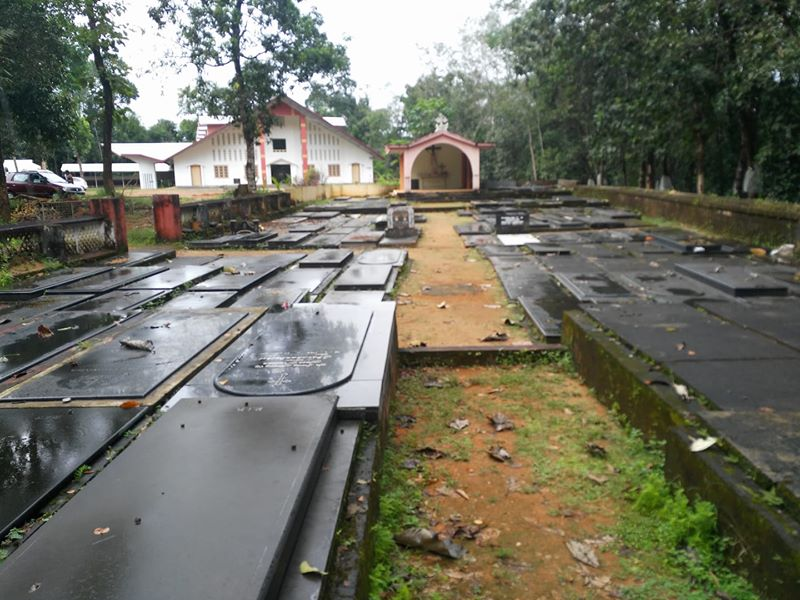
\includegraphics[scale=.25]{images/semitry} 
\label{sem3}
\caption{  }
\end{figure}
   ആദ്യമായി ഇവിടെ വന്ന ഓർമ്മ അമ്മയുടെ അമ്മ മരിച്ചപ്പോഴാണ്. ശവസംസ്കാര ചടങ്ങുകൾ ആദ്യം കാണുന്നതും അന്നാണ്. പിന്നിട് പലപ്പോഴും ഇവിടെ വന്നിട്ടുണ്ട്. ചെറിയ ചുറ്റുമതിലും അവിടവിടെ പൂക്കളുമുള്ള സെമിത്തേരി ചെറുതായിരുന്നപ്പോൾ ഒരു പേടി സ്വപ്നമായിരുന്നു. നാടും നാട്ടുകാരും വികസിച്ചതുസരിച്ച് കാരണവൻമാരുടെ ആസ്ഥാനവും ആളുകൾ പരിഷ്കരിച്ചിട്ടുണ്ട്. പുറംപൂച്ച് കാണിക്കൽ പണ്ടേ നമ്മുടെ ഇഷ്ട വിനോദമാണല്ലോ.
   
    വെളുത്ത മാർബിൾ ഒക്കെ പിടിപ്പിച്ച ഒരാഡ്യൻ കല്ലറയിൽ ഞാൻ കയറിയിരുന്ന് ചുറ്റും നോക്കി. പരിചയക്കാരും കുടുംബക്കാരും ഇടകലർന്ന് താമസിക്കുന്നു. മുപ്പത്തഞ്ചാം വയസിൽ കുത്തേറ്റ് മരിച്ച വല്യപ്പൻ, അമ്പത് കൊല്ലം മുൻപ് ജീപ്പോടിച്ചു പോയപ്പോൾ കൂപ്പ് ലോറി തട്ടി കാഞ്ഞു പോയ പാപ്പൻ, പന്നിംപോത്തും ആവശ്യത്തിന് വെച്ചുതിന്ന് തൊണ്ണുറാം വയസിൽ കാലം ചെയ്ത വെല്യമ്മച്ചി, കാളയുടെ കുത്ത് കൊണ്ട് ചത്ത മത്തൻ ചേട്ടൻ തുടങ്ങി സകല പ്രമാണിമാരേയും കോൺക്രീറ്റ് കുട്ടിനകത്താക്കി മാർബിൾ പതിച്ച് പൂട്ടിയിരിക്കുന്നു. പേരും വീട്ടു പേരും ഒക്കെ ചാപ്പ കത്തീട്ടുണ്ട്. 
    
    അങ്ങനെ നോക്കുമ്പോ സിമിത്തേരിയുടെ അങ്ങേയറ്റത്ത് നിന്ന് ഒരു വല്യപ്പൻ മോണകാട്ടിച്ചിരിക്കുന്നു.
    
    " നി ഏതാടാ കൊച്ചെ ?“ 
    
    "തോണിക്കുഴിലെ “ 
    
    "മാണിച്ചേട്ടനെ ഞാനറിയും. നിനക്കെന്നെ മനസ്സിലായോടാ" 
    
    “ഇല്ല" 
    
    “അതെങ്ങനാ നി കുഞ്ഞാരുന്നപ്പോ ഞാനിവിടെ കയറിയതാ "
    
     " " 
     
     " നിന്റെ കയ്യി ചൊമന്ന വെള്ളം വല്ലോം ഉണ്ടോടാ" 
     
     "ഇല്ല “
     
      “ ഇവിടെ വലിയ പാടാകുവേ എന്തേലും കിട്ടാൻ. കാശൊള്ള ആൾക്കാരെയൊക്കെ കല്ലറക്കകത്താക്കില്ലെ. പുറത്തെറങ്ങാൻ നമ്മളേപ്പോല മൂന്നാല് പാവത്തുങ്ങൾക്കേ പറ്റുന്നുള്ളു. രാത്രിയാകുമ്പോ കപ്യാര് ഗേറ്റ് പുട്ടുകേം ചെയ്യും. നി എവിടുന്നാ വരുന്നേ " 
      
      " തിരുവനന്തപുരത്തുന്നാ “ 
      
      " എന്നാ കൃഷി " 
      
      " കൃഷിയല്ല” 
      
      "പിന്നെ "
      
       "പഠിപ്പിരാ “
      
       "ചക്രം വല്ലോം കിട്ടുവോടാ” 
       
       " ഉം “ 
       
       "ന്നാ അടുത്ത വരവിന് നല്ലതെന്തേലും കൊണ്ടുവരണം ഇവിടെ ആരും ഒന്നും തരുന്നില്ല കാർന്നോമ്മാർക്ക് എല്ലാ ക്കൊല്ലോം ആണ്ട് നടത്താനൊന്നും ആരും ഈ വഴിക്ക് കടക്കുന്നില്ല.” 
       
       പെട്ടെന്ന് ആരോ പിറകിന്ന് പിടിച്ച് എന്നെ വലിച്ചു. ഞെട്ടി തിരിഞ്ഞ് നോക്കിയപ്പം എന്റെ ഒരു കസിനാണ്.
       
        "ഇവിടെയിരിക്കുകയാണോ.ചേട്ടായിനെ ആൾക്കാരന്വോഷിക്കുന്നു. സദ്യ ഒരു റൗണ്ട് കഴിഞ്ഞു. പെട്ടെന്ന് വാ “ 
        
        സിമിത്തേരിന്ന് പുറത്തോട്ടി റങ്ങിയപ്പോൾ ഞാൻ ഒന്നു ടെ തിരിഞ്ഞ് നോക്കി. വല്യപ്പൻ അവിടെത്തന്നെ ഇരുന്ന് ചിരിക്കുന്നു.

\section{ ഭ്രാന്തൻ}
നാട്ടിലുണ്ടായിരുന്ന ഭ്രാന്തൻമാരേക്കറിച്ച് ഓർമിക്കാൻ കാരണം ഇന്ന് നടക്കാൻ പോയപ്പോൾ കീർത്തി നാറാണത്ത് ഭ്രാന്തന്റെ കഥ പറഞ്ഞതാണ്. സ്കൂൾ ലൈബ്രറിയിലെ ഏതോ പുസ്തകം കക്ഷി കഴിഞ്ഞ ആഴ്ച വായിച്ചു. വിശദമായി കഥ പറഞ്ഞു തന്നെങ്കിലും നാറാണത്തു ഭ്രാന്തനെ അവൾ കൃത്യമായി വിഷ്വലൈസ് ചെയ്തോ എന്ന് സംശയമുണ്ട്.
  \begin{figure}[H]
  \center
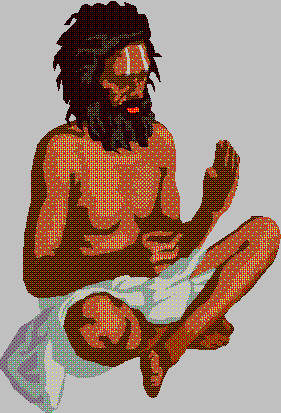
\includegraphics[scale=.3]{images/bhr} 
\label{nv3}
\caption{  ഭ്രാന്തൻ }
\end{figure}
 ചോട്ടാ ബിം ഒക്കെ കാണുന്ന ജനറേഷനല്ലെ. നാറാണത്തിനേപ്പോലെ അലഞ്ഞു തിരിഞ്ഞു നടക്കുന്ന ഒരാളെ അവളിനി കാണുമോയെന്ന് സംശയമാണ്. പറയാൻ വന്നത് എന്റെ ചെറുപ്പകാലത്ത് നാട്ടിലുണ്ടായിരുന്ന രണ്ട് ഭ്രാന്തൻമാരേക്കുറിച്ചാണ്. ഒന്നാമത്തെയാൾകിറുക്കൻ കുഞ്ഞേപ്പ് എന്ന ലക്ഷണമൊത്ത ഭ്രാന്തനായിരുന്നു. താടിയും മുടിയും നീട്ടി വളർത്തി കയ്യിൽ ഒരു ഭാണ്ഡവുമായി അലഞ്ഞു നടക്കും.എന്തൊക്കെയോ പിറുപിറുക്കും. 
 
 വെള്ളിയാമറ്റം സ്കൂളിലേക്ക് പോകുന്ന വഴിയരുകിൽ ഒരു കുപ്പിയുമായി നിന്ന് ഇതിൽ നിറച്ച് കറണ്ടാണ് എന്നുപറഞ്ഞു കൊണ്ടിരുന്ന കുഞ്ഞേപ്പിനെ എനിക്ക് നല്ല ഒർമ്മയുണ്ട്. ഒരു പക്ഷെ എന്റെ സുഹൃത്ത് സജി മാനുവലും ഓർമിക്കുന്നുണ്ടാകും. കുട്ടികളെ പേടിപ്പിക്കാൻ കിറുക്കൻ കുഞ്ഞേപ്പ് പിടിക്കും എന്ന് നാട്ടുകാരൊക്കെ പറയും. ആൾ സാധുവാണ് തനി നാടോടി ആരേയും ഉപദ്രവിച്ച തായി കേട്ടിട്ടില്ല. ഞാൻ ഒൻപതിൽ പഠിക്കുമ്പോൾ കുഞ്ഞേപ്പ് മരിച്ചു. നാറാണത്ത് ഭ്രാന്തൻ സ്റ്റൈലിൽ കൂവക്കണ്ടം ഭാഗത്ത് ഒരു തോട്ടിലാണ് മരിച്ച് കടന്നത്. ഞങ്ങൾ കുട്ടികൾ കാണാൻ പോയെങ്കിലും നാട്ടുകാർ ഓടിച്ചു. 
 
 രണ്ടാമത്തെയാൾ മൈതിനാണ്. കഞ്ചാവടിച്ച് വട്ടായതാണെന്നാണ് കേട്ടിട്ടുള്ളത്. വിറകുവെട്ടാണ് ജോലി. ഇളംദേശം ഭാഗത്തെവിടെയോ ആണ് സ്വദേശം.വലിയ ഒരു മഴുവും ഒരു കെട്ടുമായി വരും. ഷർട്ടൊന്നുമിടില്ല.കഷിക്ക് പൈസയൊന്നു വേണ്ടവയറു നിറച്ച് ഭക്ഷണം കിട്ടിയാൽ മതി. വെട്ടിയിട്ട റബർ മരങ്ങൾ ചെറുതായി മുറിച്ച് അടുക്കി വെക്കുന്ന മൈതീനെ ഇപ്പോഴും ഒർമ്മയുണ്ട്. മൈതിനെ എന്തുകൊണ്ടോ എല്ലാവർക്കും പേടിയായിരുന്നു.അവസാനം എന്തായോ ആവോ.


\section{നക്ഷത്ര വനം}
കഴിഞ്ഞ നൂറ്റാണ്ടിന്റെ അവസാന പകുതിയിൽ കേരള സമൂഹത്തിൽ വേരോടിയ പുരോഗമന ആശയങ്ങളേയും മതനിരപേക്ഷതയേയും അൽപാൽപമായി പിഴുതുമാറ്റാൻ സ്ഥാപിത താൽപര്യക്കാരും സംഘടിത മത ജാതി സംഘടനകളും നിരന്തരമായി ശ്രമിക്കുന്നുണ്ട്. അതിന്റെ ഉദാഹരണങ്ങൾ മെഗാ ഗുരുവന്ദനമായും റോഡിൽ ഇടുന്ന നേർച്ചകളായുമൊക്കെ നാം നിത്യേന കാണുന്നുമുണ്ട്. പല കലാലയങ്ങളിലും അടുത്ത കാലത്തായി തുടങ്ങിയിട്ടുള്ള നക്ഷത്ര വനങ്ങൾ ഇത്തരം ഒരു ശ്രമമായിട്ടാണ് എനിക്ക് തോന്നിയിട്ടുള്ളത്.

പൊതുവേ അന്ധവിശ്വാസങ്ങളോട് ആഭിമുഖ്യമുള്ള ഒരു സമൂഹമാണ് നമ്മുടേത്. നക്ഷത്ര ഫലത്തിനും ജോതിഷത്തിനും നാം ഇപ്പോഴും എന്ത് പ്രാധാന്യമാണ് കൊടുക്കുന്നത്. ജൈവ വൈവിധ്യത്തെ സംരക്ഷിക്കാനെന്ന പേരിൽ ഓരോ മരങ്ങളേയും ഓരോ നക്ഷത്രങ്ങൾക്ക് പതിച്ചു കൊടുക്കുന്നത് എതിർക്കപ്പെടേണ്ടതാണ്. നമ്മുടെ ജൈവ വൈവിധ്യം നൂറ്റാണ്ടുകളായി നക്ഷത്രങ്ങളുടെ സഹായമില്ലാതെ നില നിന്നു പോന്നിട്ടുണ്ട് മനുഷ്യന്റെ ദുരമൂലം സമീപകാലത്ത് ഇതിന് കോട്ടം തട്ടിയിട്ടുണ്ടെങ്കിൽ അത് പരിഹരിക്കുന്നതിന് ബോധപൂർവ്വമായ ശ്രമമാണ് ഉണ്ടാകേണ്ടത്. അല്ലാതെ അന്ധവിശ്വാസങ്ങളെ കെട്ടിയിറക്കുകയല്ല. നമുക്ക് മുമ്പിൽ നാമറിയാതെ ഒരു കാവിക്കണ്ണട വെച്ചു തരാനുള്ള ബോധപൂർവ്വമായ ഒരു ശ്രമമാണ് നക്ഷത്ര വനം.

      \begin{figure}[H]
  \center
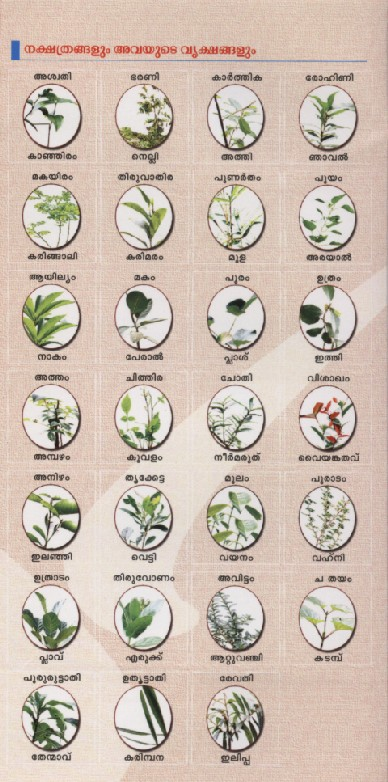
\includegraphics[scale=2]{images/nv} 
\label{nv3}
\caption{  }
\end{figure}
%\section{എൻട്രൻസുപരീക്ഷ }
%
%അടൂത്തവർഷം മക്കളെ എൻട്രൻസുപരീക്ഷ എഴുതിപ്പിക്കാൻ പാടുപെടുന്ന അപ്പൻമാരെ അമ്മമാരെ ഫെയ്സ് ബുക് വിപ്ലവകാരികളെ ഗുണ്ടകളെ, സർക്കാർ നടത്തുന്ന 9 എൻജിനിയറിംഗ്കോളേജുകളിലും സർക്കാർ മേൽവിലാസത്തിൽ നടത്തുന്ന 23 സ്വാശ്രയ കോളേജുകളിലും നിങ്ങൾ മക്കളെ ചേർക്കരുത്. പിള്ളേർ തലച്ചോർ മുരടിച്ച് വല്ല JCB യുടെയൊ ഹെലികോപ്ടറിന്റെയോ ഒക്കെ മുകളിൽ കേറും. SFI യുടെ കൊടി പിടിക്കും. സ്മാൾ അടിച്ച് കുറ്റിക്കാട്ടിൽ ഒക്കെ വാളു വെച്ചു കിടക്കും. നിങ്ങൾക്ക് വേണ്ടി പിള്ളേരേ അടവെച്ച് വിരിയിക്കാൻ പള്ളിലച്ചൻ മാരും കള്ളുമൂതലാളിമാരും നടത്തുന്ന ബ്രോയിലർ ഫാമുകൾ സർക്കാർ ആവശ്യത്തിന് തുടങ്ങിയിട്ടുണ്ടല്ലോ. വരി വരിയായി നിന്ന് പൂക്കളം ഇടാനും സെറ്റുമുണ്ട് ഉടുത്ത് തിരുവാതിര കളിക്കാനും ആൺകുട്ടികൾക്കും പെൺകുട്ടികൾക്കും പ്രത്യേകം സൗകര്യവുമുണ്ട്. പിള്ളേർ സ്മാൾ പോയിട്ട് കോള പോലും അടിക്കത്തില്ല. ഫൈൻ എർപ്പെടുത്തിട്ടുണ്ട് . പിന്നെ പ്രിൻസിപ്പാൾ SSLC ഒക്കെ ബീഹാറീന്ന് ജയിച്ചതാ. ബാക്കി സാറൻമാരൊക്കെ പാവത്തുങ്ങളാ. അച്ചടക്കം അതല്ലെ പ്രധാനം. പിള്ളേരു വാശി പിടിക്കും സർക്കാരിചേരണോന്ന്. വിട്ടു കൊടുക്കരുത് പുണ്യാളന്റെ കോളേജിലൊക്കെ നാലു ലച്ചമാ റേറ്റ്. അഡ്വാൻസ് ബുക്കിംഗ് ഒക്കെ ഉണ്ട്. കരയോഗത്തിനോ പള്ളിന്നോ കത്തുമായി വരീൻ . കണക്കിന്റെ മാർക്കൊക്കെ നമുക്ക് ശര്യാക്കാന്നേ. അച്ചടക്കം ഗ്യാരണ്ടിയാണെ. സീറ്റ് ആണേ പരിമിതോം . എന്നാ ചേരുകല്ലെ?
%
%\section{പോലിസ് അയ്യപ്ൻ }
%കന്യാസ്ത്രികളെ വനിതാ പോലിസിൽ എടുക്കണം. പോലിസ് അയ്യപ്ൻ മാർക്ക് താടി നീട്ടാമെങ്കിൽ ശിരോ വസ്ത്രമിട്ട കന്യാസ്ത്രി പോലിസുമാകാം!എല്ലാവന്റെയും കുരു നിരത്തി പൊട്ടട്ടെ. മതം മണ്ണാങ്കട്ട പൊതു ഇടങ്ങളിൽ നിന്ന് എല്ലാ മത ചിഹ്നങ്ങളും നിരോധിക്കുക . മത വിശ്വാസി വീട്ടിലിരുന്ന് സ്വകാര്യമായി മതം പറയുന്നത് അനുഷ്ടിക്കട്ടെ. പൊതുനിരത്തിലും പൊതു പണം ഉപയോഗിച്ച് നടത്തുന്ന ഇടങ്ങളിലും മതാനുഷ്ഠാനങ്ങളും ചടങ്ങുകളും ഒഴിവാക്കുക.
%
%
%\section{Uniform}
%
%ക്ലാസ് മുറികളിൽ കുട്ടികൾക്ക് യൂണിഫോം ഏർപ്പെടുത്തുന്നതിനോട് വ്യക്തിപരമായി എനിക്ക് യോജിപ്പില്ല. വസ്ത്രം ഒരാളുടെ personal choice ആണ് എന്നു കരുതുന്നു. മെഡിക്കൽപരീക്ഷ നടത്തുമ്പോൾ ക്ലാസ് റൂമുകളിൽ അനുവദിക്കാവുന്ന സ്വകാര്യതക്കും ചോയ്സിനും പരിധി കൽപിക്കുന്നത് തെറ്റല്ല. സമീപകാലത്ത് സംഘടിത മതങ്ങളുടെ അനുയായികൾ സ്വന്തം identity പ്രദർശിപ്പിക്കുന്ന തിന് ഉള്ള മാർഗ്ഗം മായി വസ്ത്രത്തെ മാറ്റിയിട്ടുണ്ട്. ചെറുപ്പക്കാർ എത്ര പെട്ടെന്നാണ് കയ്യിൽ ചരടുകെട്ടുന്നവരും സ്വർണ്ണക്കൊന്ത ഉളുപ്പില്ലാതെ പ്രദർശിപ്പിക്കുന്നവരും ആയി മാറിയത്. വസ്ത്രധാരണ രീതി അടിചേൽപ്പിക്കുന്നതിന് പിന്നിലെ രാഷ്ട്രീയം തിരിച്ചറിയപ്പെടേണ്ടത് തന്നെയാണ്. പൊതു നിയമങ്ങളിൽ നിന്ന് ഒഴിവാകുന്നതിനുള്ള ഒരു excuse ആയി വസ്ത്രത്തെ ദുരുപയോഗം ചെയ്യുന്നത് ഒഴിവാക്കപ്പെടേണ്ടത് തന്നെയാണ്
\section{സ്വപ്നം }

 ഈ നഗരകാന്താരത്തിനാകെ പൊരിച്ച ചിക്കന്റെ മണമാണ്. ആണുങ്ങൾക്ക് പുളിച്ചു റമ്മിന്റെയും പെണ്ണുങ്ങൾക്ക് ഏതോ ഷാമ്പുവിന്റെയും. നാളെ അതിരാവിലെ ഇവിടെ നിന്ന് രക്ഷപെടണം.
 
  പദ്മനാഭനുണരും മുൻപ് ചെക്ക് പോസ്റ്റ് കടക്കണം. അതിർത്തി കടന്നാൽ സ്വാതന്ത്ര്യം. മാർത്താണ്ഡത്തിനപ്പുറം പപ്പനാവന് റേഞ്ചില്ലല്ലോ. തക്കല കഴിഞ്ഞാൽ തോന്നുന്ന വഴികളിലുടെ വണ്ടിയോടിക്കണം . ഇടത്തോട്ടിൻഡിക്കേറ്ററിട്ട് വലത്തോട്ട് തിരിയണം. ആദ്യം കാണുന്ന ചായക്കടയിൽ നിന്ന് ഒരു കാലിയടിക്കണം. ആരും തിരിച്ചറിയാതിരിക്കാൻ വണ്ടി വഴിയിലൊതുക്കി എങ്ങോട്ടെന്നില്ലാതെ അലയണം. അപ്പോൾ ഒരു പച്ചപ്പാടം കാണും. അതിന്റെ നടുവിൽ ഒരു കുന്നും. 
  
  കന്നിൻ മുകളിൽ കിളികളേ നോക്കിയിരിക്കണം. അവരങ്ങനെ പറന്നു പോകാന്നത് ഒരു ചിത്രത്തിലാക്കണം. ചിത്രശലഭങ്ങളോടും തുമ്പികളോടും കിന്നരിക്കണം. കുയിലമ്മക്കൊരെതിർ പാട്ടു പാടണം സൂര്യനുച്ചിയിലെത്തുമ്പോൾ പുഴയിലിറങ്ങി നീന്തണം. ഇതെല്ലാം നാളെ നാളെയെന്ന് വിചാരിച്ചിന്നുറങ്ങുമ്പോൾ സ്വപ്നത്തിലെങ്കിലുമി സ്വപ്നമൊന്ന് സാക്ഷാത്കരിക്കണം.
 
\section{ തേങ്ങ ഉടയ്ക്ക് സ്വാമി}

കാലത്തെ എഴുന്നേറ്റ്  FB പോസ്റ്റിന് ലൈക്ക് കൂടിയോ, ഹർത്തലുണ്ടോ മനസ്സിൽ കിടക്കുന്നതും മരത്തിൽ കണ്ടതുമായ  പോസ്റ്റുകളുടെ ബാക്കി എങ്ങിനെ എഴുതണം എന്നിങ്ങനെ പല വിചാരത്തോടു കൂടി ഫോണിൽ ചുരണ്ടിക്കൊണ്ടിരിക്കുന്നതിനിടയിലാണ് ഒരശരീരി കേട്ടത് " രണ്ട് തേങ്ങ ഉടച്ച് തരണം".

പെട്ടെന്ന് എന്നിലെ കമ്പ്യട്ടർ എൻജിനിയർ ഉണർന്നു. (ബാലമംഗളം വായിച്ച് വായിച്ച് മറവിയുടെ അഗാധ ഗർത്തത്തിലേക്കാണ്ടുപോയ ചില പ്രാചീനചേതനകളും ഇതിന്റെ കൂടെ ഉണർന്നു, പല്ലുതേച്ചു, പത്രം വായിച്ചു.)

ഇന്നത്തേക്ക് വേണ്ട സിരിയസ് FB പോസ്റ്റിന് ഐഡിയ റെഡി. ഈ ന്യൂ ജനറേഷൻ പിള്ളേർക്കൊന്നും മാങ്ങായും തേങ്ങയും തമ്മിൽ തിരിച്ചറിയില്ല. ഇന്ന് തേങ്ങ ഉടയ്ക്കുന്ന അൽഗോരിതത്തേക്കുറിച്ച് ഒരു കുറിപ്പിട്ടേക്കാം.

കേരളത്തിൽ കണ്ടുവരുന്ന സാധാരണ തേങ്ങയ്ക്ക് പരമശിവനുള്ളതുപോലെ മൂന്ന് കണ്ണുകളുണ്ട്. തേങ്ങ ഉടയ്ക്കാനുള്ള ആദ്യപടി ഇതിലെ തൃക്കണ്ണ് കണ്ടു പിടിക്കുക എന്നതാണ്. ഓരോ കണ്ണിലും വെട്ടുകത്തി വെച്ച് പതിയെ കുത്തി നോക്കുക.  
      \begin{figure}[H]
  \center
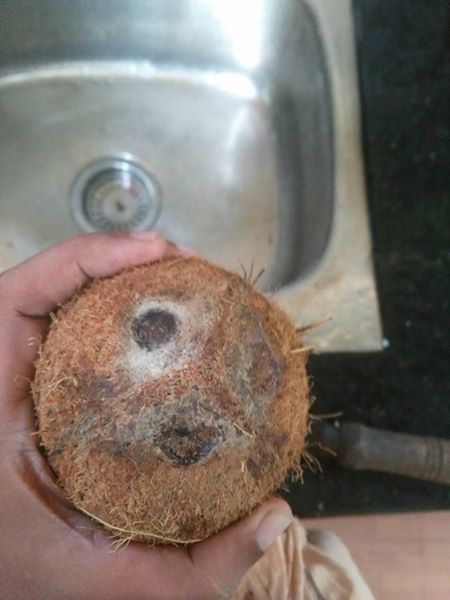
\includegraphics[scale=.25]{images/t1} 
\label{t1}
\caption{  }
\end{figure}
ഇനി തൃക്കണ്ണിനെതിർവശത്തുള്ള വര കണ്ടു പിടിക്കുക. (ചിത്രം ശ്രദ്ധിച്ചോളു.) പെരുവിരൽ തൃക്കണ്ണിൽ വരത്തക്കവിധം തേങ്ങ ഇടതു കയ്യിൽ പിടിക്കുക. എന്നിട്ട് മേൽപറഞ്ഞ വരയുടെ നടുക്ക് വെട്ടുകത്തി കൊണ്ട് ആഞ്ഞടിക്കുക. തേങ്ങ ഉടഞ്ഞിരിക്കും. ഇത് സത്യം സത്യം സത്യം.

      \begin{figure}[H]
  \center
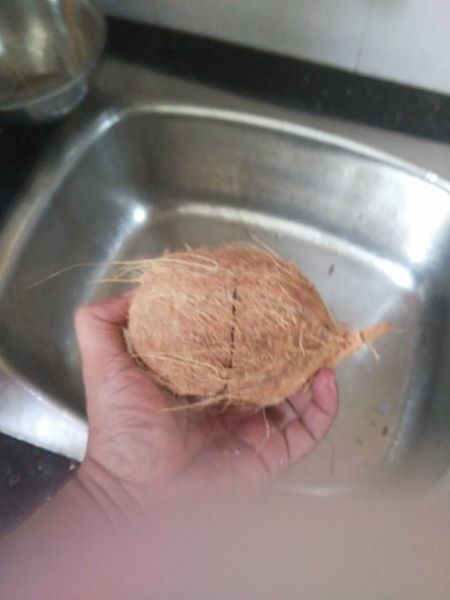
\includegraphics[scale=.25]{images/t2} 
\label{t2}
\caption{  }
\end{figure}

\section{
ആൾദൈവങ്ങളെ ശിക്ഷിക്കാൻ ഭരണകൂടത്തിന് ശക്തിയുണ്ടോ ?}

 ഇല്ല എന്നാണ് എനിക്കു തോന്നിയിട്ടുള്ളത്. യേശുക്രിസ്തുവിനെ വരെ ജനക്കൂട്ടത്തിന് വിടുകയാണ് ഭരണകൂടം ചെയ്തത്. അപ്പോൾ ഭരണം തന്നെ ദൈവങ്ങളുടെ കയ്യിലാണെങ്കിലോ. ദൈവത്തിന് പറ്റിയ ഫൈവ് സ്റ്റാർ ജയിൽ ഇനിയും ഉണ്ടാക്കേണ്ടതുണ്ട്. ഇന്ത്യയിൽമാത്രമല്ല ലോകത്തെമ്പാടും ഇതു തന്നെ അവസ്ഥ. ആൾ ദൈവങ്ങളെ തൊടാൻ ഭരണാധികാരികൾ ഭയപ്പെടുന്നതിന്റെ ഏറ്റവും വലിയ ഉദാഹരണമാണ് ജപ്പാനിലെ ഷോക്കോ അസഹാര എന്ന ദൈവത്തിന്റെ കഥ. 
  \begin{figure}[H]
  \center
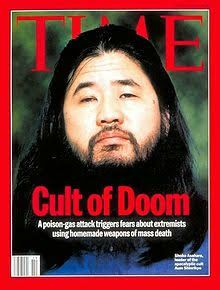
\includegraphics[scale=.45]{images/aal1} 
\label{aal1}
\caption{ ഷോക്കോ അസഹാര }
\end{figure}

   10 വർഷമായി ഇദ്ദേഹത്തെ വധശിക്ഷയ്ക്ക് വിധിച്ചിട്ട്. ഇതുവരെ നടപ്പാക്കാൻ കഴിഞ്ഞിട്ടില്ല. ഇപ്പോൾ ജീവിച്ചിരിക്കുന്ന ആൾദൈവങ്ങളുടെ ഒരു പട്ടികയെടുത്താൽ അതിലെ പുലിയാണ് അസഹാര. ജപ്പാനിലെ ഒരു സാധു കുടുംബത്തിലാണ് കഥാപുരുഷന്റെ ജന്മം. ജന്മനാ ഒരു കണ്ണിന് കാഴ്ചയില്ല. മറ്റേ കണ്ണിന് പകുതി കാഴ്ചയും. അന്ധവിദ്യാലയത്തിലായിരുന്നു വിദ്യാഭ്യാസം. സഹപാഠികൾക്ക് ഇദ്ദേഹത്തെ അന്നേ പേടിയായിരുന്നു. ജപ്പാൻ പ്രധാനമന്ത്രിയാകണമെന്നായിരുന്നു ആഗ്രഹം. പല തവണ കോളജിൽ ചേരാൻ ശ്രമിച്ചു പരാജയപ്പെട്ടു. തുടർന്ന് അക്യപംക്ചർ, ചൈനിസ് വൈദ്യം എന്നിവ പരിശീലിച്ചു. കൂടെ ആൾദൈവങ്ങളുടെ പതിവ് ചെപ്പടി വിദ്യകളും. ഇതിനിടെ കക്ഷി കല്യാണവും കഴിച്ചു പന്ത്രണ്ടു മക്കളുമുണ്ടായി. 
 
   പതിയെ ആൾ ദൈവമായി. ഒരാൾ ദൈവത്തിനു വേണ്ട എല്ലാ ചേരുവകളും ഉപയോഗിച്ചു. പുസ്തകമെഴുത്ത്, ടി വി ചനൽ, യൂണിവേർസിറ്റികളിൽ പ്രസംഗം ഇത്യാദി പരിപാടികൾ തുടരെ നടത്തി. ഇദ്ദേഹത്തിന്റെ ഓം ഷിൻറിക്യോ പ്രസ്ഥാനത്തിലേക്ക്‌ആളുകൾ ഒഴുകിയെത്തി. ഡോക്ടർമാർ, ശാസ്ത്രജ്ഞൻമാർ, രാഷട്രീയക്കാരൊക്കെ ശിഷ്യൻമാരായി. യേശുക്രിസ്തു ആണെന്ന് സ്വയം പ്രഖ്യാപിച്ചു. ലോകത്തിന്റെ മൊത്തം പാപങ്ങൾ ഏറ്റെടുക്കുന്നതിന് വേണ്ടിയാണ് അവതാരം എന്നും പറഞ്ഞു നടന്നു. ബാലമംഗളം പോലെ ഒരു വിശുദ്ധ ഗ്രന്ഥവും എഴുതി. ജൂതന്മാർ. ബ്രിട്ടീഷ് രാജകുടുംബം, ഡച്ചുകാർ മറ്റു മതങ്ങൾ, അമേരിക്കൻ സർക്കാർ ഇവരൊക്കെയായിരുന്നു പ്രധാന ശത്രുക്കൾ.
 
  മൂന്നാം ലോകയുദ്ധം ഉടനുണ്ടാകുമെന്നും അതിനു വേണ്ടി തയ്യാറായിരിക്കണമെന്നും ഉത്ബോധിപ്പിച്ചു. ഇതിനിടെ ചില്ലറ തട്ടിക്കൊണ്ട്, പോകൽ പണം പിടിച്ചുപറിയൊക്കെ മേമ്പൊടിയായി ചേർത്തു. ചിലർക്ക് പരാതി ഉണ്ടായെങ്കിലും ഏതൊരാൾ ദൈവത്തേയും പോലെ രാഷ്ട്രീയ സ്വാധീനവും പോലീസിനുള്ള സ്വാധീനവും കാരണം അന്വേഷണങ്ങൾ എങ്ങുമെത്തിയില്ല. ജപ്പാനിലെ പലരും അദ്ദേഹത്തിന്റെ അനുയായികളായി. ടിവിയിലൊക്കെ live അത്ഭുതങ്ങൾ പ്രദർശിപ്പിച്ചു 1990 കളിൽ ഭരണകൂടത്തെ തന്നെ വെല്ലുവിളിക്കുന്ന ഒരു ശക്തിയായി മാറി. ഒരു പാർട്ടി ഉണ്ടാക്കിയ തിരഞ്ഞെടുപ്പിൽ മത്സരിച്ചു എന്തുകൊണ്ടോ ജപ്പാൻകാർ ഇദ്ദേഹത്തിൽ തോൽപ്പിച്ചു കളഞ്ഞു. ഭരണകൂടവുമായുള്ള ഉരസൽ അപ്പോൾ മുതൽ തുടങ്ങി. അമേരിക്കക്കാർ ഉടൻ ജപ്പാനെ ആക്രമിക്കുമെന്നാണ് അദ്ദേഹം പ്രചരിപ്പിച്ചത്. 
  
  അന്തിമ വിധി (ആർമാഗഡൻ ) ദിവസം ഉടനുണ്ടാകുമെന്നും. 1995 ൽ ടോക്യോ ഭൂഗർഭ റെയിൽവെ ആക്രമിച്ചു കൊണ്ടാണ് അനുയായികൾ അന്തിമ വിധി നടപ്പാക്കാൻ നോക്കിയത്. ഉപയോഗിച്ചത് ചില്ലറ ആയുധമല്ല മാരകമായ രാസായുധം സറിൻ. 13 പേർ നിന്ന നിൽപ്പിൽ മരിച്ചുവീണു. ആയിരക്കണക്കിന് ആളുകൾക്ക് അഗഭംഗമുണ്ടായി. ഇതിനെത്തുടർന്ന് സർക്കാർ അംഹാരയുടെ ആശ്രമവും മറ്റ് പ്രവർത്തനങ്ങളും പരിശോധിച്ചപ്പോൾ കണ്ട കാഴ്ചകൾ  ഞെട്ടിക്കുന്നതായിരുന്നു. രാസായുധങ്ങൾ നിർമിക്കാനുള്ള വൻഫാക്ടറി, പണിയെടുക്കാൻ മികച്ച ശാസ്ത്രജ്ഞർ. ന്യൂക്ലിയർ ആയുധങ്ങൾ തരപ്പെടുത്താനുള്ള വഴിയിലായിരുന്നു അസഹാര. മെട്രോ സബ് വേ ആക്രമണം ജപ്പാനെ തന്നെ പിടിച്ചു കുലുക്കി. അസഹാരയെയും കൂട്ടാളികളെയും പിടികൂടി വിചാരണ ചെയ്തു. വിചാരണ കുറെ നീണ്ടെങ്കിലും 2006ൽ അസഹാരയെ വധശിക്ഷയ്ക്കു വിധിച്ചു. രക്തത്തിൽ ഇരുമ്പിന്റെ അംശം കൂടുതലായതുകൊണ്ടാണെന്നു തോന്നുന്നു ആശാൻ ഇപ്പോഴും ജയിലിൽ തന്നെയുണ്ട്. ഇദ്ദേഹത്തിന്റെ പ്രസ്ഥാനം പേരുമാറ്റി ഇപ്പോഴുമുണ്ട്. 
  
  വധശിക്ഷയൊക്കെ നിയമത്തിന്റെ നൂലാമാലകളിൽ പെട്ടിരിക്കുകയാണ്. നമ്മുടെ ഒരു ചെറുകിട ആൾദൈവത്തിനെ പത്തുവർഷത്തേക്ക് ജയിലിലാക്കിയതിന്റെ പേരിൽ ആഹ്ലാദം പ്രകടിപ്പിക്കുന്നത് കാണുമ്പോൾ എനിക്ക് തോന്നുന്നതിതാണ്. നിങ്ങൾക്ക് ആൾദൈവങ്ങളെ തോൽവിക്കാനാവില്ല മക്കളെ. നിങ്ങൾ വണങ്ങുന്ന ഓരോ പാതിരിയും സ്വാമിയും മൊല്ലയും ഓരോ പൊട്ടൻഷ്യൽ ദൈവങ്ങളാണ്. ജാഗ്രത പാലിച്ചില്ലെങ്കിൽ എപ്പോൾ വേണമെങ്കിലും നിങ്ങളുടെ അന്തിമ വിധി അവർക്കെഴുതാൻ പറ്റും. Pട: ഈ  \href{https://youtu.be/vQ7uz8EYMYo}{ ഡോക്യമെൻററി} ഒന്ന് കണ്ടു നോക്കു. നമ്മുടെ ടി വി ദൈവങ്ങളുമായി സാദൃശ്യം തോന്നിയാൽ ഞാൻ ഉത്തരവാദിയല്ല.  
%

\section{ഒരാൾദൈവം സ്വർഗ്ഗത്തിൽ പോയ കഥ.}  

 ആൾദൈവങ്ങൾ ലോകത്ത് പല സ്ഥലത്തും പല കാലത്തിലും പ്രത്യക്ഷപ്പെട്ടിട്ടുണ്ട്. രാജാവിന്റെ ആത്മീയ ഉപദേശകരായിട്ടോ രാജ്ഞിയുടെ കാമുകനായിട്ടോ ആയിരിക്കും പലപ്പോഴും ഈ അവതാരങ്ങളെ ചരിത്രത്തിൽ രേഖപ്പെടുത്തിയിരിക്കുന്നത്. പണം തട്ടിപ്പ്, ആയുധവ്യാപാരം, അവിഹിതബന്ധം, ബലാൽസംഗം, കുട്ടിക്കൊടുപ്പ്, മാനസിക രോഗം എന്നിവയും അല്പം പ്രത്യശാസ്ത്ര  മത മേമ്പൊടിയും ചേർത്തെടുത്താൽ ആൾ ദൈവം റെഡി. മാർക്കറ്റ് ചെയ്യാൻ നല്ലപോലെ അറിയണം എങ്കിൽ ലോകപ്രശസ്തനാകാം ഹെലികോപ്ടറിൽ പറന്നു നടക്കാം. രാഷ്ട്രീയക്കാരുടെ കൂടെ ഡിന്നറും ലഞ്ചും കഴിക്കാം. വേണമെങ്കിൽ സ്വന്തം രാജ്യം വരെ സ്ഥാപിക്കാം.
 
  എന്തു തെണ്ടിത്തരം കാണിച്ചാലും അനുയായികൾ വാ തുറക്കില്ല, അധികാരികളും. ഇവിടെ മാത്രമല്ല ലോകത്തെമ്പാടും ഇതുതന്നെ സ്ഥിതി. പല മുൻഗാമികളെയും വെച്ചുനോക്കുമ്പോൾ   ഈയിടെ പിടിയിലായ ഹരിയാനക്കാരൻ   റാം റഹീം സിങ് ഒരു ചെറുകിട ആൾദൈവമാണ്. റാം റഹീം സിംഗിനെ കാരണം വെറും 30 പേരല്ലേ സമാധി ആയുള്ളൂ. 
  
  അമേരിക്കൻ ആൾദൈവം ആയിരുന്നു ജിം ജോൺസ് 918 പേരെയും കൊണ്ടാണ് സ്വർഗത്തിലേക്ക് കെട്ടിയെടുത്തത്. അതിൽ മുന്നൂറോളം കുട്ടികളുമുണ്ടായിരുന്നു. നേരിട്ട് സ്വർഗത്തിൽ പോകാൻ ആൾദൈവങ്ങളുടെ അടുത്തേക്ക് ഓടുന്നവർ ജിം ജോൺസിന്റെ കഥ കേട്ടിരിക്കുന്നത് നല്ലതാണ്. ഇരുപതാം നൂറ്റാണ്ടില അമേരിക്കൻ ആൾ ദൈവങ്ങളിൽ പ്രമുഖനായിരുന്നു ജിം ജോൺസ്. മിക്കവാറും എല്ലാ ആൾ ദൈവങ്ങളേയും പോലെ കഷ്ടകാലം പിടിച്ച ബാല്യവും കൗമാരവും ഇദ്ദേഹത്തിനുമുണ്ടായിരുന്നു. സ്വപ്രയത്നം കൊണ്ട് വിദ്യാഭ്യാസം നേടി. പഠനകാലത്തുതന്നെ മറ്റ് കുട്ടികളിൽ നിന്ന് വ്യത്യസ്ഥനായിരുന്നു ജിം . 
\begin{figure}[H]
  \center
\includegraphics[scale=.25]{images/aal2} 
\label{aal2}
\caption{ ജിം ജോൺസ്  }
\end{figure}
  
  ആദ്യ കാലത്ത് കമ്യൂണിസ്റ്റ് ആശയങ്ങളിലും തുടർന്ന് ക്രിസ്തുമത ആശയങ്ങളിലും ആകൃഷ്ടനായി .അറുപതുകളിലും എഴുപതുകളിലും ചെറുകിട തട്ടിപ്പുകളിൽ കൂടി വളർന്നു. നമ്മുടെ ലോക്കൽ ദൈവങ്ങളുടെ അതേ ലൈൻ. ആളേ കൂട്ടാൻ ഫെയ്ത്ത് ഹിലിംഗ്. പാവപ്പെട്ടവരോട് സഹതാപം, സോഷ്യലിസ്റ്റ് നാട്യങ്ങൾ ഒക്കെ ആവശ്യത്തിനുപയോഗിച്ചു. പീപ്പിൾസ് ടെമ്പിൾ എന്നായിരുന്നു ജോൺസിന്റെ കൾട്ടിന്റെ പേര്. രാഷ്ട്രീയക്കാർക്ക് നിരങ്ങാൻ പറ്റിയ സെറ്റപ്പ്. ഇവിടുത്തെ ദൈവങ്ങളെപ്പോലെ തന്നെ ആശാൻ അവാർഡൊക്കെ മേടിച്ചു കൂട്ടി. ഗാന്ധിയുടേയും ബുദ്ധന്റെയും യേശുവിന്റെയും ലെനിന്റെയും ഒരു സങ്കര അവതാരമാണെന്നാണ് സ്വയം വിശേഷിപ്പിച്ചിരുന്നത്. ജോൺസ് അമേരിക്കൻസമൂഹത്തിലെ വംശീയ വിവേചനത്തെ എതിർത്തിരുന്നതുകൊണ്ട് ധാരാളം ആഫ്രോ എഷ്യൻ വംശജർ ശിഷ്യൻമാരായി. കുട്ടികളെ ദത്തെടുക്കുന്നതിന് അനുയായികളെ പ്രേരിപ്പിച്ചു. ജോൺസു തന്നെ കൊറിയൻ വംശജരായ മൂന്ന് കുട്ടികളെ ദത്തെടുത്തു. നമ്മുടെ  റാം റഹീം ബാബായ്ക്ക് പറ്റിയ പോലെ തന്നെ കുറെ കഴിഞ്ഞപ്പോൾ അനുയായികൾ ചിലർ ജോൺസിനോട് തെറ്റി. 
  
  പീപ്പിൾസ് ടെമ്പിളിലെ തിരിമറികളും മനുഷ്യാവകാശ ലംഘനങ്ങളും കുറേശേ പുറം ലോകമറിഞ്ഞു തുടങ്ങി. ഒടുവിൽ ജോൺ സിന് നിൽക്കക്കള്ളിയില്ലാതായി ആയിരത്തിൽ പരം അനുയായികളെയും കുടുംബത്തേയും കൂട്ടി ബ്രിട്ടീഷ് ഗയാനായിലേക്ക് കടന്നു കളഞ്ഞു. ഗയാനയിലെ ഭരണകൂടം ജോൺസിന് സമ്പൂർണ പിന്തുണ കൊടുത്തു. അവിടെ അനുയായികളും ജോൺസും ചേർന്നു ഭൂമിയിലെ സ്വർഗ്ഗം പണിയാൻ ആരംഭിച്ചു. ജോൺസ് ടൗൺ. മുവായിരം ഏക്കറിൽ വമ്പൻ ആശ്രമം. അമേരിക്കയിലേ അനുയായികളോട് ഷോർട്ട് വേവ് റേഡിയോ വഴിയാണ് ജോൺസ് ബന്ധം നിലനിർത്തയത്. ജോൺസ് പാലായനം ചെയ്തെങ്കിലും അമേരിക്കയിലെ പ്രശ്നങ്ങൾ അവസാനിച്ചില്ല.
  
   ജോൺസിന്റെ അനുയായികളിൽ ചിലരുടെ ബന്ധുക്കൾ അലമ്പുണ്ടാക്കി. അനുയായികളിൽ ചിലരെയെല്ലാം ജോൺസ് ഗയാനയിൽ കൊണ്ടുപോയത് പൂർണ്ണ സമ്മതമില്ലാതെയാണ് എന്നൊക്കെ പരാതി വന്നു. കുട്ടത്തിൽ സത്നാംസിങ്ങിന്റെയും നാരായണൻകുട്ടിയുടെയും അമേരിക്കൻ പതിപ്പുകളുമുണ്ടായിരുന്നു. ഈ പരാതികൾ അമേരിക്കൻ കോൺഗ്രസ് അംഗമായ ലിയോ റയാന്റെ ശ്രദ്ധയിൽപ്പെട്ടു. 1978ൽ റയാൻ പിപ്പിൾസ് ടെമ്പിളിലെ മനുഷ്യാവകാശ ലംഘനങ്ങളേക്കുറിച്ച് അന്വോഷിക്കാൻ ഒരു സംഘം മാധ്യമ പ്രവർത്തകരേയും കൂട്ടി ഗയാനയിലേക്ക് പുറപ്പെട്ടു. ഈ സംഘത്തിനെ സ്വീകരിച്ച ജോൺസ് സംഘത്തിനു വേണ്ടി പാർട്ടി നടത്തി. പാർട്ടിക്കിടയിൽ ചില ആളുകൾ അവരെ ജോൺസ് ടൗണിൽ നിന്ന് രക്ഷിക്കണമെന്ന് റയാനോ ടാവശ്യപ്പെട്ടു. ഇതറിഞ്ഞ ജോൺസിന് കലിയിളകി. 
   
   പിറ്റേന്ന് ജോൺസിന്റെ ഒരനുയായി റയാനെ കത്തികൊണ്ട് ആക്രമിച്ചു. ജോൺസ് ടൗണിൽ നിന്ന് രക്ഷപെടുത്തണമെന്ന് ആവശ്യ പ്പെട്ട ചെറിയ ഒരു സംഘത്തോടൊപ്പം റയാൻ തിടുക്കത്തിൽ അടുത്ത എയർപോർട്ടിലേക്ക് പുറപ്പെട്ടു. ജോൺസിന്റെ അനുയായികൾ ഇവരെ പിന്തുടരുന്നുണ്ടായിരുന്നു. എയർപോർട്ടിൽ വച്ച് അതിൽ ഒരാൾ റയാനെ ആക്രമിച്ചു. തുടർന്ന് നടന്ന വെടിവെപ്പിൽ റയാനുൾപ്പെടെ പലരും കൊല്ലപ്പെട്ടു.( ടി വി കാമറമാൻ കൊല്ലപ്പെടുന്നതുവരെ ഇതിന്റെ ചിത്രങ്ങളുണ്ട്. ) കളി കൈ വിട്ടു പോകുകയാണ് എന്ന് തോന്നിയ ജോൺസ് അനുയായികളെല്ലാം വിളിച്ചുകൂട്ടി. നേരിട്ട് എല്ലാവരേയും സ്വർഗത്തിൽ പ്രവേശിപ്പിക്കാൻ തീരുമാനിച്ചു. സോഷ്യലിസവും കമ്യൂണിസവും അതിന്റെ ശുദ്ധമായ രീതിയിൽ നിലനിർത്തുന്നതിന് കൂട്ടമരണമാണ് നല്ലതെന്നോ മറ്റോ ആയിരുന്നു വിശദീകരണം. കുട്ടികൾക്കൊക്കെ സൈനൈഡ് ചേർത്ത് സോഫ്റ്റ് ഡ്രിങ്ക് കൊടുത്തു. മുതിർന്നവർക്ക് സയനയ്ഡ് ഇഞ്ചക്ഷനും. അവസാനം ദൈവം സ്വയം വെടിവെച്ച് മരിച്ചു. 
   
   എഴുപതുകളുടെ അവസാനത്തിൽ ലോകത്തെ പിടിച്ചുകുലുക്കിയ സംഭവമായി രുന്നു ജോൺസ് ടൗൺ കൂട്ടക്കൊല. നമ്മൾ ഹരിയാനക്കാരെയും റാം റഹിംസിംഗിനേയും വെറുതെ പഴിക്കേണ്ട കാര്യമില്ല. രാഷട്രീയ നേട്ടത്തിനായി മതം ഉപയോഗിക്കുന്ന എവിടേയും ഇതൊക്കെ സംഭവിക്കാം. തേക്കും ആടും മാഞ്ചിയവും ചൂടപ്പം പോലെ ചിലവായ ഈ കേരളത്തിലും.
   
    ജോൺസിനെക്കുറിച്ച് നിരവധി പുസ്തകങ്ങളും ഡോക്യമെന്റെറികളും ഇറങ്ങിയിട്ടുണ്ട്. ഈ വിക്കി പേജുകളിൽ വിശദ വിവരങ്ങളുണ്ട്. 
   
   \href{https://en.m.wikipedia.org/wiki/Jim_Jones}{wiki1 }
   
   \href{https://en.m.wikipedia.org/wiki/Jonestown}{wiki2}
     
   \href{https://en.m.wikipedia.org/wiki/Jonestown:_Paradise_Lost}{wiki3}
%
%
%
%കാലനില്ലാത്ത കാലം -------------------------- മനുഷ്യരെല്ലാം ഭീതിയുടെ നോക്കിക്കാണുന്ന അവസ്ഥയാണ് വാർദ്ധക്യം.ജനിച്ചാൽ ഒരു ദിവസം മരിക്കണംഎന്നത് പ്രകൃതി നിയമമാണ് പക്ഷേ ആർക്കും അതിനു മനസ്സില്ല. സമീപകാലത്ത് ശാസ്ത്രത്തിലും സാങ്കേതിക വിദ്യയിലും നേടിയ പുരോഗതി മനുഷ്യന്റെ ശരാശരി ആയുസ്സ് വർധിപ്പിച്ചിട്ടുണ്ട് . സഖാവ് വി എസിനെ പോലെ ചിലരൊക്കെ തൊണ്ണൂറുകളുടെ മധ്യത്തിൽ ചുറുചുറുക്കോടെ നടക്കുന്നുണ്ടെങ്കിലും ഒരു ശരാശരി ഇന്ത്യക്കാരൻ 68 വയസ്സാകുമ്പോഴേക്കും ചിത്രഗുപ്തന്റെ കണക്കു പുസ്തകത്തിലെ ഒരു വരി മാത്രമായിട്ടു ണ്ടാകും.2015ലെ കണക്കനുസരിച്ചാണിത്. അമേരിക്കക്കാരന്റെ ശരാശരി ആയുസ് 78 ഉം ചൈനക്കാരന് 75ഉം ആണ്. മൊണോക്കൊ ക്കാരന് ഇത് 89 ഉം ഛാഡുകാരന് 49 ഉം ആണ് ആ യു സ്. ആർഷഭാരതത്തിൽ മനുഷ്യർക്ക് ആയിരവും പതിനായിരവും വയസുള്ളവരുണ്ടായിരുന്നു എന്നും ഹനുമാൻ ചിരഞ്ചിവിയായിരുന്നു എന്നുമൊക്കെ നമുക്കു് വേണമെങ്കിൽ നമുക്ക് വാദിക്കാം. ഇപ്പോഴത്തെ ട്രെന്റ് അതാണല്ലോ. ( ഞാൻ ഒരിക്കൽ ചരഞ്ചി വിയെ കണ്ടിട്ടുണ്ട്.ഒരു തെലുങ്ക് പടത്തിൽ). ഇനി കാര്യത്തിലേക്ക് കടക്കാം.പ സമീപകാല ശാസ്ത്ര നേട്ടങ്ങളുടെ വെളിച്ചത്തിൽ വാർധക്യം തടയുന്നതിന് വേണ്ടി ധാരാളം റിസർച്ച് നടത്തി തുടങ്ങിയിട്ടുണ്ട് . പല പ്രമുഖരും ഇതിനുവേണ്ടി ഇഷ്ടംപോലെ പണം ഇറക്കിയിട്ടുണ്ട് ( ref 1 ). ഓബ്രി ഡി ഗ്രേ എന്ന ഒരു ബ്രിട്ടിഷ് കമ്പ്യുട്ടർ സയൻറിസ്റ്റ് / ബയോളജിസ്റ്റ് മനുഷ്യായുസ് ആയിരം വർഷം വരെ നീട്ടാം എന്ന് വാദിക്കുന്നവരിൽ പ്രമുഖനാണ്. (ref 3 ). ഒബ്രി 2012 ൽഐഐടി ബോംബെയിൽ വന്നിരുന്നു അന്നാണ് ശാസ്ത്ര സഹായത്തോടെ മനുഷ്യായുസ് നീട്ടുന്ന ഗവേഷണ പദ്ധതികളെപ്പറ്റി ഞാൻ ആദ്യമായി കേൾക്കുന്നത്. ഒബ്രിയുടെ അഭിപ്രായത്തിൽ വാർദ്ധക്യനാശിനി മരുന്നുകളും മെഡിക്കൽ പ്രൊസീഡിയറും മുപ്പത് നാൽപത് വർഷത്തിനുള്ളിൽ കണ്ടു പിടിക്കപ്പെടും. ഒബ്രിയുടെ വിക്കി പേജും പ്രസംഗത്തിന്റെ വിഡിയോ ലിങ്കും താഴെ കൊടുത്തിട്ടുണ്ട്. (Ref 4,5 ) അന്നു മുതൽ ഈ വിഷയത്തിൽ വരുന്ന ഗവേഷണപ്രബന്ധങ്ങളും വാർത്തകളും ശ്രദ്ധിക്കാറുണ്ട് . ആയിരമൊന്നും കിട്ടിയില്ലേലും ഒരു നൂറു കൂടി തടഞ്ഞാൽ കൊള്ളാം. നൂറു കൊല്ലം കഴിഞ്ഞ് എല്ലാ വരേയുംകണ്ടു മുട്ടാമെന്ന് പ്രതീക്ഷയുണ്ട്. അപ്പോൾ കുഞ്ചൻ നമ്പ്യാർ പറഞ്ഞതുപോലെ മുത്തച്ഛൻ മുതുക്കന്റെ മുത്തച്ഛൻ മരിച്ചില്ലഅവനുണ്ട് മുത്തച്ഛൻ മരിച്ചില്ല എന്ന് പടേണ്ടി വരും. Pട: ഹനുമാന്റെ ജീവിതചര്യകളും ചിരഞ്ചി വി യുടെ തെലുങ്കു പടങ്ങളും ആർഷഭാരത സംസ്കാരത്തിൽ ചെലുത്തിയ സ്വാധീനം എന്ന വിഷയത്തിൽ ഗവേഷണം നടത്താൻ കേന്ദ്ര ഗവർമെന്റ് ഫണ്ട് ചെയ്യാൻ സാധ്യതയുണ്ട്. താൽപര്യമുള്ളവർക്ക് അപേക്ഷിക്കാം. Ref: 1)http://www.lifeextension.com/magazine/2015/10/billionaire-philanthropists-funding-anti-aging-research/page-01 2) https://www.sciencedaily.com/releases/2017/03/170323141340.htm 3) https://en.m.wikipedia.org/wiki/Aubrey_de_Grey 4) http://www.sens.org 5) https://youtu.be/PJqcIFkBsxs

\chapter{പകുതി വഴി നിന്നുപോയവ }

\section{ ചന്ദ്രനും ജനാർദ്ദനനും }

\section{ ചെന്നായ്കളും പുലിയും } 

\section{പങ്കുകള്ള് }

\section{സാഹിബ് ബീബി ഓർ ഗുലാം} 

\section{ മുണ്ടു പുരാണം }

\section{ബൾബും പോലീസും }

\section{അരിയിട്ട് പിടിച്ച കോഴി }
\section{നുണപറയുന്നവർ }
\section{Stories of Padamarajan}
\section{സ്ഥലത്തെ പ്രധാന ദിവ്യൻ }


\end{document}

